\documentclass[type=doctor]{thuthesis}
% 选项:
%   type=[bachelor|master|doctor|postdoctor], % 必选
%   secret,                                   % 可选
%   pifootnote,                               % 可选(建议打开)
%   openany|openright,                        % 可选,基本不用
%   arial,                                    % 可选,基本不用
%   arialtoc,                                 % 可选,基本不用
%   arialtitle                                % 可选,基本不用

% 所有其它可能用到的包都统一放到这里了,可以根据自己的实际添加或者删除。
\usepackage{thuthesis}
\usepackage{array}
\newcommand{\PreserveBackslash}[1]{\let\temp=\\#1\let\\=\temp}
\newcolumntype{C}[1]{>{\PreserveBackslash\centering}p{#1}}
\newcolumntype{R}[1]{>{\PreserveBackslash\raggedleft}p{#1}}
\newcolumntype{L}[1]{>{\PreserveBackslash\raggedright}p{#1}}

% 定义所有的图片文件在 figures 子目录下
\graphicspath{{figures/}}

% 可以在这里修改配置文件中的定义。导言区可以使用中文。
% \def\myname{薛瑞尼}

\begin{document}

%%% 封面部分
\frontmatter
\thusetup{
  %******************************
  % 注意:
  %   1. 配置里面不要出现空行
  %   2. 不需要的配置信息可以删除
  %******************************
  %
  %=====
  % 秘级
  %=====
  secretlevel={秘密},
  secretyear={10},
  %
  %=========
  % 中文信息
  %=========
  ctitle={卷积神经网络:组合卷积结构、随机区域池化和模型压缩},
  cdegree={工学博士},
  cdepartment={计算机科学与技术系},
  cmajor={计算机科学与技术},
  cauthor={王振扬},
  csupervisor={邓志东教授},
  %cassosupervisor={陈文光教授}, % 副指导老师
  %ccosupervisor={某某某教授}, % 联合指导老师
  % 日期自动使用当前时间,若需指定按如下方式修改:
  % cdate={超新星纪元},
  %
  % 博士后专有部分
  %cfirstdiscipline={计算机科学与技术},
  %cseconddiscipline={系统结构},
  %postdoctordate={2009年7月——2011年7月},
  %id={编号}, % 可以留空: id={},
  %udc={UDC}, % 可以留空
  %catalognumber={分类号}, % 可以留空
  %
  %=========
  % 英文信息
  %=========
  etitle={Convolutional Neural Network:  Module Combination Convolution, Stochastic Area Pooling, and Model Compression},
  % 这块比较复杂,需要分情况讨论:
  % 1. 学术型硕士
  %    edegree:必须为Master of Arts或Master of Science(注意大小写)
  %             “哲学、文学、历史学、法学、教育学、艺术学门类,公共管理学科
  %              填写Master of Arts,其它填写Master of Science”
  %    emajor:“获得一级学科授权的学科填写一级学科名称,其它填写二级学科名称”
  % 2. 专业型硕士
  %    edegree:“填写专业学位英文名称全称”
  %    emajor:“工程硕士填写工程领域,其它专业学位不填写此项”
  % 3. 学术型博士
  %    edegree:Doctor of Philosophy(注意大小写)
  %    emajor:“获得一级学科授权的学科填写一级学科名称,其它填写二级学科名称”
  % 4. 专业型博士
  %    edegree:“填写专业学位英文名称全称”
  %    emajor:不填写此项
  edegree={Doctor of Philosophy},
  emajor={Computer Science and Technology},
  eauthor={Wang Zhenyang},
  esupervisor={Professor Deng Zhidong},
  %eassosupervisor={Chen Wenguang},
  % 日期自动生成,若需指定按如下方式修改:
  % edate={December, 2005}
  %
  % 关键词用“英文逗号”分割
  ckeywords={计算机视觉, 深度学习, 卷积神经网络},
  ekeywords={Computer Vision, Deep Learning, Convolutional Neural Networks}
}

% 定义中英文摘要和关键字
\begin{cabstract}
  
 近年来,卷积神经网络在计算机视觉、自然语言处理、语音识别等诸多领域均取得了突破性研究进展。特别是在视觉物体识别任务上,随着标注数据的积累和GPU计算性能的提升,使得卷积神经网络研究取得了多个
 特别是在视觉物体识别任务上,卷积
  卷积神经网络在计算机视觉领域,尤其是视觉物体识别任务上,取得了突破性研究进展。本文针对视觉物体识别问题,研究了卷积神经网络在结构和方法上的改进。 取得的主要研究成果包括:
  
  \begin{itemize}
    \item 提出了组合卷积结构来简化深层网络结构的设计过程,弱化网络设计过程中的感受野和深度选择问题。组合卷积结构是一种多个模型的组合结构,集成了盗梦空间结构Inception、最大化输出单元Maxout、残差网络模型ResNet和网络中的网络NIN 四个著名卷积模型的优势。组合卷积结构由四条不同的特征提取分支和一个特征选择器构成。其中包括两条具有不同深度和感受野大小的卷积分支,一条残差分支用于加快网络的收敛速度,一条Maxout分支用于增强模型的非线性拟合能力,最后通过一个选择器对特征进行筛选与组合。
    \item 提出了一个由随机区域池化和T型网络结构组成的网络模型。在随机区域池化方法中,采用由仿射变换随机生成的池化区域来代替原来固定不变的池化区域,但是仍然保留了传统的池化操作即最大池化或均值池化。随机区域池化可以看做是对中间层特征的一种重采样方法,起到特征増广的目的。同时我们提出一种通用的网络结构T型结构,可以有效地避免网络设计过程中的特征表达瓶颈问题。
    \item 提出了一种基于主导卷积核分解和知识预回归的模型压缩方法来加快网络的预测时间。主导卷积核分解是一种受矩阵低秩分解启发的卷积参数压缩方法。知识预回归通过将知识从教师网络迁移到压缩后学生网络,让学生网络逐层地学习教师网络的泛化能力,尽量弥补学生网络因参数压缩所造成的精度损失。
   \end{itemize}

 最后,我们以交通标志识别为应用背景,对组合卷积结构和随机区域池化进行了测试与验证。并且将两种方法结合,应用于德国交通标志识别数据集GTSTB上,取得了99.66\%的测试精度。进一步采用主导卷积核分解与知识预回归的方法对模型进行压缩与加速,最终取得了近10倍的模型压缩率和预测速度提升,并且保持了一个较高的识别精度99.27\%。
 
 \end{cabstract}

% 如果习惯关键字跟在摘要文字后面,可以用直接命令来设置,如下:
% \ckeywords{\TeX, \LaTeX, CJK, 模板, 论文}

\begin{eabstract}

Convolutional neural networks play an increasingly important role in computer vision tasks, especially in the field of visual object recognition. In this dissertation, we study on the improvements of convolutional neural networks for visual object recognition. The innovative achievements for this dissertation include:

  \begin{itemize}
    \item We propose a novel module called self-adaptive module (SAM) to simplify design of any new deep learning architecture, since it no longer requires consideration of how to select receptive fields and depths. SAM is a combination of five prominent models, such as Inception, Maxout, ResNet, and NIN. It consists of four passes and one selector. Specifically, the four passes include two direct passes with different receptive fields and depths, one residual pass, and one Maxout pass. Actually, the residual pass is used to speed up convergence, while we take advantage of the Maxout pass to enhance approximate capabilities of SAM. The selector is further designed to help choose reasonable output.
    \item We propose a novel network model that incorporates a stochastic area pooling (SAP) method with a generic stacked T-shaped CNN architecture. In our SAP method, pooling area is randomly transformed and max pooling operation is then conducted on such areas, which means that regular pooling area of fixed upright squares are no longer exploited in the training phase of our SAPNet. In a sense, it could be viewed as the use of feature-level augmentation. Meanwhile, we present a generic CNN architecture that structurally resembles three stacked T-shaped cubes. In such architecture, the number of kernels in convolutional layer preceding any pooling layer is doubled to prevent the representational bottleneck problem.
    \item Aiming at accelerating the test time of deep convolutional neural networks, we propose a model compression method that contains a novel dominant kernel (DK) and a new training method called knowledge pre-regression (KP). DK is presented to significantly accomplish a low-rank decomposition of convolutional kernels, while KP is employed to transfer knowledge of intermediate hidden layers from a larger teacher network to its compressed student network on the basis of a cross entropy loss function instead of previous Euclidean distance.
  \end{itemize}

Finally, we demonstrate the effectiveness of our methods for traffic sign classification. On GTSRB dataset, we achieve a test accuracy of 99.66\%, and compress the number of parameters by a factor about 10. The compressed network is 10 times faster than before, and achieve a test accuracy of 99.27\%.


\end{eabstract}

% \ekeywords{\TeX, \LaTeX, CJK, template, thesis}

% 如果使用授权说明扫描页,将可选参数中指定为扫描得到的 PDF 文件名,例如:
% \makecover[scan-auth.pdf]
\makecover

%% 目录
\tableofcontents

%% 符号对照表
\begin{denotation}[3cm]
\item[AI] 人工智能 (Artificial Intelligence)
\item[ML] 机器学习 (Machine Learning)
\item[NN] 人工神经网络 (Neural Networks)
\item[DL] 深度学习 (Deep Learning)
\item[DNN] 深度神经网络 (Deep Neural Network)
\item[CNN] 卷积神经网络 (Convolutional Neural Network)
\item[CV] 计算机视觉 (Computer Vision)
\item[SAM] 自适应卷积模块 (Self-Adaptive Convolutional Module)
\item[SAP] 随机区域池化 (Stochastic Area Pooling)
\item[DK] 主导卷积核 (Dominant Convolutional Kernel)
\item[KP] 知识预回归 (Knowledge Pre-Regression)
\item[ILSVRC] ImageNet大规模视觉识别比赛 (ImageNet Large Scale Visual Recognition Competition)
\item[SVHN] 街景房牌号 (The Street View House Numbers)
\item[GTSRB] 德国交通标志数据集 (German Traffic Sign Recognition Benchmark)
\item[GMDH] 分组数据处理 (Group Method of Data Handling)
\item[NIN] 网络中的网络 (Network in Network)
\item[RF] 感受野 (Receptive Field)
\item[MLP] 多层感知机 (Multi-Layer Perceptron)
\item[ReLU] 线性整流单元 (Rectifier Linear Unit)
\item[LReLU] 斜坡线性整流单元 (Leaky Rectifier Linear Unit)
\item[PReLU] 参数化线性整流单元 (Parametric Rectifier Linear Unit)
\item[RReLU] 随机线性整流单元 (Randomized Rectifier Linear Unit)
\item[ELU] 指数线性整流单元 (Exponential Linear Unit)
\item[LRN] 局部响应正则化 (Local Response Unit)
\item[BN] 批正则化 (Batch Normalization)
\item[GPU] 图形处理器 (Graphic Processing Unit)
\item[BP] 反向传播算法 (Back-Propagation)
\item[SIFT] 尺度不变特征变换 (Scale Invariant Feature Transform)
\item[HOG] 方向梯度直方图 (Histogram Based Saliency)
\item[SGD] 随机梯度下载 (Stochastic Gradient Descent)
\item[SVM] 支持向量机 (Support Vector Machine)
\item[UGV] 无人地面车 (Unmanned Ground Vehicle)
\item[ADAS] 高级辅助驾驶 (Advanced Driver Assistance Systems)
\end{denotation}



%%% 正文部分
\mainmatter
\chapter{绪论}
\label{cha:introduction}

\section{研究背景与意义}
\label{sec:intro}

1956,在达特茅斯会议会议上,约翰·麦卡锡等人提出了人工智能(Artificial Intelligence,AI)的概念,开辟了如今人工智能这一领域学科。当时,科学家们希望打造一台可以像人一样思考的机器,即所谓的通用人工智能。现如今,虽然我们还没有实现这个伟大的目标,但是六十年的研究与探索,在一些特定的任务上,机器已经可以取代甚至超越人类。2011年,沃森在美国智力问答节目《危险边缘》中轻松战胜了两位人类冠军,展现出人工智能在自然语言理解方面的重大突破。2016年,谷歌旗下深度思维公司研发的Alfago机器人,在围棋人机对战中,以4比1的成绩击败了世界排名第五的李世石,成为人工智能研究工作的另一个里程碑。

机器学习(Machine Learning,ML)是实现人工智能的一种有效方式。机器学习是一个涉及多个领域的交叉学科,目前并没有统一的定义。一种常见的解释是,机器学习通过模拟、归纳人类的学习行为,利用计算机强大的计算能力,让机器从大规模的数据中获取知识,不断提升机器自己的性能最终获得执行任务的能力。机器学习多年的发展历程中,演化出诸多经典算法,例如决策树、贝叶斯分类、支持向量机、最大期望算法等。早期的这些算法均没有实现人工智能的终极目标,甚至在狭义人工智能的一些特定的任务上,也很难达到人类水平。深度学习(Deep Learning,DL)的出现,改变了这一现状。

深度神经网络(Deep Neural Network,DNN)起源于人工神经网络(Neural Networks,NN),是受生物神经科学启发演化出的计算模型。人工神经网络借鉴了神经系统中神经元和突出连接等微观概念,从而提出了“感知器”(Perceptron)计算模型,但是当时人工神经网络对脑科学的认知并不够深刻。深度神经网络试图通过模拟信息在大脑神经元之间的传播过程,借鉴人脑分层化的信息处理机制,提出了由多层“感知器”组成的计算模型即多层感知器。深度神经网络采用分层的特征提取方式,在人工智能应用领域取得了最大的成功。

计算机视觉(Computer Vision,CV)是人工智能领域研究热点之一,也是深度神经网络取得巨大成功的应用领域之一。计算机视觉是一门研究如何让计算机模拟生物视觉来理解世界的科学,采用各种成像设备代替人的视觉感官,获取周围的环境信息为做系统的输入,例如通过相机获取的RGB图像、通红外线获取的红外图像、通过热红外获取的热图等,再通过计算机强大的计算能力来模拟人脑对环境的处理和理解,让计算机可以具有某种程度上的智能去完成一些特定的任务。受生物视觉系统启发,将局部感受野、权值共享、池化和分层特征提取等概念融入其中的卷积神经网络(Convolutional Neural Network,CNN)极大地促进了计算机视觉的发展与进步。卷积神经网络是深度神经网络的一个研究分支,也是目前计算机视觉领域的研究热点之一。此外,卷积神经网络在语音识别、视觉物体识别、物体检测和基因组识别等领域中也取得巨大的成功,在人脸识别、自然语言处理和围棋人机对战中,甚至取得了超越人类的水平,让我们对狭义人工智能的发展与到来,充满了信心与期待。

\section{相关研究}
\label{sec:relate}


1943年,McCulloch等人~\cite{mcculloch1943logical}最先提出了神经网络的理论模型,当时的神经网络还不具备学习的能力。1958年,康奈尔大学的Rosenblatt~\cite{rosenblatt1958perceptron}教授提出了“感知器”(Perceptron)计算模型,被认为是神经网络的始祖。据我们所知,第一个深层的神经网络是Ivakhnenko等人~\cite{ivakhnenko1966cybernetic,ivakhnenko1967cybernetics,ivakhnenko1968group,ivakhnenko1971polynomial}提出的,1971年,在其发表的重要学术论文\cite{ivakhnenko1971polynomial}中,就已经提出了一个具有八层之深的分组数据处理(Group Method of Data Handling,GMDH)多层感知器。%1975年,日本学者Fukushima提出认知机(Cognitron)~\cite{fukushima1975cognitron} 和神经认知机(Neocognitron)~\cite{fukushima1980neocognitron}模型,被认为是最早的卷积神经网络原型。

1969年,在Minsky和Papert~\cite{minsky1969perceptrons}发布的新书《感知器》中,论证了感知器存在的两个关键问题:单层的感知器无法解决复杂的非线性问题,其中提到了经典的异或操作;另外当时的计算能力也无法满足感知机的计算需求。神经网络的研究一度陷入低潮,发展缓慢,直到误差反向传播(Backpropagation,BP)算法的出现,改变了这种现象。最早的BP算法是Linnainmaa~\cite{linnainmaa1970representation,linnainmaa1976taylor}在其1970年的博士论文中提出的,当时的BP并没有用在神经网络。1973年,Dreyfus~\cite{dreyfus1973computational}将BP算法应用于最小化误差函数。据我们所知,第一个将BP应用于神经网络的算法是Werbos~\cite{werbos1982applications}于1982年提出的。但是1985年,Rumelhart和Hinton等人的论文~\cite{rumelhart1985learning}才使得神经网络的BP算法得到了广泛的关注,为神经网络的发展做出了重大的贡献。


%近年来对神经网络的研究,主要可以分为三个流派,分别是:基于概率模型的神经网络模型,基于数据或特征重构的自动编码器,和目前最受关注的卷积神经网络。

%\subsection{基于概率模型的神经网络模型}
%从概率模型观点出发,特征学习的过程可以理解为,通过对大量输入数据的观察,找到一组可以正确表示输入数据样本分布的隐层特征。对于隐层特征$h$和观测数据$x$,对$h$和$x$的联合概率分布$p(x,h)$进行建模。特征提取的过程可以看成在已知输入数据$x$的情况下,预测隐层随机变量$h$概率分布的过程,即求解后验概率分布$p(h|x)$。学习的过程可以看做是采用极大似然估计的方法,对模型参数求解的过程。概率图模型采用图结构来描述随机变量之间的依赖关系,可以分为有向概率图和无向概率图两类。它们的区别仅仅体现在联合概率的定义,但两者学习的过程和计算量却截然不同。

%有向概率图模型可以统一解释为,在已知条件概率分布$p(x|h)$和先验概率分布$p(h)$的情况下,重构联合概率$p(x,h)=p(x|h)p(h)$的过程。基于有向概率图模型的网络包括:概率主成分分析(Probabilistic Principal Component Analysis ,PPCA)~\cite{tipping1999probabilistic}、概率解释的稀疏编码~\cite{olshausen1996emergence}、Sigmoid信念网络(Sigmoid Belief Networks)~\cite{neal1992connectionist}和深度信念网络(Deep Belief Network、DBN)~\cite{hinton2006reducing}。其中概率主成分分析和概率解释的稀疏编码常常被当做深度学习发展过程中的浅层学习网络。在概率主成分分析中,假设预测数据$x$是由隐层随机变量$h$生成的,并且隐层变量$h$和条件概率$p(x|h)$均服从高斯分布:
%\begin{eqnarray} \label{equ:ppca}
%p(h)&=&\mathit{N}(h|0,\sigma_{h}^{2}\mathit{I})\nonumber\\
%p(x|h)&=&\mathit{N}(x|Wh+\mu_x,\sigma_{x}^{2}\mathit{I})
%\end{eqnarray}
%概率解释的稀疏编码与此类似,但是隐层随机变量$h$不再服从高斯分布,而是服从稀疏诱导的拉普拉斯先验(Sparsity Inducing Laplace prior):
%\begin{eqnarray} \label{equ:psc}
%p(h)&=&\prod_{i}^{d_h}exp(-{\lambda}{\lvert}h_i{\rvert})\nonumber\\
%p(x|h)&=&\mathit{N}(x|Wh+\mu_x,\sigma_{x}^{2}\mathit{I})
%\end{eqnarray}
%借鉴于视觉皮层对复杂刺激的响应方式,Olshausen指出,经稀疏编码提取的图像基函数类似于生物视觉皮层V1区简单细胞的响应特性:局限性、方向性和选择性。

%无向概率图模型,即马尔科夫随机场(Markov Random Fields,MRFs),其联合概率$p(x,h)$可以表示为:
%\begin{eqnarray} \label{equ:mrf}
%p(x,h)=\frac{1}{Z_\theta}{\prod_i\psi_i(x)}{\prod_j\eta_j(h)}{\prod_k\upsilon_k(x,h)}
%\end{eqnarray}
%其中$\psi_i(x)$,$\eta_j(h)$和$\upsilon_k(x,h)$分别表示观测数据$x$,隐随机变量$h$和它们之间相互作用的群势能(Clique Potentials);$Z_\theta$为归一化因子。玻尔兹曼机(Boltzmann)~\cite{hinton1983optimal}是MRFs的一种简化形式,可以表示:
%\begin{eqnarray} \label{equ:bz}
%p(x,h)=\frac{1}{Z_\theta}exp(-\varepsilon_\theta(x,h))
%\end{eqnarray}
%其中$\varepsilon_\theta(x,h)$是能量函数;$\theta$是模型的参数。波尔兹曼机的能量通常定义为:
%\begin{eqnarray} \label{equ:bm_e}
%\varepsilon_\theta(x,h)^{BM}=-\frac{1}{2}x^{T}Ux-\frac{1}{2}h^{T}Vh-x^{T}Wh-b^{T}x-d^{T}h
%\end{eqnarray}
%其中参数$\theta=(U,V,W,b,d)$是模型的参数,分别代表观测层对观测层、隐层对隐层、观测层对隐层、观测层自身和隐层自身的连接关系。受限波尔兹曼机(Restricted Boltzmann Machine,RBM)是对波尔兹曼机的一种简化,也是最常见得波尔兹曼机计算模型。RBM的能量函数$\varepsilon_\theta(x,h)^{RBM}$仅仅是令$\varepsilon_\theta(x,h)^{BM}$中的$U=0, V=0$。与RBM相关的研究主要集中于模型的改进与学习算法两个方向。在模型方面,包括高斯受限玻尔兹曼机(GRBM)~\cite{krizhevsky2009learning}、均值方差受限玻尔兹曼机(mcRBM)~\cite{hinton2010modeling}、mPoT模型~\cite{mnih2010generating}、钉板(Spike-and-Slab)受限玻尔兹曼机(ssRBM)~\cite{courville2011spike}和深度玻尔兹曼机(Deep Boltzmann Machine、DBM)。在学习方法上包括吉布斯采样法(Gibbs Sampling)~\cite{hinton1983optimal}、对比离差算法(Contrastive Divergence,CD)~\cite{hinton1999products,hinton2006fast}、随机最大似然法(Stochastic Maximum Likelihood、SML)~\cite{younes1999convergence}、快速持续对比离差算法(Fast-weights Persistent Contrastive Divergence,FPCD)~\cite{tieleman2009using}。
%
%
%概率模型的学习需要求隐随机变量相对于观测变量的后验概率,不论在有向图模型还是无向图模型,后验概率的计算是很复杂甚至于无法计算的,尤其是对于深层网络结构。因此通常采用采样的方法对其进行估计,这往往会引入估计误差。自动编码器(Autoencoders)~\cite{bourlard1988auto,hinton1994autoencoders}是一种直接对数据数据进行重构的特征提取方法,包括编码(encoder)和解码(decoder)两个过程,将编码和解码函数分别记为$f_\theta$和$g_\theta$,其中$\theta$是需要学习的参数。一个最基本的自动编码器可以通过最小化重构误差函数求解:
%\begin{eqnarray} \label{equ:ae}
%\mathcal{J}_{AE}(\theta)=\sum_{t}L(x^{(t)},g_{\theta}(f_{\theta}(x^{(t)})))
%\end{eqnarray}
%其中$x^{(t)}$是训练样本;$L$为L1或L2范数。与自动编码器相关的研究主要包括稀疏自动编码器(Sparse Autoencoders,SAE)~\cite{poultney2006efficient}、去噪自动编码器(Denoising Autoencoders,DAE)~\cite{vincent2008extracting}收缩自动编码器(Contractive Autoencoders,CAE)~\cite{rifai2011contractive}预测自动编码器(Predictive Sparse Decomposition,PSD)~\cite{olshausen1996emergence}等,这些方法的主要区别在于优化函数有所不同:
%\begin{eqnarray} \label{equ:aes}
%\mathcal{J}_{SAE}(\theta)&=&\sum_{t}L(x^{(t)},g_{\theta}(f_{\theta}(x^{(t)})))+\lambda\sum_{t}\lVert{h^{(t)}}\lVert_{1}\nonumber\\
%\mathcal{J}_{DAE}(\theta)&=&\sum_{t}\mathbb{E}_{q(\tilde{x}|x^{(t)})}[L(x^{(t)},g_{\theta}(f_{\theta}(x^{(t)})))]\nonumber\\
%%\mathcal{J}_{CAE}(\theta)&=&\sum_{t}L(x^{(t)},g_{\theta}(f_{\theta}(x^{(t)})))+\lambda\vert\vert{f_{\theta}(x)_j(1-f_{\theta}(x)_j)W_j}\vert\vert_{F}^{2}
%\mathcal{J}_{CAE}(\theta)&=&\sum_{t}L(x^{(t)},g_{\theta}(f_{\theta}(x^{(t)})))+\lambda\lVert{\frac{\partial{f_\theta}}{\partial{x}}(x)}\rVert_{F}^{2}\nonumber\\
%\mathcal{J}_{PSD}&=&\sum_{t}\lVert{h^{(t)}}\lVert_{1}+\lVert{x^{(t)}-Wh^{(t)}}\lVert_{2}^{2}+\lVert{h^{(t)}-f_{\alpha}(x^{(t)})}\lVert_{2}^{2}
%\end{eqnarray}

%\subsection{卷积神经网络研究进展}

卷积神经网络是受生物视觉皮层认知机制启发而来,1959年,Hubel和Wiesel~\cite{hubel1959receptive,hubel1962receptive}在生物视觉皮层的早期研究中,发现了在感受野范围内视觉皮层中简单细胞、复杂细胞和超复杂细胞对光信号具有不同的响应。受此启发,日本学者Fukushima于1975年提出了认知机(Cognitron)~\cite{fukushima1975cognitron} 和神经认知机(Neocognitron)~\cite{fukushima1980neocognitron}的计算模型,通常被认识是最早的卷积神经网络原型。1989年,LeCun等人~\cite{lecun1989backpropagation,le1990handwritten}将误差反向传播算法引入到神经认知机模型中,提出了著名的LeNet-5网络,如图~\ref{fig:lenet}所示,奠定了现代卷积神经网络的计算框架。但由于当时训练数据规模和计算机计算能力的限制,卷积神经网络并没有受到广泛的关注。2012年,Krizhevsky等人~\cite{krizhevsky2012imagenet}提出了一个与LeNet-5类似,但结构更深的卷积神经网络模型艾利克斯网络AlexNet,借助于高性能的GPU并行计算能力,在2012年ImageNet大规模视觉识别比赛(ImageNet Large Scale Visual Recognition Competition,ILSVRC)中一举夺冠,掀起了卷积神经网络的研究热潮。

\begin{figure*}
\centering
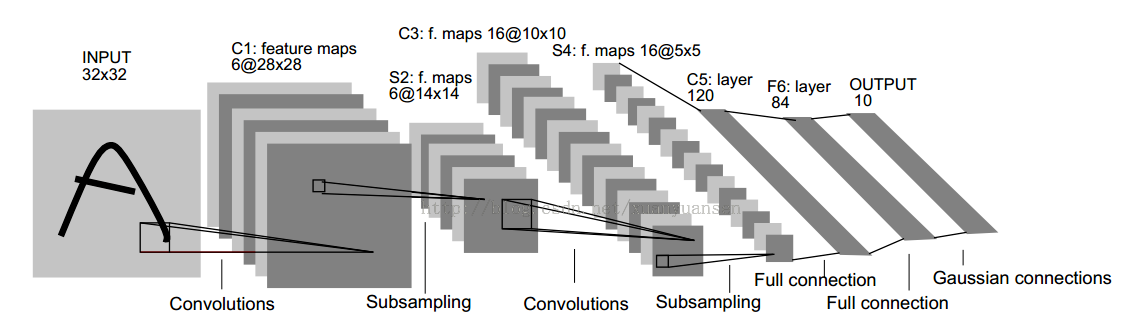
\includegraphics[width=1.0\linewidth]{intro_lenet.png}
\caption{LeNet-5~\cite{lecun1989backpropagation}网络结构。}
\label{fig:lenet}
\end{figure*}

以LeNet-5为例,如图~\ref{fig:lenet}所示,最基本的卷积神经网络包括六个重要的组成部分~\cite{gu2015recent,bengio2013representation,bengio2009learning,lecun2010convolutional,schmidhuber2015deep,Goodfellow-et-al-2016-Book}:卷积、池化、非线性激活函数、正则化、损失函数和网络训练方法。我们按照卷积神经网络的结构对近代卷积神经网络的研究进展进行简要的综述。

卷积层是卷积神经网络最基本的组成结构,具有局部特征提取的作用。对卷积层的改进主要体现在对卷积特征提取能力的增强,据我们了解有三种网络结构可以有效的提升卷积的特征表达能力。网络中的网络(Network in Network,NIN)~\cite{DBLP:journals/corr/LinCY13}是Lin等人在2013年提出的一种卷积层改进方法,传统的卷积层只能提取线性特征,Lin通过在传统卷积层中嵌入一个小型网络来增强局部感受野范围内特征的表达能力与非线性,进而提升整个NIN结构的拟合能力。最大输出单元(Maxout)~\cite{goodfellow2013maxout}是Goodfellow等人提出的,通过对多个卷积层的输出取最大的输出响应,来增强卷积层的非线性拟合能力。理论上,当卷积核足够大,具有两个隐层的Maxout可以以任意精度逼近任意连续曲线。Maxout采用线性分段函数来逼近复杂的非线性函数,确实可以提高网络的识别能力,但是需要引入大量的学习参数和计算量。Inception~\cite{szegedy2014going,szegedy2015rethinking,szegedy2016inception}是GoogLeNet的组成单元,它可以看做是对NIN的一种推广,Szegedy等人用不同大小的卷积核进行特征的提取,再从中优化出表达能力最强的一组特征。

池化是卷积神经网络另一个重要概念,它将位置相邻且语义相近的特征规约为一个特征,通过减小特征维度来降低网络的计算量,同时还可以保证特征具有一定程度的平移不变性。最常见的池化方法是均值池化(Average Pooling)和最大池化(Max Pooling)~\cite{weng1992cresceptron}。2007年,Hyvarinen等人~\cite{hyvarinen2007complex,bruna2013signal}受复杂细胞工作机制启发提出了$L_{p}$池化,通过对池化区域内的局部特征求取$p$范数来实现。均值池化和最大池化可以看成是$L_{p}$池化的两个特例,当 $p=1$ 时,$L_{p}$池化等价于均值池化;当 $p=\infty$ 时, $L_{p}$池化等价于最大池化。Yu等人~\cite{yu2014mixed}提出混合池化(Mixed Pooling)巧妙地将平均池化与最大池化进行结合,混合池化的输出响应是均值池化和最大池化的随机加权平均,随机的方式使得混合池化可以更有效地避免过拟合问题。受Dropout启发Zeiler和Fergus~\cite{zeiler2013stochastic}提出了随机池化(Stochastic Pooling)方法,根据多项式分布在池化区域内随机地选取激活值,随机池化也可以有效地避免过拟合问题。Rippel等人~\cite{rippel2015spectral}提出光谱池化(Spectral Pooling)方法,将卷积操作从时域转换到频域。与最大池化相比,具有线性低通滤波的光谱池化可以有效地减少池化过程中特征的信息损失。He等人~\cite{he2014spatial}提出了金字塔池化(Spatial Pyramid Pooling,SPP)用于提取多尺度的池化特征。与全局池化~\cite{DBLP:journals/corr/LinCY13}类似,金字塔池化可以提取固定长度的特征,使网络能够直接处理不同尺度的输入图像。Gong等人~\cite{gong2014multi}提出了多尺度无序池化(Multi-scale Orderless Pooling,MOP)来增强特征的不变形。

非线性激活函数可以增强卷积神经网络的非线性拟合能力,不同的激活函数形式,对网络的计算复杂度、拟合和泛化能力具有重要的影响。线性整流单元(Rectified Linear Unit,ReLU)~\cite{nair2010rectified}是目前卷积神经网络最常用的激活函数,ReLU是一个分段线性函数,在保留正的激活值的同时将负的激活值抑制为零。相对于传统的Sigmoid函数与双数正切函数,ReLU的计算更加简单快速,并且可以得到稀疏的特征表达。ReLU的缺点体现在梯度反向传播的过程中,对于未激活的神经元,ReLU的反向传播梯度为零,使得未激活的神经元无法进行参数更新。这对这个问题,Mass等人~\cite{maas2013rectifier}提出斜坡线性整流单元(Leaky Rectified Linear Unit,LReLU),通过对负数部分进行线性压缩来避免零梯度的产生。He等人~\cite{he2015delving}在LReLU中引入可学习的参数,提出了参数化线性整流单元(Parametric Rectified Linear Unit,PReLU),将LReLU中负数部分的斜坡压缩比率从固定值转变为一个可学习的参数,PReLU通过引入极少的参数,有效地提高了网络的拟合能力。对ReLU的另一项改进是Xu等人~\cite{xu2015empirical}提出的随机线性整流单元(Randomized Rectified Linear Unit,RReLU),负数部分的斜坡压缩比率通过在均匀分布上随机采样来生成,该方法同样通过引入随机机制在一定程度上避免了过拟合问题。Clevert等人~\cite{clevert2015fast}提出了指数线性单元(Exponential Linear Unit,ELU),可以在加速网络训练的同时,提高网络的识别率。相比于LReLU、PReLU和RReLU,ELU在负数部分引入了饱和机制,可以加快网络的学习速度。此外,最大化输出单元(Maxout)~\cite{goodfellow2013maxout}和概率最大化输出单元(Probout)~\cite{springenberg2013improving}也可以看做是对激活函数的一种改进方法。

损失函数反映了估计值与真值之间的误差,不同类型的损失函数反映了对问题的不同定义。在多类别物体分类问题中,最常用的损失函数是Softmax和多项式逻辑损失函数(Multinomial Logistic Loss)的一种结合形式。首先采用Softmax:${\hat{p}}_{n,k}=e^{x_n,k}/\sum_{k'=1}^{K}e^{x_{n,k'}}$ 生成 $K$ 个类别上的预测概率 $({\hat{p}}_{n,1}, {\hat{p}}_{n,2}, \dots{\hat{p}}_{n,K})$,再由预测概率来计算多元逻辑回归损失。信息增益损失函数(Information Gain Loss)是多项式逻辑损失函数的一种推广,信息熵是对信息的一种量化,信息增益表示在某种特定条件下的信息熵与原信息熵的差值,信息增益损失函数常用于文本分类中,多项式逻辑损失函数可以看成是信息增益损失函数的一种特殊形式。交叉熵损失函数(Cross Entropy Loss)常被用于知识蒸馏(Distilling Knowledge)~\cite{hinton2015distilling}等相关方法,经常与Sigmoid函数配合使用,加快网络参数的更新。另外一个常用的损失函数是铰链损失函数(Hinge Loss),也是支持向量机(SVM)中采用的损失函数。对比损失函数(Contrastive Loss)常用于双胞胎网络(Siamese Network)~\cite{chopra2005learning},用来量化一组数据对是否属于同一类。

正则化方法可以有效地抑制过拟合现象。Dropout是Hinton等人~\cite{hinton2012improving}首次提出的防止网络过拟合的正则化方法,通过随机地抑制网络一部分激活值,对输出结果进行正则化。Dropout可以防止网络在分类过程中过多地依赖于一个或一小部分神经元,使网络可以在丢失一部分信息的情况下依然作出正确的预测。此外,Dropout也可以理解过一种模型平均技术。自Dropout提出以来,出现了很多改进版本,Wang等人~\cite{wang2013fast}提出快速Dropout方法,采用高斯估计来取代蒙特卡洛采样,来提高网络的训练速度。Ba等人~\cite{ba2013adaptive}提出自适应Dropout方法,使隐层变量的Dropout比率可以通过一个与原网络参数共享的置信网络学习得到。Tompson等人~\cite{tompson2015efficient}发现,对于 $1{\times}1$ 的卷积层进行Dropout并不能有效地防止过拟合问题,因此他们提出了SpatialDropout方法来解决 $1{\times}1$ 卷积层的Dropout问题。DropConnect也是受Dropout启发的一种防止网络过拟合的有效方法,与Dropout不同的是,DropConnect通过随机抑制网络的连接权来实现正则化。此外,局部响应正则化(Local Response Normalization,LRN)通过引入特征间的竞争来实现正则化的效果,通过让激活值在多个通道的局部区域相互竞争,来实现正则化的目的。批正则化(Batch Normalization,BN)~\cite{ioffe2015batch}是Ioffe等人提出,批正则化以批为单位对特征的均值和方差进行估计,用估计的均值和方差对特征进行零均值标准化,通过对输出特征进行约束来实现正则化的目的。


对于卷积神经网络的训练,主要涉及参数的初始化与参数更新方法两个方面。卷积神经网络具有大量的参数,一组好的初始化参数可以加快网络的收敛,Krizhevsky等人~\cite{krizhevsky2012imagenet}采用一个均值为 0 标准差为 0.01 的高斯函数对参数进行随机初始化。Glorot等人~\cite{glorot2010understanding}提出Xavier方法对高斯初始化进行了改进,通过网络输入输出神经元的个数,来调整网络参数初始化的幅度,即采用一个以 0 为均值 $2/(n_{in}+n_{out})$ 为标准差的高斯函数对网络参数进行初始化,其中 $n_{in}$ 和 $n_{out}$ 分别是输入和输出神经元的个数。He等人~\cite{he2015delving}在Xavier基础上,进一步考虑了ReLU非线性激活函数对网络参数初始化的影响,对Xavier进行改进,使改良后的Xavier适用于初始化极深的卷积神经网络并且可以保证参数快速收敛。最常见的网络参数更新方法是随机梯度下降法(Stochastic Gradient Descent,SGD)~\cite{bottou2012stochastic},它是其他参数更新方法的基础。2011年,Duchi等人~\cite{duchi2011adaptive}提出自适应梯度法(Adaptive Gradient),通过融合梯度更新的历史信息来加快网络的收敛速度。2012年,Zeiler~\cite{zeiler2012adadelta}提出了AdaDelta方法,用于自适应地调节网络的学习率,使网络参数的更新更加鲁棒。同年,Tieleman和Hinton~\cite{tieleman2012}在Coursera公开课的讲义上提出RMSprop方法,可以自适应地更新网络的学习步长。2013年,Sutskever等人~\cite{sutskever2013importance}将NAG方法成功地应用于深层网络的训练,取得了更快的网络收敛速度。2015年,Kingma等人~\cite{kingma2014adam}提出了Adam方法,对动量因子进行自适应参数估计。2016年,谷歌深度思维团队提出了网络分解训练(Decoupled Neural Interfaces,DNI)~\cite{jaderberg2016decoupled},来解决网络在没有回传梯度的情况下的参数更新问题。网络分解训练通过梯度合成的方法,来预测当前层的回传梯度,打破了传统梯度下降法先前传再反传的限制,实现参数的异步更新。

%\begin{eqnarray} \label{equ:sgd}
%V_{t+1}&=&{\mu}V_t-{\alpha}{\nabla}\mathcal{L}(W_t)\nonumber\\
%W_{t+1}&=&W_t+V_{t+1}
%\end{eqnarray}
%其中 $W$ 是网络参数;$\mathcal{L}$ 是损失函数;$\alpha$ 是学习率;$\mu$ 是动量因子(Momentum)。Zeiler~\cite{zeiler2012adadelta}对SGD进行改进,使网络学习率的更新更加鲁棒,提出了AdaDelta参数更新方法:


%近年来对神经网络的研究,主要可以分为三个流派,分别是:基于概率模型的神经网络模型,基于数据或特征重构的自动编码器,和目前最受关注的卷积神经网络。


%从概率模型观点出发,特征学习的过程可以理解为,通过对大量输入数据的观察,找到一组可以正确表示输入数据样本分布的隐层特征。对于隐层特征$h$和观测数据$x$,对$h$和$x$的联合概率分布$p(x,h)$进行建模。特征提取的过程可以看成在已知输入数据$x$的情况下,预测隐层随机变量$h$概率分布的过程,即求解后验概率分布$p(h|x)$。学习的过程可以看做是采用极大似然估计的方法,对模型参数求解的过程。概率图模型采用图结构来描述随机变量之间的依赖关系,可以分为有向概率图和无向概率图两类。它们的区别仅仅体现在联合概率的定义,但两者学习的过程和计算量却截然不同。

%有向概率图模型可以统一解释为,在已知条件概率分布$p(x|h)$和先验概率分布$p(h)$的情况下,重构联合概率$p(x,h)=p(x|h)p(h)$的过程。基于有向概率图模型的网络包括:概率主成分分析(Probabilistic Principal Component Analysis ,PPCA)~\cite{tipping1999probabilistic}、概率解释的稀疏编码~\cite{olshausen1996emergence}、Sigmoid信念网络(Sigmoid Belief Networks)~\cite{neal1992connectionist}和深度信念网络(Deep Belief Network、DBN)~\cite{hinton2006reducing}。其中概率主成分分析和概率解释的稀疏编码常常被当做深度学习发展过程中的浅层学习网络。在概率主成分分析中,假设预测数据$x$是由隐层随机变量$h$生成的,并且隐层变量$h$和条件概率$p(x|h)$均服从高斯分布:
%\begin{eqnarray} \label{equ:ppca}
%p(h)&=&\mathit{N}(h|0,\sigma_{h}^{2}\mathit{I})\nonumber\\
%p(x|h)&=&\mathit{N}(x|Wh+\mu_x,\sigma_{x}^{2}\mathit{I})
%\end{eqnarray}
%概率解释的稀疏编码与此类似,但是隐层随机变量$h$不再服从高斯分布,而是服从稀疏诱导的拉普拉斯先验(Sparsity Inducing Laplace prior):
%\begin{eqnarray} \label{equ:psc}
%p(h)&=&\prod_{i}^{d_h}exp(-{\lambda}{\lvert}h_i{\rvert})\nonumber\\
%p(x|h)&=&\mathit{N}(x|Wh+\mu_x,\sigma_{x}^{2}\mathit{I})
%\end{eqnarray}
%借鉴于视觉皮层对复杂刺激的响应方式,Olshausen指出,经稀疏编码提取的图像基函数类似于生物视觉皮层V1区简单细胞的响应特性:局限性、方向性和选择性。

%无向概率图模型,即马尔科夫随机场(Markov Random Fields,MRFs),其联合概率$p(x,h)$可以表示为:
%\begin{eqnarray} \label{equ:mrf}
%p(x,h)=\frac{1}{Z_\theta}{\prod_i\psi_i(x)}{\prod_j\eta_j(h)}{\prod_k\upsilon_k(x,h)}
%\end{eqnarray}
%其中$\psi_i(x)$,$\eta_j(h)$和$\upsilon_k(x,h)$分别表示观测数据$x$,隐随机变量$h$和它们之间相互作用的群势能(Clique Potentials);$Z_\theta$为归一化因子。玻尔兹曼机(Boltzmann)~\cite{hinton1983optimal}是MRFs的一种简化形式,可以表示:
%\begin{eqnarray} \label{equ:bz}
%p(x,h)=\frac{1}{Z_\theta}exp(-\varepsilon_\theta(x,h))
%\end{eqnarray}
%其中$\varepsilon_\theta(x,h)$是能量函数;$\theta$是模型的参数。波尔兹曼机的能量通常定义为:
%\begin{eqnarray} \label{equ:bm_e}
%\varepsilon_\theta(x,h)^{BM}=-\frac{1}{2}x^{T}Ux-\frac{1}{2}h^{T}Vh-x^{T}Wh-b^{T}x-d^{T}h
%\end{eqnarray}
%其中参数$\theta=(U,V,W,b,d)$是模型的参数,分别代表观测层对观测层、隐层对隐层、观测层对隐层、观测层自身和隐层自身的连接关系。受限波尔兹曼机(Restricted Boltzmann Machine,RBM)是对波尔兹曼机的一种简化,也是最常见得波尔兹曼机计算模型。RBM的能量函数$\varepsilon_\theta(x,h)^{RBM}$仅仅是令$\varepsilon_\theta(x,h)^{BM}$中的$U=0, V=0$。与RBM相关的研究主要集中于模型的改进与学习算法两个方向。在模型方面,包括高斯受限玻尔兹曼机(GRBM)~\cite{krizhevsky2009learning}、均值方差受限玻尔兹曼机(mcRBM)~\cite{hinton2010modeling}、mPoT模型~\cite{mnih2010generating}、钉板(Spike-and-Slab)受限玻尔兹曼机(ssRBM)~\cite{courville2011spike}和深度玻尔兹曼机(Deep Boltzmann Machine、DBM)。在学习方法上包括吉布斯采样法(Gibbs Sampling)~\cite{hinton1983optimal}、对比离差算法(Contrastive Divergence,CD)~\cite{hinton1999products,hinton2006fast}、随机最大似然法(Stochastic Maximum Likelihood、SML)~\cite{younes1999convergence}、快速持续对比离差算法(Fast-weights Persistent Contrastive Divergence,FPCD)~\cite{tieleman2009using}。
%
%
%概率模型的学习需要求隐随机变量相对于观测变量的后验概率,不论在有向图模型还是无向图模型,后验概率的计算是很复杂甚至于无法计算的,尤其是对于深层网络结构。因此通常采用采样的方法对其进行估计,这往往会引入估计误差。自动编码器(Autoencoders)~\cite{bourlard1988auto,hinton1994autoencoders}是一种直接对数据数据进行重构的特征提取方法,包括编码(encoder)和解码(decoder)两个过程,将编码和解码函数分别记为$f_\theta$和$g_\theta$,其中$\theta$是需要学习的参数。一个最基本的自动编码器可以通过最小化重构误差函数求解:
%\begin{eqnarray} \label{equ:ae}
%\mathcal{J}_{AE}(\theta)=\sum_{t}L(x^{(t)},g_{\theta}(f_{\theta}(x^{(t)})))
%\end{eqnarray}
%其中$x^{(t)}$是训练样本;$L$为L1或L2范数。与自动编码器相关的研究主要包括稀疏自动编码器(Sparse Autoencoders,SAE)~\cite{poultney2006efficient}、去噪自动编码器(Denoising Autoencoders,DAE)~\cite{vincent2008extracting}收缩自动编码器(Contractive Autoencoders,CAE)~\cite{rifai2011contractive}预测自动编码器(Predictive Sparse Decomposition,PSD)~\cite{olshausen1996emergence}等,这些方法的主要区别在于优化函数有所不同:
%\begin{eqnarray} \label{equ:aes}
%\mathcal{J}_{SAE}(\theta)&=&\sum_{t}L(x^{(t)},g_{\theta}(f_{\theta}(x^{(t)})))+\lambda\sum_{t}\lVert{h^{(t)}}\lVert_{1}\nonumber\\
%\mathcal{J}_{DAE}(\theta)&=&\sum_{t}\mathbb{E}_{q(\tilde{x}|x^{(t)})}[L(x^{(t)},g_{\theta}(f_{\theta}(x^{(t)})))]\nonumber\\
%%\mathcal{J}_{CAE}(\theta)&=&\sum_{t}L(x^{(t)},g_{\theta}(f_{\theta}(x^{(t)})))+\lambda\vert\vert{f_{\theta}(x)_j(1-f_{\theta}(x)_j)W_j}\vert\vert_{F}^{2}
%\mathcal{J}_{CAE}(\theta)&=&\sum_{t}L(x^{(t)},g_{\theta}(f_{\theta}(x^{(t)})))+\lambda\lVert{\frac{\partial{f_\theta}}{\partial{x}}(x)}\rVert_{F}^{2}\nonumber\\
%\mathcal{J}_{PSD}&=&\sum_{t}\lVert{h^{(t)}}\lVert_{1}+\lVert{x^{(t)}-Wh^{(t)}}\lVert_{2}^{2}+\lVert{h^{(t)}-f_{\alpha}(x^{(t)})}\lVert_{2}^{2}
%\end{eqnarray}
%
%
%深度学习的另外一个分支卷积神经网络是受生物视觉皮层认知机制启发而来。1959年,Hubel和Wiesel~\cite{hubel1959receptive,hubel1962receptive}在生物视觉皮层的早期研究中,发现了在感受野范围内视觉皮层中简单细胞、复杂细胞和超复杂细胞对光信号具有不同的响应。受此启发,日本学者Fukushima提出了认知机(Cognitron)~\cite{fukushima1975cognitron} 和神经认知机(Neocognitron)~\cite{fukushima1980neocognitron}的计算模型,通常被认识是最早卷积神经网络模型。1989年,LeCun等人~\cite{lecun1989backpropagation,le1990handwritten}将误差反向传播算法引入到神经认知机模型中,提出了著名的LeNet-5网络,如图~\ref{fig:lenet}所示,奠定了现代卷积神经网络的计算框架。但由于当时训练数据规模和计算性能上的限制,卷积神经网络并没有受到广泛的关注。
%
%2012年,Krizhevsky等人~\cite{krizhevsky2012imagenet}提出了一个与LeNet-5类似,但结构更深的卷积神经网络模型AlexNet,借助于高性能的GPU并行计算能力,在2012年ImageNet大规模视觉识别比赛(ImageNet Large Scale Visual Recognition Competition,ILSVRC)中一举夺冠,掀起了卷积神经网络的研究热潮。此后,各种网络模型如ZFNet~\cite{zeiler2014visualizing},VGGNet~\cite{simonyan2014very},GoogleNet~\cite{szegedy2014going,szegedy2015rethinking,szegedy2016inception}、ResNet~\cite{he2015deep}等被相继提出,用以解决计算机视觉问题。



%
%\begin{figure*}
%\centering
%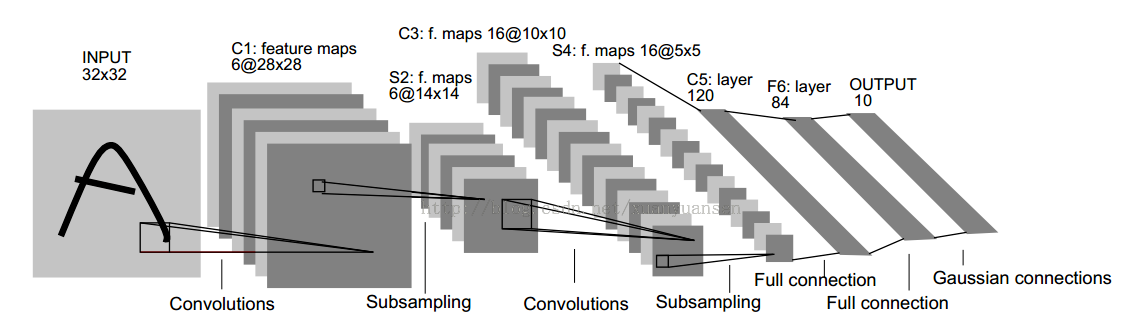
\includegraphics[width=1.0\linewidth]{intro_lenet.png}
%\caption{LeNet-5~\cite{lecun1989backpropagation}网络结构。}
%\label{fig:lenet}
%\end{figure*}
%
%以LeNet-5为例如图~\ref{fig:lenet}所示,最基本的卷积神经网络包括六个重要的组成部分~\cite{gu2015recent}:卷积、池化、非线性激活函数、正则化、损失函数和网络训练。下面我们将分别介绍卷积神经网络各部分的改进。
%
%卷积层是卷积神经网络最基本的组成结构,主要用于特征提取。对卷积层的改进主要体现在对特征提取能力的增强,据我们了解有三种网络结构可以有效的提升特征表达能力。网络中的网络(Network in Network,NIN)~\cite{DBLP:journals/corr/LinCY13}是Lin等人提出的,传统的卷积层只能提取线性特征,Lin通过在传统卷积层中嵌入一个小型网络来特征卷积层的逼近能力。最大输出单元(Maxout)~\cite{goodfellow2013maxout}是Goodfellow等人提出的,通过对多个卷积层的输出求最大的方式,来增强卷积层的拟合能力。理论上,当卷积核足够大时两个隐层的Maxout可以以任意精度逼近任意曲线。Inception~\cite{szegedy2014going,szegedy2015rethinking,szegedy2016inception}可以看做是对NIN的推广,Szegedy等人用不同大小的卷积核提取出不同形式的特征,再从中优化出表达能力最强的一组特征。
%
%池化是卷积神经网络的一个重要概念,它可以通过减小特征维度从而降低网络的计算量,同时可以使得特征具有一定的平移不变性。最长见的池化方法是均值池化(Average Pooling)和最大池化(Max Pooling)~\cite{weng1992cresceptron}。$L_{p}$池化~\cite{hyvarinen2007complex,bruna2013signal}是受复杂细胞工作机制启发的一种池化方法,$L_{p}$池化可以表示为:
%\begin{eqnarray} \label{equ:lp}
%h_{i,j,k}=[\sum_{(m,n)\in{\mathcal{R}_{ij}}}(x_{m,n,k})^p]^{1/p}
%\end{eqnarray}
%其中 $h_{i,j,k}$ 表示第 $k$ 个通道上位置 $(i,j)$ 处池化输出;$x_{m,n,k}$ 表示 $(m,n)\in\mathcal{R}_{i,j}$ 位置上特征值;$\mathcal{R}_{i,j}$代表位置 $(i,j)$ 的池化区域。当 $p=1$ 时,$L_{p}$池化等价于均值池化;当 $p=\infty$ 时, $L_{p}$池化等价于最大池化。Yu等人~\cite{yu2014mixed}采用混合池化(Mixed Pooling)巧妙地将平均池化与最大池化有效结合,混合池化可以表示为:
%\begin{eqnarray} \label{equ:mp}
%h_{i,j,k}={\lambda}{\max_{(m,n)\in\mathcal{R}_{i,j}}x_{m,n,k}}+(1-\lambda)\frac{1}{|\mathcal{R}_{i,j}|}{\sum_{(m,n)\in\mathcal{R}_{i,j}}x_{m,n,k}}
%\end{eqnarray}
%其中 $\lambda$ 是一个在 0 或 1 之间取值的随机数。受Dropout启发Zeiler和Fergus~\cite{zeiler2013stochastic}提出了随机池化(Stochastic pooling)方法,可以通过随机操作防止过拟合。Rippel等人~\cite{rippel2015spectral}提出光谱池化(Spectral Pooling)方法,通过将卷积操作从时域转换到频域,可以有效地减少池化过程中特征信息损失的问题。He等人~\cite{he2014spatial}提出了金字塔池化(Spatial Pyramid Pooling,SPP)用于提出固定长度的特征,是对~\cite{DBLP:journals/corr/LinCY13}中全局池化的一种推广。Gong等人~\cite{gong2014multi}提出了多尺度无序池化(Multi-scale Orderless Pooling ,MOP)来增强特征的不变形。
%
%非线性激活函数可以增强卷积神经网络的非线性拟合能力,不同的激活函数形式,对网络的计算量、拟合和泛化能力具有重要的影响。线性整流单元(Rectified linear unit,ReLU)~\cite{nair2010rectified}是目前卷积神经网络最常用的激活函数,ReLU可以表示为:
%\begin{eqnarray} \label{equ:relu}
%h_{i,j,k}=\max(x_{i,j,k},0)
%\end{eqnarray}
%其中$x_{i,j,k}$表示第 $k$ 个通道位置 $(i,j)$ 处的输入特征。相对于传统的Sigmoid函数:
%\begin{eqnarray} \label{equ:sigmoid}
%h_{i,j,k}=\frac{1}{1+e^{-x_{i,j,k}}}
%\end{eqnarray}
%和双曲正切函数:
%\begin{eqnarray} \label{equ:tanh}
%h_{i,j,k}=\frac{e^{x_{i,j,k}}-e^{-x_{i,j,k}}}{e^{x_{i,j,k}}+e^{-x_{i,j,k}}}
%\end{eqnarray}
%ReLU的计算更简单,并且可以得到稀疏的特征表示。但是对于未激活的神经元,ReLU的反向传播梯度为0,使得未激活的神经元无法进行参数更新。Mass等人~\cite{maas2013rectifier}提出斜坡线性整流单元(Leaky Rectified linear unit,LReLU)来解决这个问题,计算公式如下:
%\begin{eqnarray} \label{equ:lrelu}
%h_{i,j,k}=\max(x_{i,j,k},0)+{\lambda}\min(x_{i,j,k},0)
%\end{eqnarray}
%其中$\lambda$是一个预定义的取值在 $(0,1)$ 之间的随机变量。He等人~\cite{he2015delving}对LReLU进一步改进,提出了参数化线性整流单元(Parametric Rectified linear unit,PReLU),PReLU可以表示为:
%\begin{eqnarray} \label{equ:prelu}
%h_{i,j,k}=\max(x_{i,j,k},0)+{\lambda}_k\min(x_{i,j,k},0)
%\end{eqnarray}
%其中 ${\lambda}_k$ 是第 $k$ 个通道上的可学习参数。PReLU通过引入极少的参数,有效地提高了网络的拟合能力。对LReLU的另一项改进是Xu等人~\cite{xu2015empirical}提出的随机线性整流单元(Randomized Rectified linear unit,ReLU),与公式~\ref{equ:prelu}具有相同的形式,但是其中的 ${\lambda}_k$ 服从均匀分布,前向传播过程中通过随机采样产生。Clevert等人~\cite{clevert2015fast}提出了指数线性单元(Exponential Linear Unit,ELU),可以在加速网络的训练的同时,提高网络的识别率,ELU可以表示为:
%\begin{eqnarray} \label{equ:elu}
%h_{i,j,k}=\max(x_{i,j,k},0)+\min({\lambda}(e^{z_{i,j,k}}-1),0)
%\end{eqnarray}
%其中 $\lambda$ 是一个预定义的加权因子。
%
%损失函数反映了估计值与真值之间的误差,不同类型的损失函数反映了对问题的不同定义。在多类别物体分类问题中,最常用的损失函数是Softmax和多项式逻辑损失函数(Multinomial Logistic Loss)结合的一种形式。首先采用Softmax:${\hat{p}}_{n,k}=e^{x_n,k}/\sum_{k'=1}^{K}e^{x_{n,k'}}$生成 $K$ 个类别上的预测概率 $({\hat{p}}_{n,1}, {\hat{p}}_{n,2}, \dots{\hat{p}}_{n,K})$,再通过预测概率计算多元逻辑回归损失:
%\begin{eqnarray} \label{equ:softmax}
%\mathcal{L}=-\frac{1}{N}[\sum_{n=1}^{N}\sum_{k=1}^{K}\delta\{l_{n}=k\}log{\hat{p}}_{n,k}]
%\end{eqnarray}
%其中 $N$ 代表样本总数;$l$ 是样本的正确标签,$\delta$ 是指示器函数。信息增益损失函数(Information Gain Loss)是多项式逻辑损失函数的一种推广,信息熵是对信息的一种量化,信息增益表示在某种特定条件下的信息熵与原信息熵的差值,信息增益损失函数常用于文本分类中,可以公式化描述为:
%\begin{eqnarray} \label{equ:information}
%\mathcal{L}=-\frac{1}{N}\sum_{n=1}^{N}\sum_{k=1}^{K}H_{l_n,k}log({\hat{p}}_{n,k})
%\end{eqnarray}
%其中 $H$ 是信息增益矩阵,当 $H=I$时,信息增益损失函数等价于多项式逻辑损失函数。交叉熵损失函数(Cross Entropy Loss)常被用于知识蒸馏(Distilling Knowledge)~\cite{hinton2015distilling}等相关方法中,经常与Sigmoid函数配合使用,加快网络的训练速度,交叉熵损失函数定义为:
%\begin{eqnarray} \label{equ:cross}
%\mathcal{L}=\frac{1}{N}\sum_{n=1}^{N}[p_n log{\hat{p}}_n+(1-p_n)log(1-{\hat{p}}_n)]
%\end{eqnarray}
%另外一个常用的损失函数是铰链损失函数(Hinge Loss),也是支持向量机(SVM)中采用的损失函数,定义为:
%\begin{eqnarray} \label{equ:hinge}
%\mathcal{L}=\frac{1}{N}\sum_{n=1}^{N}\sum_{k=1}^{K}[max(0,1-\delta\{l_n=k\}W^{T}x_{n})]^p
%\end{eqnarray}
%其中 $W$ 是分类器线性权重矩阵,$\delta$ 是一个映射到 $[-1,1]$ 的指示器函数;$p=1$ 表示 $L_1$ 范数,$p=2$ 表示 $L_2$ 范数。对比损失函数(Contrastive Loss)常用于双胞胎网络(Siamese Network)~\cite{chopra2005learning},用来量化一组数据对是否属于同一类,定义为:
%\begin{eqnarray} \label{equ:contrastive}
%\mathcal{L}=\frac{1}{2N}\sum_{n=1}^{N}\delta(l_n^{(a)}=l_n^{(b)})d^2+\delta(l_n^{(a)}\not{=}l_n^{(b)})max(margin-d,0)^2
%\end{eqnarray}
%其中 $d=||x_n^{(a)}-x_n^{(b)}||_2$ 代表 $a$ 和 $b$ 两个网络特征向量 $x_n$ 的欧氏距离。
%
%
%正则化方法可以有效地抑制过拟合现象。Dropout是Hinton等人~\cite{hinton2012improving}首次提出的防止网络过拟合的方法,通过随机地抑制网络一部分激活值,对输出结果进行正则化。此外,Dropout也可以理解过一种模型平均技术。自Dropout提出以来,出现了很多改进版本,例如快速Dropout方法~\cite{wang2013fast}、自适应Dropout方法~\cite{ba2013adaptive}和空间Dropout方法~\cite{tompson2015efficient}。DropConnect也是受Dropout启发的一种防止网络过拟合的有效方法,与Dropout不同的是,DropConnect通过随机抑制网络的连接权来实现正则化。局部响应正则化(Local Response Normalization,LRN)通过引入特征间的竞争来实现正则化的效果,LRN可以表示为:
%\begin{eqnarray} \label{equ:lrn}
%h_{i,j,k}=x_{i,j,k}/(k+{\alpha}\sum_{l=max(0,i-n/2)}^{min(N-1,i+n/2)}(x_{i,j,l})^{2})^{\beta}
%\end{eqnarray}
%其中$k,n,\alpha,\beta$是规则化的超参,通过让激活值在 $n$ 个通道内竞争,来实现正则化的目的。批正则化(Batch Normalization,BN)~\cite{ioffe2015batch}是Ioffe等人提出,通过对输出数据进行约束来实现正则化的目的,可以表示为:
%\begin{eqnarray} \label{equ:bn}
%\hat{x}_{i,j,k}&=&(x_{i,j,k}-\mu_{k})/\sqrt{(\delta_{k}^{2}+\epsilon)}\nonumber\\
%h_{i,j,k} &=& BN(x_{i,j,k}) = \gamma\hat{x}_{i,j,k}+\beta
%\end{eqnarray}
%其中 $\mu_{k}$ 和 $\delta_{k}$ 是每批养样本在通道 $k$ 上的均值与方差;$\gamma$ 和 $\beta$ 是可学习的参数,用于增强BN的特征表达能力。
%
%对于卷积神经网络的训练,主要涉及参数的初始化与更新方法。卷积神经网络具有大量的参数,一组好的初始化参数可以加快网络的收敛,Krizhevsky等人~\cite{krizhevsky2012imagenet}采用一个均值为 0 标准差为 0.01 的高斯函数对参数进行随机初始化。Glorot等人~\cite{glorot2010understanding}提出Xavier方法对高斯初始化进行了改进,通过网络输入输出神经元的个数,来调整网络参数初始化的幅度,即采用一个以 0 为均值 $2/(n_{in}+n_{out})$ 为标准差的高斯函数对网络参数进行初始化,其中 $n_{in}$ 和 $n_{out}$ 分别是输入和输出神经元的个数。He等人~\cite{he2015delving}在Xavier基础上,进一步考虑了ReLU非线性激活函数对网络参数初始化的影响,对Xavier进行改进,使其适用于初始化极深的卷积神经网络并可以快速收敛。最常见的网络参数更新方法是梯度下降法(Stochastic Gradient Descent,SGD)~\cite{bottou2012stochastic},可以表示为:
%\begin{eqnarray} \label{equ:sgd}
%V_{t+1}&=&{\mu}V_t-{\alpha}{\nabla}\mathcal{L}(W_t)\nonumber\\
%W_{t+1}&=&W_t+V_{t+1}
%\end{eqnarray}
%其中 $W$ 是网络参数;$\mathcal{L}$ 是损失函数;$\alpha$ 是学习率;$\mu$ 是动量因子(Momentum)。Zeiler~\cite{zeiler2012adadelta}对SGD进行改进,使网络学习率的更新更加鲁棒,提出了AdaDelta参数更新方法:
%\begin{eqnarray} \label{equ:sgd}
%(v_t)_i&=&\frac{RMS((v_{t-1})_i)}{RMS(\nabla\mathcal{L}(W_t))_i}(\nabla\mathcal{L}(W_t))_i\nonumber\\
%RMS(\nabla\mathcal{L}(W_t))_i&=&\sqrt{E[g^2]+\epsilon}\nonumber\\
%E[g^2]_t&=&{\delta}E[g^2]_{t-1}+(1-\delta)g_{t}^2\nonumber\\
%(W_{t+1})_i&=&(W_t)_i-\alpha(v_t)_i
%\end{eqnarray}
%此外,自适应梯度法(Adaptive Gradient)~\cite{duchi2011adaptive}、Adam法~\cite{kingma2014adam}、Nesterov梯度法~\cite{sutskever2013importance}、RMSProp等都是基于梯度下降的改进方法。2016年,谷歌DeepMind提出了网络分解训练(Decoupled Neural Interfaces,DNI)~\cite{jaderberg2016decoupled},来解决在网络没有回传梯度的情况下,参数的更新问题。网络分解训练通过梯度合成的方法,来预测当前层的梯度,打破了传统梯度下降法先前传再反传的限制,实现参数的异步更新。
%
%此外,卷积神经网络在语音识别(Speech Recognition)、信号处理(Signal Processing)、物体检测与识别(Object Detection and Recognition)、文本的检测与识别(Text Detection and Recognition)、多任务迁移学习(Multitask and Transfer Learning)等诸多领域都取得了重大的创新与突破。

\section{预备知识}

卷积神经网络是一种特殊的神经网络结构,它采用卷积操作代替了神经网络中矩阵乘法操作。本节是与卷积神经网络相关的预备知识,主要介绍了卷积神经网络的卷积操作,讨论了卷积操作的动机与优势,最后介绍了卷积神经网络的另外两个重要组成池化和非线性化。

\begin{figure}[h]
\centering
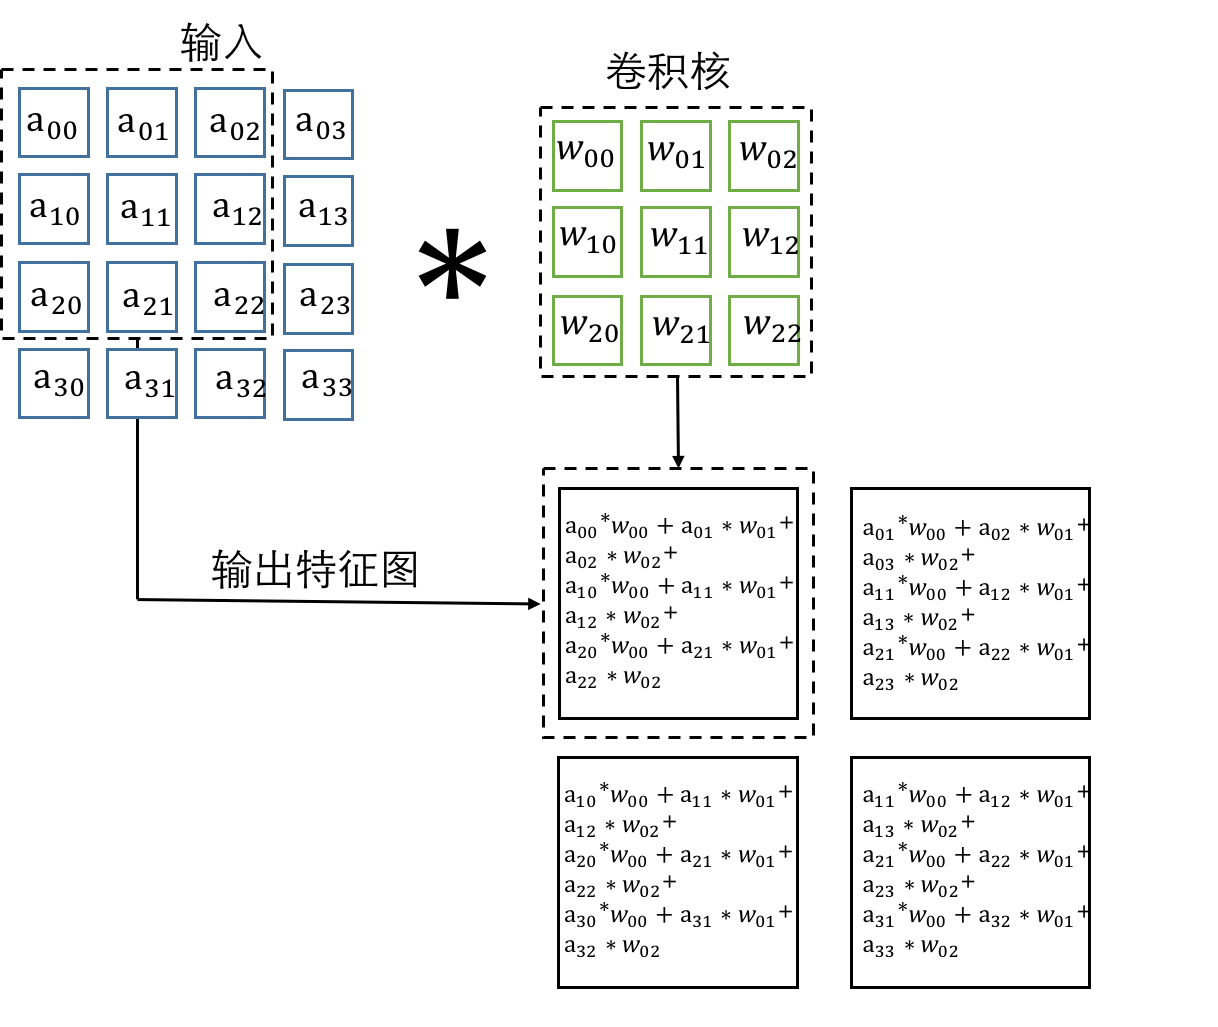
\includegraphics[width=1\linewidth]{intro_conv.png}
\caption{卷积神经网络的卷积操作实现方式。传统的卷积操作需要对卷积核进行反转,使卷积具有交换律。在卷积神经网络中,交换律并不重要,卷积网络通过端到端学习的方式,可以学习到一组位置相关的卷积核参数,是否对卷积核进行反转不会影响卷积的输出结果。本文沿用了大多数卷积神经网络库函数中卷积操作的实现方式。}
\label{fig:intro_conv}
\end{figure}

为了引出卷积神经网络中卷积操作的定义,我们首先分析在最一般的形式中,两个函数的卷积操作定义。假设我们正在使用一个雷达设备对一个物体进行跟踪,雷达设备给出了一个输出序列 $x(t)$,表示物体在 $t$ 时刻的位置。这里 $x$ 和 $t$ 都是实数,在不同的时刻 $t$ 我们可以得到一个不同的观测位置 $x(t)$。因为雷达的输出具有噪声,为了较小噪声对物体测距的影响,我们希望通过多次测量求均值的方式来减弱噪声影响。当然,当前时刻的观测值与物体的真实位置最为相关,因此我们希望在加权平均的过程中,对当前时刻的观测值赋予更高的权重。通过使用一个加权函数 $w(t)$ 来实现这样的目的,其中 $t$ 代表测量的有效时间。每一个时刻我们均采用这用加权平均的方式对观测物体的位置进行平滑,则得到一个新的函数 $s(t)$ ,表示 $t$ 时刻平滑后的观测物体位置,如公式(~\ref{equ:convolution1})所示:
\begin{eqnarray} \label{equ:convolution1}
s(t)=\int{x(a)w(t-a)da}
\end{eqnarray}
这个操作即为两个函数的卷积操作,卷积通常可以记为星号乘法运算:
\begin{eqnarray} \label{equ:convolution2}
s(t)=(x*w)(t)
\end{eqnarray}
在上述例子中,$w$ 是一个概率密度函数,并且对于负的时间序列,$w$ 需要置为零。实际上,这些限制仅仅针对于上述雷达测距的例子,通常来讲,卷积可以定义在满足公式 (\ref{equ:convolution1})的任意函数上,可以用来表示除加权平均之外的其他含义。在上述例子中,我们假设雷达的观测是一个与时间相关的连续函数,但是计算机可以处理的数据往往是离散的。如果我们假设 $x(t)$ 和 $w(t)$ 是定义在正整数集合 $t$ 上的离散函数,上述卷积操作可以表示为:
\begin{eqnarray} \label{equ:convolution3}
s(t)=(x*w)(t)=\sum_{a=-\infty}^{\infty}x(a)w(t-a)
\end{eqnarray}

在卷积神经网络中,上述例子中的 $x$ 通常表示输入,函数 $w$ 用于表示特征核,输出 $s$ 称为特征图。卷积神经网络的输入、特征核和输出特征图均是多维矩阵,对于输入是二维图像的情况下,卷积操作可以表示为:
\begin{eqnarray} \label{equ:c1}
s(i,j)=(I*K)(i,j)=\sum_{m}\sum_{n}I(m,n)K(i-m,j-n)
\end{eqnarray}
卷积操作满足交换律,因此我们可以将图像的卷积表示成一种更为直观的方式:
\begin{eqnarray} \label{equ:c2}
s(i,j)=(I*K)(i,j)=\sum_{m}\sum_{n}I(i-m,j-n)K(m,n)
\end{eqnarray}

卷积操作满足交换律是因为我们对卷积核进行了反转,公式(\ref{equ:c1})中,随着 $m$ 的增大,输入图像的索引随之增大,但是卷积核的索引随之减小。但是这样的性质在卷积神经网络并不是必要的,因此在很多卷积神经网络相关的库函数中,采用一种与图像卷积相似但不具有特征核反转的卷积操作:
\begin{eqnarray} \label{equ:c3}
s(i,j)=(I*K)(i,j)=\int_{m}\int_{n}I(i+m,j+n)K(m,n)
\end{eqnarray}


在很多机器学习相关的库函数中,均采用公式(\ref{equ:c3})的卷积实现方式,本文我们沿用这样的表示方法。实际上,是否对卷积核进行反转对卷积的结果并没有太大的影响,网络端到端的学习方法,可以学习到一组位置相关的卷积核参数。图~\ref{fig:intro_conv} 是公式(\ref{equ:c3})所描述的一个卷积操作示例,对于输入为 $4\times4$ 像素大小的输入图像,采用 $3\times3$ 感受野大小的卷积核对其进行卷积,在步长为 1 且没有边界扩充的情况先,输出了一个 $2\times2$ 像素大小的特征图,特征图中每个位置的计算过程如图~\ref{fig:intro_conv} 所示。

卷积利用了三个重要思想来提高特征表达能力:稀疏表达、权值共享和平移同变性。此外,卷积神经网络还可以采用卷积堆叠的方式来实现更大范围的感受野,从而处理不同规模的输入图像。下面我们将分别介绍卷积操作的这三个主要特点。


\begin{figure}[h]
\centering
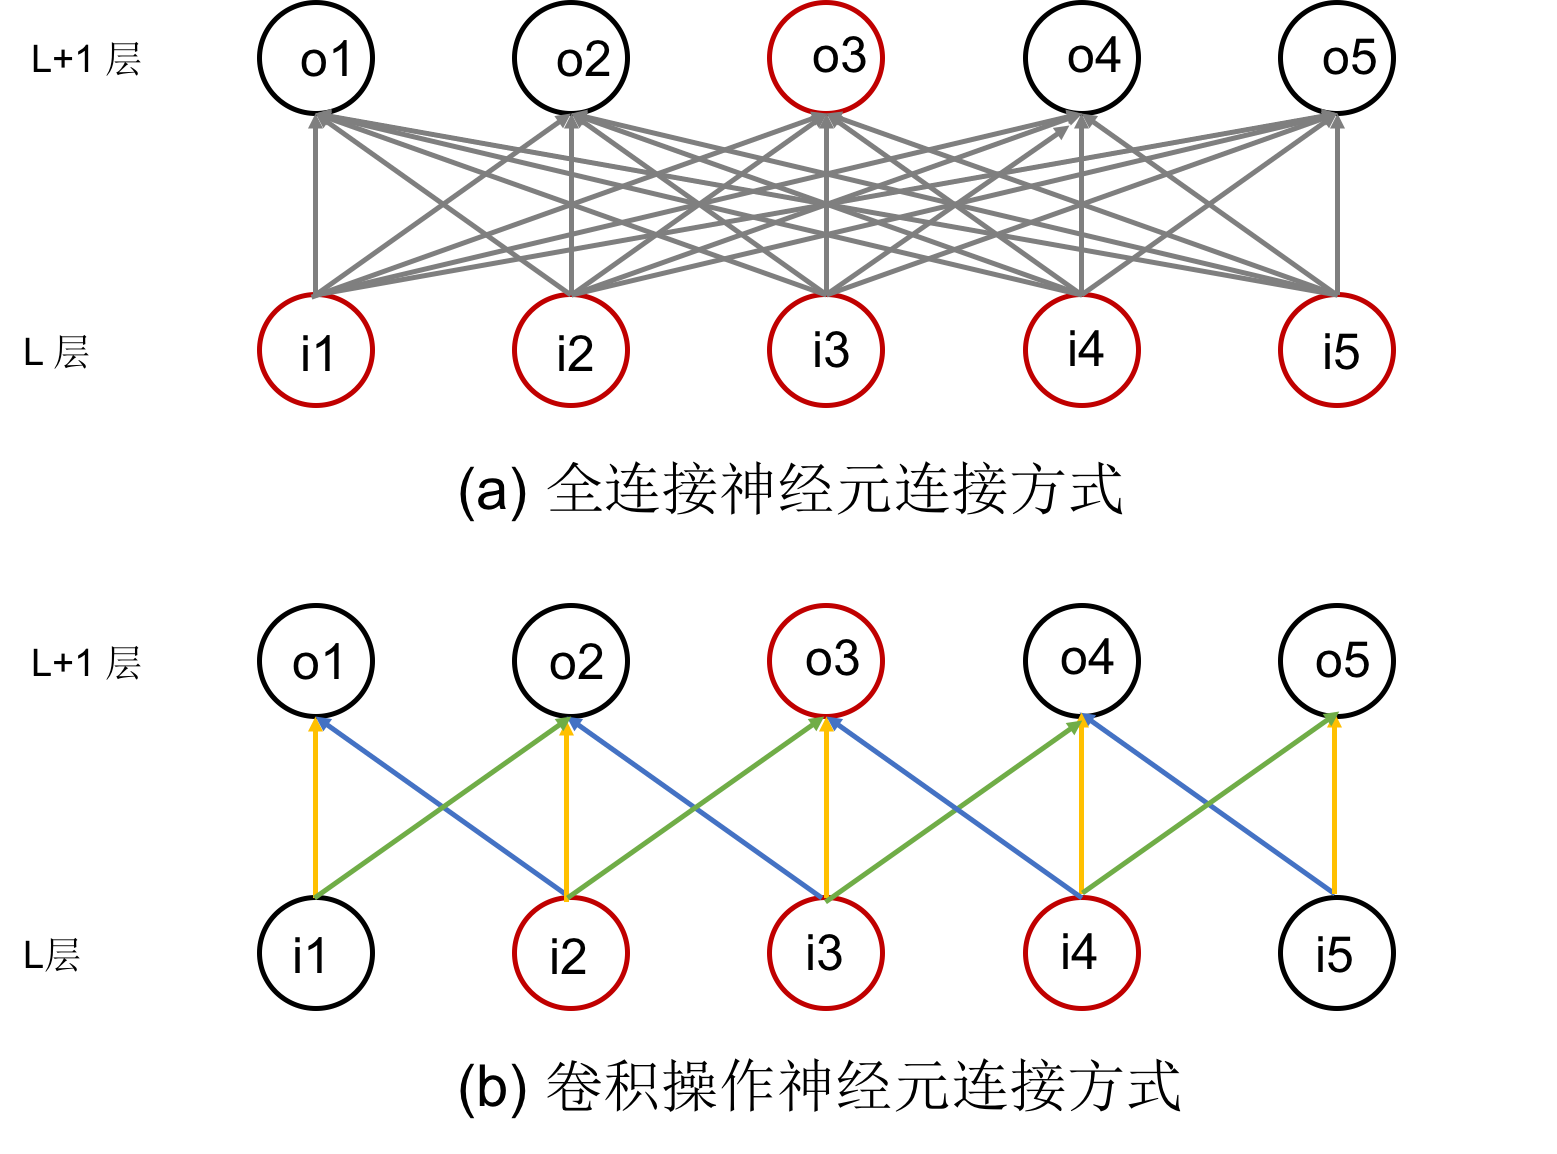
\includegraphics[width=0.8\linewidth]{intro_sparse.png}
\caption{稀疏连接与权值共享。对于图(a)中全连接神经元连接方式,对于高亮的输出神经元o3,所有的输入神经元i1,i2,i3,i4,i5均参与了全连接运算。对于图(b)中卷积操作神经元连接方式,对于高亮的输出神经元o3,与之位置相邻的三个输入神经元i2,i3,i4参与了卷积运算。即卷积操作相对于全连接具有稀疏连接的特性。卷积的权值共享,如图(b)所示,从输入到输出的连接权中,相同颜色的连线具有相同的权值参数。对于图中的例子,一共13条从输入到输出的连接权具有三种不同的颜色,即对应了三种不同的权重参数。举例来说,对于绿色的连接边,从i1到o2,从i2到o3,从i3到o4,从i4到o5,这四条边具有相同的参数,即权值共享。}
\label{fig:intro_sparse}
\end{figure}


传统的神经网络采用矩阵乘法来实现输入到输出的映射,对于每个输出单元都需要所有的输入神经元参与乘法运算。卷积神经网络采用稀疏连接(稀疏权重)的方式来实现特征提取,如图~\ref{fig:intro_conv}所示,特征核的大小远远小于输入图像的大小。对于一张具有成千上万个像素点的输入图像,卷积神经网络采用十几个或上百个像素的特征核就可以有效地提取图像的局部特征,例如颜色、边缘、角点等。这意味着卷积神经网络仅仅需要较少的参数,可以有效地较小模型参数,强化对图像局部特征的统计特性。此外,更少的卷积核参数意味着更少的乘法操作,对网络计算速度具有较大的提升。一个卷积稀疏连接的示例如图~\ref{fig:intro_sparse}所示。对于图~\ref{fig:intro_sparse}(a)中全连接神经元连接方式,对于高亮的输出神经元o3,所有的输入神经元i1,i2,i3,i4,i5均参与了全连接运算。对于图~\ref{fig:intro_sparse}(b)中卷积操作神经元连接方式,对于高亮的输出神经元o3,与之位置相邻的三个输入神经元i2,i3,i4参与了卷积运算。即卷积操作相对于全连接具有稀疏连接的特性。

尽管单层的卷积具有稀疏连接的特点,但是在深层的卷积神经网络结构中,卷积采用逐层堆叠的方式,使得深层的神经元可以间接地连接到多个输入单元,如图~\ref{fig:intro_rf}所示。如果L层代表输入图像,对于 $3\times3$ 感受野大小的卷积操作,L+1层的感受野大小为 $3\times3$,L+2层相对于L+1层具有 $3\times3$ 的感受野,但是相对于输出层L层,L+2层的感受野大小为 $5\times5$。尽管对于单层的卷积操作来说,从输入到输出神经元的连接具有稀疏的特点,但是多个卷积层的堆叠,使得深层神经元可以间接地作用于绝大部分甚至整张输入图像。这使得卷积神经网络可以通过多层卷积结构的堆叠来实现复杂的特征提取。

\begin{figure}
\centering
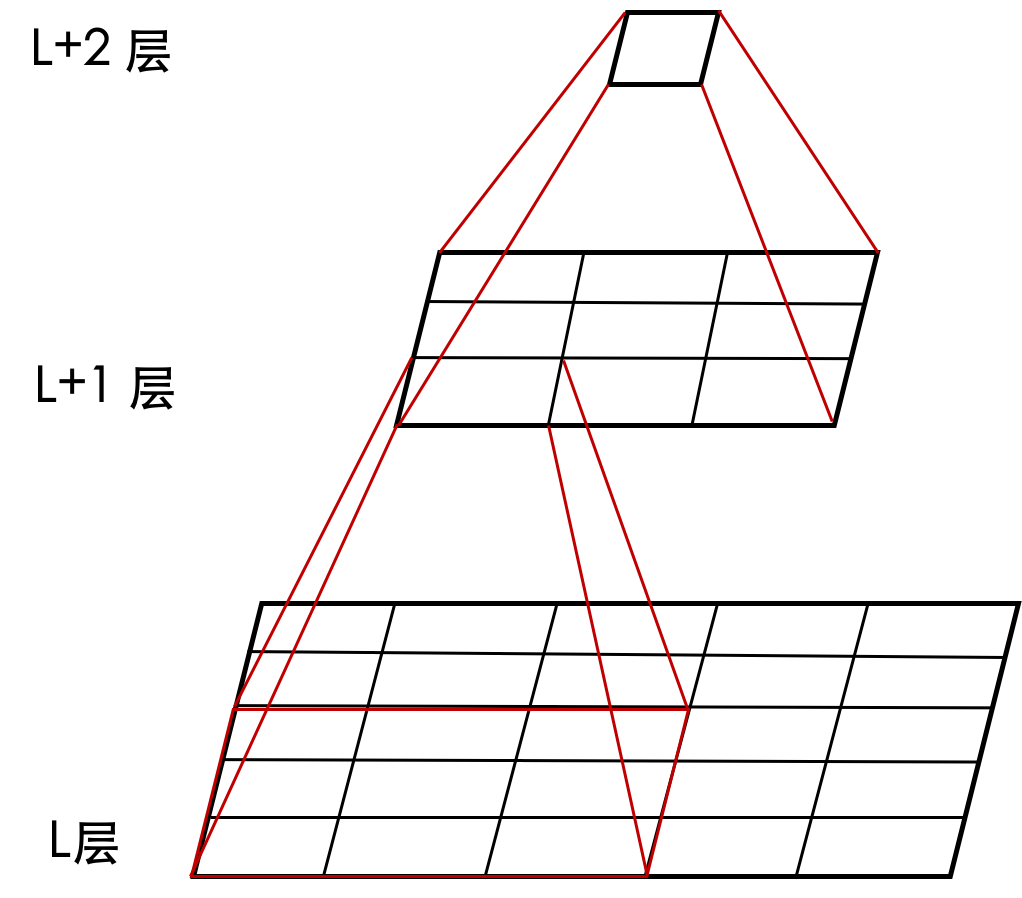
\includegraphics[width=0.7\linewidth]{intro_rf.png}
\caption{高层神经元的感受野。在深层卷积神经网络中,高层神经元的感受野范围大于浅层神经元的感受野,且随着深度的加深,感受野会逐渐增大。如图所示,如果L层代表输入图像,对于 $3\times3$ 感受野大小的卷积操作,L+1层的感受野大小为 $3\times3$,L+2层相对于L+1层具有 $3\times3$ 的感受野,但是相对于输出层L层,L+2层的感受野大小为 $5\times5$。尽管对于单层的卷积操作来说,从输入到输出神经元的连接具有稀疏的特点,但是多个卷积层的堆叠,使得深层神经元可以间接地作用于绝大部分甚至整张输入图像。}
\label{fig:intro_rf}
\end{figure}

参数共享是指在卷积神经网络中复用了某些参数。在传统的神经网络中,权重矩阵的每一个元素只使用了一次,每个权重参数只和对应位置的一个输入相乘。权值共享的一个另一种表示是权重捆绑(Tied Weights),即某个位置的一组权重与其他位置的权重捆绑在一起,具有相同的参数。在卷积神经网络中,不同位置的卷积核共享了同一组参数。参数共享并没有影响网络的前向传播时间,但是可以有效地较少模型的参数。一维空间的权值共享如图~\ref{fig:intro_sparse}(b)所示。对于图~\ref{fig:intro_sparse}(b)中的例子,一共13条从输入到输出的连接权具有三种不同的颜色,即对应了三种不同的权重参数。举例来说,对于绿色的连接边,从i1到o2,从i2到o3,从i3到o4,从i4到o5,这四条边具有相同的参数,即权值共享。

\begin{figure}
\centering
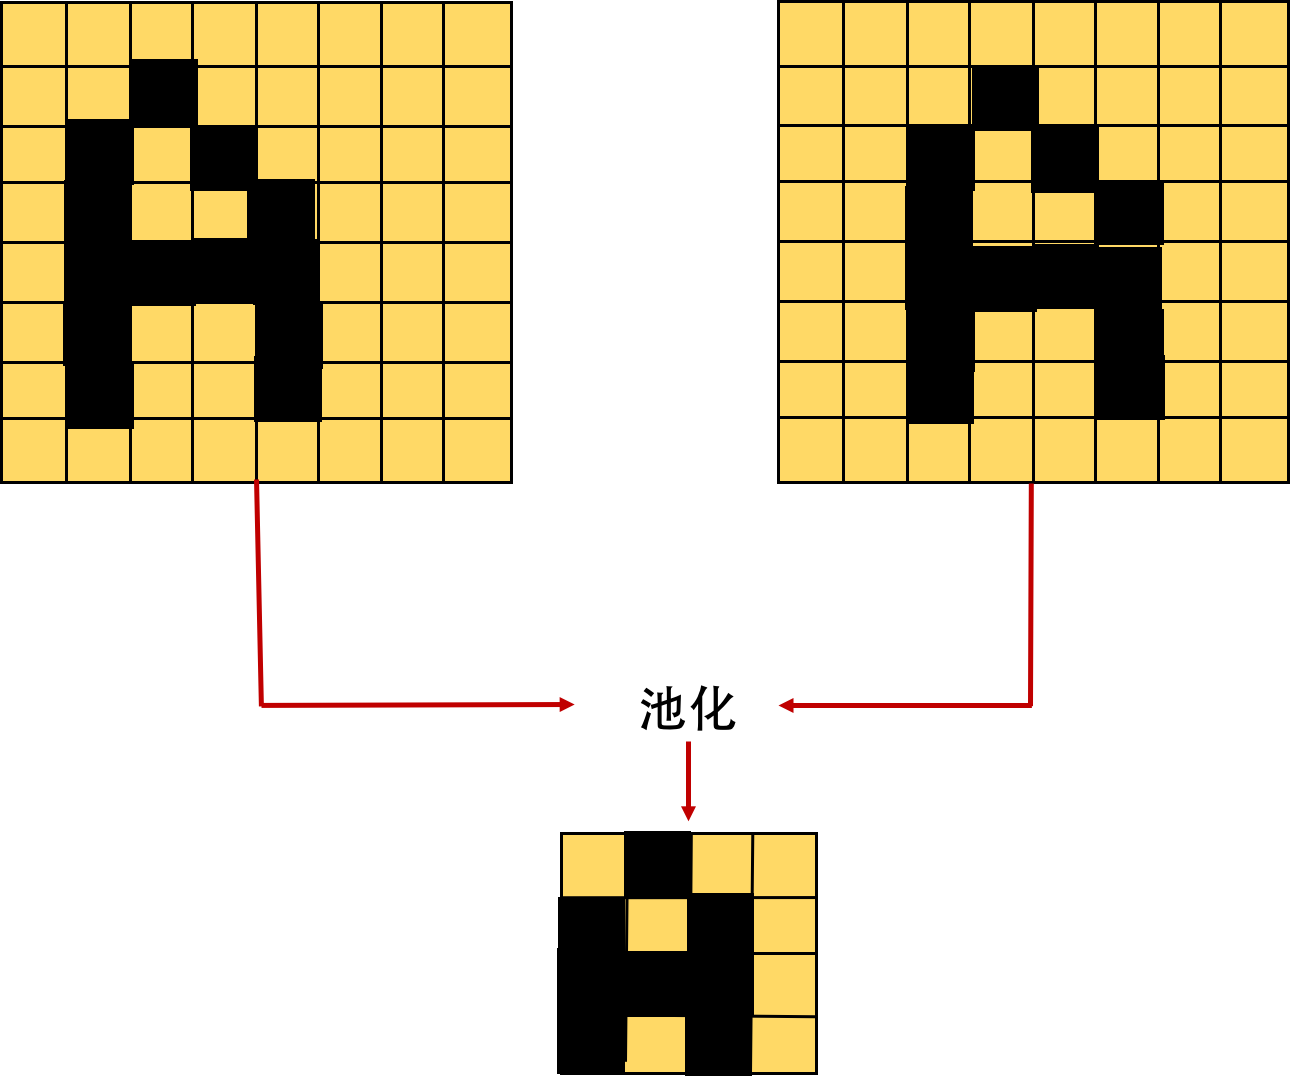
\includegraphics[width=1\linewidth]{intro_pooling.png}
\caption{池化操作的平移不变性。右图中的字母A相对于左图的A具有一个较为微小的平移,但是通过最大池化操作,却得到了完全相同的输出结果。即池化操作具有一定的特征不变性。}
\label{fig:intro_pooling}
\end{figure}

卷积神经网络中,卷积操作参数共享的性质使得卷积层具有了平移同变性。一个函数具有同变性是指,输出与输入具有相同的变化。对于图像卷积操作,通常会生成一个二维特征图,其中包含了输入图像中物体的位置信息。如果输入图像中的物体有所移动,经过相同的卷积操作,输出特征图中物体的特征也会进行同尺度的移动。平移同变性使得我们可以采用卷积操作提取图像的局部特征,例如图像处理过程中,提取图像的边缘特征是浅层网络的一个必要且有效的操作。而图像的边缘特征往往分布于整张图像的多处位置,因此在整张图像上采用权值共享是一个实际有效且十分可行的方案。但是在某些情况下,我们也许不希望采用参数共享,例如在人脸识别任务中,我们也许希望在人脸的不同位置提取不同的特征,例如在图像的上半部分提取眉毛特征,而在图像的下半部分查找出下巴等信息。卷积操作对平移具有同变性,但是对于缩放或旋转等变换并不具备同变性,需要卷积神经网络的其他机制去处理缩放和旋转问题。


池化操作是对相邻位置特征分布的统计输出,例如最大池化操作输出了相邻矩形区域内特征的最大值。池化可以使特征具有一定程度的平移不变性。也就是说如果我们将输入图像上的物体进行较小的平移,池化的输出结果与平移前相同,如图~\ref{fig:intro_pooling}所示。图~\ref{fig:intro_pooling}对于一个具有微小平移的两幅输入图像,同时进行最大池化进行特征提取,可以得到完全相同的输出结果。对于一些位置无关的图像识别任务,平移不变性是一个特征提取与分类的有效手段。池化的使用相当于我们给待处理的问题引入了平移不变性的先验知识,如果待处理的问题确实具有这样的性质,可以极大地提高网络的统计特性。

\begin{figure}
\centering
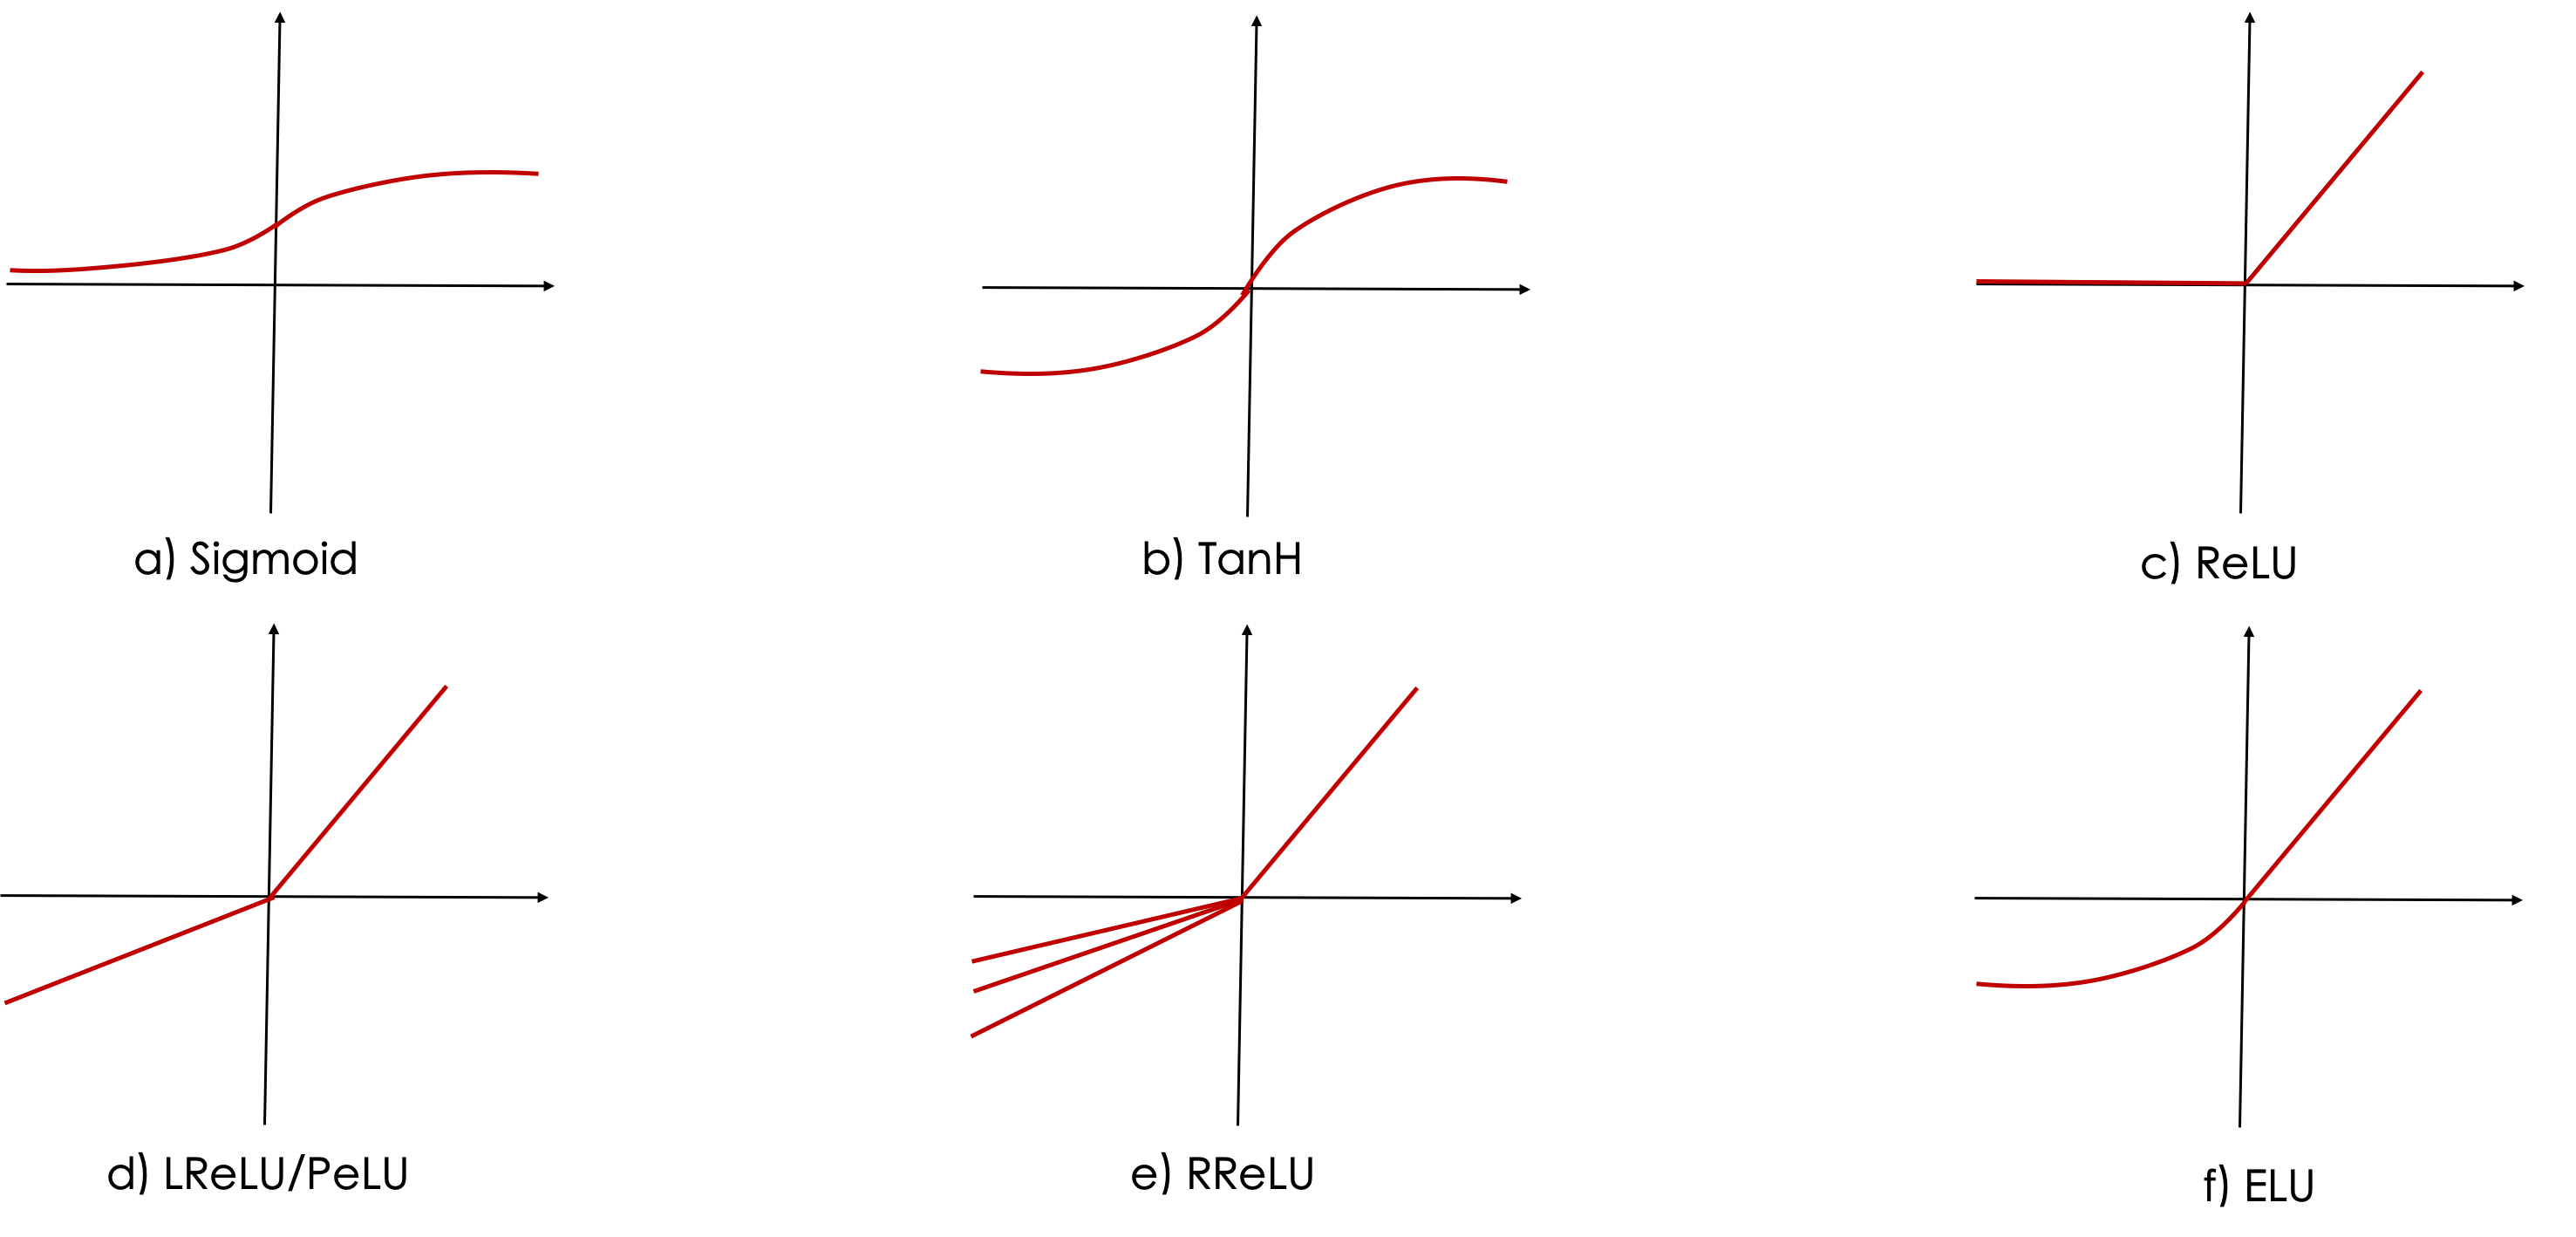
\includegraphics[width=1\linewidth]{intro_active.png}
\caption{不同激活函数的函数曲线对比图。}
\label{fig:intro_active}
\end{figure}

非线性激活函数可以增强卷积神经网络的非线性拟合能力,不同的激活函数形式,对网络的计算量、拟合和泛化能力具有重要的影响。ReLU~\cite{nair2010rectified}是目前卷积神经网络最常用的激活函数,它是一个作用于单像素的线性分段函数,ReLU保留正数输入不变同时将负的输入抑制为零,其函数形式可以表示为:
\begin{eqnarray} \label{equ:relu}
h_{i,j,k}=\max(x_{i,j,k},0)
\end{eqnarray}
其中$x_{i,j,k}$表示第 $k$ 个通道位置 $(i,j)$ 处的输入特征。相对于传统的Sigmoid函数:
\begin{eqnarray} \label{equ:sigmoid}
h_{i,j,k}=\frac{1}{1+e^{-x_{i,j,k}}}
\end{eqnarray}
和双曲正切函数:
\begin{eqnarray} \label{equ:tanh}
h_{i,j,k}=\frac{e^{x_{i,j,k}}-e^{-x_{i,j,k}}}{e^{x_{i,j,k}}+e^{-x_{i,j,k}}}
\end{eqnarray}
ReLU的计算更简单,并且在输出神经元中引入了稀疏的概念,可以得到稀疏的特征表示。但是对于未激活的神经元,ReLU的反向传播梯度为零,使得未激活的神经元无法进行参数更新。Mass等人~\cite{maas2013rectifier}提出斜坡线性整流单元(Leaky Rectified linear unit,LReLU)来解决这个问题,计算公式如下:
\begin{eqnarray} \label{equ:lrelu}
h_{i,j,k}=\max(x_{i,j,k},0)+{\lambda}\min(x_{i,j,k},0)
\end{eqnarray}
其中$\lambda$是一个预定义的取值在 $(0,1)$ 之间的随机变量。He等人~\cite{he2015delving}对LReLU进一步改进,提出了参数化线性整流单元(Parametric Rectified linear unit,PReLU),PReLU可以表示为:
\begin{eqnarray} \label{equ:prelu}
h_{i,j,k}=\max(x_{i,j,k},0)+{\lambda}_k\min(x_{i,j,k},0)
\end{eqnarray}
其中 ${\lambda}_k$ 是第 $k$ 个通道上的可学习参数。PReLU通过引入极少的参数,有效地提高了网络的拟合能力。对LReLU的另一项改进是Xu等人~\cite{xu2015empirical}提出的随机线性整流单元(Randomized Rectified linear unit,RReLU),与公式~\ref{equ:prelu}具有相同的形式,但是其中的 ${\lambda}_k$ 服从均匀分布,前向传播过程中通过随机采样产生。Clevert等人~\cite{clevert2015fast}提出了指数线性单元(Exponential Linear Unit,ELU),可以在加速网络的训练的同时,提高网络的识别率,ELU可以表示为:
\begin{eqnarray} \label{equ:elu}
h_{i,j,k}=\max(x_{i,j,k},0)+\min({\lambda}(e^{z_{i,j,k}}-1),0)
\end{eqnarray}
其中 $\lambda$ 是一个预定义的加权因子。上述六种非线性激活函数的关系与对比如图~\ref{fig:intro_active}所示。


\section{问题提出}
\label{sec:question}

卷积神经网络凭借局部感受野、权值共享、池化和分层特征提取四大特点,在计算机视觉领域特别是视觉物体识别任务上取得了重大的研究突破。自2012年Krizhevsky等人~\cite{krizhevsky2012imagenet}在ImageNet大规模视觉识别比赛夺冠之后,各种网络模型如ZFNet~\cite{zeiler2014visualizing},VGG~\cite{simonyan2014very},GoogLeNet~\cite{szegedy2014going,szegedy2015rethinking,szegedy2016inception}、ResNet~\cite{he2015deep}等被相继提出,用以解决物体分类问题。

但是对于一个新的物体识别问题,针对具体任务设计并实现一个有效网络模型仍然是一个困难的工作,网络深度的选择、感受野大小的选择和卷积核个数的选择都是网络在设计过程中普遍存在却又很难回答的问题。例如在深度选择上,VGG和GoogLeNet的成功说明了更深的网络结构可以提高网络的识别率,但是另一方面ResNet通过实验证实,随着网络的深度逐渐加深,网络的识别性能将趋于饱和甚至下降。尽管卷积神经网络具有卷积、池化和非线性化等通用的结构,但是整个网络的设计过程仍然是经验主义的。另一方面,在物体识别任务上,已经出现了很多结构功能各不相同的卷积神经网络模型,并且这些模型都在各自不同的领域得到了验证。对这些模型进行总结、归纳和积累,综合他们各自的优势,用于解决新的识别问题,这也是一个具有研究意义的课题。因此,本文提出了一种组合卷积结构,即自适应卷积模块,来简化复杂网络设计的过程。在组合卷积结构中,融合了四种模型的特点与优势,用以提高组合卷积结构的特征表达能力。

对于视觉物体识别任务,网络的泛化能力是一个重要的评价指标。卷积神经网络能够在物体识别任务上有效的一个关键因素就是大规模的标注数据,当我们无法获取更多的标注数据时,数据增广是一个直接有效的提高网络识别能力和泛化能力的方法。合理的数据增广方式,可以在保证不影响样本总体分布的前提下,扩展样本空间,增加输入图像的多样性。但是卷积神经网络采用分层的特征提取方式,并且特征在逐层提取的过程中会不断强化其旋转平移的不变性,因此从输入层到输出层,数据增广对网络的参数更新的影响会逐渐减弱。本文将数据增广的思想扩展到特征层,提出了随机区域池化方法,对池化层特征进行特征增广,在不改变特征空间样本分布的前提下,对特征进行扰动,增加特征的多样性。通过特征增广来增强网络的鲁棒性,提高网络的泛化能力。

卷积神经网络优越的识别能力往往来自于更深或更宽的网络结构和超大规模的计算。具有大量参数的卷积神经网络模型,在测试或预测阶段需要消耗大量的计算资源与时间,很难在实际生活中得到大规模的应用与推广。因为需要消耗大量的内存和计算资源,因此无法将应用部署于客户端;部署在高性能服务器,服务端也无法应对多用户的并发请求;就算只对单用户提供服务,用户端也无法接受长时间的请求等待。为了解决卷积神经网络应用的难题,早期的工作主要集中在硬件性能的提升,但硬件方面的研究进展已经无法满足人们对计算能力的需求,特别是在当今这样一个移动互联网时代,智能手机和平板电脑成为人们生活的主流产品,如何在一个低性能的CPU和只具有少量内存的GPU上运行深度卷积神经网络模型,逐渐引起学术界的关注。本文提出了一种新的基于矩阵低秩分解的卷积压缩方法主导卷积核分解,用于对卷积神经网络模型进行参数压缩与模型提速,并提出知识预回归的训练方法来尽力弥补由模型压缩所引起的精度损失。


\section{主要研究贡献}

针对上文提到的问题,本文针对物体识别问题,对卷积神经网络进行了研究与改进,主要研究贡献包括:

提出了一种组合卷积结构:自适应卷积模块,用于简化复杂卷积神经网络的设计过程,通过自适应卷积模块的简单堆叠,来自动实现复杂网络结构的设计。组合卷积结构结合了盗梦空间网络结构Inception、最大化输出单元Maxout、残差网络ResNet和网络中的网络NIN四个网络模型的优点,使得组合卷积结构具有更强的特征提取能力和更快的收敛速度。

提出了池化层的一种改进方法:随机区域池化,将数据增广的思想从数据层扩展到特征层,对卷积神经网络池化层的特征进行增广。随机区域池化通过随机放射变换对池化区域进行重采样,再对重采样之后的池化区域进行池化操作,因变换后的池化区域往往处于非整数边界,因此采用双线性差值对池化区域的像素进行估计。随机区域池化可以有效地增加特征的多样性,使网络对特征的扰动更加鲁棒,提高网络的泛化能力。

提出了一种基于主导卷积核分解和知识预回归的模型加速方法。主导卷积核分解是一种受矩阵低秩分解启发的卷积参数压缩方法,通过保留一个或多个具有主导作用的卷积核对卷积参数进行压缩。主导卷积核分解可以将卷积层的参数和计算量压缩到接近原来的12\%,极大地提高了模型的预测速度。为了弥补网络因压缩所造成的精度损失,受知识蒸馏方法启发,我们提出了知识预回归的网络训练方法,让压缩后的网络可以逐层地学习原网络的特征表达和泛化能力。

针对交通标志识别任务,我们将组合卷积结构和随机区域池化相结合,验证了两个方法的有效性。并采用基于主导卷积核分解和知识预回归的模型压缩方法对模型进行加速,最终得到一个具有较高识别率的快速交通标志识别模型。

\section{章节安排}


\begin{figure}[h]
\centering
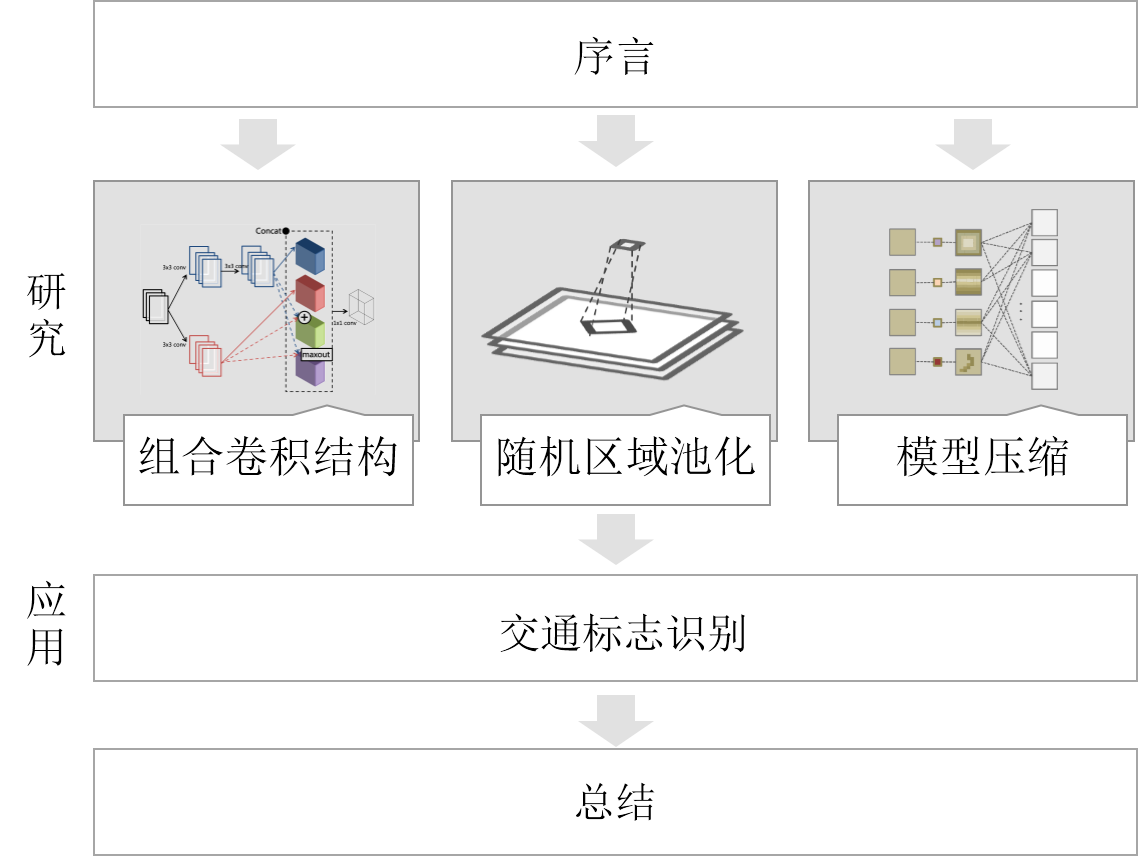
\includegraphics[width=0.8\linewidth]{intro_arc.png}
\caption{各章节关系图。}
\label{fig:intro_arc}
\end{figure}

本文共分为六章,各章之间的联系如图~\ref{fig:intro_arc}所示。各章的具体安排如下:

第一章为绪论,介绍了本文的研究背景与意义,调研了卷积神经网络近年来的发展现状,总结了在物体识别任务中卷积神经网络存在的问题,针对这些不足提出了本文的研究内容。

第二章为了简化复杂卷积卷积神经网络的设计过程,提出了一种组合卷积结构:自适应卷积模块,详细描述了组合卷积结构的实现细节,并以物体识别任务为例对其进行了实验验证与分析。

第三章为了提高网络的泛化能力,提出了池化层的一种改进方法随机区域池化,详细描述了随机区域池化的实现细节,并以物体识别任务为例验证了该方法的有效性。

第四章针对卷积神经网络的部署实施问题,提出了基于主导卷积核分解和知识预回归的模型压缩与加速方法,详细描述了卷积的压缩方法和网络的训练过程,并以物体识别任务为例对其进行了测试。

第五章针对一个实际问题:交通标志识别,对第二章的组合卷积结构和第三章的随机区域池化进行了对比与测试。并将两种方法结合,应用于交通标志识别任务。最后采用第四章的模型压缩方法对其进行加速,最终得到了一个具有较高识别精度的快速交通标志识别模型。

第六章是对全文工作的总结,并展望了未来可能的研究方向。


\chapter{组合卷积结构:自适应卷积模块}
\label{cha:sap}

\section{引言}
\label{sec:sap:introduction}
在过去的十几年时间里,卷积神经网络在计算机视觉领域取得了巨大的成功。尤其是在视觉物体分类、检测和分割等任务中,卷积神经网络的检测与识别精度远远超过了传统方法,连续打破了多项公开数据集的记录。通过卷积神经网络学习得到的特征,比传统人工设计的特征(例如SIFT~\cite{lowe1999object, ke2004pca,ke2004pca}特征和HOG~\cite{dalal2005histograms}特征等)更为有效,使得卷积神经网络在计算机视觉的多项任务中均取得了重大的研究突破。

视觉物体识别是计算机视觉领域一个经典的问题。很多有效的卷积神经网络模型,例如盗梦空间网络结构Inception~\cite{szegedy2014going,szegedy2015rethinking,szegedy2016inception},最大化输出单元Maxout~\cite{goodfellow2013maxout},残差网络ResNet~\cite{he2015deep},和网络中的网络NIN(Network in Network)~\cite{DBLP:journals/corr/LinCY13}被学者们提出用来提升网络的识别能力。但是,对于一个新的问题,设计并实现一个有效网络模型仍然是一个困难的工作。例如,网络深度的选择就是一个很常见,却又很难回答的问题。VGG~\cite{simonyan2014very} 和GoogLeNet~\cite{szegedy2014going}提出,更深的网络可以提高网络的识别性能。但是,仍然有一些实验~\cite{he2015deep} 表明,在深度持续加深的过程中,网络的测试误差将会趋于饱和甚至下降。另一个需要面对的难题是感受野大小的选择问题,VGG~\cite{simonyan2014very}的成功说明采用 $3\times3$ 的感受野是一个有效的策略,更大的感受野可以通过多个 $3\times3$ 感受野大小的卷积堆叠来实现。

本章提出了一种组合卷积结构:自适应模块(Self-Adaptive Module,SAM),来简化复杂网络的设计过程。结合多个已被验证有效的卷积神经网络模型的优势,SAM被设计成一个通用的卷积模块,使用组合卷积结构可以简化深层卷积神经网络的设计过程。为了实现这样的目标,SAM必须具有自适应的能力。换句话说,SAM采用端到端学习的方式,根据具体需要,学习成最为合适的结构。这样,一个大规模的深度卷积神经网络就可以通过SAM层的简单堆叠来设计实现。本章提出的SAM结构以盗梦空间网络结构Inception~\cite{szegedy2014going,szegedy2015rethinking,szegedy2016inception}为基础框架,包括四条特征提取分支和一个选择器。四条分支中包含两条卷积分支,它们具有不同的深度和感受野;一条最大化输出单元Maxout\cite{goodfellow2013maxout}分支,用于增强SAM的非线性拟合与逼近能力;一条残差~\cite{he2015deep}分支,可以加快SAM的收敛速度。选择器~\cite{DBLP:journals/corr/LinCY13}通过监督学习的方式对特征进行选择,同时在一定程度上起到特征压缩,降低网络计算复杂度的目的。

我们在多个物体识别的数据库上对SAM进行了测试,在CIFAR-10~\cite{krizhevsky2009learning},CIFAR-100~\cite{krizhevsky2009learning},MNIST~\cite{lecun1998gradient}和SVHN~\cite{netzer2011reading}四个数据集上均取得了优越的性能。本章剩余内容组织如下:第~\ref{sec:sap:ralate}节简要综述了相关工作;第~\ref{sec:sap:review}节回顾了SAM直接继承的四个显著网络结构;第~\ref{sec:sap:model}节详细阐述了SAM的结构与特点;第~\ref{sec:sap:experiment}节对SAM进行了实验验证与对比分析;第~\ref{sec:sap:conclusion}节总结了本章的主要内容。


\section{相关工作}
\label{sec:sap:ralate}

据我们所知,最早的卷积神经网络模型是1975年Fukushima~\cite{fukushima1982neocognitron} 提出的认知机(Cognitron)~\cite{fukushima1975cognitron} 和神经认知机(Neocognitron)~\cite{fukushima1980neocognitron}模型。在他的重要论文~\cite{fukushima1982neocognitron} 中,提出了包含卷积、感受野~\cite{hubel1959receptive, hubel1962receptive}和池化等概念的神经认知机计算模型。1989年,LeCun~\cite{le1988theoretical, lecun1989backpropagation, le1990handwritten}将误差的反向传播(back-propagation)引入神经认知机模型,并且成功应用于手写体数字识别数据库MNIST上,奠定了现代卷积神经网络的计算框架。

2012年,Krizhevsky等人~\cite{krizhevsky2012imagenet}采用卷积神经网络,借助于高性能的GPU并行计算能力,在2012年ImageNet大规模视觉识别比赛(ImageNet Large Scale Visual Recognition Competition,ILSVRC)中夺冠,掀起了一波卷积神经网络在计算机视觉领域的热潮。此后,越来越多的深度卷积神经网络模型被应用于图像识别,例如OverFeat~\cite{sermanet2013overfeat},VGG~\cite{simonyan2014very},GoogLeNet~\cite{szegedy2014going,szegedy2015rethinking,szegedy2016inception} 和ResNet~\cite{he2015deep}.

在CIFAR-10~\cite{krizhevsky2009learning},CIFAR-100~\cite{krizhevsky2009learning},MNIST~\cite{lecun1998gradient}和SVHN~\cite{netzer2011reading} 四个个数据集上,Goodfellow等人~\cite{goodfellow2013maxout}提出了一种新的激活函数形式Maxout。Maxout具有很强的拟合能力,如果隐层具有足够多的神经元,理论上Maxout可以逼近任意函数。Lin等人~\cite{DBLP:journals/corr/LinCY13}采用网络中的网络模型(Network in Network,NIN)来提高模型局部感受野范围内的辨识能力,同时,Lin提出了全局池化来提取固定长度的特征用于分类,在一定程度上起到防止过拟合的效果。Wan等人~\cite{wan2013regularization}提出了DropConnect方法,该方法是对Dropout方法的推广,对全连接层进行正则化。Zeiler and Fergus~\cite{zeiler2013stochastic}对池化进行了改进,提出了随机池化,在池化区域根据多项式分布进行随机采样。Stollenga等人~\cite{stollenga2014deep} 将注意力模型引入卷积神经网络的卷积核,提出了dasNet。Lee等人~\cite{lee2014deeply}通过同时对网络的隐层和输出层进行监督学习,提出了深度监督网络(Deeply-Supervised Nets,DSN)。Liang和Hu~\cite{liang2015recurrent}通过在卷积层引入递归连接整合特征上下文信息,提出了递归卷积神经网络。Srivastava等人~\cite{srivastava2015training}通过允许特征以信息的形式通过高速通道跨层流动,提出了Highway网络,可以有效的提高网络的收敛速度。He等人\cite{he2015deep}提出了残差模型,设计并实现了ResNet网络,在CIFAR-10,ILSVRC 2015~\cite{everingham2010pascal}和COCO~\cite{lin2014microsoft}数据集上取得了巨大成功。

\section{显著模型的简要回顾}
\label{sec:sap:review}

本节简要回顾了四种用于视觉物体识别的卷积网络模型。SAM继承了这四个模型的优势,降低了复杂卷积网络的设计难度。

\begin{figure*}[t]
\centering
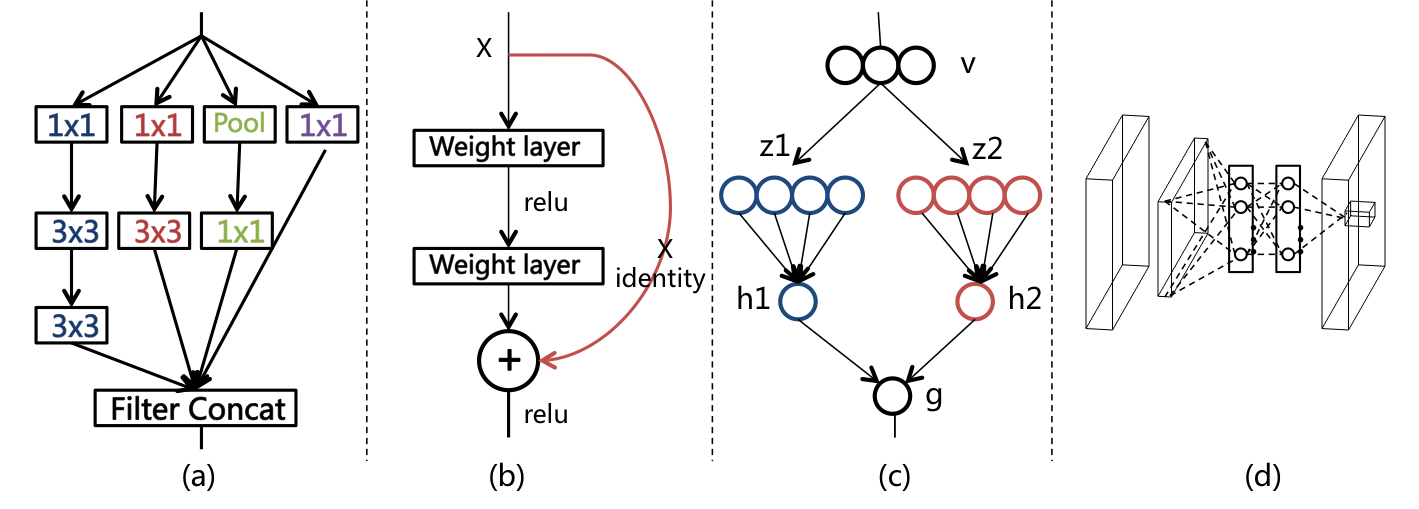
\includegraphics[width=1.0\linewidth]{sam_review.png}
\caption{显著模型的简要回顾. (a) Inception, (b) ResNet, (c) Maxout, (d) NIN}
\label{fig:sam_review}
\end{figure*}

\subsection{Inception}
\label{sec:sap:review:inception}

盗梦空间网络结构Inception~\cite{szegedy2014going,szegedy2015rethinking,szegedy2016inception}出自GoogLeNet,用于调整网络计算资源的分配,提高计算资源的利用率。Inception通过精心的设计,使得网络深度和宽度增加的同时,计算负担基本保持不变。 Inception的结构如图~\ref{fig:sam_review}(a)所示,该结构的公式化描述如下:
\begin{eqnarray} \label{equ:inception}
f^{1} &=& \sigma(W_{13}\sigma(W_{12}\sigma(W_{11}x+b_{11})+b_{12})+b_{13})\nonumber\\
f^{2} &=& \sigma(W_{22}\sigma(W_{21}x+b_{21})+b_{22})\nonumber\\
f^{3} &=& \sigma(W_{31}pool(x)+b_{31})\nonumber\\
f^{4} &=& \sigma(W_{41}x+b_{41})\nonumber\\
f_{inception} &=& (f^1; f^2; f^3; f^4)
\end{eqnarray}
其中 $x$ 表示Inception模块的输入;采用线性整流单元 (Rectifier Linear Unit,ReLU) $\sigma$ 作为非线性激活函数;Inception模块的输出 $f_{inception}$ 是四条特征提取分支的并联。

\subsection{Maxout}
\label{sec:sap:review:maxout}

Maxout~\cite{goodfellow2013maxout}是Goodfellow等人提出的新型激活函数,通过对多各卷积通道求最大值的方式来提升网络的拟合能力。该方法常与Dropout配合使用,提高Dropout的多模型组合平均性能。Maxout可以有效地提高模型的非线性拟合与逼近能力,如图~\ref{fig:sam_review}(c)所示,单个Maxout单元可以公式化表示如下:
\begin{equation} \label{equ:maxout}
f_{maxout}(x)=\max\limits_{i\in[1,k]}(W_{i}x+b)
\end{equation}
其中 $x$ 表示Maxout单元的输入;对于Maxout单元结构,其输出 $f_{Maxout}$ 是 $k$ 个卷积层对应位置的最大值。在~\cite{goodfellow2013maxout}论文中还论证了,具有两个隐层的Maxout网络理论上可以以任意精度逼近任何连续函数。


\subsection{ResNet}
\label{sec:sap:review:resnet}

残差网络(Residual Network,ResNet)~\cite{he2015deep}是一个更容易优化与收敛的残差学习框架,ResNet有助于减轻网络的训练负担。ResNet将隐层的输出结果当做与输入相关的残差学习函数,而不是去直接学习相对于输入的复杂函数,如图~\ref{fig:sam_review}(b)所示,ResNet可以公式化表示如下:
\begin{equation} \label{equ:resnet}
f_{resnet}(x)=\mathcal{F}(x, W_i) + W_{s}x
\end{equation}
其中 $x$ 表示ResNet的输入;线性映射 $W_s$ 用于匹配特征维度;函数 $\mathcal{F}(x, W_i)$ 表示需要学习的残差函数,在图~\ref{fig:sam_review}(b)中,$\mathcal{F} = W_{2}\sigma(W_{1}x+b, 0)$;同样采用线性整流单元 $\sigma$ 作为非线性激活函数。ResNet更加容易收敛与优化,并且可以通过持续增加网络深度来获取更高的网络泛化能力。

\subsection{NIN}
\label{sec:sap:review:nin}

网络中的网络(Network in Network,NIN)~\cite{DBLP:journals/corr/LinCY13}用于提升局部感受野范围内模型的辨识能力。传统的卷积层采用线性卷积核和非线性激活函数来产生输出。NIN在卷积层嵌入一个小型网络,采用更加复杂的非线性激活函数在感受野范围内对输入数据进行抽象。如图~\ref{fig:sam_review}(d),NIN可以公式化表示为:
\begin{eqnarray} \label{equ:nin}
f_{k_1}^{1}&=&\sigma(W_{k_1}^{1}x+b_{k_1}) \nonumber\\
f_{k_2}^{2}&=&\sigma(W_{k_2}^{2}f^{1}+b_{k_2}) \nonumber\\
\cdots&\nonumber\\
f_{k_n}^{n}&=&\sigma(W_{k_n}^{n}f^{n-1}+b_{k_n})
\end{eqnarray}
其中 $n$ 表示NIN非线性网络的层数;同样采用线性整流单元 $\sigma$ 作为非线性激活函数。从另一个角度观察,NIN等价于在传统卷积层嵌入了一个或多个 $1\times1$ 感受野大小的卷积层,这种解释对NIN结构的理解更为直观。

\section{组合卷积结构}
\label{sec:sap:model}

第~\ref{sec:sap:review}节简要介绍了四个卷积网络模型的结构特点与优势,本节通过结合上述四个网络模型各自的优势,提出了一种组合卷积结构:自适应卷积模块(Self-Adaptive Module,SAM)。在本节最后,讨论了组合卷积结构的特点。

\subsection{SAM结构}
\label{sec:sap:model:arc}

\begin{figure}[h]
\centering
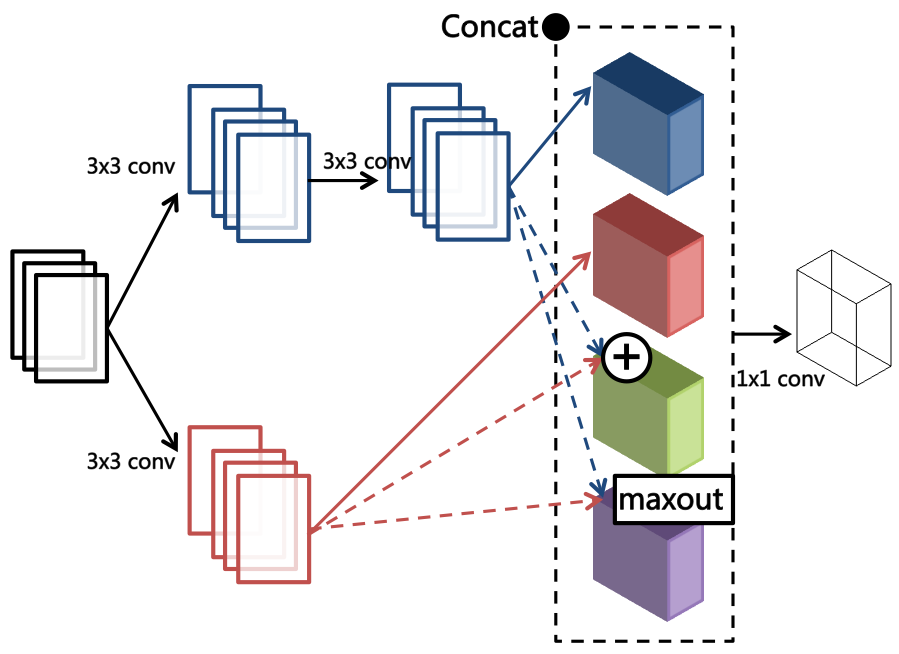
\includegraphics[width=1.0\linewidth]{sam_arc.png}
\caption{SAM结构。}
\label{fig:sam}
\end{figure}

结合盗梦空间网络结构Inception,最大化输出单元Maxout,残差网络ResNet,网络中的网络NIN这四个网络模型各自的优势,本节设计并实现了一种组合卷积结构:自适应模块SAM。SAM以盗梦空间网络结构Inception为计算框架,包括四条特征分支和一个选择器。如图~\ref{fig:sam}所示,四条分支中包括两条具有不同深度和感受野的卷积分支,一条Maxout分支,一条残差分支。SAM可以公式化表示如下:
\begin{eqnarray} \label{equ:sam}
f^{1} &=& W_{11}x+b_{11} \nonumber\\
f^{2} &=& W_{22}\sigma(BN(W_{21}x+b_{21}))+b_{22} \nonumber\\
f^{3} &=& f^{1}+f^{2} \nonumber\\
f^{4} &=& \max(f^1, f^2) \nonumber\\
f^{c} &=& {\sigma}(BN(f^1; f^2; f^3; f^4)) \nonumber\\
f_{SAM} &=& {\sigma}(BN(W_{s}f^{c}+b_{s}))
\end{eqnarray}
其中 $f^{1}$ 是第一条卷积分支,具有 $3\times3$ 的感受野和 1 的深度;$f^{2}$为第二条卷积分支,通过具有 $3\times3$ 感受野大小的两个卷积层的堆叠,$f^{2}$ 具有 $5\times5$ 的感受野和 2 的深度;$BN$ 代表批正则化(Batch Normalization,BN)~\cite{ioffe2015batch}操作;$f^{3}$ 是 $f^{1}$ 和 $f^{2}$ 的和,该分支是残差分支,通过线性映射矩阵 $W_{11}$ 将输入 $x$ 映射为 $f^{1}$ , $f^{1}$ 与 $f^{2}$ 具有相同的维度,将 $f^{1}$ 加到 $f_{2}$ 上,使 $f_{2}$ 去学习相对于输入 $x$ 的残差函数,该分支的存在可以有效地加快SAM网络的训练过程,使网络更容易收敛;$f^{4}$ 是 $f^{1}$ 和 $f^{2}$ 的Maxout输出,用于增强SAM结构的非线性拟合能力,提高SAM网络的识别能力;$f^{c}$ 是四条分支的并联;最有通过一个具有 $1\times1$ 感受野大小的卷积层对 $f^{c}$ 特征进行筛选与组合。此外,选择器还可以增强SAM结构在局部感受野范围内的特征拟合能力,在一定程度上还起到特征压缩,降低后续网络计算复杂度的效果。

\subsection{SAM的分析与讨论}
\label{sec:sap:model:discuss}

SAM的设计以盗梦空间网络结构Inception为基础框架,这使得SAM可以更为自由的平衡特征的提取能力和网络的计算负荷。事实上,Inception也具有四条分支,分别是具有$1\times1$,$3\times3$ 和 $5\times5$ 的三个卷积层,和一个池化分支。换一个方式理解,Inception的优势是可以帮助我们在不同感受野的卷积和池化操作中作出一个最优的组合。我们将这样的思想扩展到四个更加复杂、计算量更小、拟合能力更强、更容易收敛的另外4个分支中。SAM具有两条卷积分支,分别具有 $3\times3$ 和 $5\times5$ 的感受野,一条残差分支,和一条Maxout分支。SAM的选择器用于合并这四条分支的特征,同时进行特征压缩与选择。SAM去掉了原Inception结构中 $1\times1$ 的卷积分支和池化分支,在我们的实验中,这两条分支对精度的影响不大,但引入这两条分支会增加网络额外的计算负荷。

ResNet可以加快深层网络的收敛速度,通过增加一条或多条从浅层到深层的跨层特征连接,来构建残差学习框架。He等人~\cite{he2015deep}的研究结果表明,当网络层数增加时,网络的测试精度会趋于饱和甚至下降。残差模型可以有效地克服这个问题,通过增加网络的深度来提高网络的泛化能力。SAM通过引入一条残差分支来继承残差模型的优势。值得一提的是,SAM通过复用 $f^{1}$ 和 $f^{2}$ 分支的计算结果来降低参数规模与计算量。SAM复用 $W_{11}$ 作为输入数据的线性投影矩阵,复用 $W_{21}$ 和 $W_{21}$ 作为残差模型中主分支的卷积参数矩阵,如图~\ref{fig:sam_review}(b)所示。

Maxout常常与Dropout一起被当做是一种模型平均技术来使用,理论上Maxout可以逼近任意连续函数。但是Maxout的计算负担较重,需要较大的参数数量和计算量。SAM引入了Maxout作为四条分支之一,为了克服Maxout计算负担重的缺陷,我们同样复用了 $f^{1}$ 和 $f^{2}$ 分支来降低模型的参数和计算复杂度。该分支的引入可以有效地提高SAM结构的拟合能力。

NIN主要用于提高局部感受野范围内的模型辨识能力,事实上,NIN等价于在输出特征后面增加一或多个具有 $1{\times}1$ 感受野大小的卷积层。这样的结构在SAM中起到十分关键的作用。首先,该结构可以压缩特征的维度,从而减小运行时内存消耗与计算负担。其次,该结构起到特征选择的作用,通过监督学习的方式,合理分配各特征的权重。最后,该结构增加了特征的非线性拟合能力,可以有效地提升SAM的局部辨识能力。

实际上,SAM并不局限于只有这四条分支,更多的优秀的模型分支有待加入SAM结构,对SAM进行改进与性能提升。

\section{实验结果}
\label{sec:sap:experiment}

在深度学习开源项目caffe~\cite{jia2014caffe}的基础上,我们实现并测试了组合卷积结构SAM。所有的实验均以数据并行的方式运行于具有2颗GPU核心的NVIDIA K80上。我们在四个图像识别数据集上对SAM进行了测试,其中包括CIFAR-10~\cite{krizhevsky2009learning},CIFAR-100~\cite{krizhevsky2009learning},MNIST~\cite{lecun1998gradient}和SVHN~\cite{netzer2011reading}。

\subsection{网络结构}
\label{sec:sap:experiment:arc}

\begin{figure}[t]
\centering
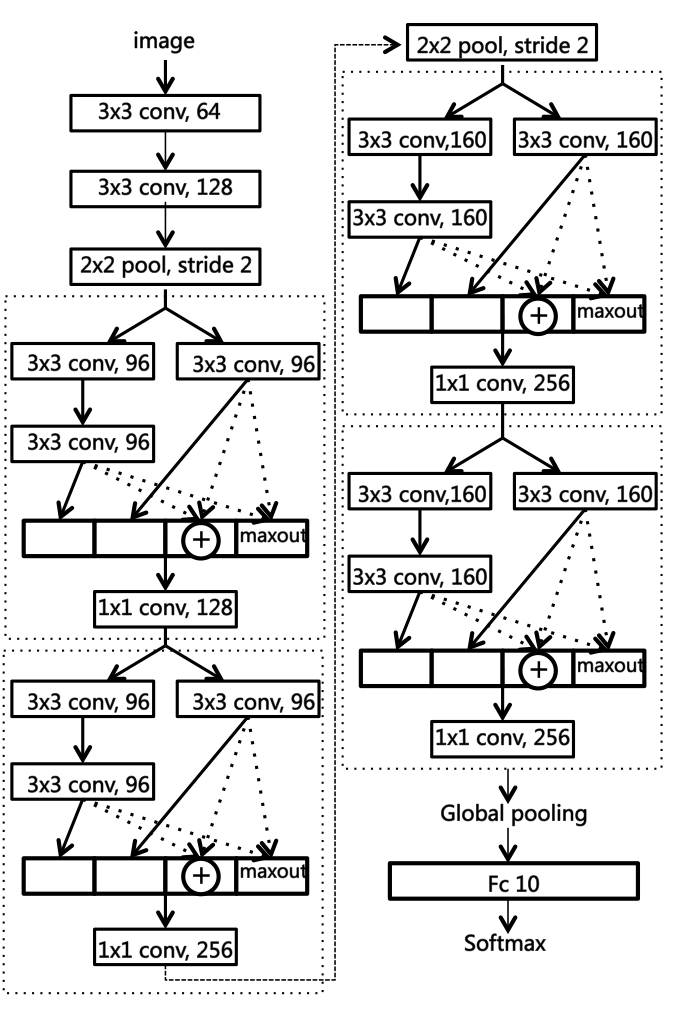
\includegraphics[width=0.8\linewidth]{sam_net.png}
\caption{SAM-Net:网络整体结构。}
\label{fig:net}
\end{figure}

本节所使用的网络结构如图~\ref{fig:net}所示,该网络包含了两个卷积层,四个SAM层,三个均值池化层和一个softmax层。

通常来说,卷积神经网络的初始阶段主要用于提取图像的简单特征,传统的卷积层在网络的初始阶段已经表现的足够优秀,并且可以节省大量的计算开销。因此,SAMNet的初始阶段是两个传统卷积层,一个均值池化层紧随其后。接下来,SAMNet采用两个SAM卷积层组成了网络的中间阶段,再经过一次均值池化,另外两个SAM层组成了SAMNet的下一个阶段。输入图像经过以上两个卷积层和四个SAM层所生成的特征连接到了一个全局均值池化层,最后通过Softmax层预测各类别的概率分布。此外,批规划化BN作用于每个卷积层之后,对特征进行正则化。

\subsection{网络参数}
\label{sec:sap:experiment:param}

\begin{figure}[!h]
\centering
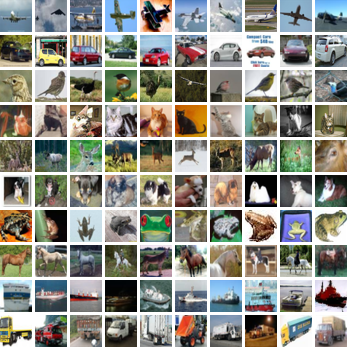
\includegraphics[width=1\linewidth]{sam_cifar10.png}
\caption{CIFAR-10测试样本示例。图中一共 10 行,每一行代表一个类别,从上到下分别是飞机、汽车、鸟、猫、鹿、狗、青蛙、马、轮船、卡车。每个类别分别列举了 10 张训练图像,因为原始图片的大小仅仅具有 $32\times32$ 像素大小,显示略显模糊。}
\label{fig:sam_cifar10}
\end{figure}


在所有的实验中,我们均采用批大小为96的随机梯度下降(Stochastic Gradient Descent,SGD)算法来训练SAMNet。网络的初始学习率为 0.01,在训练过程中,每当损失函数达到局部极值而停止下降时,学习率被降低为原来的 $1/10$。持续减小学习率三次,直到学习率降低至 1e-5。在卷积层,卷积偏置的学习率是卷积核的 2 倍。训练过程中,采用 0.9 的动量因子(Momentum)来保证随机梯度下降算法的快速稳定。所有的参数均采用 0.004 的权重衰减(Weight Decay )。丢弃率为 0.1 的Dropout被用于除了第一层卷积之外的每个卷积层之前。对于四个数据集,我们均采用了相同的数据预处理,在训练数据集上计算出所有图像对应位置的BGR像素均值,记为像素均值图像,网络的输入图像是原始图像与像素均值图像的差。

\subsection{CIFAR-10}
\label{sec:sap:experiment:cifar10}

首先从CIFAR-10~\cite{krizhevsky2009learning}开始我们实验,Cifar是加拿大政府牵头投资的一个科研项目研究所,CIFAR-10是Hinton的两个学生Alex Krizhevsky和Ilya Sutskever整理收集的一个物体识别数据集。CIFAR-10的图像是八千万微图片(80 Million Tiny Images Dataset)的一个标注子集,一共包含 60,000 张 $32\times32$ 的彩色图片,平均分为完全互斥的 10 类,每类具有 6,000 张图片。整个数据集被分成 5 组训练样本和 1 组测试样本,每组具有 10,000 张图片,即一共有 50,000 张训练图片和 10,000 张测试图片。CIFAR-10一共包含10个类别,分别是飞机、汽车、鸟、猫、鹿、狗、青蛙、马、轮船、卡车,如图~\ref{fig:sam_cifar10}。图~\ref{fig:sam_cifar10}一共十行,每行代表一个类别,每类列举了十张训练样本,因为原始图片仅仅具有 $32\times32$ 像素大小,因此显示略显模糊。

\begin{table}[h]
\caption{CIFAR-10数据集上与已知模型的对比试验。}
\label{tab:cifar10}
\centering
 \begin{minipage}[t]{0.8\textwidth} 
 \begin{tabularx}{\linewidth}{L{6cm}C{4cm}}
 \toprule[1.5pt]
%\begin{tabular}{L{6cm}C{4cm}}
{\heiti 模型} & {\heiti 测试错误率(\%)} \\
\midrule[1pt]
\multicolumn{2}{c}{\heiti 没有数据增广} \\
\hline
Maxout \cite{goodfellow2013maxout}  & 11.68 \\
Prob maxout~\cite{springenberg2013improving}  & 11.35 \\
NIN~\cite{DBLP:journals/corr/LinCY13}  & 10.41 \\
DSN~\cite{lee2014deeply} &9.69 \\
%RCNN-96~\cite{liang2015recurrent} & 0.67 M & 9.31 \\
%RCNN-128~\cite{liang2015recurrent} & 1.19 M & 8.98 \\
RCNN~\cite{liang2015recurrent} & \bf{8.69} \\
ALL-CNN~\cite{springenberg2014striving} & 9.08 \\
\hline
SAMNet & \bf{7.53 (7.53${\pm}$0.17)} \\
\midrule[1pt]
\multicolumn{2}{c}{\heiti 有数据增广} \\
\hline
Maxout~\cite{goodfellow2013maxout} & 9.38 \\
Prob maxout~\cite{springenberg2013improving} & 9.39 \\
dasNet~\cite{stollenga2014deep} & 9.22 \\
DropConnect~\cite{wan2013regularization} & 9.32 \\
NIN~\cite{DBLP:journals/corr/LinCY13} & 8.81 \\
DSN~\cite{lee2014deeply} & 7.97 \\
%RCNN-96~\cite{liang2015recurrent} & 0.67 M & 7.37 \\
%RCNN-128~\cite{liang2015recurrent} & 1.19 M & 7.24 \\
RCNN~\cite{liang2015recurrent} & 7.09 \\
Highway Network~\cite{srivastava2015training} & 7.54(7.72$\pm$0.16) \\
ALL-CNN~\cite{springenberg2014striving}  & 7.25 \\
%ResNet-20~\cite{he2015deep} & 0.27 M & 8.75 \\
%ResNet-32~\cite{he2015deep} & 0.46 M & 7.51 \\
%ResNet-44~\cite{he2015deep} & 0.66 M & 7.17 \\
%ResNet-56~\cite{he2015deep} & 0.85 M & 6.97 \\
ResNet~\cite{he2015deep} & \bf{6.43 (6.61$\pm$0.16)} \\
%ResNet-1202~\cite{he2015deep} & 19.4M & 7.93 \\
\hline
SAMNet & \bf{5.76 (5.76$\pm$0.13)} \\
 \bottomrule[1.5pt]
%\end{tabular}
 \end{tabularx}
\end{minipage}
\end{table}


为了验证SAM结构的有效性,我们在没有进行数据増广的情况下对SAMNet进行了测试,并且将实验结果与已知模型进行对比分析,实现结果如表~\ref{tab:cifar10}所示。因为网络参数的初始化采用了高斯随机初始化,为了避免单次实验结果的偶然性,我们对SAMNet进行了六次实验测试,分别得到7.52\%,7.76\%,7.34\%,7.54\%,7.35\%和7.68\%的测试错误率,即SAMNet在CIFAR-10上取得了一个均值为7.53\%,标准差为0.17\%的测试错误率。由表~\ref{tab:cifar10}可以看出,SAM-Net以1.16\%的优势超过了递归卷积神经网络RCNN~\cite{liang2015recurrent}。

\begin{figure}[!h]
\centering
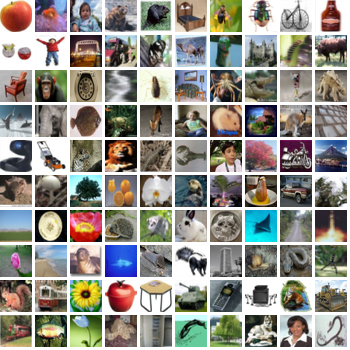
\includegraphics[width=1.0\linewidth]{sam_cifar100.png}
\caption{CIFAR-100测试样本示例。图中一共 100 张图像,每张图像展示了CIFAR-100数据集对应的一个类别。因为原始图片的大小仅仅具有$32\times32$ 像素大小,显示略显模糊。}
\label{fig:sam_cifar100}
\end{figure}


为了和之前的工作~\cite{goodfellow2013maxout,springenberg2013improving,stollenga2014deep,wan2013regularization,DBLP:journals/corr/LinCY13,lee2014deeply,liang2015recurrent,srivastava2015training,springenberg2014striving}保持一致,我们在有数据增广的情况下,对SAM-Net进行了实验测试。我们采用平移和图像水平翻转的数据增广方式,随机地从原始图像中截取 $24\times24$ 像素大小的图像样本,并随机的对其进行水平翻转。在测试阶段,对每张测试图片,从图像的四角和中心位置截取出五张 $24\times24$ 像素大小的图像,并对这五张测试图像进行水平翻转,得到一共十张图像进行测试。最终的测试结果是这十张图像预测概率的平均值。我们同样进行了六次实验,分别得到5.98\%,5.82\%,5.70\%,5.67\%,5.78\%和5.63\%的测试错误率,最终得到了均值为 5.76\%,标准差为0.13\%的测试误差率。SAMNet的性能甚至超过了最有 100 层结构之深的ResNet~\cite{he2015deep}网络,可见多个SAM卷积模块的简单组合,可以实现复杂网络结构的识别性能。



\subsection{CIFAR-100}
\label{sec:sap:experiment:cifar100}



CIFAR-100~\cite{krizhevsky2009learning}是一个与 CIFAR-10 类似的数据集,不同之处在于CIFAR-100具有 100 个物体类别。两个数据集具有相同的训练和测试图像规模,因此 CIFAR-100 中每个类别中图片数量只有CIFAR-10的 $1/10$。CIFAR-100的训练图像示例如图~\ref{fig:sam_cifar100} 所示,图~\ref{fig:sam_cifar100} 中包括 100 张图片,每张图片代表了 CIFAR-100 的一个物体类别,因为原始图像的分辨率较低,图像略显模糊。

\begin{table}[h]
\caption{CIFAR-100数据集上与已知模型的对比试验。}
\label{tab:cifar100}
\centering
\begin{tabular}{L{6cm}C{4cm}}
 \toprule[1.5pt]
{\heiti 模型} & {\heiti 测试错误率(\%)} \\
\midrule[1pt]
Maxout \cite{goodfellow2013maxout} & 38.57 \\
Prob maxout~\cite{springenberg2013improving}  & 38.14 \\
dasNet~\cite{stollenga2014deep}  & 33.78 \\
Tree based priors~\cite{srivastava2013discriminative} &  36.85 \\
NIN~\cite{DBLP:journals/corr/LinCY13} & 35.68 \\
DSN~\cite{lee2014deeply} & 34.57 \\
%RCNN-96~\cite{liang2015recurrent} & 0.67 M & 34.18 \\
%RCNN-128~\cite{liang2015recurrent} & 1.19 M & 32.59 \\
RCNN~\cite{liang2015recurrent} & \bf{31.75} \\
ALL-CNN~\cite{springenberg2014striving}  & 33.71 \\
\hline
SAMNet & \bf{28.56} \\
 \bottomrule[1.5pt]
\end{tabular}
\end{table}

在CIFAR-100数据集上,我们对本章提出的组合卷积网络进行了测试,采用与第~\ref{sec:sap:experiment:arc}节相同的卷积神经网络结构,与第~\ref{sec:sap:experiment:param}节相同的网络参数设置,SAMNet在CIFAR-100上取得了28.56\%的测试错误率。和其他网络结构相比,如表~\ref{tab:cifar100} 所示,SAMNet的识别性能比递归卷积神经网络RCNN~\cite{liang2015recurrent}提高了3.19\%,而在网络结构的设计上,采用组合卷积层搭建的SAMNet的设计更加简化与自由。


尽管CIFAR-100与CIFAR-10具有相同的训练数据总量,但是类别的增加(增加十倍),单类别中图像样本数量的减少(较少十倍),增加了物体识别的难度。对于卷积神经网络来说,训练样本的数量对网络的识别能力具有重要的影响。增加训练样本的数量,有助于提高卷积神经网络的泛化能力。对于每一个待识别的物体类别,卷积网络见过的图像越多,越能提高识别的准确度。从图~\ref{fig:sam_cifar10} 和图~\ref{fig:sam_cifar100} 可以看出,CIFAR-100和CIFAR-10具有十分相似的训练样本,但是CIFAR-100中单类别训练样本比CIFAR-10少了十倍(即一个数量级),导致CIFAR-100的测试错误率仅仅才达到28.56\%,与CIFAR-10数据集上7.53\%的测试错误率相比,高出了20多个百分点。


\subsection{MNIST}
\label{sec:sap:experiment:mnist}

\begin{figure}[!h]
\centering
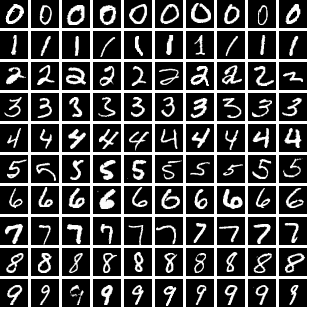
\includegraphics[width=1.0\linewidth]{sam_mnist.png}
\caption{MNIST测试样本示例。图中一共包含十行,每行代表了0-9的一个手写体数字类别,每行包含十个同类的图像样本。}
\label{fig:sam_mnist}
\end{figure}

MNIST~\cite{lecun1998gradient}是阿拉伯数字 0-9 的手写体数字识别数据集,该数据集具有 60,000 张训练图像,10,000 张测试图像。每个手写体数字都被归一化居中显示在一个$28\times28$的灰度图像上,如图~\ref{fig:sam_mnist}所示,图~\ref{fig:sam_mnist}中一共包括十行,从上到下每行代表 0-9 的一个手写体类别,每一行列举了十张训练图像。

\begin{table}[h]
\caption{MNIST数据集上与已知模型的对比试验。}
\label{tab:mnist}
\centering
\begin{tabular}{L{6cm}C{4cm}}
 \toprule[1.5pt]
{\heiti 模型} & {\heiti 测试错误率(\%)} \\
\midrule[1pt]
Maxout \cite{goodfellow2013maxout}  & 0.45 \\
NIN~\cite{DBLP:journals/corr/LinCY13}  & 0.47 \\
DSN~\cite{lee2014deeply} & 0.39 \\
%RCNN-32~\cite{liang2015recurrent} & 0.08 M & 0.42 \\
%RCNN-64~\cite{liang2015recurrent} & 0.30 M & 0.32 \\
RCNN~\cite{liang2015recurrent} & \bf{0.31} \\
\hline
SAM-Net & \bf{0.31} \\
 \bottomrule[1.5pt]
\end{tabular}
\end{table}


相比于CIFAR-10与CIFAR-100的复杂彩色图像,MNIST数据集中手写体数字识别相对简单很多。使用与第~\ref{sec:sap:experiment:arc}节相同的卷积神经网络结构,与第~\ref{sec:sap:experiment:param}节相同的网络参数设置,SAMNet在MNIST数据集上取得了0.31\%的测试错误率,与递归卷积神经网络RCNN~\cite{liang2015recurrent}持平,如表~\ref{tab:mnist} 所示。组合卷积结构SAM,结合多个有效网络模型的优势,通过模型内多个复杂结构的有效组合,形成了一个通用的卷积神经网络模块,使用该模块有效地简化了深层卷积神经网络模型的设计过程。尽管MNIST 与 CIFAR-10 和 CIFAR-100 具有不同的训练样本,但是使用组合卷积结构设计实现的卷积神经网络模型SAMNet,采用相同的网络结构,在不同的数据集上均取得了较好的识别性能。可见,组合卷积结构在多个数据集上具有较强的通用性,且有效地简化了模型的实际过程。

\subsection{SVHN}
\label{sec:sap:experiment:svhn}

\begin{figure}[!h]
\centering
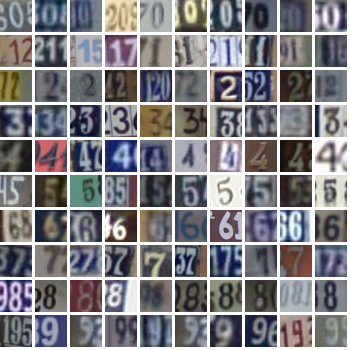
\includegraphics[width=1.0\linewidth]{sam_svhn.png}
\caption{SVHN测试样本示例。图中一共包含十行,从上到下每行代表了一类谷歌街景的房牌号码,每类房牌号列举了十张训练样本图像。}
\label{fig:sam_svhn}
\end{figure}

SVHN~\cite{netzer2011reading}是一个采集自真实环境的图像数据集,其中的图片采集自谷歌街景中的房牌号。SVHN提供了两种格式的数据,这里我们采用第二种格式。该数据集包含了 73,257 张训练图像,26,032 张测试图像,和额外的 531,131 张相对比较简单的附加训练图像。SVHN数据集比MNIST更加复杂,识别难度也更大。因为SVHN的图片采集自真实环境,图片的亮度与光照变化较大。并且SVHN的单张图像中可能会出现多个数字,这种情况,我们只识别中间位置的数字,如图~\ref{fig:sam_svhn}所示。图~\ref{fig:sam_svhn}中包括十行,从上到下每行代表一类样本,每类包含十张测试图像样本。

我们采用与Goodfellow~\cite{goodfellow2013maxout}相类似的训练和测试步骤。从训练数据的每个类别中选取 400 张图像,从附加的简单训练样本中每个类别选取 200 张图像,合在一起作为验证集,用于调节网络的学习率与迭代次数。在SVHN数据集上,SAMNet取得了1.98\%的测试错误率,实验结果略差于递归卷积神经网络RCNN~\cite{liang2015recurrent},如表~\ref{tab:svhn}所示。注意到递归卷积神经网络RCNN在四个数据集上采用相似的递归卷积结构,不同参数规模的网络对四个数据集进行的训练与测试。本章所提出的有组合卷积结构搭建的卷积神经网络模型,在四个数据集上采用的是完全相同的网络结构和参数配置,具有更强的模型通用性。此外,本章提出的组合结构,不仅适用于本章提出的SAMNet,也可用于构建其他更宽更深的卷积神经网络结构,通过组合卷积的简单堆叠,来实现更复杂卷积网络结果的设计与优化。

\begin{table}[!h]
\caption{SVHN数据集上与已知模型的对比试验。.}
\label{tab:svhn}
\centering
\begin{tabular}{L{6cm}C{4cm}}
 \toprule[1.5pt]
{\heiti 模型} & {\heiti 测试错误率(\%)} \\
\midrule[1pt]
Maxout \cite{goodfellow2013maxout} & 2.47 \\
Prob maxout~\cite{springenberg2013improving} & 2.39 \\
NIN~\cite{DBLP:journals/corr/LinCY13} & 2.35 \\
DSN~\cite{lee2014deeply}  & \bf{1.92} \\
RCNN~\cite{liang2015recurrent}  & \bf{1.77} \\
\hline
SAM-Net & \bf{1.98} \\
 \bottomrule[1.5pt]
\end{tabular}
\end{table}


\subsection{可视化}
\label{sec:sam:vis}

卷积神经网络在物体识别任务上取得了重大的研究突破,为了深入理解卷积神经网络的特征提取过程,本小结对卷积神经网络的浅层卷积核与各卷积层特征进行了可视化与分析。

\begin{figure*}[h]
\centering
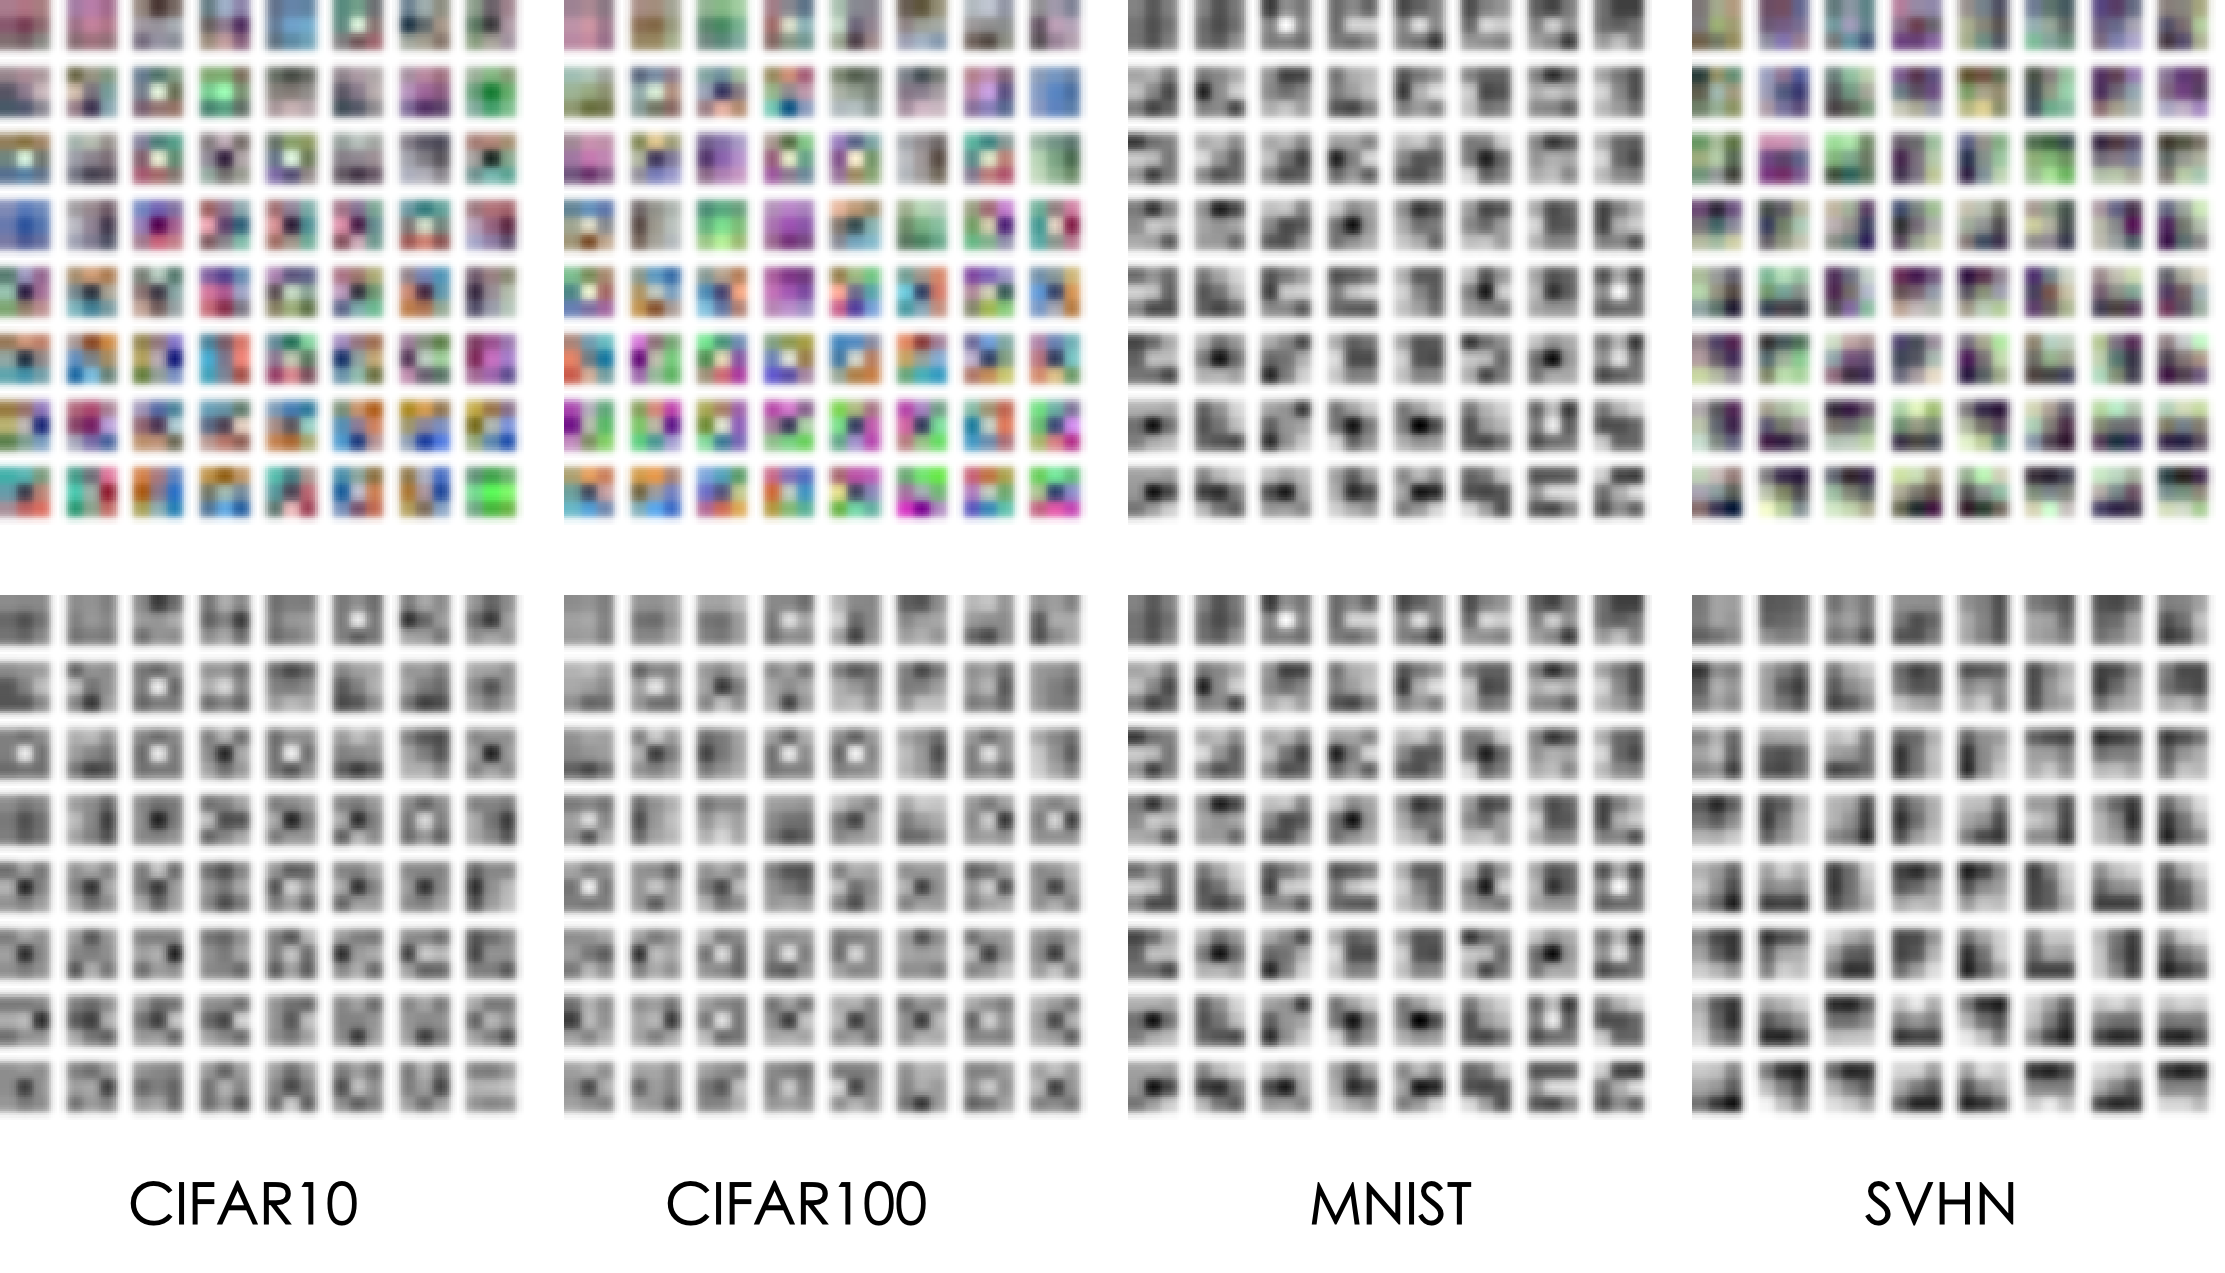
\includegraphics[width=1.0\linewidth]{sam_vis_filter.png}
\caption{第一层卷积核参数可视化。同一个神经网络模型SAMNet,在四个不同的数据集CIFAR-10、CIFAR-100、MNIST和SVHN上训练出的网络模型,第一个卷积层中64组卷积核参数可视化结果。将卷积核参数投影到图像像素空间,对于CIFAR-10、CIFAR-100和SVHN对应投影图像是三维彩色空间,对于MNIST因为输入只有单通道数据,投影后的卷积核可视化图像为灰度图。为了便于四个数据集卷积参数的对比,我们将所有图像转换为灰度图,如图中第二行所示,MNIST参数可视化结果保留不变。因卷积核大小仅仅为 $3\times3$,可视化图像大小也是 $3\times3$ 像素大小的图像,因此视觉效果较为模糊。}
\label{fig:sam_vis_filter}
\end{figure*}

我们首先对卷积神经网络的浅层卷积核进行了可视化,如图~\ref{fig:sam_vis_filter}所示。当网络训练完成之后,我们可视化了第一层卷积层中64组卷积核参数,将卷积核参数投影到图像空间。对于CIFAR-10、CIFAR-100和SVHN三个数据集,因为输入的图像为三通道彩色图像,因此对应的第一层卷积核也具有三个通道,可以将卷积核参数投影到图像BGR颜色空间。但是对于MNIST数据集,原始的输入图像是单通道灰度图,对应的第一层卷积核只具有一个通道,只能投影成灰度图。为了将四个数据集上学习到的卷积参数进行对比,我们将四个数据集上训练得到的特征核图像均转换成灰度图,对应的实验结果如图~\ref{fig:sam_vis_filter}第二行所示。

从图~\ref{fig:sam_vis_filter}中可以看出,四个数据集上学习出的第一层卷积核参数具有很高的相似度。这是因为对于卷积神经网络的浅层来讲,学习到的往往是一些颜色与边缘信息。此外,从图~\ref{fig:sam_vis_filter}可以看出,CIFAR-10与CIFAR-100的卷积核相似度最高,MNIST和SVHN的卷积核相似度较高。由此可见,对于相似的识别任务,学习到的卷积核也更为相似。

本章提出了组合卷积结构用于简化复杂的深层卷积神经网络的设计过程,融合了多个著名模型的主要优势,提出了自适应卷积模块SAM。SAM以Inception结构为基础计算框架,由四条特征提取分支与一个选择器组成,其中两条卷积分支具有不同的深度和感受野,一条残差分支用于加快SAM结构的收敛速度,一条Maxout分支用于提高SAM结构的非线性拟合能力。选择器具有特征压缩与组合的功能,增强局部感受野范围内的非线性拟合能力。为了更进一步地理解理解SAM的特征提取过程,我们对SAMNet各个卷积层特征进行了可视化分析。


\begin{figure}[h]
  \centering%
  \begin{subfigure}{0.13\textwidth}
    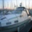
\includegraphics[width=1\linewidth]{sam_cifar10_in.png}
    \caption{输入图像。}
  \end{subfigure}%
  \hspace{1em}%
  \begin{subfigure}{0.8\textwidth}
    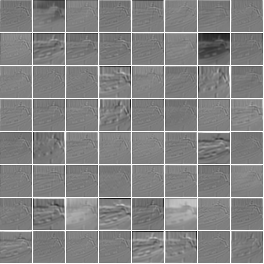
\includegraphics[width=1\linewidth]{sam_cifar10_conv1.png}
    \caption{第一个卷积层的输出特征图。}
  \end{subfigure}
  \caption{CIFAR-10数据集上,针对特定的输入图像,浅层卷积输出的特征图。浅层卷积可以提取图像的边缘角点等图像低层特征。}
  \label{fig:sam_cifar10_conv1}
\end{figure}


\begin{figure}[h]
  \centering%
  \begin{subfigure}{0.45\textwidth}
    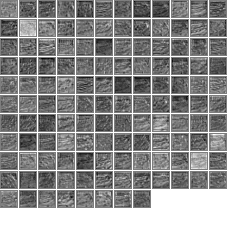
\includegraphics[width=1\linewidth]{sam_cifar10_conv2.png}
    \caption{第二个卷积层的输出特征图。}
  \end{subfigure}%
  \hspace{1em}%
  \begin{subfigure}{0.45\textwidth}
    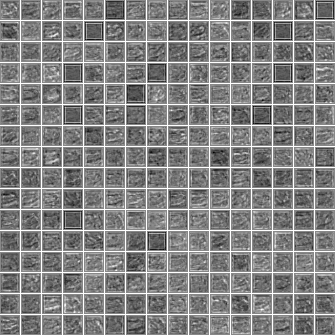
\includegraphics[width=1\linewidth]{sam_cifar10_conv3.png}
    \caption{第三个卷积层的输出特征图。}
  \end{subfigure}
  \caption{CIFAR-10数据集上,针对特定的输入图像,中层卷积输出的特征图。网络的中层特征图相对来说更为复杂,仍然可以辅助提取一些感受野更大的边缘与角点特征,但是更为主要的是网络已经开始提取图像的纹理等具有较高不变性的复杂特征。}
  \label{fig:sam_cifar10_conv3}
\end{figure}

\begin{figure}[h]
  \centering%
  \begin{subfigure}{0.45\textwidth}
    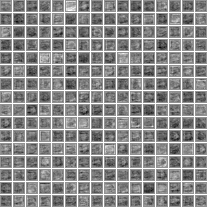
\includegraphics[width=1\linewidth]{sam_cifar10_conv4.png}
    \caption{第四个卷积层的输出特征图。}
  \end{subfigure}%
  \hspace{1em}%
  \begin{subfigure}{0.45\textwidth}
    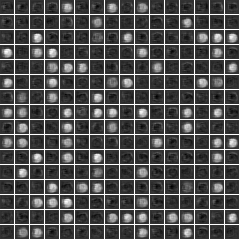
\includegraphics[width=1\linewidth]{sam_cifar10_conv5.png}
    \caption{第五个卷积层的输出特征图。}
  \end{subfigure}
  \caption{CIFAR-10数据集上,针对特定的输入图像,深层卷积输出的特征图。网络的高层提取的特征与物体的类别更加相关,且具有更强的不变性。往往可以提取出类别相关的物体局部特征甚至图像的全局特征。图中白色的高亮部分可以明显的定位出待识别物体出现的大致位置。}
  \label{fig:sam_cifar10_conv5}
\end{figure}

对于CIFAR-10数据集,对于一张特定的输入图像,如图~\ref{fig:sam_cifar10_conv1}(a)所示的轮船。我们对SAMNet网络的中间层卷积的输出特征图进行了可视化与分析,采用与卷积核参数可视化相似的投影方式,我们将各个卷积层的中间输出结果进行图像像素投影,得到的可视化结果如图~\ref{fig:sam_cifar10_conv1}、图~\ref{fig:sam_cifar10_conv3}和图~\ref{fig:sam_cifar10_conv5}所示,分别展示了SAMNet从第一层到第五层卷积的特征图可视化结果。SAMNet的网络结构如图~\ref{fig:sam}所示,一共包括五个卷积层,其中第一个卷积层为传统的卷积操作,其他四个为本章提出的组合卷积层。从图~\ref{fig:sam_cifar10_conv1}(b)可以看出,网络的浅层确实提取了图像的边缘和角点等低层特征,从图~\ref{fig:sam_cifar10_conv1}(b)的绝大部分特征图中都可以看出原始图像明显的边缘和角点特征。从图~\ref{fig:sam_cifar10_conv3}可以看出,网络的中层特征图相对来说更为复杂,从第二个卷积层的特征图可以看出,如图~\ref{fig:sam_cifar10_conv3}(a)所示,该层仍然在提取图像的边缘与角点信息,但是可以处理的图像感受野更大,学习到的特征更为模糊与鲁棒。网络的第三层特征图如图~\ref{fig:sam_cifar10_conv3}(b)所示,开始提取图像的一些纹理特征。从图~\ref{fig:sam_cifar10_conv5}可以看出,高层卷积层提取的特征与物体的类别更加相关,且具有更强的不变性。网络的第四层,如图~\ref{fig:sam_cifar10_conv5}(a)所示,图像的语义信息已经很难理解,但是其中高亮的部分往往表示了待识别物体的某些局部特征。网络的第五个卷积层的特征图具有更强的全局信息,可以很明显的从中看出待识别物体出现的大致区域,即图中高亮的部分。

\begin{figure*}
\centering
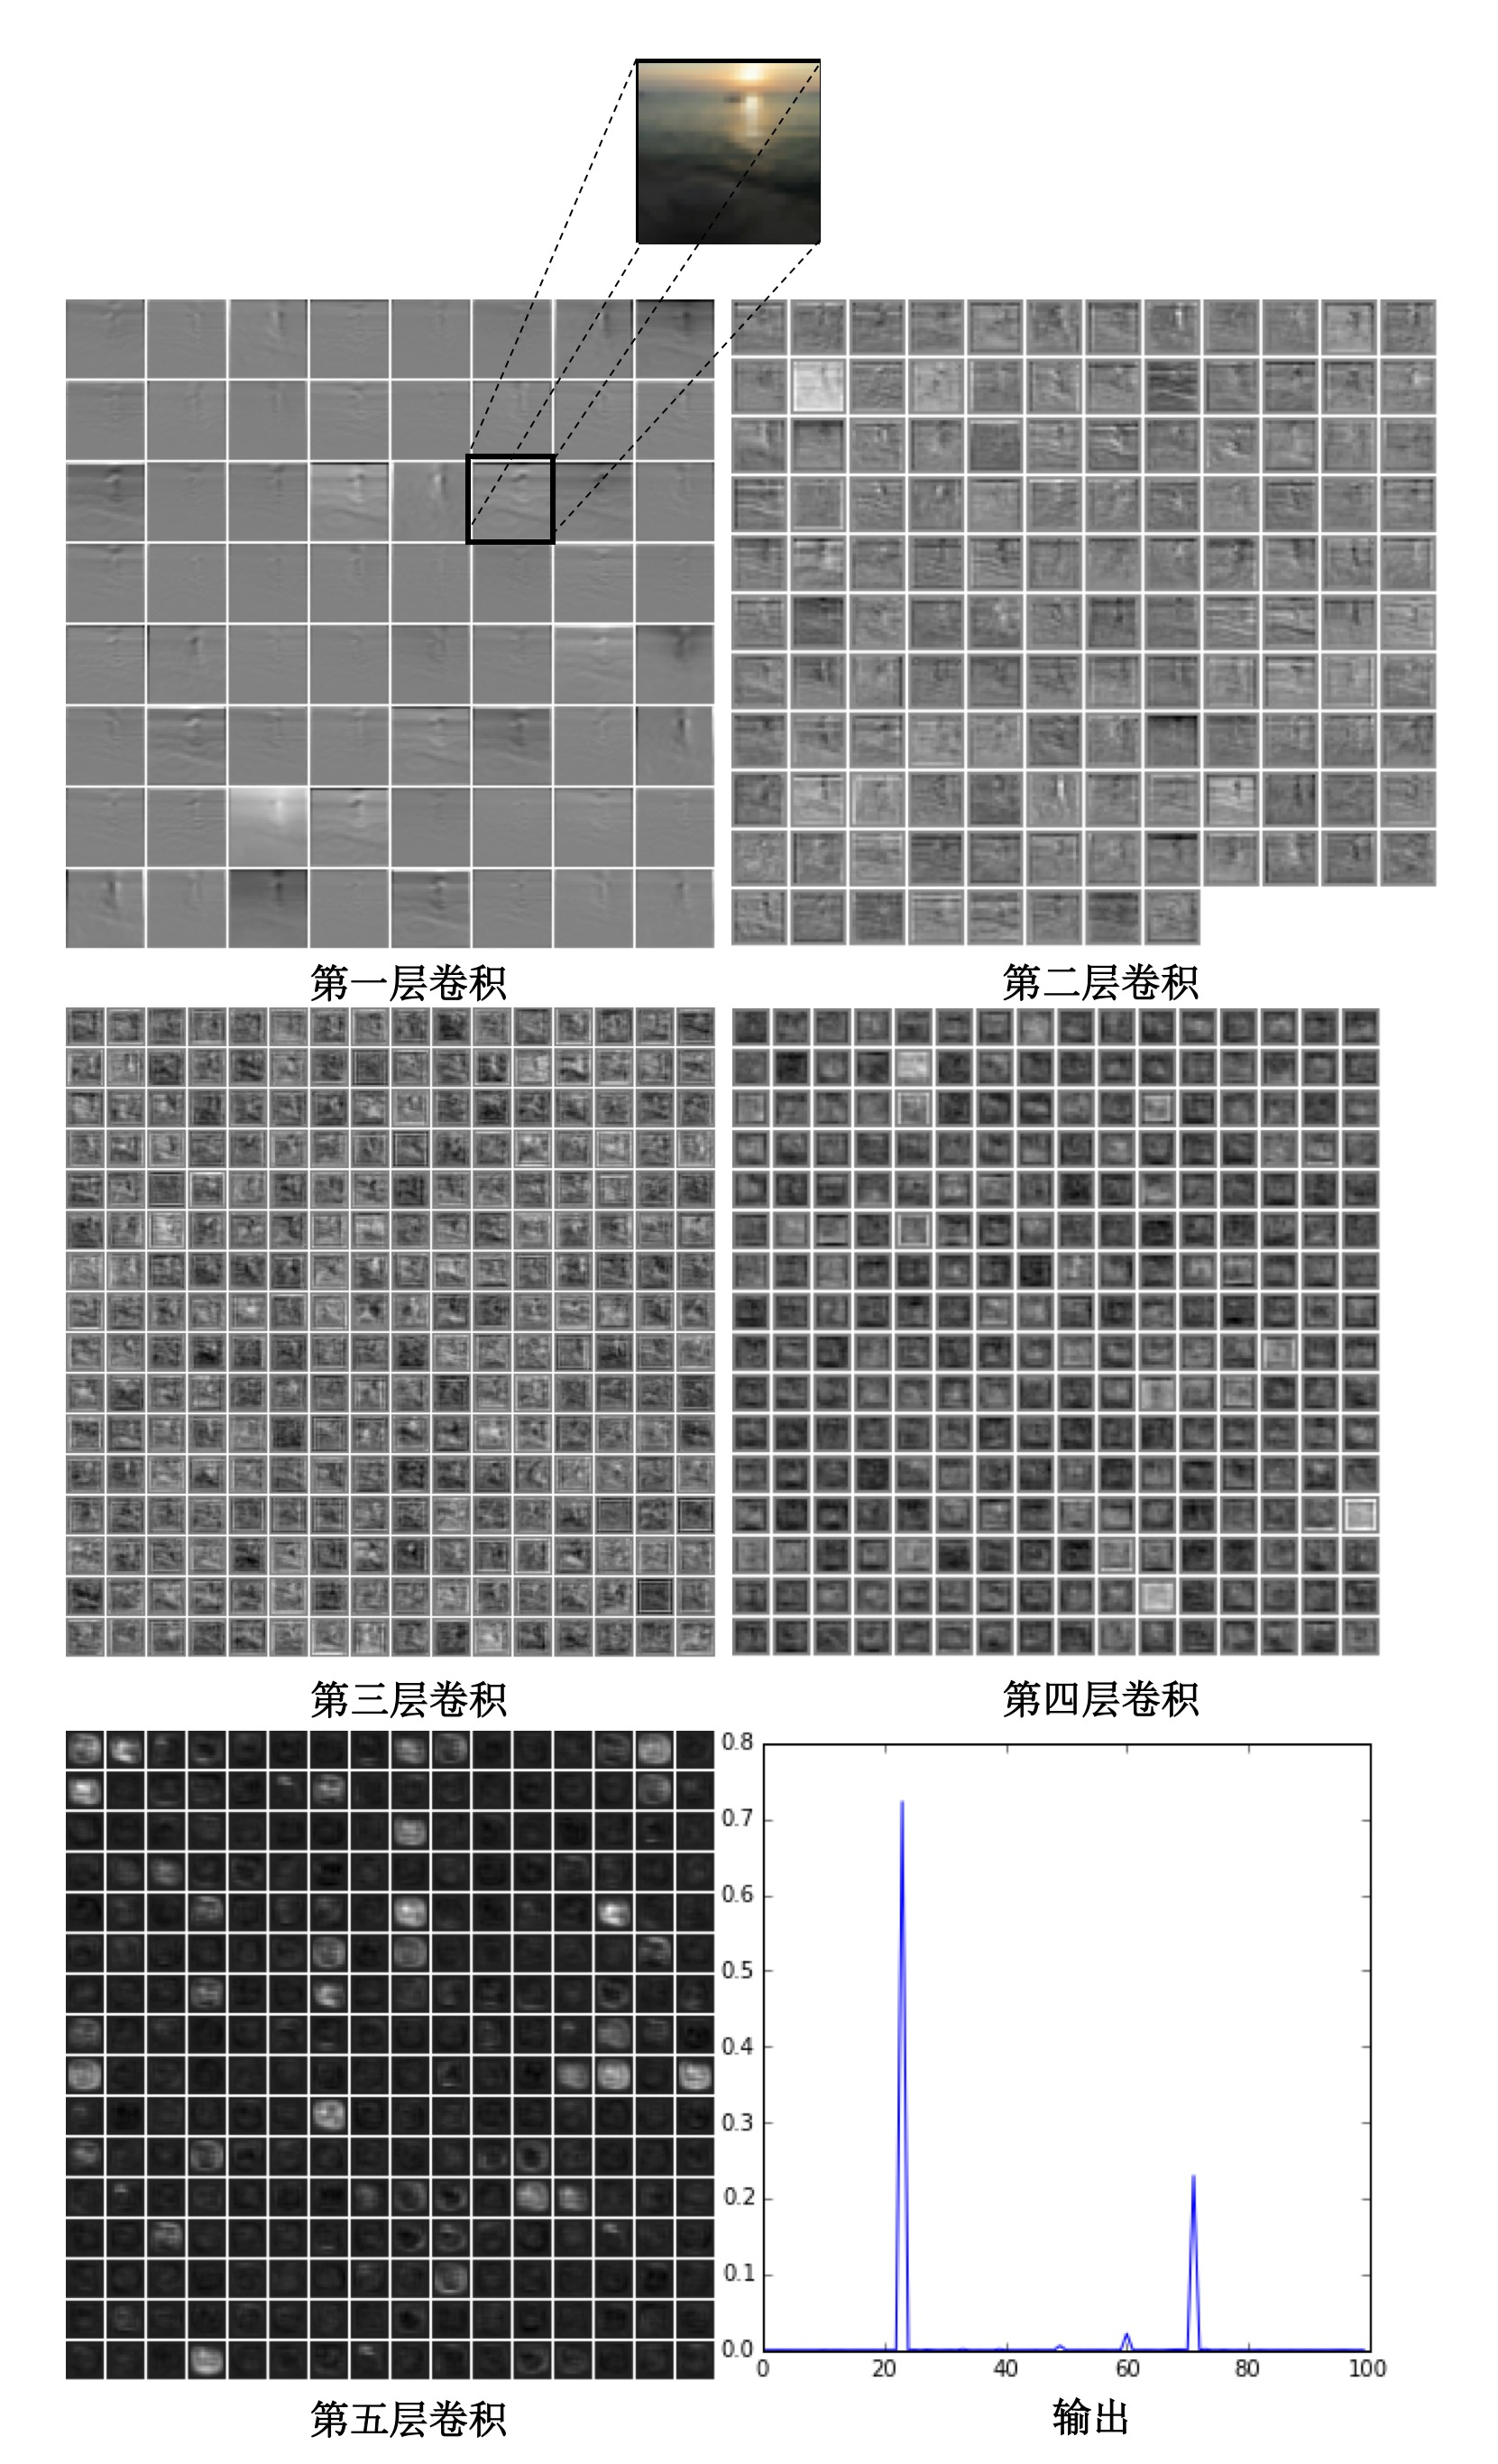
\includegraphics[width=1.0\linewidth]{sam_vis_cifar100.jpg}
\caption{CIFAR-100卷积层特征可视化。}
\label{fig:sam_vis_cifar100}
\end{figure*}

\begin{figure*}
\centering
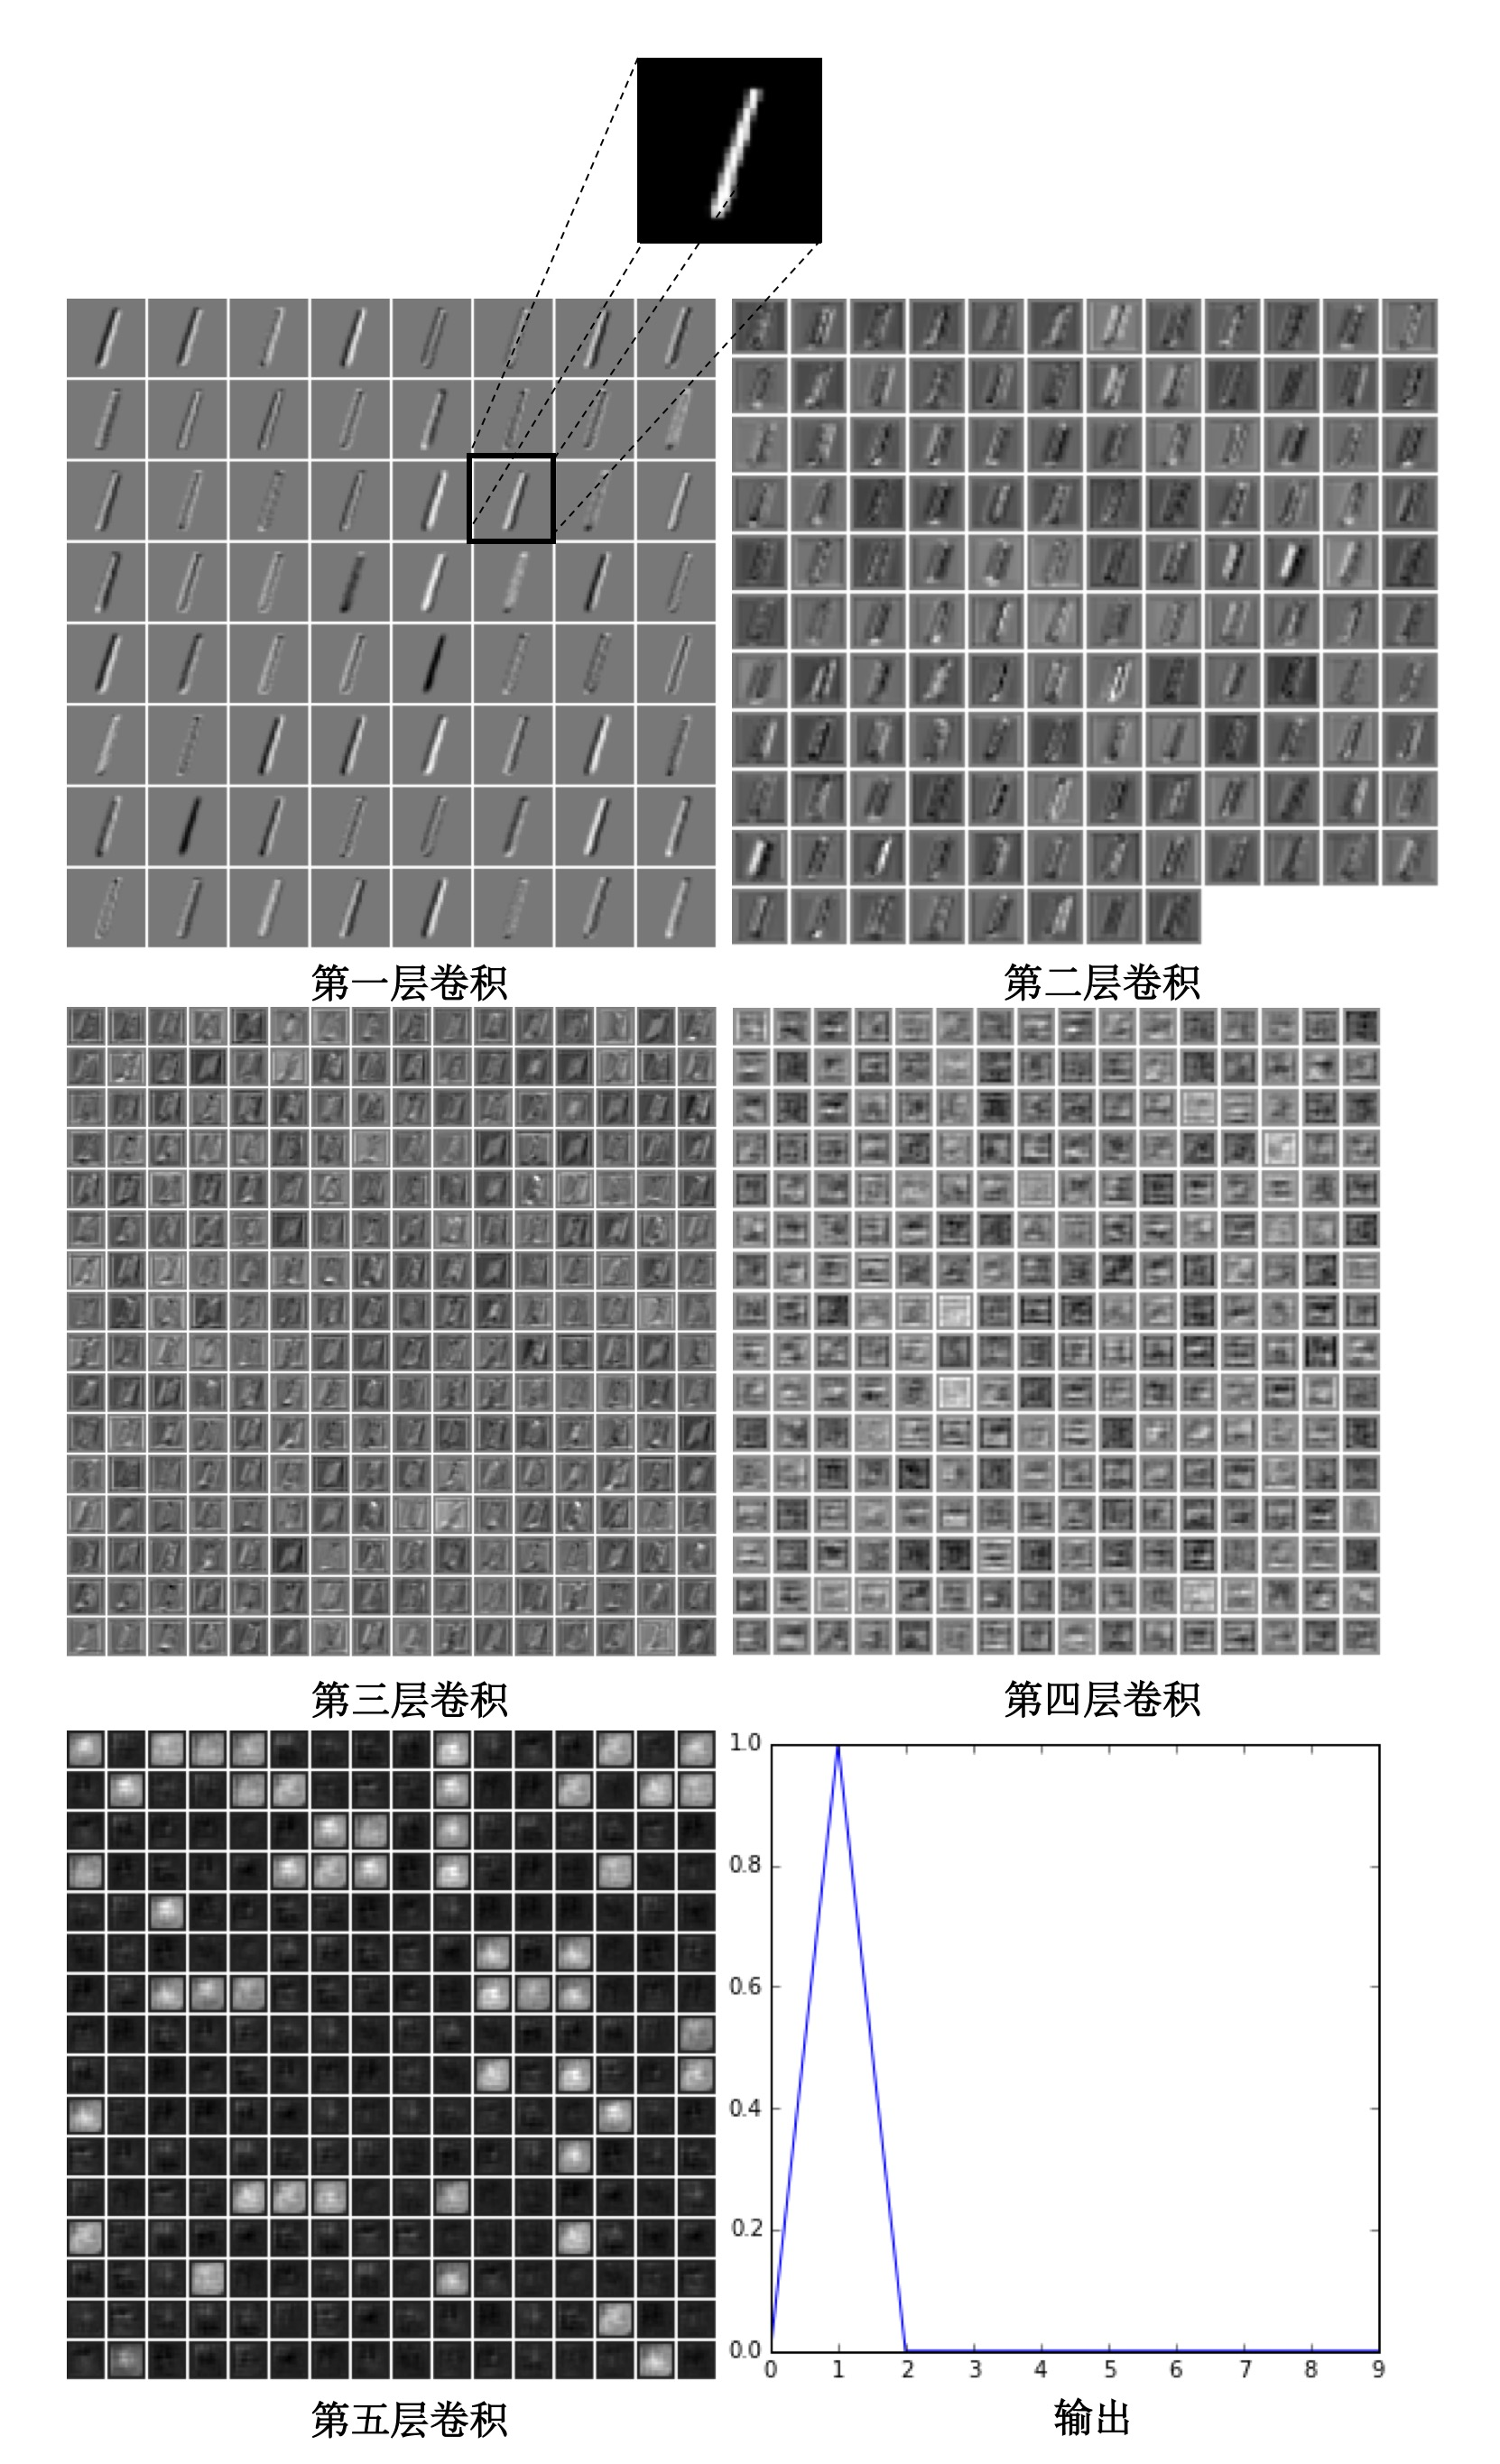
\includegraphics[width=1.0\linewidth]{sam_vis_mnist.jpg}
\caption{MNIST卷积层特征可视化。}
\label{fig:sam_vis_mnist}
\end{figure*}

\begin{figure*}
\centering
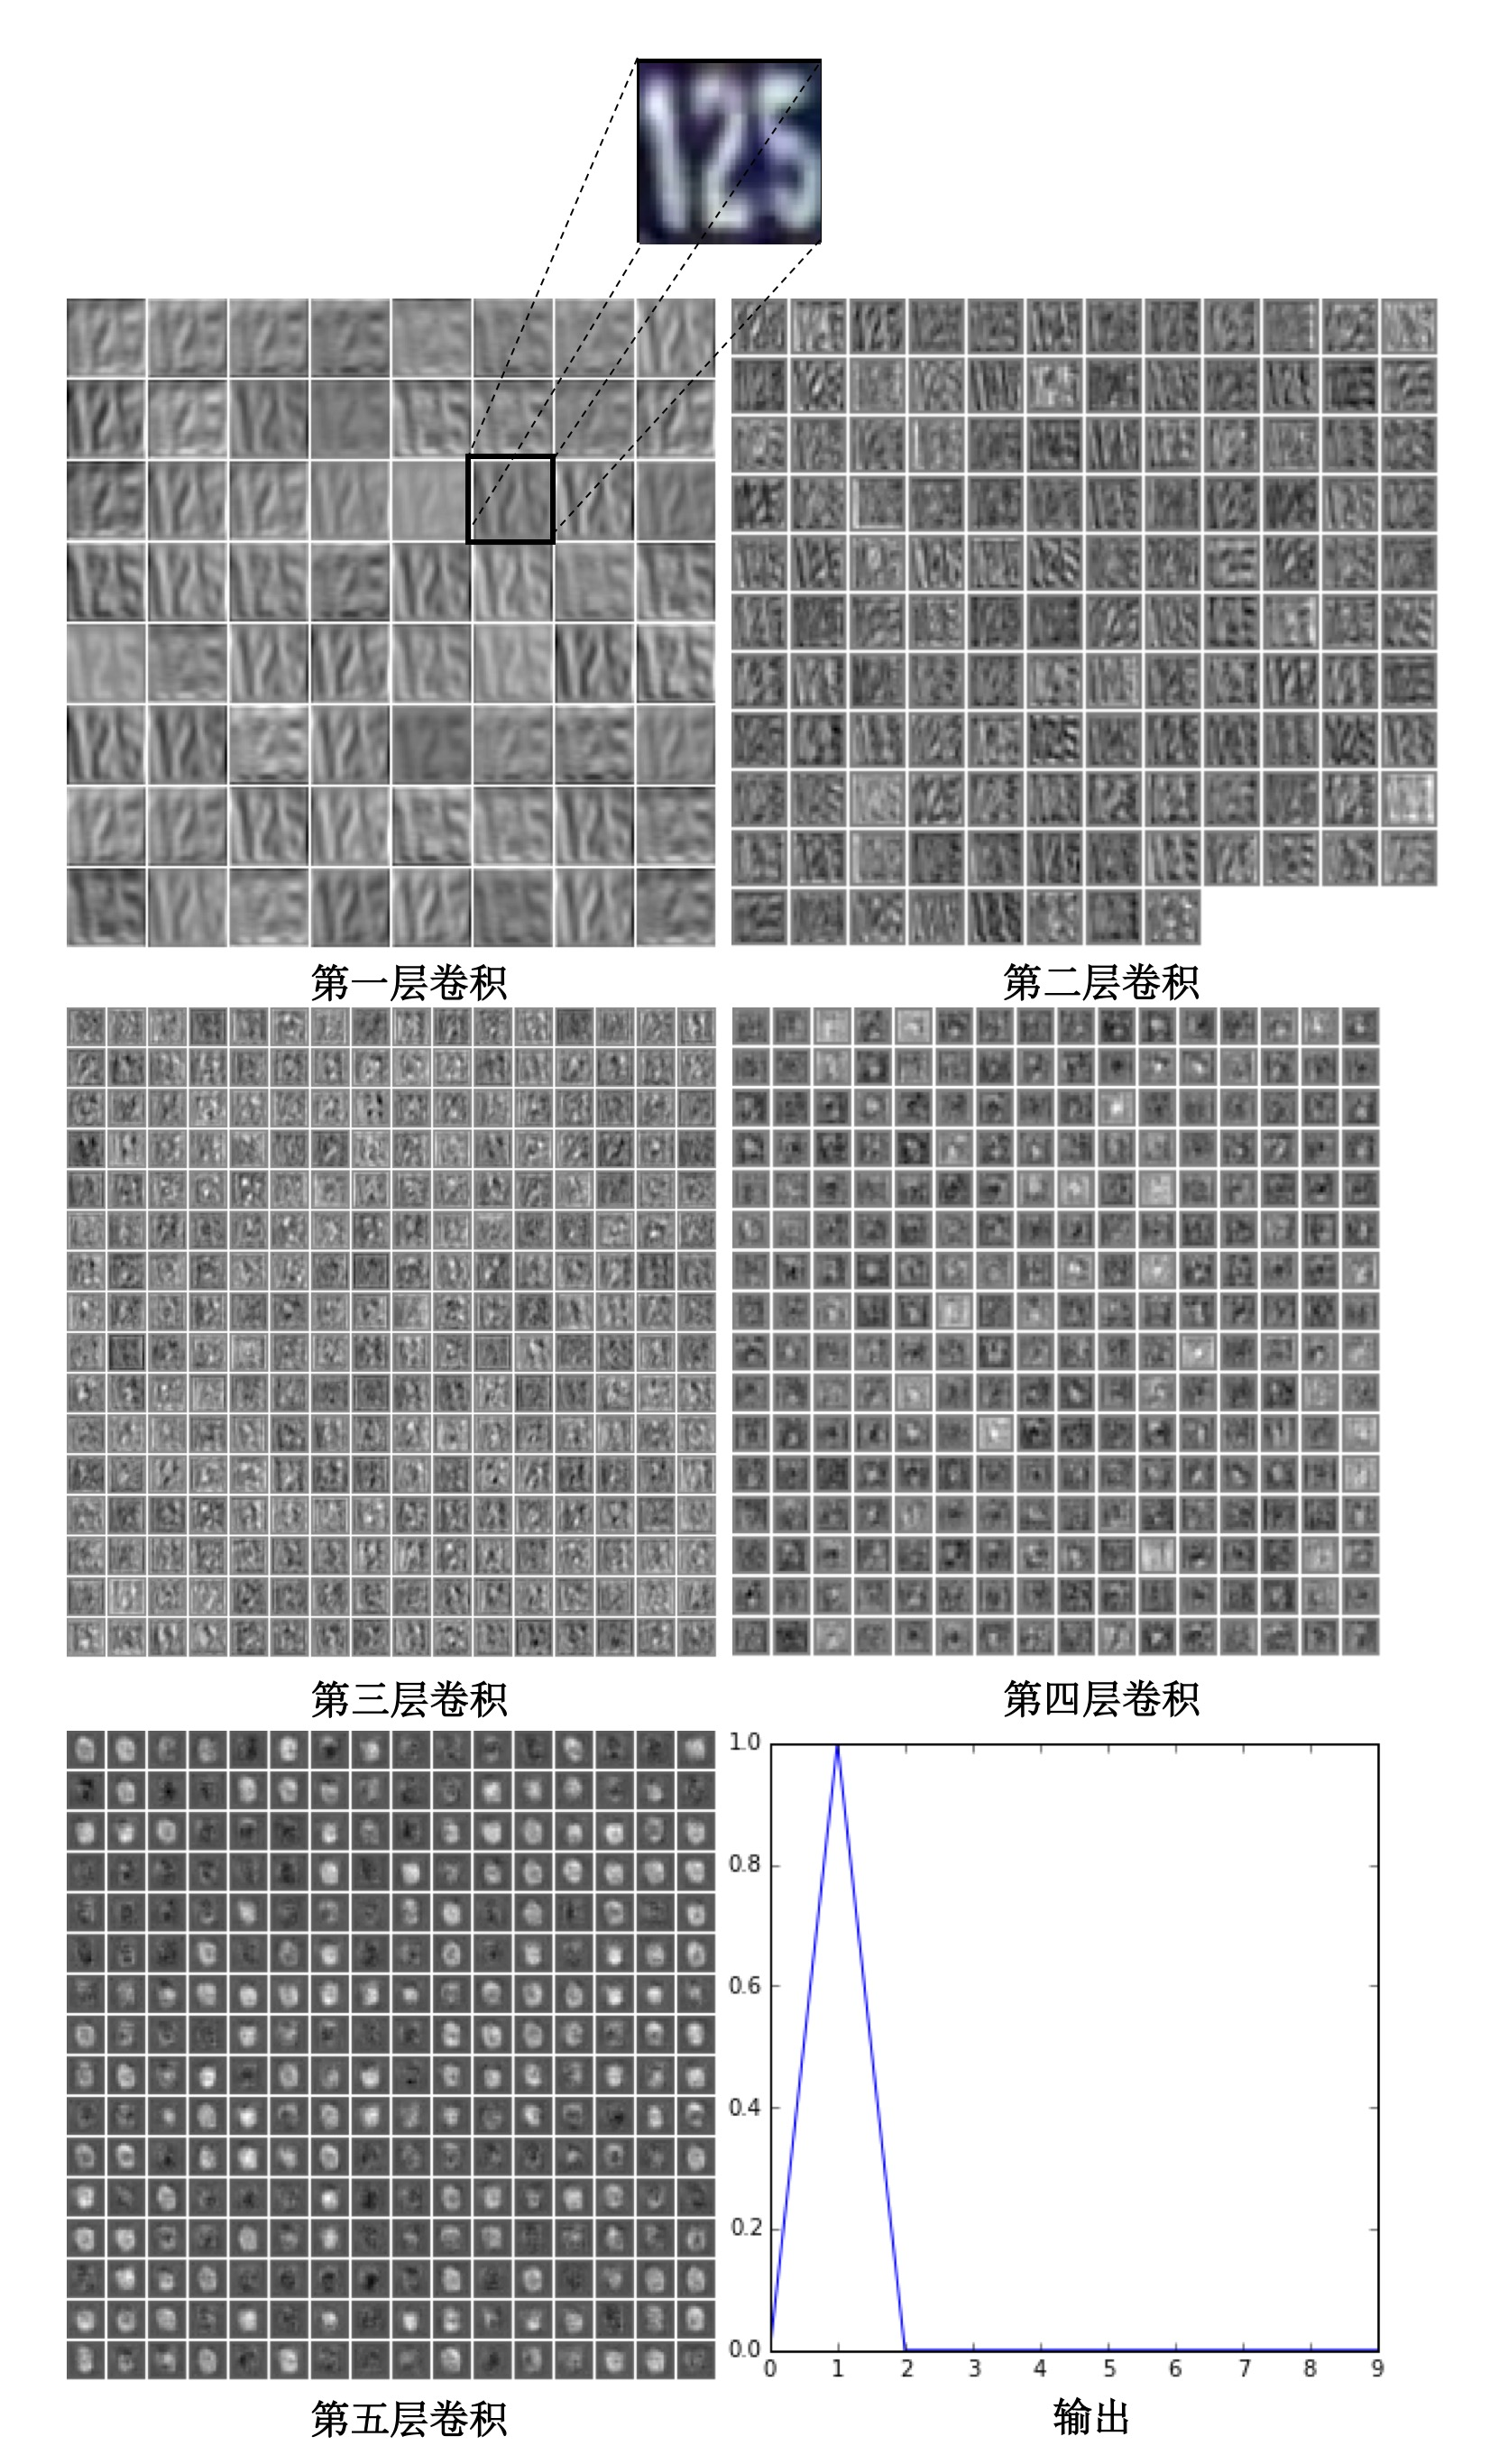
\includegraphics[width=1.0\linewidth]{sam_vis_svhn.jpg}
\caption{SVHN卷积层特征可视化。}
\label{fig:sam_vis_svhn}
\end{figure*}


\begin{figure*}
\centering
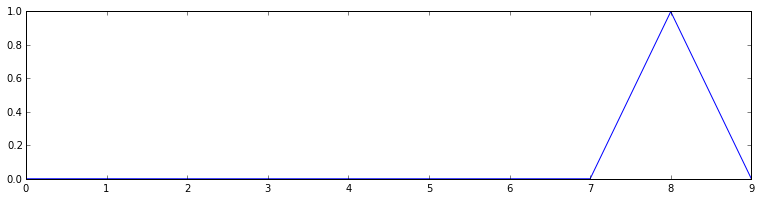
\includegraphics[width=1.0\linewidth]{sam_cifar10_out.png}
\caption{Softmax层各类别预测概率输出。}
\label{fig:sam_cifar10_out}
\end{figure*}

卷积神经网络最后通过Softmax层来预测待识别图像的类别。对于CIFAR-10数据集这样的10分类问题,针对如图~\ref{fig:sam_cifar10_conv1}(a)所示的输入图像,SAMNet的Softmax层输出结果如图~\ref{fig:sam_cifar10_out}所示,SAMNet网络已0.9987的概率预测图~\ref{fig:sam_cifar10_conv1}(a)所属的类别是第8类(即轮船)。

为了增加上述可视化结果的可信度,我们在CIFAR-100、MNIST和SVHN三个数据集上均实现了上述可视化工作,实验结果如图~\ref{fig:sam_vis_cifar100}、图~\ref{fig:sam_vis_mnist}和图~\ref{fig:sam_vis_svhn}所示。其中对于CIFAR-100数据集,我们选了一个分类预测失败的例子,如图~\ref{fig:sam_vis_cifar100}所示。图~\ref{fig:sam_vis_cifar100}中输入样本是海滩,但是网络的预测结果却以0.7226的概率预测为第23类(青蛙)。尽管最终的分类结果有误,但是可以看出浅中层网络提取的特征仍然是图像的边缘与角点等低层特征,且较为清晰准确。此外我们发现,尽管网络最终的预测结果有误,但是网络仍然以一个较高的概率0.2296预测出物体也十分可能是海滩,即该图像的真是类别。可见即使是一个错误的预测概率,也具有很强的先验知识,第四章知识预回归方法即利用了这样的信息。


本章提出的SAMNet可以成功的应用于四个不同的数据集,其中组合卷积结构起到了十分重要的作用。对于相同的网络模型,针对不同的输入数据形式,组合卷积结构采用端到端学习的方式,可以优化得到适用于不同识别任务的特征提取方式,使得SAMNet网络可以在改变网络结构的基础上,在四个数据集上均取得较好的网络泛化能力。


\section{本章小结}
\label{sec:sap:conclusion}

通过有效地结合Inception、Maxout、ResNet和NIN四个网络模型结构,本章提出了一种组合卷积结构:自适应卷积模块,用于简化复杂深度卷积网络的设计过程。SAM以Inception结构为基础计算框架,使SAM可以有效地平衡特征表达能力与计算负荷。SAM主要由四条特征提取分支与一个选择器组成,其中两条卷积分支具有不同的深度和感受野,一条残差分支用于加快SAM结构的收敛速度,一条Maxout分支用于提高SAM结构的非线性拟合能力。选择器具有特征压缩与组合的功能,增强局部感受野范围内的非线性拟合能力。在CIFAR-10、CIFAR-100、MNIST和SVHN四个数据集上,SAMNet分别取得了5.76\%,28.56\%,0.31\%和1.98\%的测试错误率。实验结果表明,使用SAM模块组建卷积神经网络,可以大大简化深度卷积神经网络的设计,同时保持卓越的网络识别性能。
\chapter{随机区域池化}
\label{cha:sap}

\section{引言}
\label{sec:sap:introduction}

对于机器学习算法,特征的表达~\cite{bengio2013representation}具有至关重要的作用,直接反映着对于原始数据统计分布和个体差异的理解。以物体分类为例,有效的特征表达形式,可以极大地简化后端的分类识别算法,提高物体识别率。长期以来,图像的特征提取一般是靠人工设计实现的,虽然已经提出了一些具有不变性(如大小,尺度,旋转,光照等)的特征,如SIFT~\cite{lowe1999object, ke2004pca,ke2004pca},HOG~\cite{dalal2005histograms}和LBP等,并且这些特征在图像的检测识中取得了重要的进展。但是这种设计特征的方法是很困难的,需要很多实验经验、启发,甚至于运气成分,耗时耗力。因此,基于学习的特征提取方法成为人们关注的重点,在过去的几年中,出现了很多较好的研究成果,其中卷积神经网络的研究与发展很大程度上推动了特征学习的研究进展。特别是在2012年Krizhevsky~\cite{krizhevsky2012imagenet}使用深度卷积神经网络模型,通过GPU并行训练的方式,在ImageNet ILSVRC-2010和ILSVRC-2012挑战赛夺冠之后,深度卷积神经网络迎来了一个高速发展的时期。

受生物视觉皮层通路的启发,卷积神经网络采用分层的方式进行特征提取,这也是卷积神经网络可以取得卓越识别性能的一个重要因素。最近几年,大量优秀的网络模型被学者们提出用于解决不同的问题,但是关于卷积神经网络模型的设计,仍然存在着很多尚未解决的问题。比如,如何提高一个卷积神经网络的特征表达能力,使学习到的特征具有更强的分类与识别能力;如何设计出一个通用并且有效的网络模型。本章针对上述两个问题进行了深入的研究。

众所周知,数据増广是一个简单有效提高网络识别能力和泛化能力的技巧。合理的数据増广方式,可以在保证不影响训练图像样本分布的情况下,扩展训练样本空间,增加输入图像的多样性。本章中,我们将数据増广的思想推广到特征空间,即特征层次的数据増广。因此,我们提出了一个新的池化方法,即随机区域池化(Stochastic Area Pooling,SAP),在不改变特征空间样本分布的情况下,扩展特征空间、增加特征的多样性,通过特征増广提高网络的泛化能力,使网络的特征表达能力更加鲁棒。不同于传统的池化方法在一个固定的区域进行池化操作,随机区域池化通过对池化区域进行随机的旋转、平移和缩放,在变换后的池化区域进行池化操作。Jaderberg等人~\cite{jaderberg2015spatial}提出的空间变换网络(Spatial Transformer Network)也采用了特征层的仿射变换。不同之处在于,空间变换网络的仿射变换参数通过学习的方式进行优化;而随机区域池化中变换参数由高斯概率分类随机产生,训练过程中不需要进行优化学习。Jaderberg等人引入一个额外的空间变换网络,通过学习的方式对其进行优化求解,最终生成具有旋转、缩放不变性的特征,整个过程需要学习大量的额外参数,计算量较大。本章提出的随机区域池化通过对特征层进行数据増广,提高网络的泛化能力,基本不会引入额外的网络参数与计算量。

同时,为了避免网络在设计过程中出现表达瓶颈问题~\cite{szegedy2015rethinking},本章提出一个通用卷积神经网络结构,如图~\ref{fig:sap_arc}所示,该结构看起来像一个倒立的T行金字塔,我们称之为T形结构。在T形结构中,与池化层直接相连的卷积层的卷积核翻倍,以此来避免池化过程中特征的过度压缩。此外,对于T形结构中的每个卷积层,我们都统一的以此采用批正则化BN,线性整流单元ReLU,和具有 0.1 丢失比率的Dropout对卷积特征进行后处理。本章所用的所有网络模型都采用了这种T型的网络结构。

本章由随机区域池化和T型结构组成的网络记为SAPNet,我们在四个图像识别数据集上对SAPNet进行了测试,在CIFAR-10~\cite{krizhevsky2009learning},CIFAR-100~\cite{krizhevsky2009learning},MNIST~\cite{lecun1998gradient}和SVHN~\cite{netzer2011reading}上,SAPNet均取得了优越的性能。本章其余内容组织如下:第~\ref{sec:sap:relate}节,回顾了与本章研究内容相关的研究工作;第~\ref{sec:sap:model}节提出了随机区域池化方法和T形网络结构的具体实现;第~\ref{sec:sap:experiment}节详细说明了SAPNet网络结构、参数设置与训练过程,对实验结果进行了必要的分析。最后,在第~\ref{sec:sap:conclude}节是对本章主要内容的总结与概括。

\section{相关工作}
\label{sec:sap:relate}

认知机(Cognitron)~\cite{fukushima1975cognitron} 和神经认知机(Neocognitron)~\cite{fukushima1980neocognitron}通常被认为是最早的卷积神经网络模型,Fukushima在神经认知机计算模型中,提出了诸如卷积、池化、感受野等重要概念,一直沿用至今。1989年,误差的反向传播机制被LeCun等人~\cite{lecun1989backpropagation}引入到神经认知机计算模型中,进一步完善了该模型,衍生出如今的卷积神经网络。

池化是卷积神经网络的一个重要组成部分,它将位置相邻且语义相近的特征规约为一个特征。池化操作可以缩小隐层特征维度,从而降低卷积神经网络的计算量,此外池化在一定程度上增强特征的平移不变性。最常见的池化操作是均值池化(Average Pooling)和最大池化(Max Pooling)~\cite{weng1992cresceptron}。受生物视觉皮层中复杂细胞~\cite{weng1992cresceptron,simoncelli1998model}运行机制的启发,$L_{p}$池化~\cite{hyvarinen2007complex,bruna2013signal}具有更强的泛化能力。Yu等人受Dropout~\cite{hinton2012improving}和DropConnect~\cite{wan2013regularization}启发,提出了混合池化(Mixed Pooling)~\cite{yu2014mixed}方法,有效地结合了最大池化和平均池化两种方法,可以更加有效地解决过拟合问题。类似的,Lee等人~\cite{lee2015generalizing}提出了混合/门式最大均值池化(Mixed/Gate Max-Average Pooling),将混合池化中的随机参数变成一个可学习的参数,通过对池化函数的优化来提高池化的特征表达能力。Zeiler和Fergus~\cite{zeiler2013stochastic}提出了随机池化(Stochastic pooling)方法,根据多项式分布在池化区域内随机选取激活值,采用随机机制来克服过拟合问题。Rippel等人~\cite{rippel2015spectral}采用频率滤波的方式实现特征降维,从而提出了光谱池化(Spectral Pooling)方法。采用线性低通滤波器来实现光谱滤波。与最大池化相比,光谱池化可以保留更多的特征信息。He等人~\cite{he2014spatial}提出了金字塔池化(Spatial Pyramid Pooling,SPP)用于提出多尺度的池化特征,该池化方法对于任意大小的输入图片均可以生成固定长度的特征向量。Gong等人~\cite{gong2014multi}提出了多尺度无序池化(Multi-scale Orderless Pooling ,MOP),在不改变网络识别能力的基础上,增强网络特征不变性。此外,Pu等人~ \cite{pu2015deep}提出随机上采样(Stochastic Unpooling)方法,用于深度生成网络的特征升维。

\section{随机区域池化网络}
\label{sec:sap:model}

本节主要介绍了随机区域池化网络SAPNet的网络结构,SAPNet采用随机区域池化和三个T形结构组成,本小节将分别从这两个主要的组成结构,详细介绍随机区域池化和T形结构的主要实现。

\subsection{随机区域池化层}
\label{sec:sap:model:sap}

\begin{figure} [t]
\centering
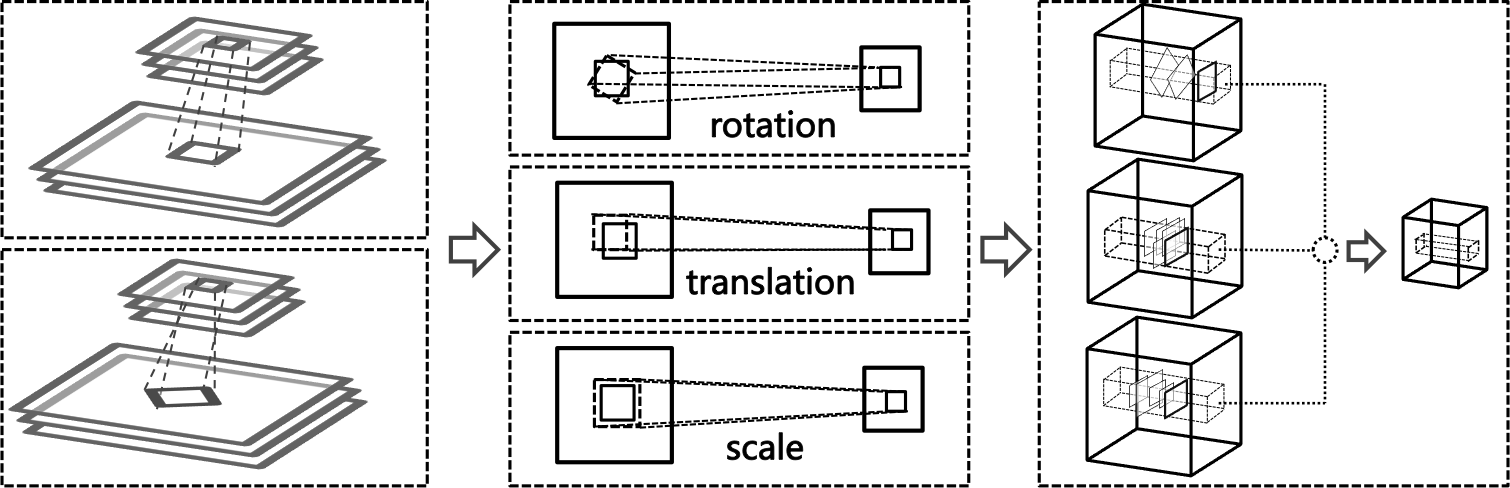
\includegraphics[width=1\linewidth]{sap_sap.png}
\caption{随机区域池化方法。}
\label{fig:sap_sap}
\end{figure}

随机区域池化主要由两个步骤组成:池化区域的选择和池化操作。首先,通过随机仿射变换对池化区域进行重采样。之后,在变换后的池化区域进行池化操作(均值池化、最大池化等),本文采用的是最大池化。

不同于传统的池化方法,在一个固定的正方形区域进行卷积操作,随机区域池化的池化区域通过仿射变换得到:$f : A {\rightarrow} B$,其中 $A {\in} \mathcal{R}^n$ 和 $B {\in} \mathcal{R}^m$ 代表两个仿射空间,假设 $x {\in} A$  代表一个 n 维向量。 仿射变换可以表示为 $f(x) = Tx + b$,其中 $T {\in} \mathcal{R}^{m \times n}$ 为仿射变换矩阵, $b {\in} B$ 为平移向量。对于二维图像空间的仿射变换,本章只考虑了最常见的平移、旋转、缩放变换和它们之间的相互组合形式,用于生成随机区域变化的池化区域。

假设 $\theta$ 代表旋转角,以向量 $[c_x, c_y]$ 为旋转中心, $[o_x, o_y]$ 平移向量,$[s_x, s_y]$ 为缩放因子。 我们可以用一个七元组 $\{\theta, c_x, c_y, o_x, o_y, s_x, s_y\}$ 来表示此仿射变换:
\begin{equation}  \label{equ:all}
  \left[
  \begin{array}{c}
          x' \\
          y' \\
          1
 \end{array}
 \right]
 =
  \left[
  \begin{array}{ccc}
          s_x \cos{\theta} & s_y \sin{\theta} & t_x\\
          -s_y \sin{\theta} & s_x \cos{\theta} & t_y\\
          0 & 0 & 1
  \end{array}
  \right]
  \left[
  \begin{array}{c}
          x \\
          y \\
          1
  \end{array}
  \right]
\end{equation}
\begin{equation} \label{equ:tx}
t_x = c_x (1 - s_x \cos{\theta}) - c_y s_y \sin{\theta} + o_x
\end{equation}
\begin{equation} \label{equ:ty}
t_y = c_x (1 + s_y \sin{\theta}) - c_y s_x \cos{\theta} + o_y
\end{equation}

随机的池化区域通过对上述七元组的随机初始化得到,七元组中每个参数服的概率分布如下:
\begin{equation} \label{equ:theta}
\theta \sim N(0, \sigma_{\theta}), 
\end{equation}
\begin{equation} \label{equ:cx}
c_x, c_y \sim N(0.5d, \sigma_{c})
\end{equation}
\begin{equation} \label{equ:sx}
s_x, s_y \sim N(1, \sigma_{s})
\end{equation}
其中 $d$ 代表输入特征图的高度或宽度;旋转角度、旋转中心、缩放因子分别服从以 0、$0.5d$、0为均值,
$\sigma_{\theta}$、$\sigma_c$ 、$\sigma_s$为标准差的高斯分布。三个标准差的大小直接影响了随机区域池化仿射变换的扰动幅度和特征増广的强度。

对池化区域进行仿射变换,变换后的池化区域往往被映射到非整数的边界上。双线性差值常用于对非整数边界上的特征值进行估计。

在每一轮前向传播的过程中,根据式(\ref{equ:theta}), (\ref{equ:cx}), (\ref{equ:sx})随机生成一组七元组参数。这组参数唯一确定了一组仿射变换的参数和变换后的池化区域,并在此区域进行池化操作,本章采用的是最大池化。反向传播的过程中,前向传播过程中随机生成的七元组和对应的池化区域保持不变,即我们并不对七元组进行参数上的学习与优化,误差按原路进行反向传播。实际上,随机区域池化只是在传统的最大池化基础上,增加了一个随机池化区域仿射变换过程。对池化区域进行随机的仿射变化,在亚像素级别对特征进行重采样,生成一组具有随机平移、旋转和缩放的特征表达,以此来达到特征増广的效果,如图~\ref{fig:sap_sap}所示。

我们仅将随机区域池化用于网络训练阶段,在测试阶段我们令${\sigma_{\theta}=0}$,${\sigma_c=0}$, ${\sigma_s=0}$,即跳过随机区域选择步骤,直接进行池化操作,测试阶段的随机区域池化与最大池化效果相同。这样的设计是为了避免测试阶段随机变量引起测试结果的不确定性。


\subsection{T形卷积网络结构}
\label{sec:sap:model:t}

\begin{figure} [t]
\centering
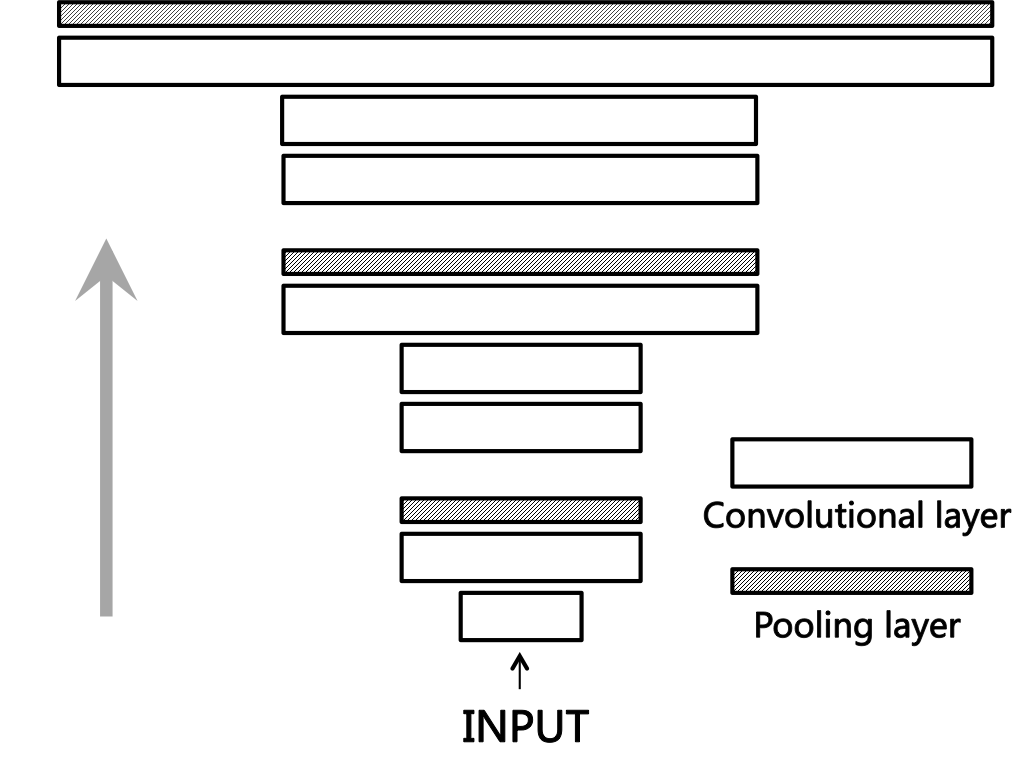
\includegraphics[width=0.7\linewidth]{sap_arc.png}
\caption{T型网络结构。}
\label{fig:sap_arc}
\end{figure}

除池化策略之外,网络结构也会影响特征表达能力。据我们了解,目前的网络结构设计还是经验主义的,并没有系统的理论支持。VGG~\cite{simonyan2014very} 和GoogLeNet~\cite{szegedy2014going,szegedy2015rethinking,szegedy2016inception}的成功启发我们,更深的网络结构、更小的感受野、合适的滑动步长均有助于网络性能的提升。最近He等人~\cite{he2015deep}的实验结果表明,随着网络深度的持续增加,识别精度会趋于饱和甚至下降。Szegedy等人~\cite{szegedy2015rethinking}同时建议,网络的设计应该避免特征表达瓶颈(Representational Bottleneck),特别在网络的初始阶段。实际上,如何确定网络的深度,保证网络的识别能力与计算复杂度;如何有效地组织卷积、池化、非线性化、Dropout层,来实现更优秀的泛化能力;如何设计每个卷积层感受野的大小和卷积核的个数,这些都是值得研究和探索的开放性问题。

\begin{table}[h]
{\caption{SAPNet 网络结构。表中一共定义四个SAPNet网络结构,SAPNet-$N$中的$N$代表与输入图像直接相连的第一个卷积层卷积核的个数。每一个SAPNet都是由三个T型结构、两个随机区域池化、一个全局均值池化、一个全连接层和一个Softmax层组成,八个卷积层被两个随机区域池化均匀隔开。}
\label{tab:model}}
\centering
\begin{tabular}{C{2.5cm}C{2.5cm}C{2.5cm}C{2.5cm}}
 \toprule[1.5pt]
\heiti{SAPNet-16} & \heiti{SAPNet-32} & \heiti{SAPNet-48} & \heiti{SAPNet-64} \\
\midrule[1pt]
conv3-16 & conv3-32 & conv3-48 & conv3-64 \\
conv3-32 & conv3-64 & conv3-96 & conv3-128 \\
\hline
\multicolumn{4}{c}{随机区域池化层} \\
\hline
conv3-32 & conv3-64 & conv3-96 & conv3-128 \\
conv3-32 & conv3-64 & conv3-96 & conv3-128 \\
conv3-64 & conv3-128 & conv3-192 & conv3-256 \\
\hline
\multicolumn{4}{c}{随机区域池化层} \\
\hline
conv3-64 & conv3-128 & conv3-192 & conv3-256 \\
conv3-64 & conv3-128 & conv3-192 & conv3-256 \\
conv3-128 & conv3-256 & conv3-384 & conv3-512 \\
\hline
\multicolumn{4}{c}{全局均值池化} \\
\hline
\multicolumn{4}{c}{全连接层} \\
\hline
\multicolumn{4}{c}{Softmax层} \\
 \bottomrule[1.5pt]
\end{tabular}
\end{table}

本节中,我们精心设计了一个通用的T形卷积网络结构,如图~\ref{fig:sap_arc} 所示。我们用长条状的立方体表示卷积层,立方体的长度代表卷积核的个数。不同于VGG结构在同一个阶段采用相同的卷积核数量进行分层的特征提取,T形结构中与池化层相连的卷积层卷积核个数会翻倍,此结构看起来像一个T型的倒金字塔,我们称之为T型网络结构。采用第~\ref{sec:sap:model:sap} 节随机区域池化和T型结构,我们构造了SAPNet,如表~\ref{tab:model} 所示。表~\ref{tab:model} 中,我们一共定义四个SAPNet网络结构,SAPNet-$N$中的$N$代表与输入图像直接相连的第一个卷积层卷积核的个数。每一个SAPNet都是由三个T型结构、两个随机区域池化、一个全局均值池化、一个全连接层和一个Softmax层组成,八个卷积层被两个随机区域池化均匀隔开。第一个T型结构中仅包换两个卷积层,这是因为相对于其他特征层,输入图片的尺寸最大,出于减少计算量的角度考虑,在第一个T型结构中去掉了一层卷积。

在SAPNet中,所有的卷积都采用 $3\times3$ 大小的感受野,1 个像素的填充,1 个像素的卷积滑动步长,这样的配置可以保持卷积后的特征尺寸保持不变。在随机区域池化层,我们采用 $2\times2$ 的池化区域大小和 2 个像素的池化窗口滑动步长。最后一个卷积层之后,采用全局均值池化来提取固定维度长度的特征。与其他图像识别任务相似地,我们也采用Softmax层作为各类别的预测概率。此外,对于所有的卷积层,我们依次采用批正则化BN~\cite{ioffe2015batch}对特征进行正则化处理,线性整流单元ReLU作为非线性激活函数,具有 0.1 丢弃率的Dropout来防止网络过早的进入过拟合。本章采用的BN操作与原论文~\cite{ioffe2015batch}的略有不同,我们忽略了原文中BN的比例和平移操作,我们仅仅将BN作为对卷积特征的一种正则化。

\begin{table*}
\centering
\caption{不同深度的卷积神经网络在CIFAR-10上的性能对比。“网络结构”是对不同卷积网络结构的缩写。 例如 '2331' 指该网络结构为 8(2+3+3)个卷积层和 1 个全连接层,被 3 个最大池化分隔成 4 个部分,每个部分具有 2,3,3 个卷积层和 1 个全连接层,最后一个池化层是全局最大池化,提取具有固定长度的特征,最后通过Softmax来预测各类别的预测概率。}
\label{tab:layers}
\begin{tabular}{C{2.8cm}|C{0.9cm}C{0.9cm}C{0.9cm}C{0.9cm}C{0.9cm}C{0.9cm}C{0.9cm}C{0.9cm}C{1.cm}}%{c|ccccccccc}
 \hline
{\heiti 层数} & 6 & 7 & 8 & 9 & 10 & 11 & 12 & 13 & 14 \\
\hline
{\heiti 网络结构} & 2221 & 2321 & 2331 & 2431 & 2441 & 2541 & 2551 & 2651 & 2661\\
\hline
{\heiti 测试误差率 (\%)} & 10.09 & 8.77 & 8.53 & 8.35 & 7.93 & \bf{7.65} & 7.86 & 7.63 & 7.77\\
\hline
{\heiti 网络感受野} &  32 & 36 & 44 & 48 & 56 & 60 & 68 & 72 & 80\\
\hline
{\heiti 参数规模 (百万)} & 0.57 & 0.61 & 0.76 & 0.80 & 0.94 & 0.98 & 1.13 & 1.16 & 1.31 \\
\hline
\end{tabular}
\end{table*}

对于网络深度的选择,我们在CIFAR-10上进行了一组实验,实验结果如表~\ref{tab:layers} 所示。如果不算全连接层,本章采用的SAPNet(如表~\ref{tab:model}所示) 网络深度为八。深度为八的网络并不是表~\ref{tab:layers} 中错误率最低的,但是综合考虑网络的识别率、计算量和参数数量,可以看出具有 8-11 层卷积的网络模型都是一个合适的选择,而八层网络具有最少的计算规模和参数数量,因此本章的大部分实验都是基于八层卷积网络模型展开的。从表~\ref{tab:layers} 我们还可以看出,网络深度的选择与网络的感受野存在一定的关系。随着网络深度的增加,网络的感受野也逐渐增大,当网络的感受野增大到输入图片的 1.5-2.0 倍的时候,网络的识别能力达到峰值。继续增加网络的深度,对网络识别能力影响不大,额外增加的计算量与可学习参数并没有带来更高的回报与收益。在CIFAR-10,CIFAR-100,MNIST和SVHN这四个数据集上,输入图像的大小为$32\times32$ 或 $28\times28$,一个 8-11 层卷积的网络模型足以获取优越的识别性能。

为了解决特征瓶颈~\cite{szegedy2015rethinking}的问题,我们通过增加特征的通道数来缓解特征尺度上的锐减。特征的维度可以表示为特征的通道数与每张特征图的分辨率的乘积。一般情况下,从输入图像到最后一个卷积层,特征的维度应该缓慢的进行缩减。也就是说,我们应该避免特征维度大幅度的急剧压缩,以防止特征信息的快速流失。考虑到池化操作不会影响特征的通道数,但会成倍缩小特征图的分辨率,如果采用步长为2的滑动窗口进行池化,特征图分辨率会减小到原来的 $1/4$。由此可见,池化很有可能会导致特征因大幅压缩而出现特征的过度流失,产生特征瓶颈问题。为了克服这个现象,我们提出了T型网络结构,通过增加与池化层直接相连的卷积层中卷积核的个数,来增加池化前特征的通道数,尽量降低池化过程中特征的信息流失。

SAPNet网络在设计的过程中,需要考虑的另一个问题是如何合理的分配网络的计算复杂度。卷积神经网络的大部分计算集中在卷积操作,而决定卷积层计算量的主要是输入特征的维度和卷积参数。在池化前后,合理的分配输入输出特征图的通道数,可以有效地平衡网络的不同阶段的计算量。

\subsection{分析与讨论}
\label{sec:sap:model:discuss}

本章我们提出了一个由随机区域池化和T形网络结构组成的SAPNet网络用于图像识别任务,该网络主要由两个随机区域池化与三个T型网络结构搭建而成。

受数据増广的启发,为了提高网络的泛化能力,我们将数据増广推广到特征层,提出了随机区域池化方法。通过随机放射变换对池化区域进行扰动,生成一组具有平移、旋转和缩放的特征表达,扩大了特征的样本空间,增加了特征的多样性。随机区域池化方法并不需要优化仿射变换参数,整个计算过程十分简单快速,并未引入过多的额外计算开销,是一种计算代价很小的提升网络泛化能力的方法。值得注意的是,随机区域池化并不是一种增强特征不变性的方法,而是通过特征増广来增强网络泛化能力,防止网络过早进入过拟合的方法。本章中采用最大池化对随机区域内的特征进行规约,相当于在最大池化的技术上,对输出特征进行了合理的扰动。同样地,均值池化也可以与随机区域选择相配合,达到特征増广的效果。

此外,我们设计T型网络结构,并以此设计了SAPNet网络。不同于其他网络模型仅仅在全连接层使用Dropout,我们在每个卷积层都采用一个丢失率较小的Dropout对特征进行正则化,防止网络过早地进入过拟合状态。实验结果表明,这样的配置可以保证网络的稳定性和泛化能力。


\section{实验结果}
\label{sec:sap:experiment}

基于caffe~\cite{jia2014caffe}深度学习框架,我们实现了本章提出的随机区域池化和T型网络模型。所有的实验都以数据并行的方式运行于具有两颗GPU核心的高性能服务器。我们在四个图像识别数据集CIFAR-10,CIFAR-100,MNIST,和SVHN上对多组不同参数大小的SAPNet进行了测试,我们在CIFAR-10数据集上,设计了更多的对比实验来验证本章随机区域池化和T型网络结构的有效性。

在所有实验中,我们批大小(Batch Size)为 96 的随机随机梯度下降算法训练网络。网络的初始学习率为 0.01,网络训练过程中学习率会逐渐减小,每次缩小为原来的 $1/10$,持续缩小3次,直到学习率降低到 1e-5。网络训练过程中,采用 0.9 的动量因子(Momentum)和 0.004 的权重衰减因子(Weight Decay )对参数进行更新。对于随机区域池化层,各参数的标准差设为$\sigma_{\theta}=5^{\circ}$,$\sigma_c=0.25d$,$\sigma_s=0.01$。采用与第~\ref{sec:sap:experiment:param}节相同的数据预处理方式,即对于每张图片,逐像素减去训练图像对应位置的像素BGR均值。

\subsection{CIFAR-10}
\label{sec:sap:cifar10}

我们首先在CIFAR-10~\cite{krizhevsky2009learning}数据集上验证随机区域池化与T型网络的有效性。CIFAR-10由 60,000 张 $32\times32$ 大小的 10 类彩色图像构成,整个数据集被平均分成 6 份,每份 10,000 张图片,其中 5 份作为训练数据,1 份作为测试数据。

\begin{table}[h]
\centering
\caption{随机区域池化与其他池化方法的对比试验。表中我们对最大池化、均值池化、随机池化进行了对比实验,结果可以看出,在网络的泛化能力上,随机区域池化 > 均值池化 > 随机池化 > 最大池化。}
\label{tab:others}
%\begin{tabular}{C{3cm}C{2cm}C{2cm}}
 \begin{tabular}{lcc}
 \toprule[1.5pt]
{\heiti 模型} & {\heiti 参数规模} & {\heiti 测试错误率(\%)} \\
\midrule[1pt]
SAPNet-32(最大池化) & 0.76 M & 8.53 \\
SAPNet-32(均值池化) & 0.76 M & 8.13 \\
SAPNet-32(随机池化) & 0.76 M & 8.50 \\
\hline
SAPNet-32(随机区域池化) & 0.76 M & \bf{7.56} \\
 \bottomrule[1.5pt]
\end{tabular}
\end{table}

\begin{table}[b]
\centering
\caption{不同参数规模下随机区域池化与最大池化性能对比。SAPNet-32(随机区域池化)的性能要好于比它的参数规模与计算量大一倍的SAPNet-48(最大池化);SAPNet-48(随机区域池化)的性能与比它的规模大近一倍的SAPNet-64(最大池化)基本持平。}
\label{tab:max}
%\begin{tabular}{C{3cm}C{2cm}C{2cm}}
\begin{tabular}{lcc}
 \toprule[1.5pt]
{\heiti 模型} & {\heiti 参数规模} & {\heiti 测试错误率(\%)} \\
\midrule[1pt]
SAPNet-32(最大池化) & 0.76 M & {8.53} \\
SAPNet-48(最大池化) & 1.71 M &{7.69} \\
SAPNet-64(最大池化) & 3.03 M & {7.01} \\
\hline
SAPNet-32(随机区域池化) & 0.76 M & {7.56} \\
SAPNet-48(随机区域池化) & 1.71 M &{7.02} \\
SAPNet-64(随机区域池化) & 3.03 M & {6.61} \\
 \bottomrule[1.5pt]
\end{tabular}
\end{table}

随机区域池化与其他池化方法的对比结果如表~\ref{tab:others} 所示。实验中,我们采用了与SAPNet-32(表~\ref{tab:model})相同的八层卷积网络结构,分别用最大池化、均值池化、随机池化来替换SAPNet-32中的随机区域池化。在没有数据増广的情况下,表~\ref{tab:others} 中所有的实验都达到了一个极高的识别率。在相同的网络结构、参数规模和计算量的基础上,随机区域池化方法明显好于最大池化、均值池化和随机池化。从本次实验的结果可以看出,对于网络的泛化能力上,随机区域池化 > 均值池化 > 随机池化 > 最大池化。由此可见,相对于最大池化、均值池化和随机池化,随机区域池化可以有效地增强网络的泛化能力,提升网络的测试性能。


\begin{table}[!h]
\centering
\caption{CIFAR-10数据集上与已有模型的对比实验。}
\label{tab:cifar10}
%\begin{tabular}{C{4.5cm}C{1cm}C{2cm}}
\begin{tabular}{L{6cm}cc}
 \toprule[1.5pt]
{\heiti 模型} & {\heiti 参数规模} & {\heiti 测试错误率(\%)} \\
\midrule[1pt]
\multicolumn{3}{c}{\heiti 没有数据増广} \\
\hline
Maxout~\cite{goodfellow2013maxout} & $>$5 M & 11.68 \\
Prob maxout~\cite{springenberg2013improving} & $>$5 M & 11.35 \\
DasNet~\cite{stollenga2014deep} &  $>$5 M & 9.22 \\
NIN~\cite{DBLP:journals/corr/LinCY13} & 0.97 M & 10.41 \\
DSN~\cite{lee2015deeply} & 0.97 M &9.69 \\
%RCNN-96~\cite{liang2015recurrent} & 0.67 M & 9.31 \\
%RCNN-128~\cite{liang2015recurrent} & 1.19 M & 8.98 \\
RCNN~\cite{liang2015recurrent} & 1.86 M & {8.69} \\
ALL-CNN~\cite{springenberg2015striving} & 1.3 M & 9.08 \\
Tree+Max-Avg~\cite{lee2015generalizing} & 1.85M & \bf{7.62} \\
\hline
SAPNet-32 & 0.76 M & \bf{7.56} \\
SAPNet-48 & 1.71 M &\bf{7.02} \\
SAPNet-64 & 3.03 M & \bf{6.36(6.50$\pm$0.14)} \\
\midrule[1pt]
\multicolumn{3}{c}{\heiti 有数据増广} \\
\hline
Maxout~\cite{goodfellow2013maxout} & $>$5 M & 9.38 \\
Prob maxout~\cite{springenberg2013improving} & $>$5 M & 9.39 \\
dasNet~\cite{stollenga2014deep} &  $>$5 M & 9.22 \\
DropConnect~\cite{wan2013regularization} & 5 networks & 9.32 \\
NIN~\cite{DBLP:journals/corr/LinCY13} & 0.97 M & 8.81 \\
DSN~\cite{lee2015deeply} & 0.97 M & 7.97 \\
%RCNN-96~\cite{liang2015recurrent} & 0.67 M & 7.37 \\
%RCNN-128~\cite{liang2015recurrent} & 1.19 M & 7.24 \\
RCNN~\cite{liang2015recurrent} & 1.86 M & 7.09 \\
Highway network~\cite{srivastava2015training} & 2.3 M & 7.54(7.72$\pm$0.16) \\
ALL-CNN~\cite{springenberg2013improving} & 1.3 M & 7.25 \\
%ResNet-20~\cite{he2015deep} & 0.27 M & 8.75 \\
%ResNet-32~\cite{he2015deep} & 0.46 M & 7.51 \\
%ResNet-44~\cite{he2015deep} & 0.66 M & 7.17 \\
%ResNet-56~\cite{he2015deep} & 0.85 M & 6.97 \\
ResNet~\cite{he2015deep} & 1.7M & {6.43(6.61$\pm$0.16)} \\
Fitnet4-LSUV~\cite{mishkin2015all} & 2.5M & 6.06 \\
Tree+Max-Avg~\cite{lee2015generalizing} & 1.85M & \bf{6.05} \\
Tuned CNN~\cite{snoek2015scalable} & 1.29M & 6.37 \\
\hline
SAPNet-32 & 0.76 M & {6.77} \\
SAPNet-48 & 1.71 M & \bf{5.92} \\
SAPNet-64 & 3.03 M & \bf{5.57(5.66$\pm$0.09)} \\
\midrule[1pt]
\multicolumn{3}{c}{\heiti 超大规模数据増广} \\
\hline
Large ALL-CNN~\cite{springenberg2014striving} & - & 4.41 \\
Fractional MP~\cite{graham2014fractional} & - & \bf{3.47} \\
 \bottomrule[1.5pt]
\end{tabular}
\end{table}

为了更直观地理解随机区域池化对网络泛化能力的提升幅度,我们进行了多组随机区域池化与最大池化的对比实验,如表~\ref{tab:max} 所示。在具有相同网络结构、参数规模和计算复杂度的情况下,随机区域池化均优于最大池化。并且一个有趣的发现是,SAPNet-32(随机区域池化)的性能要好于比它的参数规模与计算量大一倍的SAPNet-48(最大池化);SAPNet-48(随机区域池化)的性能与比它的规模大近一倍的SAPNet-64(最大池化)基本持平。由此可见,采用随机区域池化的性能提升,已经近似于为网络增加了接近一倍的额外参数与计算量所能达到的效果。


最后,我们对比了SAPNet与其他曾经在CIFAR-10上取得过优异成绩的公开模型,实验结果如表~\ref{tab:cifar10}所示。我们对三组具有不同参数规模的SAPNet进行了测试,在没有数据増广的情况下,三组模型的测试错误率均优于已有的模型。即使是参数规模最小的SAPNet-32,具有大约 0.76 M 参数,性能依然超越了Tree+Max-Avg~\cite{lee2015generalizing}的性能。SAPNet-64以6.36\%的测试错误率,在没有数据増广的情况下,在CIFAR-10数据集上取得了最好结构。为了避免单次实验的偶然性,我们对SAPNet-64重复测试了五次,以保证实验结果的可靠。


特征増广与数据増广是两个不同的概念,对于采用了随机区域池化的网络模型,数据増广依然有效,可以进一步提高网络的识别率。为此,我们增加了多组在具有数据増广情况下CIFAR-10数据集的实验结果,如表~\ref{tab:cifar10} 所示。与之前的工作~\cite{goodfellow2013maxout,springenberg2013improving,stollenga2014deep,wan2013regularization,DBLP:journals/corr/LinCY13,lee2014deeply,liang2015recurrent,srivastava2015training,springenberg2014striving}相同,我们通过随机平移和水平翻转对CIFAR-10数据集的训练图像进行数据増广。测试时,从测试图像的四角和中心分别截取 $24\times24$ 像素大小的五张图片,并对其进行水平翻转,即对一共十张图片进行测试,最终的测试结果是十张图片预测概率的均值。实验结果如表~\ref{tab:cifar10} 所示,在具有数据増广的情况下,SAPNet-64以5.57\%的测试错误率,超越了Tree+Max-Avg~\cite{lee2015generalizing}。

\begin{table}[t]
\begin{center}
\caption{CIFAR-100数据集上与已有模型的对比实验。}
\label{tab:cifar100}
\begin{tabular}{L{6cm}cc}
 \toprule[1.5pt]
{\heiti 模型} & {\heiti 参数规模} & {\heiti 测试错误率(\%)} \\
\midrule[1pt]
\multicolumn{3}{c}{\heiti 没有数据増广} \\
\hline
Maxout~\cite{goodfellow2013maxout} & $>$5 M & 38.57 \\
Prob maxout~\cite{springenberg2013improving}  & $>$5 M & 38.14 \\
DasNet~\cite{stollenga2014deep} & $>$5 M & 33.78 \\
Tree based priors~\cite{srivastava2013discriminative} & - & 36.85 \\
NIN~\cite{DBLP:journals/corr/LinCY13} & 0.98 M & 35.68 \\
DSN~\cite{lee2015deeply}  & 0.98 M & 34.57 \\
%RCNN-96~\cite{liang2015recurrent} & 0.67 M & 34.18 \\
%RCNN-128~\cite{liang2015recurrent} & 1.19 M & 32.59 \\
RCNN~\cite{liang2015recurrent}  & 1.87 M & {31.75 }\\
ALL-CNN~\cite{springenberg2013improving} & 1.30 M & 33.71 \\
Tree+Max-Avg~\cite{lee2015generalizing} & 1.76 M & 32.37 \\
ELU-Network~\cite{clevert2015fast} & 39.32 M & \bf{24.28} \\
\hline
SAPNet-32 & 0.76 M & {32.22} \\
SAPNet-48 & 1.71 M &{29.32} \\
SAPNet-64 & 3.03 M & \bf{27.59} \\
\midrule[1pt]
\multicolumn{3}{c}{\heiti 具有数据増广} \\
\hline
Highway Network~\cite{srivastava2015training} & 2.30 M & 32.24 \\
Fitnet4-LSUV~\cite{mishkin2015all} & 2.5 M & 27.66 \\
Tuned CNN~\cite{snoek2015scalable} & 1.29 M & 27.40 \\
\hline
\multicolumn{3}{c}{{\bf{Extreme}} data augmentation} \\
\hline
Fractional MP~\cite{graham2014fractional} & - & 26.39 \\
 \bottomrule[1.5pt]
\end{tabular}
\end{center}
\end{table}

值得一提的是,CIFAR-10数据集上取得的最好结果是Graham等人~\cite{graham2014fractional}提出的Fractional MP。但是Graham等人对CIFAR-10进行了超大规模的数据増广,包括输入图像的平移、旋转、水平翻转、拉伸、错切等。

\subsection{CIFAR-100}
\label{sec:sap:cifar100}

CIFAR-100~\cite{krizhevsky2009learning}是一个类似于CIFAR-10的具有 100 类物体的图像数据集。使用相同的网络结构和配置参数,在没有特征増广的情况下,我们在CIFAR-100上对SAPNet-32、SAPNet-48和SAPNet-64进行了测试,实验结果如表~\ref{tab:cifar100}所示。SAPNet-64取得了 27.59\% 的测试错误率,仅次于ELU-Network~\cite{clevert2015fast},但是我们仅使用了相对于ELU-Network网络模型8\%的参数数量。在没有数据増广的情况下,27.59\% 的测试错误率已经是CIFAR-100数据集上第二好的实验结果。

CFFAR-100数据集上,每个类别只具有500个训练样本。这样的样本数量对于大规模的卷积神经网络来说是远远不够的,较小的样本数量使得网络参数的训练不够充分,尤其是对于深层的网络参数。在参数方向传播参数更新的过程中,深层网络参数的回传梯度相对较大,使得深层网络参数更新幅度较大。而对于浅层网络由于梯度弥散的原因,回传的梯度值较小,参数的更新较为缓慢。且对于浅层网络学习的往往是图像的颜色、边缘和角点等低层特征,由于特征提取的卷积核相对较为固定。对于浅层特征,所有类别的图像均可以有效地对浅层特征参数进行更新。而对于深层的网络参数,往往需要学习相对较为复杂的纹理特征,和与具体分类类别直接相关的图像局部特征,甚至整个图片的全局特征。对于这些类别相关的网络参数的学习与更新,需要同类别大量的观测数据即训练样本,使得网络的分类器和深层参数可以学习到不同类别高层特征之间的异同。

\subsection{MNIST}
\label{sec:sap:mnist}

\begin{table}[h]
\begin{center}
\caption{MNIST数据集上与已有模型的对比实验。}
\label{tab:mnist}
%\begin{tabular}{C{4.5cm}C{1cm}C{2cm}}
\begin{tabular}{L{6cm}cc}
 \toprule[1.5pt]
{\heiti 模型} & {\heiti 参数规模} & {\heiti 测试错误率(\%)} \\
\midrule[1pt]
\multicolumn{3}{c}{\heiti 没有数据増广} \\
\hline
Maxout~\cite{goodfellow2013maxout} & 0.42 M & 0.45 \\
NIN~\cite{DBLP:journals/corr/LinCY13} & 0.35 M & 0.47 \\
DSN~\cite{lee2015deeply} & 0.35 M & 0.39 \\
RCNN~\cite{liang2015recurrent} & 0.67 M & \bf{0.31} \\
Tree+Max-Avg~\cite{lee2015generalizing} & 1.85 M & \bf{0.31} \\
FitNet-LSUV-SVM~\cite{mishkin2015all} & 0.03 M & 0.38 \\
\hline
SAPNet-16 & 0.19 M & {0.31} \\
SAPNet-32 & 0.76 M &\bf{0.29} \\
\midrule[1pt]
\multicolumn{3}{c}{\heiti 具有数据増广} \\
\hline
DropConnect~\cite{wan2013regularization} & 5 networks & 0.21 \\
MCDNN \cite{ciresan2012multi} & 35 networks & 0.23 \\
 \bottomrule[1.5pt]
\end{tabular}
\end{center}
\end{table}

MNIST~\cite{lecun1998gradient}手写体数据集相对比较简单,因此,我们从表~\ref{tab:model} 中选择了两个规模最小的网络SAPNet-16和SAPNet-32进行了测试,实验结果如表~\ref{tab:mnist} 所示。采用与CIFAR-10相同的设置参数,具有大约 0.19M 参数的SAPNet-16取得了 0.31\% 的测试错误率,该结果与具有 0.67M 参数的RCNN-96~\cite{liang2015recurrent}持平。此外,更大规模的网络模型SAPNet-32取得了 0.29\% 的测试误差。在不考虑数据増广的情况下,该结果优于其他网络模型。

MNIST数据集上的最好测试结果是0.21\%,该记录是2013年Wan等~\cite{wan2013regularization}人提出的DropConnect取得的,Wan等人采用复杂的数据増广和多模型(五个网络)平均的方法,一直保持着该项记录。

\subsection{SVHN}
\label{sec:sap:svhn}

SVHN~\cite{netzer2011reading} 的图片采集自真实环境,也是一个数字识别数据集,但是由于图像的亮度变化比较剧烈,分类和识别难度要比MNIST大很多。采用与Goodfellow~\cite{goodfellow2013maxout}类似的训练步骤,我们在SVHN数据集上,对SAPNet-32、SAPNet-48和SAPNet-64 三个具有不同参数规模的网路进行了测试,实验结果如表~\ref{tab:svhn} 所示。从实验结果可以看出SAPNet-64取得了1.71\%的测试误差率,比Tree+Max-Avg~\cite{lee2015generalizing} 低了0.02\%。

\begin{table}
\begin{center}
\caption{SVHN数据集上与已有模型的对比实验。}
\label{tab:svhn}
%\begin{tabular}{C{4.5cm}C{1cm}C{2cm}}
\begin{tabular}{L{6cm}cc}
 \toprule[1.5pt]
{\heiti 模型} & {\heiti 参数规模} & {\heiti 测试错误率(\%)} \\
\midrule[1pt]
\multicolumn{3}{c}{\heiti 没有数据増广} \\
\hline
Maxout~\cite{goodfellow2013maxout}  & $>$5 M & 2.47 \\
Prob maxout~\cite{springenberg2013improving} & $>$5 M & 2.39 \\
NIN~\cite{DBLP:journals/corr/LinCY13} & 1.98 M & 2.35 \\
DSN~\cite{lee2015deeply} & 1.98 M & 1.92 \\
%RCNN-128 & 1.19 M & 1.87 \\
%RCNN-160 & 1.86 M & 1.80 \\
RCNN~\cite{liang2015recurrent} & 2.67 M & {1.77} \\
Tree+Max-Avg~\cite{lee2015generalizing} & 4.00M & \bf{1.69} \\
\hline
SAPNet-32 & 0.76 M & {1.87} \\
SAPNet-48 & 1.71 M & {1.75} \\
SAPNet-64 & 3.03 M & \bf{1.71} \\
\hline
\multicolumn{3}{c}{\heiti 具有数据増广} \\
\hline
Multi-digit number recognition~\cite{goodfellow2013multi} & $>$5 M & 2.16 \\
DropConnect~\cite{wan2013regularization} & 5 networks & 1.94 \\
 \bottomrule[1.5pt]
\end{tabular}
\end{center}
\end{table}

\section{本章小结}
\label{sec:sap:conclude}


本章我们提出了具有T形网络结构和随机区域池化的卷积网络结构SAPNet。通过对传统池化区域进行随机仿射变换,在不影响特征空间样本分布的情况下对池化特征进行扰动,扩展特征空间,增加特征的多样性,最终达到特征増广的目的。此外,我们还提出了T型网络结构,通过增加池化层之前的特征维度,可以有效地避免特征表达瓶颈问题。最后,我们在CIFAR-10,CIFAR-100,MNIST和SVHN四个数据集上对SAPNet进行了测试,实验结果表明随机区域池化的识别能力优于均值池化、最大池化和随机池化,具有较好的泛化能力。在没有数据増广的情况下,SAPNet在CIFAR-10和MNIST上取得了最好的识别性能,在CIFAR-100和SVHN排名第二。
















\chapter{基于主导卷积核分解和知识预回归的模型加速}
\label{cha:acc}

\section{引言}
\label{sec:acc:introduction}

近年来,卷积神经网络在计算机视觉领域取得了重大研究突破,特别是在视觉物体识别~\cite{krizhevsky2012imagenet}、物体检测~\cite{girshick2014rich}和语义分割~\cite{sermanet2013overfeat}等视觉任务中。2012年,Krizhevsky~\cite{krizhevsky2012imagenet}凭借GPU强大的并行计算能力,在ImageNet大规模视觉物体识别挑战赛中一举夺冠。自此之后,卷积神经网络迎来了飞速发展的时期。然而,优越性能往往来自更深或更宽的网络结构和超大规模的计算。但是具有大规模参数的深度卷积网络模型,在测试阶段需要消耗大量的计算资源与时间,很难在实际生活中得到应用与推广。因为需要消耗大量的计算资源,应用无法部署在用户端;部署在服务器也很难应对大量并发的请求;此外用户也无法接受长时间的请求等待。为了解决这样的问题,早期工作主要集中在硬件相关的优化~\cite{vanhoucke2011improving,farabet2011large,krizhevsky2014one,krizhevsky2012imagenet,jia2014caffe},但是硬件的研究进展已经无法满足人们对计算资源的需求。尤其是在如今这样一个移动互联网时代,智能手机和平板电脑成为人们工作生活的主流产品,如何在一个低端CPU和少量内存的GPU上运行深度卷积网络模型,逐渐引起学术界的关注。

对一个计算繁重的深度卷积网络模型进行加速,一个直接有效的方法是模型压缩\cite{denil2013predicting,jaderberg2014speeding,denton2014exploiting,lebedev2014speeding,zhang2015efficient}, \cite{jaderberg2014speeding},基于矩阵的低秩分解,将一个大模型或一组模型压缩成为一个计算量小、推理速度快的模型 。另一个研究方向是Hinton等人~\cite{hinton2015distilling}提出了知识蒸馏,即用一个很深(宽)的教师网络去“教”(训练)一个相对较浅(窄)的学生网络\cite{hinton2015distilling,bucilu2006model,ba2014deep,romero2014fitnets}。

\begin{figure}[t]
\centering
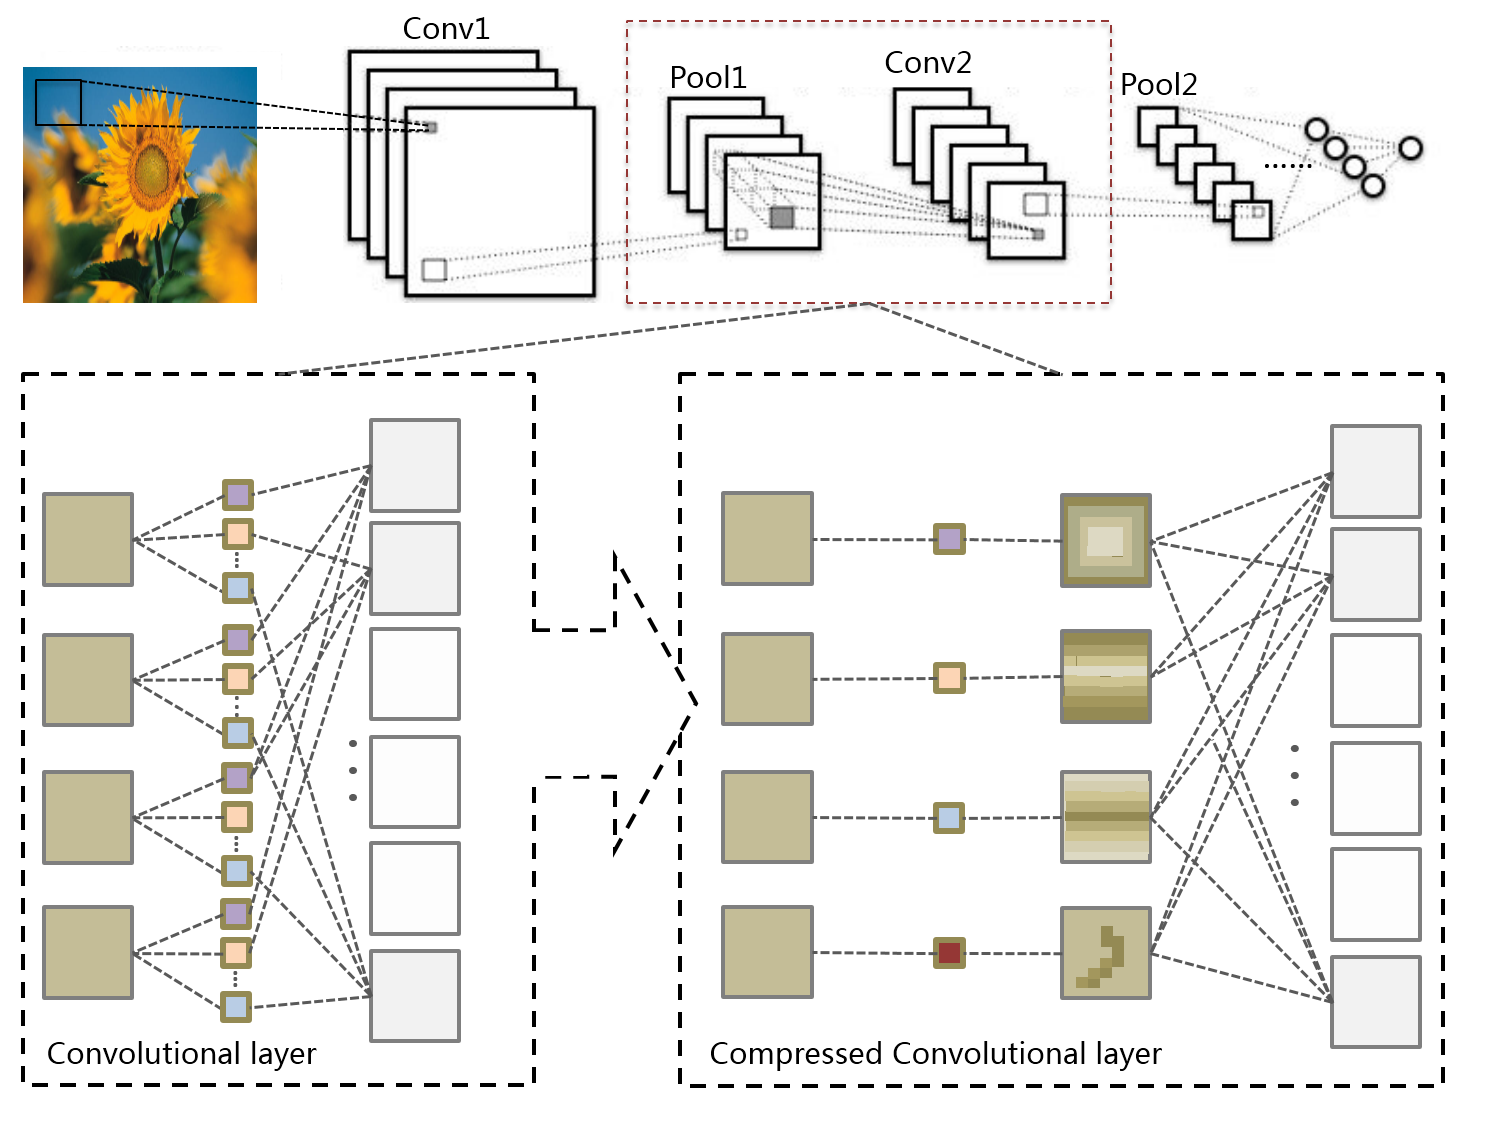
\includegraphics[width=1\columnwidth]{acc_old_intro.png}
\caption{主导卷积核参数压缩示意图。}
\label{fig:acc_old_intro}
\end{figure} 

受矩阵低秩分解~\cite{zhang2015efficient}启发,本章提出了一种新的基于主导卷积核(Dominant Convolutional Kernel,DK)分解的模型压缩方法,我们称之为DK分解。传统的卷积操作可以分解为两个步骤:特征提取和特征组合,在特征提取的过程中,通过挑选主导卷积核来缩减卷积参数,如图~\ref{fig:acc_old_intro}所示。模型压缩过程中,参数会大幅缩减,必然会引起网络性能的下降。受知识蒸馏~\cite{hinton2015distilling}思想启发,我们提出了知识预回归(Knowledge Pre-Regression,KP)的方法对压缩后的网络进行训练,尽量弥补网络因压缩所引起的精度损失。知识预回归是对FitNet~\cite{romero2014fitnets}训练方法的一种改进,采用全连接和交叉熵(Cross Entropy)损失函数来加速网络的收敛。知识预回归的训练方法有效地填补了教师网络与学生网络隐层特征之间的语义鸿沟。

本章采用主导卷积核(DK)分解的方法对大规模的教师网络进行压缩,采用知识预回归(KP)方法来训练压缩后的学生网络。我们将DK分解,KP训练的网络记为DK$^2$PNet,此网络有效地结合了目前主流的两种网络压缩方法。我们在四个数据集CIFAR-10~\cite{krizhevsky2009learning}、CIFAR-100~\cite{krizhevsky2009learning}、MNIST~\cite{lecun1998gradient}和SVHN~\cite{netzer2011reading}上对DK$^2$PNet进行了测试,与最近发表的很多CNN模型相比,DK$^2$PNet采用少量的参数,既可达到与其他模型接近的物体识别能力。

\section{相关工作}
\label{sec:acc:relate}

据我们了解,卷积模型加速的方法主要分为三个流派,分别是:模型压缩、知识蒸馏和硬件相关的加速方法。

模型压缩通过逐层地压缩卷积神经网络的参数,来实现模型的压缩与网络的加速。这种类型的方法通常由两部分组成,首先提出一种可以减少网络计算量的压缩方法,之后针对提出的压缩方法设计一种优化求解过程。对于优化求解,最常用的是卷积参数回归和数据回归两种方法。卷积参数回归,通过回归的方法直接重构卷积核参数。数据回归,通过回归的方式重构网络隐层的输出响应\cite{zhang2015efficient}。事实上,在模型压缩这个流派,压缩的方法往往受到更多的关注,其中基于矩阵低秩分解的方法是研究的热点之一。1989年,LeCun等人~\cite{lecun1989optimal}最早通过移除网络中不重要的权值参数,来实现网络加速的目的。Denil等人~\cite{denil2013predicting}证明了深度网络模型通常存在严重的过参数化(Over-Parameterization)现象,因此可以采用网络中一小部分参数子集去预测其他的参数。Jaderberg~\cite{jaderberg2014speeding} 进一步采用矩阵的低秩分解方法对网络的卷积层进行加速。他们采用两个秩为1的列向量对卷积核进行分解,逼近原有的卷积核。与此同时,Denton等人~\cite{denton2014exploiting}做了类似的工作,但是他们仅仅验证了这种分解方法在卷积网络的前两层的有效性。Lebedev等人~\cite{lebedev2014speeding}对四维卷积核在四个维度上进行了低秩分解,进一步压缩了网络的参数。Zhang等人~\cite{zhang2015efficient}在特征通道维度对卷积进行了分解,不同于以往的回归方法,对线性卷积核或线性输出特征进行回归,Zhang等人对网络的非线性激活响应进行回归。Chen等人~\cite{chen2015compressing} 提出了HashedNets,用散列去掉网络中固有的冗余信息。2016年,Iandola等人~\cite{iandola2016squeezenet}将卷积层替换为squeeze层和expand层,替换 $3\time3$ 的卷积核为 $1\time1$ 的卷积核并减少通道数,从而提出了SqueezeNet。Xception~\cite{chollet2016xception}是谷歌继Inception v3提出的一种改进,采用深层的分组卷积来替换Inception卷积。2017年,Howard等人\cite{howard2017mobilenets}提出Mobilenets,使用深层可分离的卷积来构建轻量级的深层神经网络,应用于移动和嵌入式设备。

另一种加速网络测试与预测时间的方法是基于知识蒸馏~\cite{hinton2015distilling}的训练方法,这种方法旨在通过用一个具有高识别率的教师网络去训练一个轻量的学生网络。知识蒸馏的概念是Hinton等人~\cite{hinton2015distilling}首次提出的,用于加快网络的预测时间。知识蒸馏是一种新颖的训练方法,将一个具有较高识别率的卷积网络网络中的“知识”进行压缩,迁移到被训练的目标网络。实际上,相似的想法早在2006年即被Bucilu$\check{a}$等人提及过,在他们的重要论文~\cite{bucilu2006model}中,成功地将多个复杂模型压缩成一个小的快速模型,并且没有引起明显的精度损失。与知识蒸馏类似,Ba和Caruana~\cite{ba2014deep}提出一个基于教师与学生网络体系结构的训练模型,他们证明了一个浅层网络也可以从深层网络模型中,学习到复杂的非线性映射关系,取得与深度网络近似的识别精度。Romero~\cite{romero2014fitnets}等人在这项工作的基础上,设计并成功训练出一个很深很瘦的网络FitNet,他们将知识蒸馏的理论从Softmax层推广到隐层,采用卷积回归的方式,将知识从教室网络的hint层,迁移到学生网络的guided层,提出了基于hint/guided结构的训练方法。

除此之外,与硬件相关的优化方法也可以加速网络,减少网络的预测时间。Vanhoucke等人~\cite{vanhoucke2011improving} 在低成本的x86 CPU上做了很多的优化工作,用于加速大规模矩阵运算。Farabet等人~\cite{farabet2011large}设计了适用于卷积运算的大规模FPGA集群。Krizhevsky~\cite{krizhevsky2014one}提出了一种新的适用于多GPU并行训练的并行化方法。cuda-convnet~\cite{krizhevsky2012imagenet}和caffe~\cite{jia2014caffe},两个开源的卷积神经网络计算框架,都提供了有效的GPU加速实现。此外,基于傅里叶变换,Mathieu等人~\cite{mathieu2013fast}将卷积操作从时域转换到频域,使得卷积操作加快了接近两倍。

\section{模型}
\label{sec:acc:model}

本节我们提出了基于主导卷积核(Dominant Convolutional Kernel,DK)分解的卷积压缩方法,和基于知识预回归(Knowledge Pre-Regression,KP)的网络训练方法,最后对两种方法与其他类似网络加速方法进行了分析与对比。

\subsection{主导卷积核}
\label{sec:acc:model:dk}

\begin{figure}
\centering
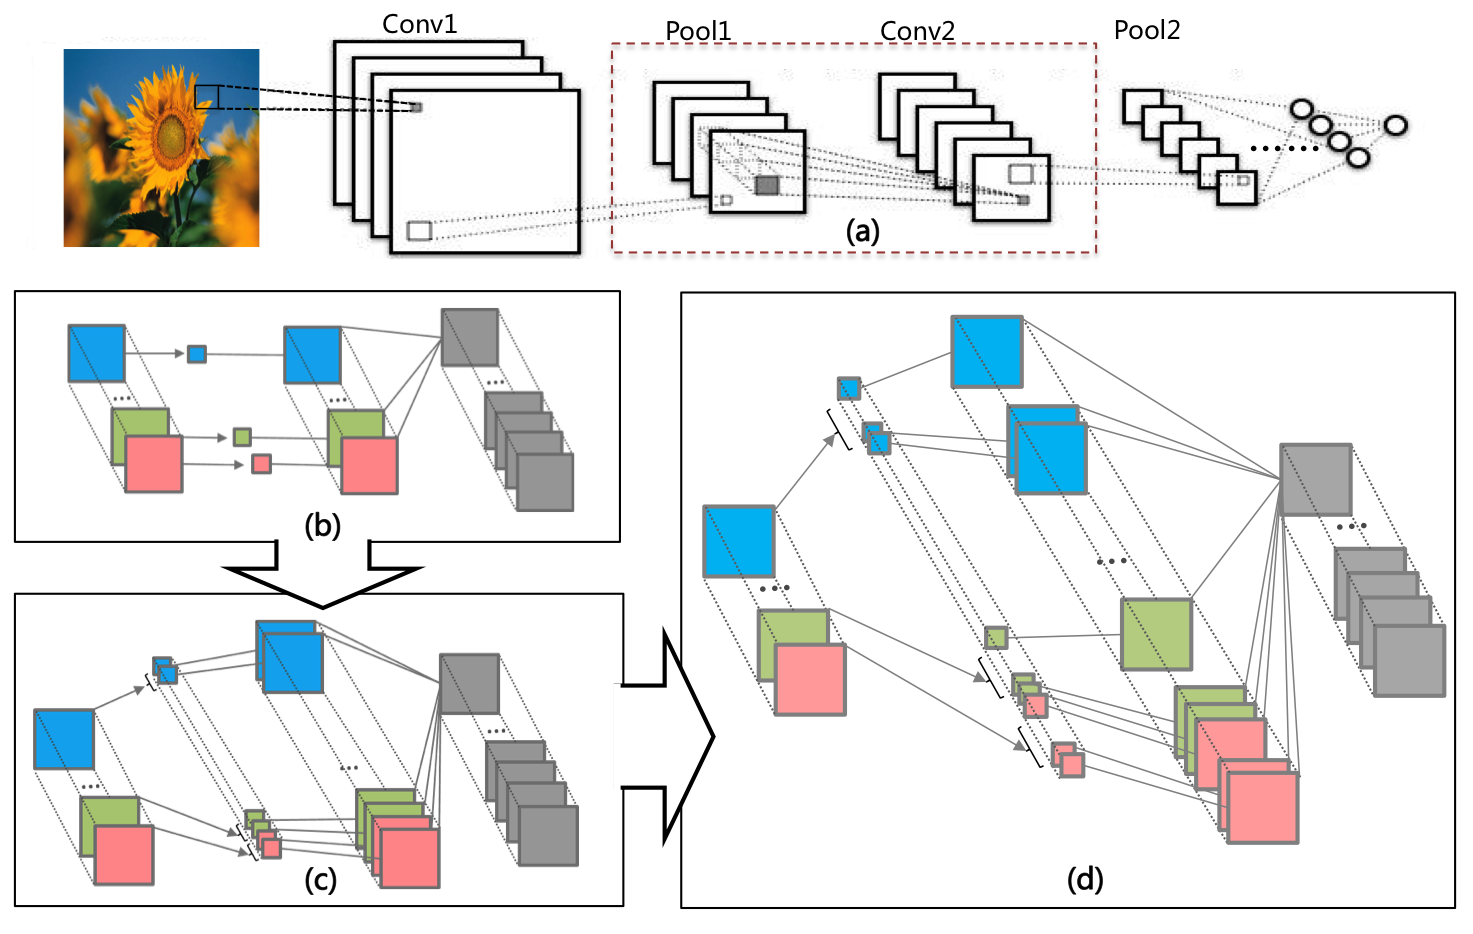
\includegraphics[width=1\columnwidth]{acc_dk.png}
\caption{主导卷积核。 (a) 传统卷积核;(b) 1比1情况下的主导卷积核;(c) 1比2情况下的主导卷积核;(d) 1比n情况下的主导卷积核。}
\label{fig:acc_dk}
\end{figure} 

在卷积神经网络中,具有大量参数的卷积操作对特征提取起到了至关重要的作用。实际上,大量的参数与计算量都集中在卷积层。因此对于卷积神经网络的压缩,最适合从卷积层参数压缩入手。因此,本节我们提出了基于主导卷积核分解的卷积参数压缩方法。

假设 $c_i$ 和 $c_o$ 分别代表卷积层输入和输出的通道数,$k_h$ 和 $k_w$ 分别代表卷积核的高度和宽度,对于传统的卷积方式,如图~\ref{fig:acc_dk} (a)所示,卷积核的大小为 $c_i{\times}c_o{\times}k_h{\times}k_w$。

卷积操作由乘法和加法运算组成,不同的卷积核与输入特征图的乘法操作可以理解为特征提取的过程,加法操作可以理解为特征组合的过程。将卷积操作理解为特征提取与特征组合,基于这样的观点,我们提出了主导卷积核分解,如图~\ref{fig:acc_dk} (b)(c)(d) 所示。以图~\ref{fig:acc_dk} (b)中1比1情况下的主导卷积核分解为例,对于每张输入特征图,我们只选择一个卷积核对其进行特征提取,再通过对所有特征进行线性加权的方式进行特征组合。特征提取可以通过分组卷积的方式实现,而特征选择可以通过使用具有 $1\times1$ 感受野大小的卷积操作实现。

对于传统的卷积方法如图~\ref{fig:acc_dk} (a)所示,每张输入特征图都和 $c_o$ 个卷积核进行卷积,对于图~\ref{fig:acc_dk} (b)中 1比1 情况下的主导卷积核,每个特征图只需要和一个卷积核进行卷积。上述过程可以推广到 1比2(如图~\ref{fig:acc_dk} (c)),1比$n$(如图~\ref{fig:acc_dk} (d))的情况,其中的 $n: 1{\le}n{\le}k_h{\times}k_w$ 称为主导卷积核的个数。在主导卷积核方法中,特征提取阶段的参数个数为 $n{\times}c_i{\times}k_h{\times}k_w$。在特征组合阶段,需要对所有特征提取阶段得到的中间结果进行线性加权,在特征选择阶段一共产生了$n{\times}c_i$ 组各不相同的特征,因此特征组合阶段需要的参数个数为 $n{\times}c_i{\times}c_o$。理论上说,当 $n$ 达到最大值 $k_h{\times}k_w$ 的时候,主导卷积核与传统的卷积等价。这是因为在线性代数理论中, $k_h{\times}k_w$ 个线性独立的特征向量构成了 $k_h{\times}k_w$ 维线性空间的一组基。

根据上述分析,主导卷积核分解的参数个数为  $n{\times}c_i{\times}k_h{\times}k_w+n{\times}c_i{\times}c_o$,是传统卷积参数个数的 $n/c_o+n/(k_h{\times}k_w)$ 倍。以一个常见的卷积层配置为例,对于一个具有 $3{\times}3$ 感受野大小,输入通道数为 96,输出通道数也为 96 的卷积层,主导卷积核仅需要 12\%(1比1情况)或 24\%(1比2情况)的参数规模。而卷积层的计算量与卷积层的参数个数是成正比的,因此采用主导卷积核对卷积层进行压缩,可以极大地提高网络的计算速度,减少运行时间。主导卷积核的个数 $n$ 可以用于平衡卷积层的特征提取能力和计算复杂度。

\subsection{知识预回归}
\label{sec:acc:model:kp}

\begin{figure}[t]
\centering
\centerline{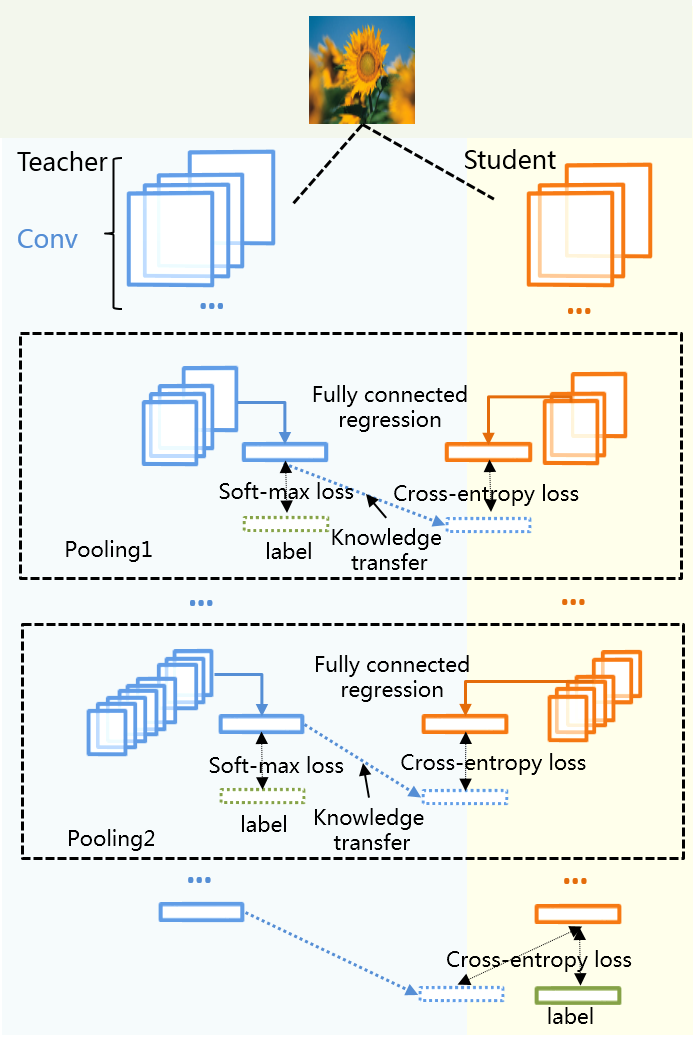
\includegraphics[height=1\columnwidth]{acc_old_kp.png}}
\caption{知识预回归。}
\label{fig:acc_kp}
\end{figure} 

知识蒸馏是2012年Hinton等人~\cite{hinton2015distilling}提出,用于将教师网络中的知识进行压缩,并迁移到学生网络的新型网络训练方法。网络的知识通常以网络参数的形式存储于卷积神经网络中,参数形式的知识太过于抽象以至于很难进行知识的迁移。Hinton等人将知识定义为一种从输入图像到目标类别概率(即Softmax层的输出)的非线性映射,知识迁移的最初的方式就是,将教师网络得到的概率分布迁移到学生网络。在第~\ref{sec:sam:vis}中可视化操作中,我们同样发现,哪怕对于错误的分类结果,卷积网络输出的概率分布仍然具有很大的参考价值。Romero等人~\cite{romero2014fitnets}将知识蒸馏的思想扩展到教师网络与学生网络的隐层,采用卷积回归的方式匹配隐层特征维度,再通过L2损失函数来回归对应隐层的激活响应。在此工作的基础上,本节提出了知识预回归方法对训练教师网络和学生网络进行知识回归。与Romero不同的是,我们在教师网络的隐层增加了一个额外的分类器,用于生成目标类别的概率分布,进一步采用交叉熵损失函数为优化目标,对学生网络的隐层特征进行回归,如图~\ref{fig:acc_kp}所示。实验结果表明,知识预回归相对于FitNet方法,更加稳定鲁棒,具有更快的收敛速度。

我们采用与~\cite{romero2014fitnets}相同的表述方式,即采用hint/guided对分别表示教师网络和学生网络对应的隐层对。通过DK分解对教师网络进行压缩,得到学生网路。因此,教师网络和学生网络具有相似的结构,但学生网络卷积层的特征拟合能力相对要若很多。采用逐层回归的方式对两个网络进行知识预回归往往难以起到较好的训练效果,根据我们的经验,选择对应的池化层作为hint/guided对进行知识预回归,可以有效地加快网络的收敛速度,提高学生网络的泛化能力。

选定的hint/guided对通常具有不同的特征维度,Romero等人~\cite{romero2014fitnets} 采用卷积回归来匹配特征维度,采用L2损失函数进行特征回归,这种方式虽然很简单,但是却很难收敛。我们采用知识预回归的方式来解决FitNet存在的不稳定和收敛慢等问题,如图~\ref{fig:acc_kp}所示。我们在 hint 层引入一个辅助分类器,该分类器由一个具有参数 $R_t$ 的全连接层,和一个 Softmax 层组成,采用图像真实的类别标签 $l$ 监督优化 $R_t$。该分类器的中间结果,会产生目标类别的概率分布 $b_t$,将此概率分布迁移到对应的guided层,来实现隐层知识的回归。类似地,对于学生网络,我们引入了另外一个辅助分类器,该分类器由一个以 $R_s$ 为参数的全连接层,和交叉熵函数组成。通过两个辅助分类器来建立hint层与guided层之间的联系,知识预回归的损失函数可以公式化表示为:
\begin{align} \label{equ:bridge}
\mathcal{L}_{KB}(W_s, R_t, R_s)={\lambda}\mathcal{H}(b_t^{\tau}, b_s^{\tau})+\mathcal{S}(l, b_t)
\end{align}
\begin{align} \label{equ:bt}
%b_t^{\tau}=\mathit{softmax}(\frac{{R_t}H_t}{\tau})
b_t^{\tau}=\mathit{softmax}(\frac{h(x; W_t, R_t)}{\tau})
\end{align}
\begin{align} \label{equ:bs}
%b_s^{\tau}=\mathit{softmax}(\frac{{R_s}G_s}{\tau})
b_s^{\tau}=\mathit{softmax}(\frac{g(x; W_s, R_s)}{\tau})
\end{align}
其中 $\mathcal{S}$ 和 $\mathcal{H}$ 分别代表 Softmax 和交叉熵损失函数;$h$ 和 $g$ 分别代表从输入图像 $x$ 到 hint 和 guided 层输出特征的非线性映射;$W_t$ 和 $W_s$ 分别指代教师网络和学生网络的参数;温度参数(Temperature Parameter)$\tau$~\cite{hinton2015distilling}用来弱化特征类别的概率分布;${\lambda}$ 用于调节两个损失函数的权重。

我们通过最小化下面这个公式来训练整个网络:
\begin{align} \label{equ:all}
%\mathcal{L}(W_s, R_t^{(1{\cdots}n)}, R_s^{(1{\cdots}n)})={\lambda}\mathcal{H}(p_t^{\tau}, p_s^{\tau}) + \mathcal{H}(l, p_s) + \sum_{i=1{\cdots}l}{\lambda}_i\mathcal{H}(b_t^{\tau^{(i)}}, b_s^{\tau^{(i)}})+\mathcal{S}(l, b_t^{(i)})
\mathcal{L}(W_s)={\lambda}\mathcal{H}(p_t^{\tau}, p_s^{\tau}) + \mathcal{S}(l, p_s) + \sum_{i=1{\cdots}P}{\lambda}_i\mathcal{H}(b_t^{\tau^{(i)}}, b_s^{\tau^{(i)}})+\mathcal{S}(l, b_t^{(i)})
\end{align}
其中 $p_t$ 和 $p_s$ 分别是教师网络和学生网络的目标类别概率分布;$P$ 代表我们选择的对应 hint/guided 层。在我们的实验中,我们选择了前两个池化层作为 hint/guided 层,用于知识预回归。

\subsection{分析与讨论}
\label{sec:acc:model:discuss}

\begin{figure}
\begin{center}
\centerline{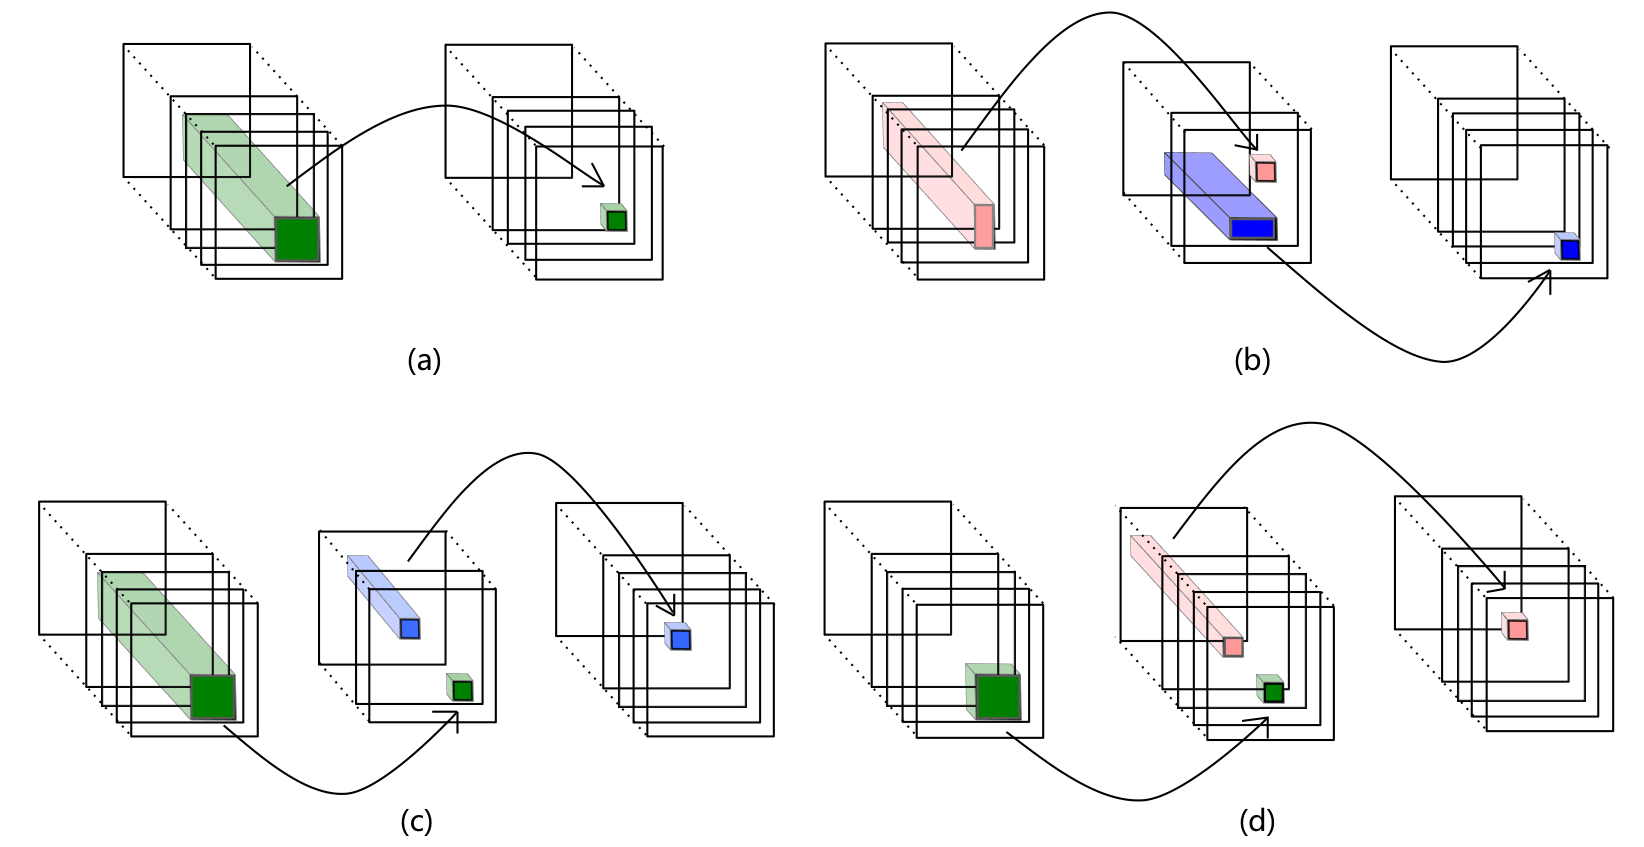
\includegraphics[width=1\linewidth]{acc_cmp.png}}
\caption{主导卷积核与其他压缩方法的对比。(a) 传统卷积操作;(b) Jaderberg~\cite{jaderberg2014speeding}的压缩方法;(c) Zhang~\cite{zhang2015efficient}的压缩方法;(d) 主导卷积核分解。}
\label{fig:acc_cmp}
\end{center}
\end{figure} 

第~\ref{sec:acc:model:dk}节中我们提出了基于主导卷积核分解的卷积分解方法,可以有效地压缩网络的参数,降低网络的计算量。尽管主导卷积核也是基于矩阵低秩分解的方法,但是与Jaderberg~\cite{jaderberg2014speeding}和Zhang~\cite{zhang2015efficient} 的方法不同,如图~\ref{fig:acc_cmp}所示。Jaderberg等人将传统的卷积操作分解为两次低秩线性映射,即对于原始的输入图像,分别采用具有 $1{\times}d$ 和 $d{\times}1$ 感受野大小的卷积核对其卷积参数进行分解。Zhang等人也采用两步分解,不同的是他们在通道上对卷积核进行了低秩分解。我们提出的主导卷积核如图~\ref{fig:acc_cmp}(d)所示,与Zhang等人的方法类似,也是在通道上对卷积核进行分解,与其不同的是,我们采用分组卷积的方式来降低特征维度,减少卷积参数与计算量。

为了加快被压缩网络的收敛速度,提高网络的泛化能力,我们提出了知识预回归的训练方法。在Hinton~\cite{hinton2015distilling}和Romero~\cite{romero2014fitnets}等人工作的基础上,我们对知识蒸馏和FitNet进行了拓展,如图\ref{fig:acc_kp}所示。知识预回归的训练结构看起来像两个并行的DSN~\cite{lee2015deeply}网络模型,但是他们具有不同的含义。DSN通过在隐层引入所谓的伴随优化目标来提高单个网络的特征表达能力,而知识预回归更多的关注于教师网络知识的压缩、提取与迁移。知识预回归方法使得学生网络可以学习到教师网络的特征表达能力与泛化能力。

\section{实验结果}
\label{sec:acc:experiment}

在开源项目caffe~\cite{jia2014caffe}基础上,我们对DK$^2$PNet网络进行了测试。所有的实验均运行于具有两颗GPU核心的单卡K80高性能服务器。在CIFAR-10~\cite{krizhevsky2009learning},CIFAR-100~\cite{krizhevsky2009learning},MNIST~\cite{lecun1998gradient}和 SVHN~\cite{netzer2011reading}四个数据集上,DK$^2$PNet均可以采用较少的模型参数与计算量达到一个较高的物体识别率。在CIFAR-10数据集上,我们进行了更多的实验来验证DK$^2$PNet方法的有效性。

在所有的实验中,我们均采用批大小(Batch Size)为96的批量随机梯度下降法来更新网络参数。网络的初始学习率设置为0.01,训练过程中当损失函数无法继续降低时对学习率进行调整,减小 10 倍,持续减小学习率三次,直到学习率减小到1e-5,所有卷积层偏执项的学习率均设为正常学习率的2倍。整个训练过程中,均采用 0.9 的动量因子(momentum)和 0.004 的权重衰减因子(weight decay)。在知识预回归的损失函数中(公式~\ref{equ:all}),参数$\lambda$,${\lambda}_1$ 和 ${\lambda}_2$的取值范围是[0.0001, 1],例如对于Softmax层 $\lambda=0.1$,第二个池化层 ${\lambda}_1=0.01$,第一个池化层 ${\lambda}_2=0.001$,即为一组有效的参数。对于每个数据集,我们均采用逐像素地减去训练样本像素均值的方式对图像进行预处理。

\subsection{网络结构}
\label{sec:acc:experiment:arc}

\begin{table}[t]
\begin{center}
\caption{基于主导卷积核分解的DK$^2$PNet-96网络识别性能对比。}
\label{tab:fit}
\begin{tabular}{L{5cm}C{2cm}C{3cm}}
 \toprule[1.5pt]
 {\heiti 模型} & {\heiti 参数个数} & {\heiti 测试错误率(\%)} \\
 \midrule[1pt]
 CNN-96 & 0.75 M & 7.82 \\
 \hline
 DK$^2$PNet-96(1比1,SGD)& 0.09 M & 9.59 \\
 DK$^2$PNet-96(1比2,SGD)& 0.18 M & 8.98 \\
 DK$^2$PNet-96(1比3,SGD)& 0.28 M & 8.55 \\
 DK$^2$PNet-96(1比4,SGD)& 0.37 M & 8.26 \\
 DK$^2$PNet-96(1比5,SGD)& 0.46 M & {\bf 7.98} \\
 DK$^2$PNet-96(1比6,SGD)& 0.55 M & 8.25 \\
 DK$^2$PNet-96(1比7,SGD)& 0.64 M & 8.56 \\
 DK$^2$PNet-96(1比8,SGD)& 0.73 M & 8.21 \\
 DK$^2$PNet-96(1比9,SGD)& 0.82 M & 8.03 \\
  \bottomrule[1.5pt]
\end{tabular}
\end{center}
\end{table}

本节中我们设计了一组结构相似但参数规模不同的网络。假设所有的卷积层,不论是传统卷积层还是主导卷积核卷积层,都具有相同的输入输出特征通道数 $K$,方便意见,采用与~\cite{liang2015recurrent}相同的符号表示,即CNN-$K$ 或者 DK$^2$PNet-$K$ 。其中CNN-$K$是教师网络,采用传统的卷积层,每个卷积层都具有 $K$ 个特征通道;DK$^2$PNet-$K$ 与 CNN-$K$ 结构类似,但是将其中的传统卷积层替换为主导卷积核卷积层,并采用知识预回归的方法进行网络训练。

教师网络CNN-$K$是一个具有 11 层结构的卷积网络模型,包括 10 个卷积层和 1 个全连接层。在网络的第 2 层、第 6 层和第 10 层之后,各接了一个池化层。最后采用Softmax层生成网络的目标概率。

学生网络DK$^2$PNet-$K$是对教师网络CNN-$K$进行主导卷积核分解得到的,具有与教师网络相类似的结构。对于第一个卷积层,输入图片最多具有3个通道,采用主导卷积核分解对该层压缩程度有限,因此对于第一个卷积层,并不对其进行压缩。对于CNN-$K$的第二到最有一个卷积层,采用主导卷积层替换传统卷积层,即得到DK$^2$PNet-$K$。

对于所有的卷积层,不论是传统卷积还是主导卷积,均采用 $3\times3$ 大小的感受野和 1 个像素的边界扩充和卷积滑动步长,这样可以保证输出和输入特征图具有相同的维度。对于前两个池化层,我们采用具有 $2\times2$ 感受野大小,步长为 2 的均值池化;最后一个池化层是全局均值池化。此外,所有的卷积层之后都采用BN层对卷积输出进行批正则化,采用ReLU作为非线性激活函数,采用Dropout来防止网络多拟合。对于DK2PNet-$K$(1比1)学生网络,一共具有 $(9K^2+108K)$ 个参数,而教师网络CNN-$K$的参数个数为$(81K^2+27K)$。


\subsection{CIFAR-10}
\label{sec:acc:experiment:cifar10}

CIFAR-10~\cite{krizhevsky2009learning}是Krizhevsky搜集并标注的一个图像识别数据集,具有 60,000 张 $32\times32$ 的彩色图片。

\begin{table} [t]
\begin{center}
\caption{知识预回归与梯度下降性能对比。}
\label{tab:kp}
\begin{tabular}{L{5cm}C{2cm}C{3cm}}
 \toprule[1.5pt]
 {\heiti 模型} & {\heiti 参数个数} & {\heiti 测试错误率(\%)} \\
 \midrule[1pt]
\multicolumn{3}{c}{\heiti 随机梯度下降} \\
\hline
DK$^2$PNet-96 (1比1, BN) & 0.09 M & {9.59} \\
DK$^2$PNet-96 (1比2, BN) & 0.18 M & {8.98} \\
DK$^2$PNet-128 (1比2, BN) & 0.32 M & {8.31} \\
DK$^2$PNet-160 (1比2, BN) & 0.49 M & {7.91} \\
 \midrule[1pt]
\multicolumn{3}{c}{\heiti 知识预回归} \\
\hline
高性能教师网络 & 0.75 M & 7.82 \\
DK$^2$PNet-96 (1比1, BN) & 0.09 M & {9.52} \\
DK$^2$PNet-96 (1比2, BN) & 0.18 M & {8.73} \\
DK$^2$PNet-128 (1比2, BN) & 0.32 M & {7.90} \\
DK$^2$PNet-160 (1比2, BN) & 0.49 M & {7.60} \\
\hline
低性能教师网络 & 0.75 M & 12.18 \\
DK$^2$PNet-96 (1比1, BN) & 0.09 M & {9.57} \\
DK$^2$PNet-96 (1比2, BN) & 0.18 M & {8.78} \\
DK$^2$PNet-128 (1比2, BN) & 0.32 M & {7.96} \\
DK$^2$PNet-160 (1比2, BN) & 0.49 M & {7.70} \\
  \bottomrule[1.5pt]
\end{tabular}
\end{center}
\end{table}

首先,我们通过一组对比实验来测试第~\ref{sec:acc:model:dk}节中主导卷积核分解对网络识别能力的影响,如表~\ref{tab:fit} 所示。其中网络CNN-96是本组对比实验的基准网络,该网络也是后文中将要用到的教师网络,具有不同压缩比的DK$^2$PNet-96作为对比研究对象。我们对九组DK$^2$PNet-96进行了测试,为了对比的公平,所有十个网络模型采用梯度下降算法进行训练,而没有引入知识预回归的训练策略,这里我们将采用梯度下降方法训练的DK$^2$PNet-96记为DK$^2$PNet-96(SGD)。实验结果如表~\ref{tab:fit} 所示,其中具有1比1压缩比的DK$^2$PNet-96仅仅采用 0.09M 参数,即达到了 9.59\% 的测试错误率,这有可能是CIFAR-10上测试误差低于 10\% 的最小模型。通过增大主导卷积核的个数降低压缩比,DK$^2$PNet-96 的识别率会逐渐提高,最好的压缩比率是1比5,此时 DK$^2$PNet-96 取得了 7.98\% 的测试错误率。意外的是,理论上与 CNN-96 等价,参数数量比 CNN-96 还要多的具有1比9压缩比的DK$^2$PNet-96,识别能力反而不如 CNN-96,我们猜测这可能是由网络参数冗余而产生的过拟合问题,影响了网络的泛化能力。


更进一步,我们设计了另外一组实验来验证第~\ref{sec:acc:model:kp}节中,知识预回归对网络性能的提升。我们将知识预回归方法与批量随机梯度下降方法进行了对比,实验结果如表~\ref{tab:kp} 所示。表~\ref{tab:kp} 中,四个具有不同压缩比和参数规模的DK$^2$PNet网络分别采用梯度下降法和知识预回归法进行训练。对于知识预回归训练方法,我们选取了测试误差率为 7.82\% 和 12.18\% 的两个教师网络分别训练学生网络。实验结果表明,在四组对比模型上,采用知识预回归的方法训练出的网络在最终的识别能力上都强于随机梯度下降的训练结果。对于具有1比1压缩比的DK$^2$PNet,知识预回归训练对其精度的提升非常有限,这是因为网络参数规模太小,网络的识别能力和泛化能力很难进一步提升。当测试网络的参数逐渐增加时,知识预回归对网络性能提升的幅度也会提高。此外我们还发现,相比于随机梯度下降法,即使我们用一个相对识别率较低的教师网络去训练学生网络,学生网络的识别率也是会受到影响的。当然,高性能的教师网络对学生网络的帮助更大。

\begin{table} [t]
\caption{正则化方法对DK$^2$PNet网络性能的影响。}
\label{tab:norm}
\begin{center}
\begin{tabular}{L{5cm}C{2cm}C{3cm}}
 \toprule[1.5pt]
 {\heiti 模型} & {\heiti 参数个数} & {\heiti 测试错误率(\%)} \\
 \midrule[1pt]
CNN-96 (LRN) & 0.75 M & 12.18 \\
DK$^2$PNet-96 (1比1, LRN) & 0.09 M & 26.88 \\
DK$^2$PNet-96 (1比2, LRN) & 0.18 M & 26.52 \\
DK$^2$PNet-128 (1比2, LRN) & 0.32 M & 25.01 \\
\hline
CNN-96 (BN) & 0.75 M & 7.82 \\
DK$^2$PNet-96 (1比1, BN) & 0.09 M & 9.59 \\
DK$^2$PNet-96 (1比2, BN) & 0.18 M & 8.98 \\
DK$^2$PNet-128 (1比2, BN) & 0.32 M & 8.31 \\
  \bottomrule[1.5pt]
\end{tabular}
\end{center}
\end{table}

正则化方法对网络的性能具有至关重要的影响,DK$^2$PNet可以在参数很少的情况下,取得如此卓越的识别能力,很大程度上要归功于批正则化(Batch Normalization,BN)~\cite{ioffe2015batch}方法。关于正则化对网络性能的影响,我们在CNN-96和DK$^2$PNet上进行了两组实验,一组采用批正则化方法,另一组采用局部响应正则化方法(Local Response Unit,LRN),对比结果如表~\ref{tab:norm} 所示。显然,批正则化方法的性能远远优于局部响应正则化方法,可见正则化方法对网络性能的提升起到了重要的作用。实际上,应用于池化层的知识预回归训练,在一定程度上也起到正则化的作用,通过回归的方式,强制学生网络的去学习教师网络的特征提取方式与泛化能力。

\begin{table} [!h]
\begin{center}
\caption{CIFAR-10数据集上与已知模型的对比试验。}
\label{tab:cifar10}
\begin{tabular}{L{5cm}C{2cm}C{3cm}}
 \toprule[1.5pt]
 {\heiti 模型} & {\heiti 参数个数} & {\heiti 测试错误率(\%)} \\
 \midrule[1pt]
\multicolumn{3}{c}{\heiti 没有数据增广} \\
\hline
\noalign{\smallskip}
Maxout~\cite{goodfellow2013maxout} & $>$5 M & 11.68 \\
Prob maxout~\cite{springenberg2013improving} & $>$5 M & 11.35 \\
NIN~\cite{lin2013network} & 0.97 M & 10.41 \\
DSN~\cite{lee2015deeply} & 0.97 M & 9.69 \\
RCNN~\cite{liang2015recurrent} & 1.86 M & 8.69 \\
ALL-CNN~\cite{springenberg2014striving} & 1.4 M & 9.08 \\
Tree+Max-Avg~\cite{lee2015generalizing} & 1.85M & 7.62 \\
DenseNet~\cite{huang2016densely} & 15.3M & \bf{5.19} \\
\hline
\noalign{\smallskip}
Teacher (CNN-96) & 0.75 M & 7.82 \\
DK$^2$PNet-96 (1比1) & 0.09 M & 9.52 \\
DK$^2$PNet-96 (1比2) & 0.18 M & 8.73 \\
DK$^2$PNet-128 (1比2) & 0.32 M & {7.90} \\
DK$^2$PNet-160 (1比2) & 0.49 M & \bf{7.60} \\
 \midrule[1pt]
\multicolumn{3}{c}{\heiti 具有数据增广} \\
\hline
Maxout~\cite{goodfellow2013maxout} & $>$5 M & 9.38 \\
dasNet~\cite{stollenga2014deep} &  $>$5 M & 9.22 \\
Prob maxout~\cite{springenberg2013improving} & $>$5 M & 9.39 \\
DropConnect~\cite{wan2013regularization} & - & 9.32 \\
NIN~\cite{lin2013network} & 0.97 M & 8.81 \\
DSN~\cite{lee2015deeply} & 0.97 M & 8.22 \\
RCNN~\cite{liang2015recurrent} & 1.86 M & 7.09 \\
Highway Network~\cite{srivastava2015training} & 2.3 M & 7.54 (7.72${\pm}$0.16) \\
ALL-CNN~\cite{springenberg2014striving} & 1.4 M & 7.25 \\
ResNet~\cite{he2015deep} & 1.7M & {6.43 (6.61${\pm}$0.16)} \\
Fitnet4-LSUV~\cite{mishkin2015all} & 2.5M & 6.06 \\
Tree+Max-Avg~\cite{lee2015generalizing} & 1.85M & 6.05 \\
Tuned CNN~\cite{snoek2015scalable} & 1.29M & 6.37 \\
DenseNet~\cite{huang2016densely} & 25.6M & \bf{3.46} \\
\hline
DK$^2$PNet-96 (1比1) & 0.09 M & {8.78} \\
DK$^2$PNet-96 (1比2) & 0.18 M &{7.68} \\
DK$^2$PNet-128 (1比2) & 0.32 M & 7.06 \\
DK$^2$PNet-160 (1比2) & 0.49 M & 7.06 \\
DK$^2$PNet-256 (1比1) & 0.62 M & \bf{6.44} \\
  \bottomrule[1.5pt]
%\multicolumn{3}{c}{{\bf{Extreme}} Data Augmentation} \\
%\hline
%Large ALL-CNN~\cite{springenberg2014striving} & - & 4.41 \\
%Fractional MP~\cite{graham2014fractional} & - & 3.47 \\
%\hline
\end{tabular}
\end{center}
\end{table}

最后,在没有数据増广的情况下,我们对DK$^2$PNet与其他优秀模型进行了实验对比。首先,我们训练了一个具有 0.75M 参数的教师网络CNN-96,此教师网络的测试错误率为7.82\%。之后,我们采用主导卷积核分解的方法对CNN-96进行压缩,得到1比2情况下的学生网络DK$^2$PNet-96,并采用知识预回归的方法对学生网络进行训练,实验结果如表~\ref{tab:cifar10},DK$^2$PNet-96(1比2)在只有 0.19M 参数的情况下,取得了8.73\%的测试错误率。之后,我们对DK$^2$PNet-96(1比2)进行了扩展,在每层加入了更多的隐层节点,得到的DK$^2$PNet-160(1比2)在0.49M参数规模的情况下,得到了 7.60\% 的测试错误率,此网络的性能甚至超过了教师网络。


此外,我们对CIFAR-10进行了具有平移和水平翻转的数据増广,并在此情况下对DK$^2$PNet进行了测试。在训练阶段,我们从原始训练图片中随机截取出一张 $24\times24$ 像素大小的图像,并随机地对其进行水平翻转。在测试阶段,对于每张测试图片截取十张 $24\times24$ 像素大小的测试样本进行测试,其中一半样本进行了水平翻转増广。具有 0.09M 参数的DK$^2$PNet-96(1比1)取得了 8.78\% 的测试错误率,DK$^2$PNet-256(1比1)仅仅采用 0.62M 的参数,即取得了与具有100层之深的ResNet~\cite{he2015deep}相当的测试错误率。

\subsection{CIFAR-100}
\label{sec:acc:experiment:cifar100}

CIFAR-100是一个与CIFAR-10类似的数据集,但是类别的数量扩展到了 100 类。采用与CIFAR-10类似的方法,我们在CIFAR-100数据集上训练了四个DK$^2$PNet网络模型,并与CIFAR-100上取得优秀结果的模型进行了对比,实验结果如表~\ref{tab:cifar100} 所示。从实验结果可以看出,DK$^2$PNet-160(1比2)在没有数据増广的情况下取得了 31.39\%的测试错误率,但是仅仅采用了 0.49M 的参数数量。DK$^2$PNet-160(1比2)取得了比RCNN~\cite{liang2015recurrent}更好的识别率,但是却仅仅采用了相对于RCNN 模型 26\% 的参数规模。

\begin{table} [t]
\caption{CIFAR-100数据集上与已知模型的对比试验。}
\label{tab:cifar100}
\begin{center}
\begin{tabular}{L{5cm}C{2cm}C{3cm}}
 \toprule[1.5pt]
 {\heiti 模型} & {\heiti 参数个数} & {\heiti 测试错误率(\%)} \\
 \midrule[1pt]
\multicolumn{3}{c}{\heiti 没有数据增广} \\
\hline
Maxout~\cite{goodfellow2013maxout} & $>$5 M & 38.57 \\
dasNet~\cite{stollenga2014deep} & $>$5 M & 33.78 \\
Prob maxout~\cite{springenberg2013improving} & $>$5 M & 38.14 \\
Tree based priors~\cite{srivastava2013discriminative} & - & 36.85 \\
NIN~\cite{lin2013network} & 0.98 M & 35.68 \\
DSN~\cite{lee2015deeply} & 0.98 M & 34.57 \\
RCNN~\cite{liang2015recurrent} & 1.86 M & \bf{31.75} \\
ALL-CNN~\cite{springenberg2014striving} & 1.3 M & 33.71 \\
Highway Network~\cite{srivastava2015training} & 2.3 M & 32.24 \\
Tree+Max-Avg~\cite{lee2015generalizing} & 1.76 M & 32.37 \\
ELU-Network~\cite{clevert2015fast} & 39.32 M & 24.28 \\
DenseNet~\cite{huang2016densely} & 15.3M & \bf{19.64} \\
\hline
Teacher (CNN-96) & 0.75 M & {33.63} \\
DK$^2$PNet-96 (1比1) & {0.09 M} & {38.51} \\
DK$^2$PNet-96 (1比2) & {0.18 M} & {35.24} \\
DK$^2$PNet-128 (1比2) & {0.32 M} & {34.48} \\
DK$^2$PNet-160 (1比2) & {0.49 M} & \bf{31.39} \\
\hline
\multicolumn{3}{c}{\heiti 具有有数据增广} \\
\hline
Fitnet4-LSUV~\cite{mishkin2015all} & 2.5 M & 27.66 \\
Tuned CNN~\cite{snoek2015scalable} & 1.29 M & 27.40 \\
DenseNet~\cite{huang2016densely} & 25.6M & \bf{17.18} \\
  \bottomrule[1.5pt]
%\multicolumn{3}{c}{{\bf{Extreme}} Data Augmentation} \\
%\hline
%Fractional MP~\cite{graham2014fractional} & - & 26.39 \\
%\hline
\end{tabular}
\end{center}
\end{table}

主导卷积核分解是受矩阵低秩分解启发所提出的一种有效的卷积参数压缩方式。主要思想源于将传统的卷积操作分解为两步操作:特征提取和特征组合,在特征提取的过程中,通过挑选主导卷积核来缩减卷积参数。主导卷积核分解可以极大地压缩卷积神经网络模型中卷积层参数。而不同的主导卷积核个数,决定了模型参数压缩的比率。在CIFAR-100数据集上,如表~\ref{tab:cifar100}所示,我们设计的网络在参数规模上远远少于其他网络模型结构。但是模型参数的压缩,必然会因此网络识别能力的下降。为了尽量弥补模型因参数压缩所带来的识别精度损失问题,我们提出了知识预回归的网络训练方式,采用全连接和交叉熵(Cross Entropy)损失函数来加速网络的收敛。知识预回归的训练方法有效地填补了教师网络(原网络)与压缩后的学生网络隐层特征之间的语义鸿沟。

此外,在CIFAR-100数据集的实验中,我们还给出了一种模型调优的有效方法。如表~\ref{tab:cifar100}所示,我们选用的教师网络具有 0.75M 的网络参数和 33.63\%的测试错误率,采用本章提出的主导卷积核分解和知识预回归的方式,我们首先对教师网络进行了模型压缩与加速,分别训练出了DK$^2$PNet-96(1比1)和DK$^2$PNet-96(1比2)两个分别具有 0.09M 和 0.18M 参数规模的快速学生网络,但是这两个模型的识别能力却低于教师网络。在DK$^2$PNet-96(1比2)的基础上,我们对模型进行加宽,增加模型的参数与识别能力,分别得到了DK$^2$PNet-128(1比2)和DK$^2$PNet-160(1比2)。随着网络的加宽和参数数量的提升,网络的识别性能也在逐步提升,当网络加宽到DK$^2$PNet-160(1比2)时,该模型的测试错误率已经达到31.39\%,识别能力超过了教师网络,而模型的参数却仅仅是0.49M,还要低于教师网络的0.75M。由此可见,将繁重的大模型压缩为规模较小的快速模型,之后对该模型进行复用甚至加宽加深,来设计并训练出性能和预测速度均超越教师网络的快速模型,是一种十分有效的模型调优方法。


\subsection{MNIST}
\label{sec:acc:experiment:mnist}

\begin{table} [h]
\caption{MNIST数据集上与已知模型的对比试验。}
\label{tab:mnist}
\begin{center}
\begin{tabular}{L{5cm}C{2cm}C{3cm}}
 \toprule[1.5pt]
 {\heiti 模型} & {\heiti 参数个数} & {\heiti 测试错误率(\%)} \\
 \midrule[1pt]
\multicolumn{3}{c}{\heiti 没有数据增广} \\
\hline
Maxout~\cite{goodfellow2013maxout} & 0.42 M & 0.45 \\
NIN~\cite{lin2013network} & 0.35 M & 0.47 \\
DSN~\cite{lee2015deeply} & 0.35 M & 0.39 \\
RCNN~\cite{liang2015recurrent} & 0.67 M & 0.31 \\
Tree+Max-Avg~\cite{lee2015generalizing} & 1.85 M & 0.31 \\
FitNet-LSUV-SVM~\cite{mishkin2015all} & 0.03 M & 0.38 \\
Tree+Max+Avg~\cite{lee2015generalizing} & 1.85 M & \bf{0.29} \\
\hline
Teacher (CNN-64) & 0.33 M & {0.33} \\
%DK$^2$PNet-64 (1比1, KB) & {0.04 M} & {0.38} \\
DK$^2$PNet-64 (1比2) & {0.09 M} & {0.38} \\
DK$^2$PNet-96 (1比1) & {0.09 M} & {0.36} \\
DK$^2$PNet-96 (1比2) & {0.18 M} & \bf{0.31} \\
\hline
\multicolumn{3}{c}{\heiti 具有数据增广} \\
\hline
Dropconnect~\cite{wan2013regularization} & - & 0.21 \\
MCDNN\cite{ciresan2012multi} & - & 0.23 \\
  \bottomrule[1.5pt]
\end{tabular}
\end{center}
\end{table}

MNIST~\cite{lecun1998gradient} 是一个阿拉伯数字 0 到 9 的数字手写体识别数据集,其中的图片是 $28{\times}28$ 像素大小的灰度图。因为这个数据集相对比较简单,相对较小规模的网络即可达到一个较好的识别率。从表~\ref{tab:mnist}的实验结果可以看出,DK$^2$PNet-96(1比2)取得了与RCNN~\cite{liang2015recurrent}和Tree+Max-Avg~\cite{lee2015generalizing}相同的测试错误率0.31\%,但是DK$^2$PNet-96(1比2)使用的参数仅仅是RCNN的29\%,Tree+Max-Avg的10\%。

\subsection{SVHN}
\label{sec:acc:experiment:svhn}

\begin{table} [h]
\caption{SVHN数据集上与已知模型的对比试验。}
\label{tab:svhn}
\begin{center}
\begin{tabular}{L{5cm}C{2cm}C{3cm}}
 \toprule[1.5pt]
 {\heiti 模型} & {\heiti 参数个数} & {\heiti 测试错误率(\%)} \\
 \midrule[1pt]
Maxout~\cite{goodfellow2013maxout} & $>$5 M & 2.47 \\
Prob maxout~\cite{springenberg2013improving} & $>$5 M & 2.39 \\
NIN~\cite{lin2013network} & 1.98 M & 2.35 \\
DSN~\cite{lee2015deeply} & 1.98 M & 1.92 \\
RCNN~\cite{liang2015recurrent} & 2.67 M & 1.77 \\
Tree+Max+Avg~\cite{lee2015generalizing} & 4.00M & 1.69 \\
DenseNet~\cite{huang2016densely} & 27.2M & \bf{1.59} \\
\hline
Teacher (CNN-96) & 0.75 M & {1.82} \\
%DK$^2$PNet-96 (1比1, KB) & {0.09 M} & {2.17} \\
DK$^2$PNet-96 (1比2) & {0.18 M} & {2.04} \\
DK$^2$PNet-128 (1比2) & {0.32 M} & {1.95} \\
DK$^2$PNet-160 (1比2) & {0.49 M} & \bf{1.83} \\
  \bottomrule[1.5pt]
\end{tabular}
\end{center}
\end{table}


SVHN~\cite{netzer2011reading}也是一个数字识别的数据集,但是其中的图片采集自谷歌街景地图。因为图片来自真实环境,光照和清晰度变化剧烈,因此识别难度较高。表~\ref{tab:svhn}中的实验结果表明,具有0.49M 参数的DK$^2$PNet-160 (1比2) 即可以取得1.83\%的测试错误率,相对于近期提出的RCNN~\cite{liang2015recurrent},Tree+Max+Avg~\cite{lee2015generalizing}和DenseNet~\cite{huang2016densely},大大缩减了网络的参数。

\section{本章小结}
\label{sec:acc:conclusion}

本章我们提出了一种基于主导卷积核分解和知识预回归的网路压缩方法。首先,通过主导卷积核分解对卷积参数进行压缩。再通过知识预回归的训练方法,将教师网络隐层的知识进行压缩并迁移到学生网络,指导学生网络去学习教师网络的特征提取方式与泛化能力,尽量弥补由网络压缩所造成的精度损失。知识预回归可以有效地加速学生网络的收敛,提高学生网络的特征拟合能力与泛化能力。最后,在CIFAR-10、CIFAR-100、MNIST和SVHN四个数据集上,我们对DK$^2$PNet进行了测试。实验结果表明,DK$^2$PNet在四个数据集上均取得了与最好结果相近的识别率,但却大大缩减了网络的参数和测试时间。


\chapter{基于卷积神经网络的交通标志识别}
\label{cha:seg}

\section{引言}
\label{sec:seg:introduction}

交通标志识别是无人驾驶汽车(Unmanned Ground Vehicle,UGV)和高级辅助驾驶(Advanced Driver Assistance Systems,ADAS)技术的一个重要组成部分。在驾驶行为中,驾驶员的大部分精力主要集中在结构化的道路结构和前方车辆,很容易忽视路旁小尺寸的交通标志。智能的交通标志检测可以有效地避免不必要的违章甚至交通事故。传统的计算机视觉算法曾被广泛地应用于交通标志识别任务中~\cite{le2010real},近年来卷积神经网络模型和算法的改进与完善,使得卷积神经网络在物体识别任务上取得了重大的突破。得益于计算机计算能力的提高,尤其是GPU并行计算能力的提升,使我们可以采用卷积神经网络方法去解决交通标志识别的问题。

交通标志识别并不是一个很简单任务,交通标志图像具有不同的视角、遮挡、模糊程度和尺寸变化。真实世界的环境因素也会对拍摄到的交通标志产生影响,在不同的车速、光照和天气条件下,采集到的图像会有很大的区别。此外,交通标志牌的褪色和磨损,不同时期布置的交通标志牌之间的差异等因素,都会给识别任务带来极大的困难与挑战。本章的实验对象为德国交通标志数据集(German Traffic Sign Recognition Benchmark,GTSRB)~\cite{stallkamp2012man},此数据集中的图片如图~\ref{fig:tsr_data}所示。图~\ref{fig:tsr_data}(a)列举了一些不同种类的训练交通标志样本,图~\ref{fig:tsr_data}(b)是部分不同环境因素下测试交通标志样本。德国的交通标志与大部分欧洲国家、印度和中国等国家的交通标志非常相似,是一个用于研究交通标志识别很好的公开数据集。

\begin{figure*}[t]
\centering
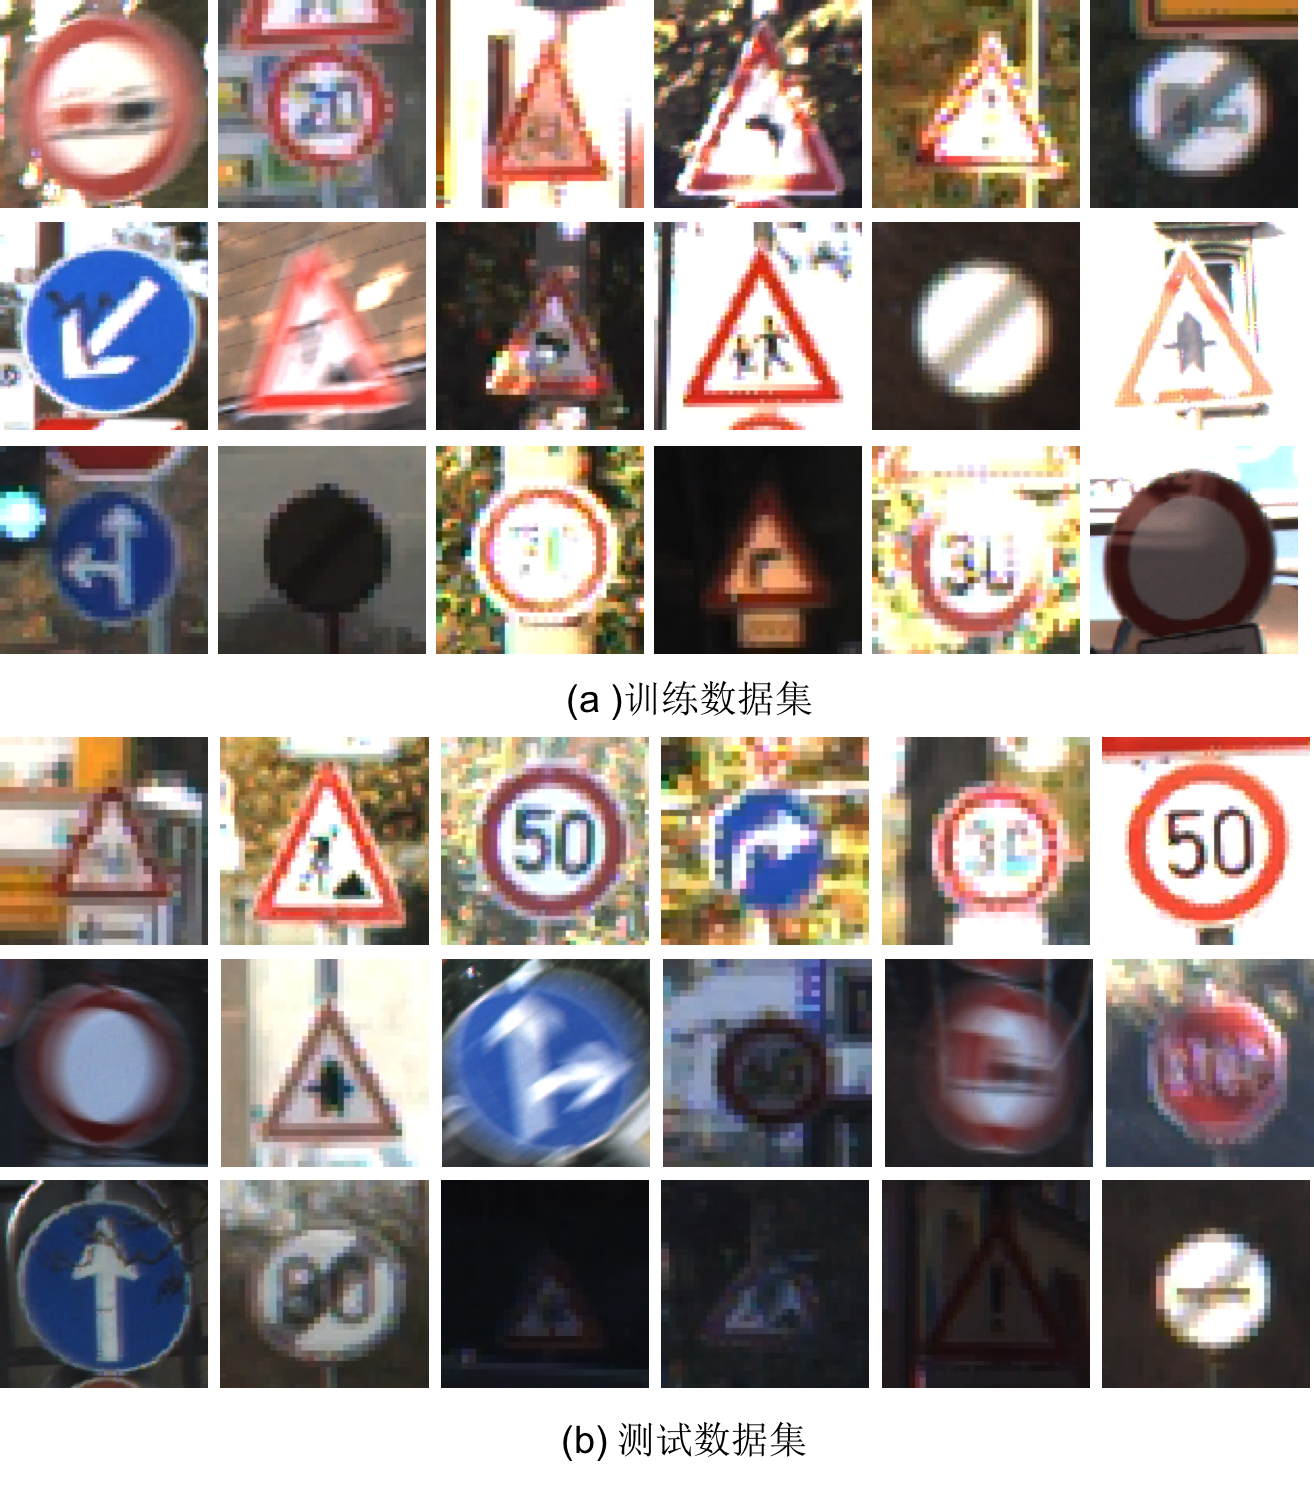
\includegraphics[width=0.9\linewidth]{tsr_train_test.png}
\caption{GTSRB图像样本。图中(a)是一些不同种类的训练交通标志样本,(b)是部分不同环境因素下测试交通标志样本。交通标志图像具有不同的视角、遮挡、模糊程度和尺寸变化。真实世界的环境因素也会对拍摄到的交通标志产生影响,在不同的车速、光照和天气条件下,采集到的图像会有很大的区别。此外,交通标志牌的褪色和磨损,不同时期布置的交通标志牌之间的差异等因素,都会给识别任务带来极大的困难与挑战。}
\label{fig:tsr_data}
\end{figure*}


本章我们以交通标志识别为应用背景,对论文第二、三、四章提出的方法进行了验证、对比与分析。第二章我们对卷积神经网络的卷积层进行改进,提出了一种组合卷积卷积结构:自适应卷积层(SAM),来简化复杂卷积神经网络的设计过程。SAM结构以Inception~\cite{szegedy2014going,szegedy2015rethinking,szegedy2016inception}为基础框架,结合了最大输出单元(Maxout)~\cite{goodfellow2013maxout},残差网络(ResNet)~\cite{he2015deep}和网络中的网络(NIN)~\cite{DBLP:journals/corr/LinCY13}四个模型的优势,可以有效地简化复杂深层网络的设计过程。第三章我们对卷积神经网络的池化层进行改进,提出了随机区域池化方法(SAP)来实现特征层的数据増广。SAP通过对池化区域进行随机的仿射变换,对特征进行重采样,在不影响特征空间样本分布的情况下对特征进行扰动,增加特征的多样性,最终实现特征増广,可以有效地提高网络的泛化能力。第四章我们提出了一种卷积神经网络模型压缩与加速方法,先通过主导卷积核分解对卷积层进行参数压缩与网络加速,再通过知识预回归的训练方法来尽量弥补压缩造成的精度损失。本章针对交通标志识别任务,对第二章和第三章的网络模型进行了测试与对比,并将两种方法进行结合,最后采用第四章的方法对模型进行加速,加快网络的推理速度,减少网络预测时间。本章其余内容组织如下:第~\ref{sec:seg:relate}节简要回顾了交通标志识别的相关研究工作;第\ref{sec:seg:model}节详细介绍了如何将组合卷积结构、随机区域池化和网络加速方法共同应用于交通标志识别任务;第~\ref{sec:seg:exp}节对实验结果进行了分析与讨论;第~\ref{sec:seg:conclusion}是对本章主要内容的总结。

\section{相关工作}
\label{sec:seg:relate}

交通标志的检测与识别是无人驾驶汽车和高级辅助驾驶技术中的一个重要研究课题。很多传统的机器学习方法致力于解决真实环境中由于尺寸、视角和清晰度的不同所产生的识别难题。2005年,Bahlmann等人~\cite{bahlmann2005system}综合考虑颜色、形状和运动信息,采用哈尔小波特征进行交通标志的检测、跟踪与识别。该方法具有较大的计算量,并且识别精度较低,虽然综合了交通标志颜色、形状和相机运动等信息,但是没有考虑到图像上下文的信息。2010年,Le等人~\cite{le2010real}采用支持向量机(SVM)对视频流中的颜色块进行检测,检索出交通标志可能出现的区域。Le等人重点研究了不同天气情况对交通标示识别的影响,但是该方法仅仅考虑了交通标志的颜色信息,且计算量较大。2011年,Zaklouta等人~\cite{zaklouta2011traffic}分别采用KD树和随机森林的方法对交通标志进行识别,论文还对比了不同尺度的HOG特征和距离变换函数对交通标志识别的影响。实验结果表明随机森林结合细粒度的HOG特征可以取得较好的识别率,但是Zaklouta等人并没有在论文中考虑交通标志的颜色信息。2012年,Lu等人~\cite{lu2012sparse}提出了一种基于稀疏编码的交通标志识别方法。2015年,Haloi等人~\cite{haloi2015novel}提出了一种基于概率潜在语义分析模型(Probabilistic Latent Semantic Analysis,pLSA)的交通标志识别系统,该系统采用由SIFT特征构成的词袋模型对图像的形状和交通标志的类别分别进行识别。Haloi等人的方法具有较快的识别速度,但是该方法也没有考虑交通标志的颜色和图像上下文信息。


基于卷积神经网络的识别方法在交通标志识别任务中取得了更好的识别率,2011年,Sermanet等人~\cite{sermanet2011traffic}在2011年的GTSRB交通标示识别竞赛中,采用具有两层结构的多尺度卷积神经网络逐层地学习特征,取得了98.97\%的识别率,超过了人类98.84\%~\cite{stallkamp2011german}的识别水平。之后,Sermanet等人进一步增加网络的参数规模,忽略图像的颜色信息,采用灰度图对网络进行训练和测试,在GTSRB数据集上取得了99.17\%的识别率。Sermanet等人采用的卷积网络只有两层的深度,没有充分挖掘出深层网络在特征提取方面的能力,两层网络所具有的感受野无法充分的提取图像的上下文信息。同年,Cirecsan等人~\cite{cirecsan2011committee}训练了25个具有三个卷积层和两个全连接层的卷积神经网络,并对输入图像进行了数据増广,采用多模型平均的方式,在GTSRB数据集上取得了99.46\%的识别率。该方法的主要缺点在于需要训练多个卷积神经网络模型,消耗大量的参数与计算量。2015年,Haloi~\cite{haloi2015traffic}等人结合空间变换网络~\cite{jaderberg2015spatial}和改进的Inception~\cite{szegedy2014going,szegedy2015rethinking,szegedy2016inception}结构,来提取具有平移、旋转和缩放不变性的特征,在GTSRB数据集上取得了99.81\%的识别率。该方法在GTSRB数据集上取得了最高的识别率,但是网络参数过多,计算量加大,很难应用于实际场景。2016年,Zhu等人~\cite{zhu2016traffic}联合腾讯地图发布了一个交通标示检测与识别的数据集清华-腾讯100K,该数据集图像主要来自腾讯街景地图。此外Zhu等人提出了一个端到端的交通标志检测与识别卷积神经网络模型,该网络可以同时解决检测与识别问题。

\section{交通标志识别}
\label{sec:seg:model}

第二章我们提出了卷积层的一种改进方法组合卷积结构,第三章我们提出了池化层的一种改进方法随机区域池化,第四章我们提出了一种基于主导卷积核和知识预回归的网络模型压缩与网络加速方法。这三章内容可以有效地组合,用于视觉物体的识别任务。组合卷积结构和随机区域池化可以提高网络的识别率,主导卷积核通过对卷积层进行低秩分解来减少网络的参数与计算量,再通过知识预回归的训练方式来弥补由于模型压缩所产生的精度损失。本小结中,我们首先结合组合卷积结构和随机区域池化层,提出了一个具有特征增广的自适应卷积网络模型(Self-adaptive Network with Feature Augmentation,FASNet)。此外,为了压缩模型的参数规模,加快网络的预测时间,我们采用主导卷积核分解对FASNet进行压缩与加速。


\begin{table}[h]
\caption{FASNet网络结构。}

\label{tab:fas}
\centering
\begin{tabular}{ccccccc}
 \toprule[1.5pt]
%{\heiti 类型} & {\heiti 感受野/步长} & {\heiti 输出特征维度} & {\heiti 分支1} & {\heiti 分支2} & {\heiti 选择器} & {\heiti 参数} \\
\multirow{2}{*}{\heiti 类型} & \multirow{2}{*}{\heiti 感受野/步长} & \multirow{2}{*}{\heiti 输出特征维度} & \multicolumn{3} {c}{SAM结构} &  \multirow{2}{*}{\heiti 参数} \\
\cline{4-6} &&&  {\heiti 分支1} & {\heiti 分支2} & {\heiti 选择器} \\
\midrule[1pt]
卷积层 & 3$\times$3/1 & 32$\times$32$\times$64 & - & - & - & 1.73 K \\
卷积层 & 3$\times$3/1 & 32$\times$32$\times$128 & - & - &  - & 73.73 K \\
\hline
SAP池化层 & 2$\times$2/2 & 16$\times$16$\times$128 & - & - & - & - \\
\hline
SAM卷积层 & - & 16$\times$16$\times$128 & 96 & 96  & 128 & 0.38 M \\
SAM卷积层 & - & 16$\times$16$\times$128 & 96 & 96 & 128 & 0.38 M \\
SAM卷积层 & - & 16$\times$16$\times$256 & 96 & 96 & 256 & 0.43 M \\
\hline
SAP池化层 & 2$\times$2/2 & 8$\times$8$\times$256 & - & - & - & - \\
\hline
SAM卷积层 & - & 8$\times$8$\times$256 & 160 & 160 & 256 & 1.27 M \\
SAM卷积层 & - & 8$\times$8$\times$256 & 160 & 160 & 256 & 1.27 M \\
SAM卷积层 & - & 8$\times$8$\times$512 & 160 & 160 & 512 & 1.43 M \\
\hline
全局池化 & 8$\times$8/8 & 1$\times$1$\times$512 & - & - & - & - \\
\hline
全连接层 & - & 43 & - & - & - & 22.02 K \\
\hline
softmax层 & - & 43 & - & - & - & -  \\
 \bottomrule[1.5pt]
\end{tabular}
\end{table}


自适应卷积模块(Self-Adaptive Module,SAM)的设计初衷是简化复杂卷积神经网络的设计过程。在SAM结构中,我们融合了多种有效的卷积网络结构,例如Inception~\cite{szegedy2014going,szegedy2015rethinking,szegedy2016inception},Maxout\cite{goodfellow2013maxout},ResNet~\cite{he2015deep}和NIN~\cite{DBLP:journals/corr/LinCY13}。SAM的结构如图~\ref{fig:sam}所示,以Inception为基础框架,我们在SAM结构中引入四条分支和一个选择器。其中两条简单分支分别具有不同的深度和感受野,一条最大化输出Maxout分支用于增强SAM的非线性特征逼近能力,一条残差分支用于加快模型的收敛速度。选择器除了可以用于特征的选择,减少特征维度,优化模型的计算量之外,同时可以增强局部感受野范围内特征的非线性。相比于传统的卷积层,SAM卷积层具有更自由的模型深度和感受野,更强的拟合能力和参数收敛速度。因此在FASNet网络结构中,我们大量采用SAM卷积层来替换掉传统的卷积层。根据卷积神经网络可视化方面的经验,卷积网络的前几层一般是在提取一些简单特征,因此对于FASNet的前两层,我们依然保留了传统的卷积层。

随机区域池化(Stochastic Area Pooling,SAP)的提出主要用于对特征层进行增广,即特征增广。在标注样本有限的情况下,数据增广是提高物体识别率的简单而有效的方法,从简单的平移和水平翻转的数据增广方式,到复杂的具有旋转、光照强度变化、像素值随机扰动的数据增广,都可以不同程度地提高测试数据的识别精度。众所周知,卷积神经网络的一个主要特点是分层的特征提取能力。而对于每层的特征图都具有与输入图像相似的结构与表示,因此我们提出了一种将数据增广扩展到隐层特征图的方法,即特征层数据增广,如图~\ref{fig:sap_sap}所示。随机区域池化由两步构成:基于随机仿射变换的池化区域选择和池化操作(如均值池化和最大池化)。在FASNet结构中,我们采用SAP池化层进行特征增广,来提高网络的泛化能力,提高网络的泛化能力。与第三章一致,本章我们同样采用最大池化作为FASNet网络中SAP层的后端的池化操作。

采用自适应卷积层与随机区域池化,FASNet的网络结构如表~\ref{tab:fas}所示,该网络由八个卷积层、三个池化层、一个全连接层和一个softmax层构成。其中八个卷积层中的前两个是传统的卷积层,具有 $3{\times}3$ 的感受野大小和 1 个像素的步长,用于提取图像的低级特征,其余六个为组合卷积结构,各分支与选择器的特征维度如表~\ref{tab:fas}所示;三个池化层中的前两个是随机区域池化,用于增加特征的多样性,提高网络的泛化能力,最后一个池化层为全局池化,用于生成固定大小的特征向量;全局池化之后的全连接层具有 43 个输出节点,分别代表了 43 类交通标志;网络最后的softmax层用于生成 43 类交通标志对应的概率分布。


\section{实验对比与分析}
\label{sec:seg:exp}

\subsection{实验设置}

基于开源深度学习框架caffe~\cite{jia2014caffe},我们设计并实现了交通标志识别网络FASNet,并在德国交通标志识别数据集GTSRB~\cite{stallkamp2012man}上,对FASNet进行了实验验证。所有的实验都是以数据并行的方式运行在具有两个GPU核心的单卡K80高性能服务器上。在所有对比实验过程中,我们均采用了批大小(Batch Size)为96的批量随机梯度下降法对FASNet进行训练。网络的初始学习率为 0.01,在训练过程中连续缩小 3 次,每次减小为原来的 $1/10$,直到学习率降低至 1e-5。整个训练过程中,我们采用了 0.9 的动量因子(Momentum)和 0.004 的权重衰减(Weight Decay)。对于随机区域池化层,我们采用与第三章相同的配置,即采用了均值为 0 标准差为 $5^{\circ}$ 的随机旋转,均值为 0 方差为 $1/4$ 输入特征尺寸的随机平移。数据预处理方式与前面三章略有不同,因为GTSRB训练图像的尺寸各不相同,因此我们无法像前三章那样计算各位置的像素均值,这里我们计算所有训练图片的BRG像素均值,用于对训练和测试图像去平均化处理。


\subsection{对比实验}

\begin{table}[h]
\centering
\caption{SAMNet,SAPNet,FASNet在GTSRB数据集上性能对比。}
\label{tab:3cmp}
\begin{tabular}{L{3cm}C{2cm}C{2cm}}
 \toprule[1.5pt]
{\heiti 模型} & {\heiti 参数规模} & {\heiti 识别率(\%)} \\
\midrule[1pt]
SAMNet & 3.34 M & {99.12} \\
SAPNet & 3.03 M & {99.50} \\
FASNet & 8.04 M & {99.66}\\
 \bottomrule[1.5pt]
\end{tabular}
\end{table}

德国交通标志识别数据集GTSRB一共具有 51,839 张图像,43 类交通标志,其中包括 39,209 张训练图像和 12,630 张测试图像。GTSRB中的图像具有不同的观测视角、不同程度的遮挡和不同的图像尺寸。在训练和测试的过程中,我们采用双线性差值将所有的图像转化为 $32{\times}32$ 像素大小的图像。在GTSRB数据集上,我们对第二章提出的SAMNet,第三章提出的SAPNet和本章提出了FASNet分别进行了实验测试与对比分析,实验结果如表~\ref{tab:3cmp}所示。SAMNet与SAPNet的对比可以看出,在网络参数规模相近的情况下,两个网络均取得了超过人类水平98.84\%的识别性能,尽管SAMNet具有更多的参数数量,但是识别率反而低于SAPNet。由此可见,组合卷积结构SAM对卷积层的优化确实是有效的,多分支加选择器的设计在简化网络的设计的同时,可以保证网络的识别能力。但是这种冗余的设计带来了额外的参数与计算开销。SAP对池化层的改进可以在基本不增加额外计算量的情况下,提高网络的泛化能力。两个方法的结合,即本章提出的FASNet,可以进一步提高测试样本的识别率。FASNet与其他方法的对比结果如表~\ref{tab:ocmp}所示。FASNet仅次于Haloi等人~\cite{haloi2015traffic}提出的Google Inception + Spatial Transformer Layer方法。

\begin{table}[h]
\centering
\caption{FASNet在GTSRB数据集上与其他方法的对比结果。}
\label{tab:ocmp}
\begin{tabular}{cc}
 \toprule[1.5pt]
{\heiti 模型} &  {\heiti 识别率(\%)} \\
\midrule[1pt]
Random Forest~\cite{zaklouta2011traffic} & 96.14 \\
pLSA~\cite{haloi2015novel} & 98.14 \\
Human Performance~\cite{stallkamp2011german} & 98.84 \\
Multi-Scale CNN~\cite{sermanet2011traffic} & 98.87 \\
Committe of CNNs~\cite{cirecsan2011committee} & 99.46 \\
Google Inception~\cite{jaderberg2015spatial} & 99.57 \\
Google Inception + Spatial Transformer Layer~\cite{haloi2015traffic} & 99.81 \\
\hline
FASNet &  {99.66} \\
 \bottomrule[1.5pt]
\end{tabular}
\end{table}

\subsection{模型压缩与加速}
\label{app:acc}

\begin{figure*}[t]
\centering
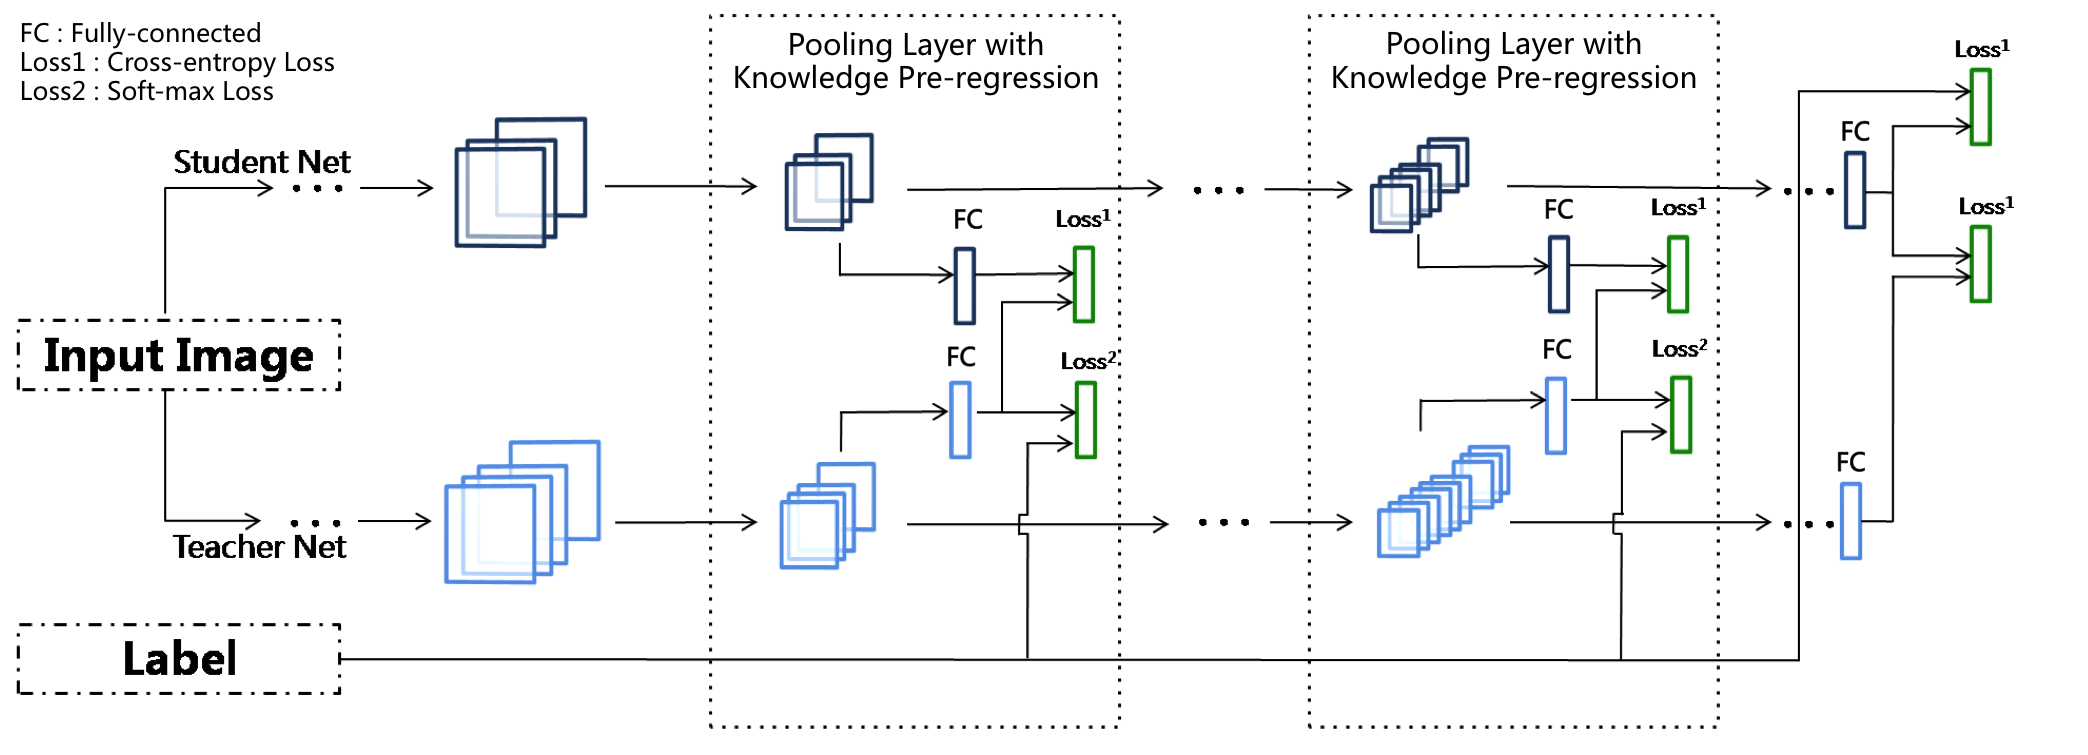
\includegraphics[width=1.0\linewidth]{acc_kp.png}
\caption{FastNet训练过程}
\label{fig:train}
\end{figure*}

FASNet网络具有 5.23M 参数数量和 636.70M 的浮点乘加运算,如表~\ref{tab:fast}所示。FASNet的参数规模和计算量较大,很难对其进行部署应用。因此我们采用1比1的主导卷积核分解对FASNet中的卷积层进行参数压缩,得到一个参数和运算规模较小,推断速度更快的网络结构FastNet。FastNet与FASNet的网络结构、参数和运算规模的对比如表~\ref{tab:fast}所示。压缩后的FastNet仅仅具有 0.37M 的参数数量,是FASNet的 7.07\%。在浮点乘加运算上,FastNet是FASNet的 7.17\%,因此FastNet的推断速度会比FASNet快10倍以上。

\begin{table}[h]
\caption{FASNet与FastNet参数与运算规模对比。}
\label{tab:fast}
\centering
\begin{tabular}{ccc|ccc}
\hline
\multicolumn{3}{c|}{\heiti FASNet} & \multicolumn{3}{c}{\heiti FastNet(1比1)} \\
\cline{1-3}
\cline{4-6}
{\heiti 结构} & {\heiti 参数} & {\heiti 浮点运算} & {\heiti 结构} & {\heiti 参数} & {\heiti 浮点运算} \\
\midrule[1pt]
卷积层 & 1.73 K & 1.77 M & 卷积层  & 1.73 K & 1.77 M\\
卷积层 & 73.73 K & 75.50 M & DK卷积层 & 8.77 K & 8.98 M\\
\hline
SAP池化层  & - & - & SAP池化层  & - & - \\
\hline
SAM卷积层 & 0.38 M & 97.52 M & DK卷积层 & 17.54 K & 4.49 M \\
SAM卷积层 & 0.38 M & 97.52 M & DK卷积层 & 17.54 K & 4.49 M\\
SAM卷积层 & 0.43 M & 110.10 M & DK卷积层 & 33.92 K & 8.68 M\\
\hline
SAP池化层  & - & - & SAP池化层  & - & - \\
\hline
SAM卷积层 & 1.27 M & 81.26 M & DK卷积层 & 67.84 K & 4.34 M \\
SAM卷积层 & 1.27 M & 81.26 M & DK卷积层 & 67.84 K & 4.34 M \\
SAM卷积层 & 1.43 M & 91.75 & DK卷积层 & 0.13 M & 8.54 M\\
\hline
全局池化  & - & - & SAP池化层  & - & - \\
\hline
全连接层 & 22.02 K & 22.02 K & 全连接层 & 22.02 K & 22.02 K \\
\hline
softmax层 & - & - & SAP池化层  & - & - \\
\midrule[1pt]
合计 & 5.23 M & 636.70 M & 合计  & 0.37 M & 45.65 M \\
 \bottomrule[1.5pt]
\end{tabular}
\end{table}

采用第四章中知识预回归的训练方法对FastNet进行训练,以FASNet为学习对象,即教师网络,我们对FastNet进行训练,训练过程如图~\ref{fig:train}所示。我们对FASNet和FastNet的3个池化层分别进行预回归训练,在训练过程中,对于教师网络FASNet,我们采用最大池化代替了原网络中的随机区域池化,让FASNet在逐层监督的过程中可以产生相对稳定不变的监督信息,更为有效地指导学生网络FastNet的学习,加快FastNet网络的收敛速度。通过预回归训练,FastNet的取得了99.27\%的识别率。

\begin{figure}[h]
  \centering%
  \begin{subfigure}{0.45\textwidth}
    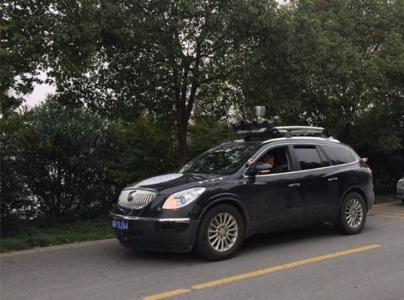
\includegraphics[width=1\linewidth]{tsr_car2.png}
    \caption{THU-IV2。}
  \end{subfigure}%
  \hspace{1em}%
  \begin{subfigure}{0.4\textwidth}
    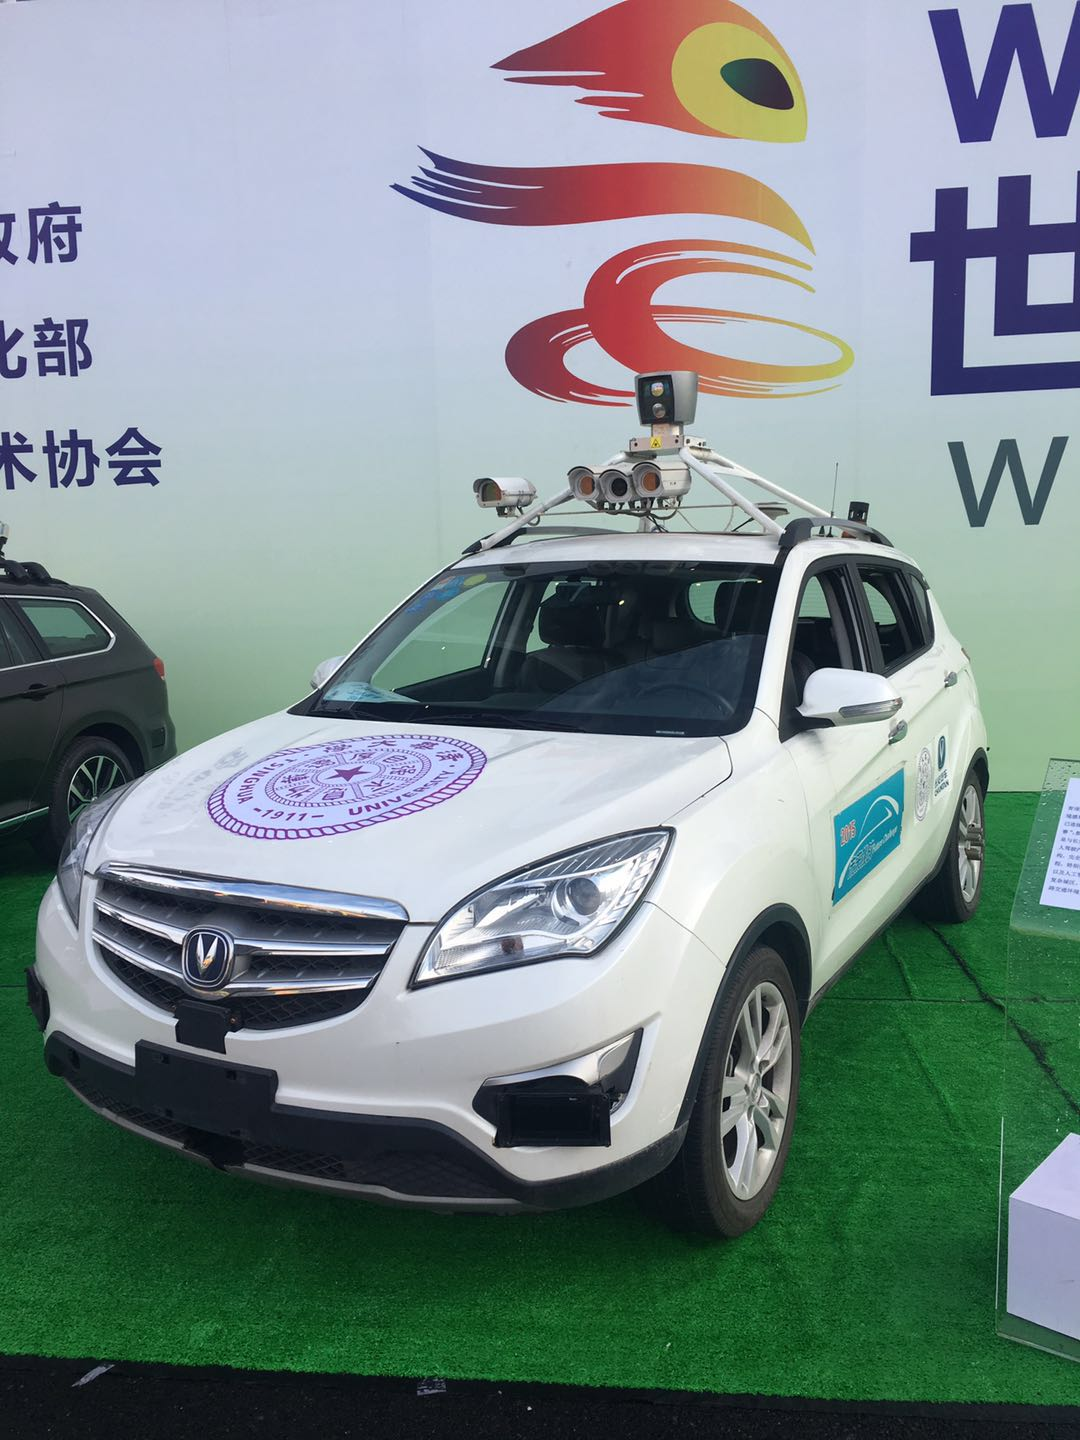
\includegraphics[width=1\linewidth]{tsr_car3.jpg}
    \caption{THU-IV3。}
  \end{subfigure}
  \caption{THU-IV2 和 THU-IV3 第二代与第三代无人驾驶汽车。}
  \label{fig:tsr_car}
\end{figure}

\subsection{无人驾驶汽车上的交通标志检测与识别}

上文中,我们已经成功地实现了基于卷积神经网络的交通标志识别与模型压缩与加速。本小结将讨论在无人驾驶汽车上,交通标志的检测与识别问题。在国家自然科学基金委所支持的重大研究项目”视听觉信息的认知计算“中,我所在的课题组自主研发了 THU-IV1、THU-IV2 和 THU-IV3 三款无人驾驶汽车,其中 THU-IV2 和 THU-IV3 第二代与第三代无人驾驶汽车如图~\ref{fig:tsr_car}所示。基于第三代实验平台 THU-IV3,我们开发了交通标志检测与识别系统。

\begin{figure}[b]
\centering
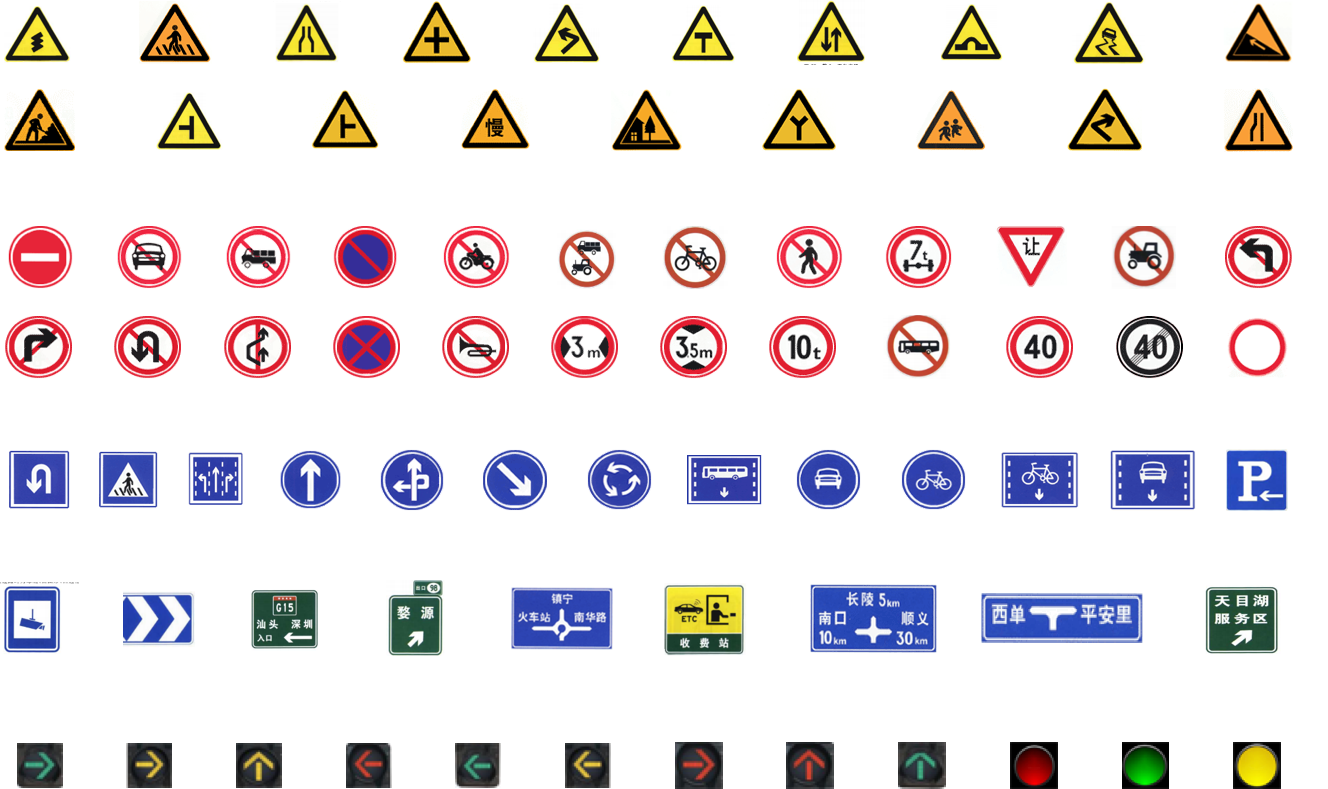
\includegraphics[width=1\linewidth]{tsr_types.png}
\caption{警告标志20类,禁令标志24类,指示标志13类,指路标志9类,交通灯12类。}
\label{fig:tsr_types}
\end{figure}

本章采用场景标注的方式来分割出原始图像中交通标志的位置,来实现交通标志检测的目的。场景标注旨在为输入图像的每一个像素都确定一个语义类别标签,本章采用卷积神经网络对不同位置的图像块进行语义分割,通过语义分割的结果来定位交通标志出现的具体位置。我们采集了2695张具有 $1280\times1024$ 像素大小的离线图像数据集,将其平均分为5份,采用交叉验证的方式,其中四份作为训练集,一份作为测试集。参考 GB5768-2009《道路交通标志和标线》国标中对于交通标志的定位,将交通标志和交通信号灯统一定义为78类,其中包括警告标志20类,禁令标志24类,指示标志13类,指路标志9类,交通灯12类,如图~\ref{fig:tsr_types}。


我们采用如图~\ref{fig:tsr_det2}、图~\ref{fig:tsr_det1}等检测结果类似的图像标注方法,左图对应于原始的输入图像,对于标注图像,我们采用矩形边界框,即形式如(左下角宽度坐标,左下角长度坐标,宽度,长度)的矩形边界框对交通标志进行标注,对于78类不同的交通标志,用1-78这78个整数来填充矩形边界框区域,图像的背景设置为0。尽管矩形边界框的标志方式相对于图像分割任务较为粗略,但是对于本章交通标志识别任务,这样的标志已经完全足够使用。

\begin{figure}
\centering
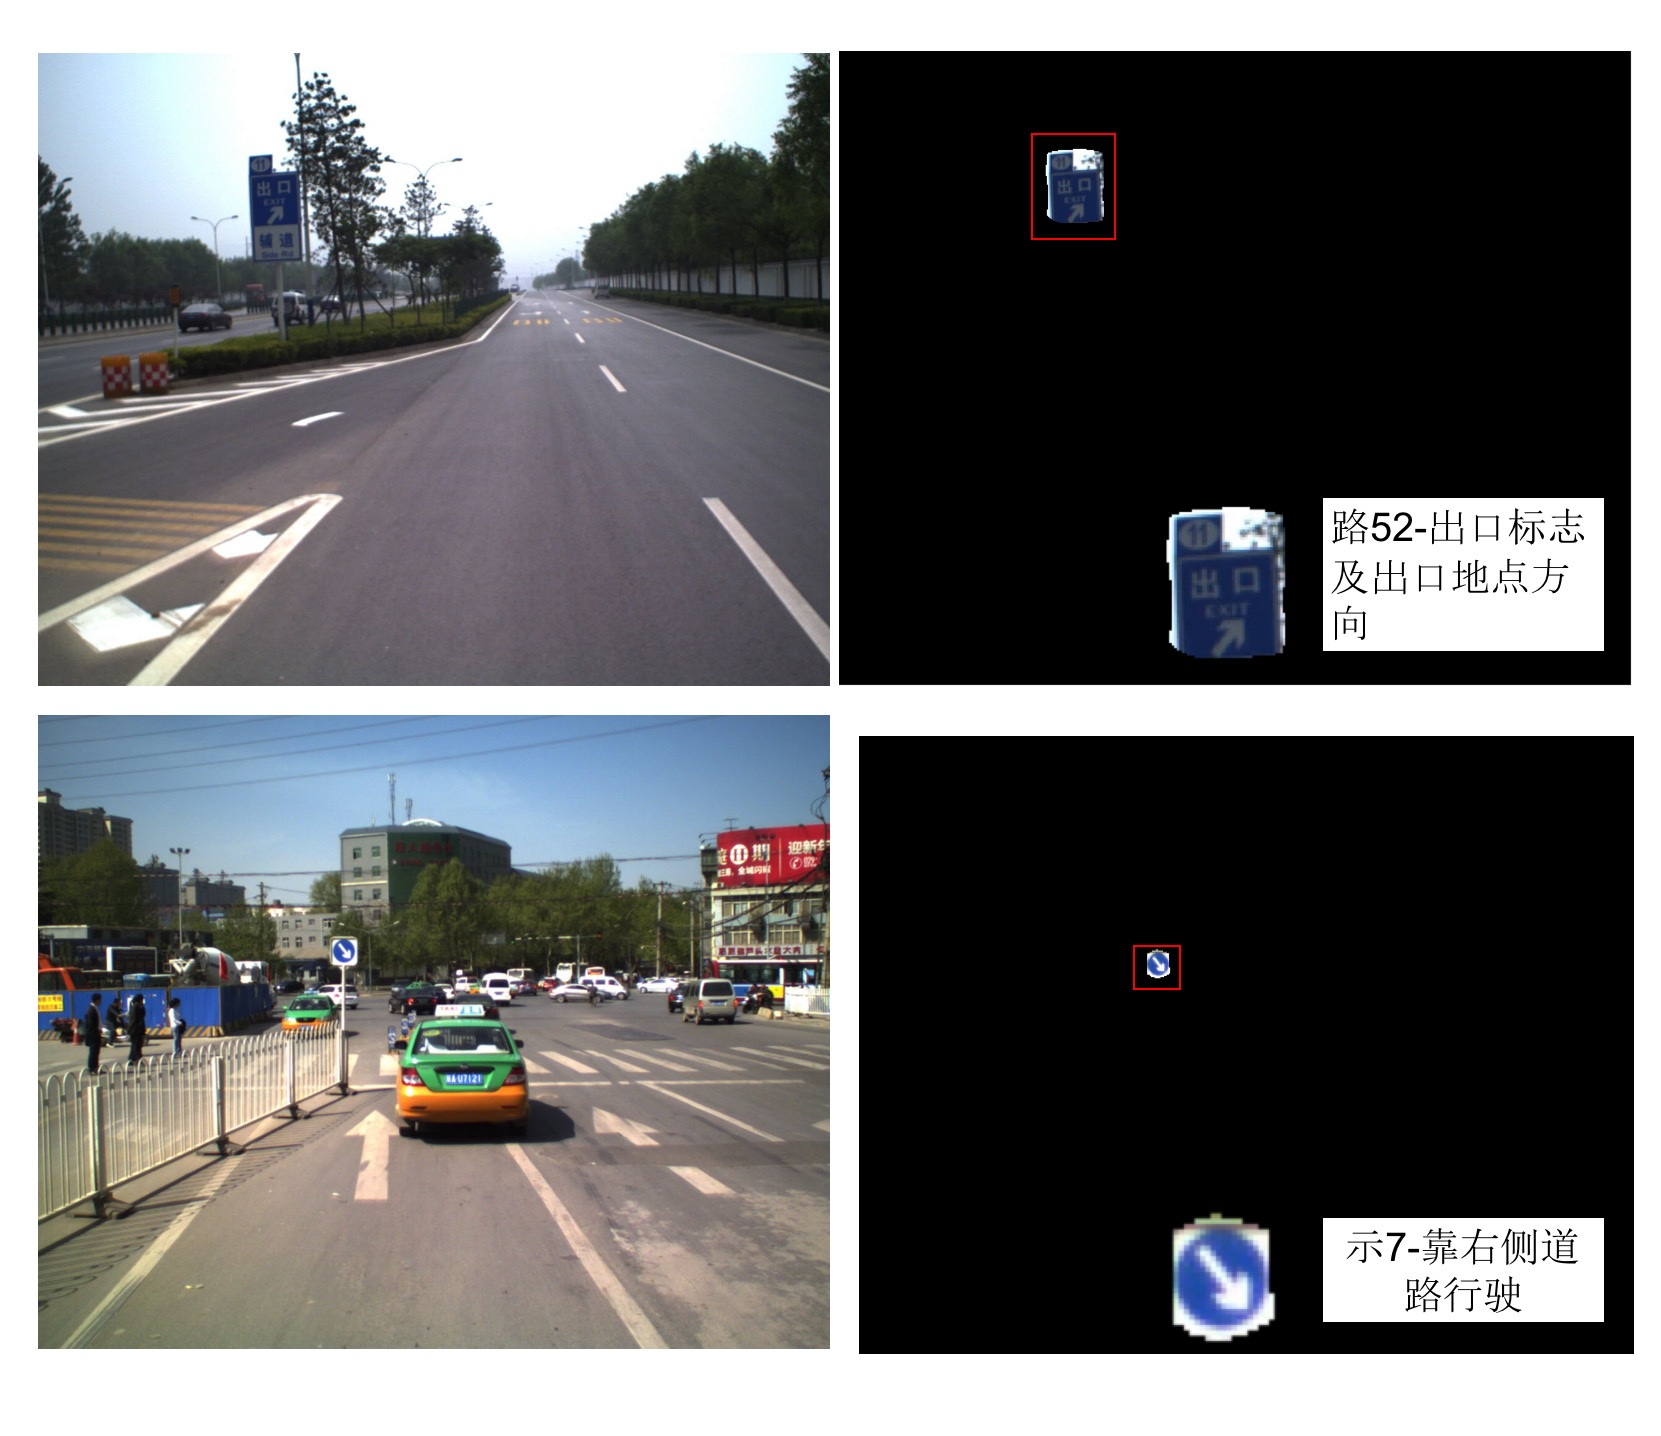
\includegraphics[width=1.0\linewidth]{tsr_det2.jpg}
\caption{指路标志与指示标志分割识别结果。}
\label{fig:tsr_det2}
\end{figure}

\begin{figure}
\centering
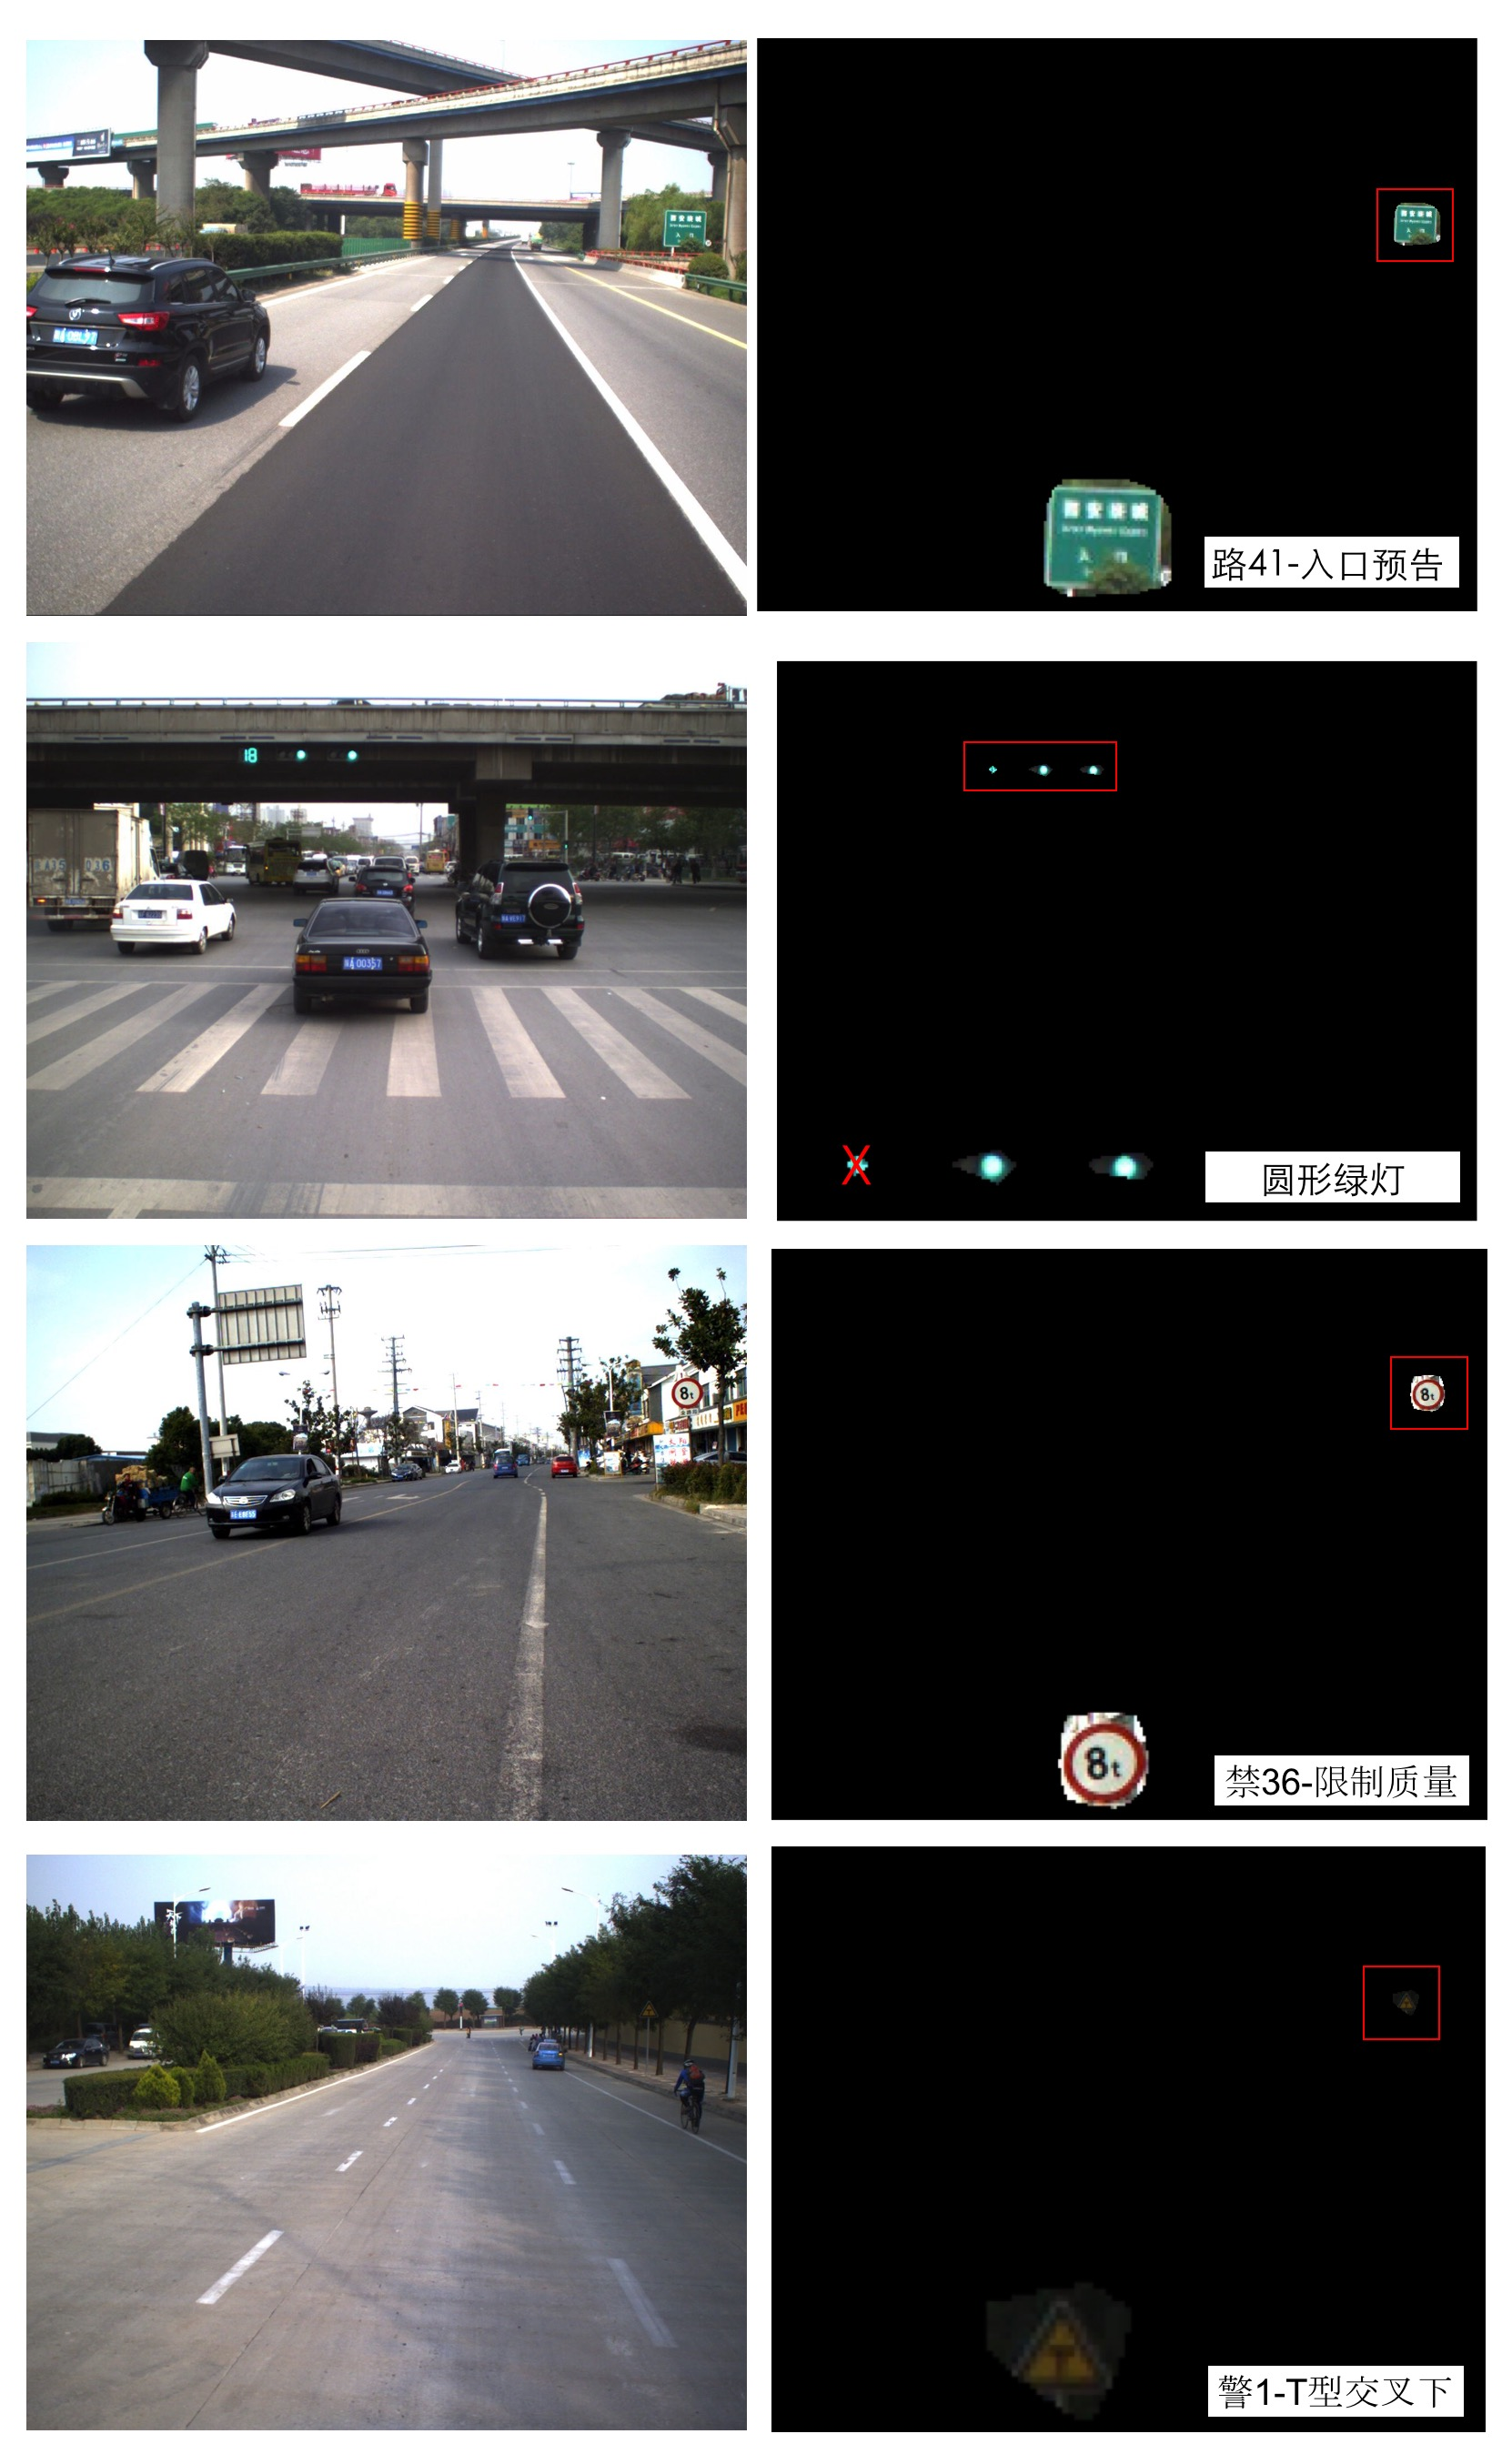
\includegraphics[width=1.0\linewidth]{tsr_det1.jpg}
\caption{指路标志、交通灯、禁令标志、警告标示分割识别结果。}
\label{fig:tsr_det1}
\end{figure}



我们采用上文提出的FASNet卷积神经网络模型进行图像的场景分割,采用全卷积~\cite{long2014fully}的方式进行图像分割,但是与~\cite{long2014fully}不同,我们采用双线性差值的方式对特征图进行上采样,还原成与原始输入图像相同的尺度大小,最后采用Softmax进行逐像素的回归分类。为了提高语义分割网络的性能和训练速度,我们采用第~\ref{app:acc}节在GTSRB数据集上预训练的模型参数对分割网络进行初始化,采用较小的学习率对分割网络进行参数微调。值得注意的是,对于GTSRB交通标志识别任务,仅仅具有43类,需要将其扩展为79类(78个交通标志类别和图像背景)。

在离线测试数据集上,网络的分割结果如图~\ref{fig:tsr_det2}和图~\ref{fig:tsr_det1}所示,图中分别列举了指路标志、交通灯、禁令标志、警告标示和指示标志等交通标志分割结果,对于前景与背景区分度较大的交通标志,分割算法均能取得较好的分割结果。但是对于图~\ref{fig:tsr_det1}中“警1-T型交叉下”交通标志,由于其前景与背景区分度较低,因此分割的边界较为粗略,但分割区域内也包含了完成的交通标志,对于无人驾驶汽车来说已经足够使用。图~\ref{fig:tsr_det1}是圆形交通信号灯的分割,测试结果给出了三个分割结果,但是最左侧的分割结果有误,未能成功的判断出该位置的标示的为红绿灯的剩余时间,而非圆形绿灯。

\section{本章小结}
\label{sec:seg:conclusion}

本章内容是前三章方法的一个综合应用,我们以交通标志识别为应用背景,对组合卷积结构和随机区域池化分别进行了实验验证。组合卷积结构可以有效地提高卷积层的识别能力和网络收敛速度,但是多条特征提取分支加选择器的冗余设计引入了更多的参数和计算量。随机区域池化方法可以在卷积网络的池化层进行特征増广,在基本不引入额外参数与计算量的情况下提高网络的泛化能力。组合卷积结构和随机区域池化作为通用的卷积和池化模块,可以有效地和其他网络结构配合使用。本章我们采用这两种方法构造了FASNet,在德国交通标志识别数据集GTSRB上取得了99.66\%的识别率。针对FASNet网络的参数与计算量较高问题,我们采用第四章中提出的主导卷积核分解方法对网络进行压缩,提出了FastNet结构,并采用知识预回归的训练方法对FastNet进行训练,最终实现了99.27\%的识别率。相对于原始的FASNet网络模型,FastNet具有近10倍的参数压缩比率和预测速度提升。最后,基于 THU-IV3 实验平台,我们进行了交通标志与信号灯的检测与识别实验。











\chapter{总结与展望}
\label{cha:conclusion}

\section{总结}

卷积神经网络在计算机视觉领域,特别是视觉物体识别任务中取得了重大的研究突破,本文从卷积层、池化层和模型压缩与加速三个方面对卷积神经网络进行了改进,并针对交通标志识别问题对这三个方法进行了结合与验证。本文的主要研究内容按章节总结如下:

%第二章提出了一种卷积层的改进方法:自适应卷积模块。卷积层是卷积神经网络最基本的组成结构,具有特征提取的功能。对卷积层的改进主要体现在如何设计一种有效的卷积结构,来增强卷积层的特征提取能力。近年来,很多优秀的网络结构与模型被提出并应用于物体识别任务。
第二章提出了一种卷积层的改进方法:具有组合卷积结构的自适应卷积模块(SAM)。组合卷积结构结合了Inception、Maxout、ResNet和NIN四个优秀网络模型的特点与优势。组合卷积结构以Inception结构为基础计算框架,由四条特征提取分支与一个特征选择器构成。Inception计算框架可以有效地平衡四条分支的参数规模和计算量,四条分支分别对应了不同的特征提取函数,其中包括两条卷积特征提取分支,分别具有不同的网络深度和感受野;一条Maxout分支可以增强组合卷积结构的非线性特征拟合能力;一条ResNet分支可以加快网络的收敛速度;特征选择器可以融合多通道的特征,同时控制特征的维度。Maxout与ResNet分支共享了两条卷积分支的参数,隐层特征的复用可以降低网络的参数规模和计算量,网络参数的复用可以有效避免过拟合现象。在CIFAR-10、CIFAR-100、MNIST和SVHN四个数据集上,我们对SAM进行了测试,分别取得了5.76\%,28.56\%,0.31\%和1.98\%的测试错误率。实验结果表明,使用SAM来搭建卷积神经网络,可以有效地简化网络的设计,同时保持卓越的网络泛化能力。

第三章提出了一种池化层的改进方法:随机区域池化(SAP)。随机区域池化将数据增广的思想扩展到特征层,即特征增广。SAP通过随机仿射变换对池化区域进行重采样,在将传统的池化方法(最大池化或均值池化,本章采用的是最大池化)应用于重采样之后的池化区域。仿射变换后的区域往往处于非整数边界,因此采用双线性差值对非整数边界的像素进行估计。SAP在不改变特征空间样本分布的情况下,扩展特征空间,增加特征的多样性,从而提高网络的泛化能力,使网络对特征的扰动更加鲁棒。在CIFAR-10,CIFAR-100,MNIST和SVHN四个数据集上,我们对SAP进行了测试,分别取得了5.57\%,27.59\%,0.29\%和1.71\%的测试错误率。实验结果表明,SAP在没有明显增加网络参数与计算量的情况上,可以有效地提高网络的泛化能力。

第四章提出了一种网络参数压缩与模型加速的方法:主导卷积核分解(DK分解)和知识预回归(KP训练)。DK分解是受矩阵低秩分解启发而提出的一种卷积参数压缩方法。DK分解将传统的卷积操作分解为特征提取和特征组合两个过程,在特征提取的过程中,对于每个输入特征图,我们仅选择具有主导作用的一个或多个卷积核对其进行特征提取。在特征组合的过程中,我们允许所有中间层特征参与特征的组合。DK分解可以将卷积层的参数和计算量压缩到原来的12\%左右,可以有效地压缩模型的参数,提高网络的预测速度。为了尽量弥补网络因压缩所造成的精度损失,我们提出了知识预回归的训练方法。将原网络(教师网络)部分隐层特征的泛化能力(知识)迁移到压缩后的网络(学生网络),让学生网络尽可能地去学习教师网络的特征表达能力和泛化能力。实验结果表明,知识预回归的训练方法可以加快网络的收敛速度,同时提高网络的泛化能力。

第五章针对无人驾驶或高级辅助驾驶中交通标志识别问题,我们对前三章所提出的方法进行了对比分析。更进一步,我们将三个方法相结合,应用于解决交通标志识别问题。实验结果表明,组合卷积结构和随机区域池化可以有效地与其他卷积网络结构配合使用,提高网络的特征表达能力与网络的泛化能力。本章我们结合两种方法设计了一个具有特征增广的自适应网络模型FASNet,在德国交通标志识别数据集GTSRB上取得了99.66\%的识别率。针对FASNet网络参数和计算量较大的问题,我们采用主导卷积核分解对网络进行了压缩,得到压缩后的快速网络模型FastNet,并采用知识预回归的方法对FastNet进行训练,最终取得了99.27\%的识别率。相对于原始的FASNet网络结构,FastNet具有近10倍的参数压缩和预测速度提升。


\section{展望}

本文从卷积层、池化层、网络参数压缩和训练方法三个方向对卷积神经网络进行了创新,在视觉物体识别任务上取得了一些研究进展,但是在这些研究方向上,仍存在进一步研究与改进的空间。

首先,对于组合卷积结构,目前仅仅在SAM模块中引入了四条特征提取分支。随着卷积神经网络的飞速发展,优秀的网络模型会越来越多,将更多的模型组合到SAM是一个长期积累的过程。将这些优秀结构有效地组合与应用,进一步简化复杂卷积神经网络的设计过程,使卷积神经网络得到更加广泛的应用。此外SAM本身的结构相对较为复杂,导致对于SAM的理解和可视化工作变得非常困难,而网络的可视化工作是理解和优化网络结构的有效手段。

其次,对于特征增广,这是一个提高网络泛化能力的简单有效方法,目前我们仅仅在池化层验证了特征增广的效果。对于卷积神经网络来说,它的一个主要的特点就是分层的特征表达,如何将特征增广应用于更多隐层是一个值得研究的课题。此外对于随机区域池化方法本身,我们仅仅研究了具有旋转、平移和缩放的特征增广方式,我们相信诸如错切、翻转甚至特征空间变换等其他特征增广方式可以进一步提高网络的泛化能力。

最后,对于网络加速,这是卷积神经网络从研究走入实际应用的一个必要环节。在主导卷积核分解的方法中,我们仅仅对卷积层进行了参数压缩,这是因为在我们的应用场景中卷积层占据了几乎全部的参数。而对于其他分类任务,比如百万级别、甚至上亿级别的人脸分类问题,全连接层也会引入大量的参数,如何有效地对全连接层进行DK分解,是一个有有待研究的课题。基于矩阵低秩分解的压缩方法毕竟还是精度有损的压缩,尽管知识预回归弥补了一部分精度损失,但是精度无损的压缩方法仍然是一个有趣的研究课题。




%%% 其它部分
\backmatter

%% 本科生要这几个索引,研究生不要。选择性留下。
% 插图索引
%\listoffigures
% 表格索引
%\listoftables
% 公式索引
%\listofequations


%% 参考文献
% 注意:至少需要引用一篇参考文献,否则下面两行可能引起编译错误。
% 如果不需要参考文献,请将下面两行删除或注释掉。
\bibliographystyle{thuthesis}
\bibliography{ref/myrefs}


%% 致谢
% 如果使用声明扫描页,将可选参数指定为扫描后的 PDF 文件名,例如:
% \begin{acknowledgement}[scan-statement.pdf]
\begin{acknowledgement}
  衷心感谢导师 邓志东 教授对本人的精心指导。邓老师严谨求是的治学精神和勤奋踏实的治学态度将使我终生受益。邓老师为实验室创造了自由宽松的研究氛围,让我能够潜心于自己感兴趣的研究方向。同时感谢邓老师将我带入无人驾驶项目,有机会与业内人士共同学习、探讨、研发无人驾驶技术。
  
  感谢实验室的秘书郭小梅老师,她承担实验室繁杂的运维工作,为实验室的科研生活提供了重要后勤保障和帮助,使我可以专心于科研与项目。
  
  感谢宋亦旭老师对我的鼓励与帮助,宋老师心怀若谷的智者风范、平易近人的人格魅力和一丝不苟的工作作风,让我深感敬佩。
  
  感谢预答辩的各位老师对我论文提出的宝贵建议,让我可以更加顺利地完成博士论文撰写工作。各位老师面对学术,严谨推敲、精益求精的态度,让我在未来的学习工作生活中受益终身。
  
  感谢参与无人车项目的杨博、姚文韬、苏奎峰、周力普、黄振、陈振华、黄竞、陈雄、肖克来提、刘晓龙、杨国润、王诗瑶,他们对无人车做出了巨大的贡献,也在本文的研究过程中给予了我巨大的帮助与启发。与他们一起研发无人车的日日夜夜将使我终生难忘。

  感谢清华大学计算机科学与技术系的老师和同学们对我的帮助和支持。
  
  感谢ThuThesis,让我的博士论文排版增加规范漂亮,让我可以更加专心于论文内容的撰写。
  
\end{acknowledgement}


%% 附录
%\begin{appendix}
%\chapter{外文资料原文}
\label{cha:engorg}

\title{The title of the English paper}

\textbf{Abstract:} As one of the most widely used techniques in operations
research, \emph{ mathematical programming} is defined as a means of maximizing a
quantity known as \emph{bjective function}, subject to a set of constraints
represented by equations and inequalities. Some known subtopics of mathematical
programming are linear programming, nonlinear programming, multiobjective
programming, goal programming, dynamic programming, and multilevel
programming$^{[1]}$.

It is impossible to cover in a single chapter every concept of mathematical
programming. This chapter introduces only the basic concepts and techniques of
mathematical programming such that readers gain an understanding of them
throughout the book$^{[2,3]}$.


\section{Single-Objective Programming}
The general form of single-objective programming (SOP) is written
as follows,
\begin{equation}\tag*{(123)} % 如果附录中的公式不想让它出现在公式索引中,那就请
                             % 用 \tag*{xxxx}
\left\{\begin{array}{l}
\max \,\,f(x)\\[0.1 cm]
\mbox{subject to:} \\ [0.1 cm]
\qquad g_j(x)\le 0,\quad j=1,2,\cdots,p
\end{array}\right.
\end{equation}
which maximizes a real-valued function $f$ of
$x=(x_1,x_2,\cdots,x_n)$ subject to a set of constraints.

\newtheorem{mpdef}{Definition}[chapter]
\begin{mpdef}
In SOP, we call $x$ a decision vector, and
$x_1,x_2,\cdots,x_n$ decision variables. The function
$f$ is called the objective function. The set
\begin{equation}\tag*{(456)} % 这里同理,其它不再一一指定。
S=\left\{x\in\Re^n\bigm|g_j(x)\le 0,\,j=1,2,\cdots,p\right\}
\end{equation}
is called the feasible set. An element $x$ in $S$ is called a
feasible solution.
\end{mpdef}

\newtheorem{mpdefop}[mpdef]{Definition}
\begin{mpdefop}
A feasible solution $x^*$ is called the optimal
solution of SOP if and only if
\begin{equation}
f(x^*)\ge f(x)
\end{equation}
for any feasible solution $x$.
\end{mpdefop}

One of the outstanding contributions to mathematical programming was known as
the Kuhn-Tucker conditions\ref{eq:ktc}. In order to introduce them, let us give
some definitions. An inequality constraint $g_j(x)\le 0$ is said to be active at
a point $x^*$ if $g_j(x^*)=0$. A point $x^*$ satisfying $g_j(x^*)\le 0$ is said
to be regular if the gradient vectors $\nabla g_j(x)$ of all active constraints
are linearly independent.

Let $x^*$ be a regular point of the constraints of SOP and assume that all the
functions $f(x)$ and $g_j(x),j=1,2,\cdots,p$ are differentiable. If $x^*$ is a
local optimal solution, then there exist Lagrange multipliers
$\lambda_j,j=1,2,\cdots,p$ such that the following Kuhn-Tucker conditions hold,
\begin{equation}
\label{eq:ktc}
\left\{\begin{array}{l}
    \nabla f(x^*)-\sum\limits_{j=1}^p\lambda_j\nabla g_j(x^*)=0\\[0.3cm]
    \lambda_jg_j(x^*)=0,\quad j=1,2,\cdots,p\\[0.2cm]
    \lambda_j\ge 0,\quad j=1,2,\cdots,p.
\end{array}\right.
\end{equation}
If all the functions $f(x)$ and $g_j(x),j=1,2,\cdots,p$ are convex and
differentiable, and the point $x^*$ satisfies the Kuhn-Tucker conditions
(\ref{eq:ktc}), then it has been proved that the point $x^*$ is a global optimal
solution of SOP.

\subsection{Linear Programming}
\label{sec:lp}

If the functions $f(x),g_j(x),j=1,2,\cdots,p$ are all linear, then SOP is called
a {\em linear programming}.

The feasible set of linear is always convex. A point $x$ is called an extreme
point of convex set $S$ if $x\in S$ and $x$ cannot be expressed as a convex
combination of two points in $S$. It has been shown that the optimal solution to
linear programming corresponds to an extreme point of its feasible set provided
that the feasible set $S$ is bounded. This fact is the basis of the {\em simplex
  algorithm} which was developed by Dantzig as a very efficient method for
solving linear programming.
\begin{table}[ht]
\centering
  \centering
  \caption*{Table~1\hskip1em This is an example for manually numbered table, which
    would not appear in the list of tables}
  \label{tab:badtabular2}
  \begin{tabular}[c]{|m{1.5cm}|c|c|c|c|c|c|}\hline
    \multicolumn{2}{|c|}{Network Topology} & \# of nodes &
    \multicolumn{3}{c|}{\# of clients} & Server \\\hline
    GT-ITM & Waxman Transit-Stub & 600 &
    \multirow{2}{2em}{2\%}&
    \multirow{2}{2em}{10\%}&
    \multirow{2}{2em}{50\%}&
    \multirow{2}{1.2in}{Max. Connectivity}\\\cline{1-3}
    \multicolumn{2}{|c|}{Inet-2.1} & 6000 & & & &\\\hline
    \multirow{2}{1.5cm}{Xue} & Rui  & Ni &\multicolumn{4}{c|}{\multirow{2}*{\thuthesis}}\\\cline{2-3}
    & \multicolumn{2}{c|}{ABCDEF} &\multicolumn{4}{c|}{} \\\hline
\end{tabular}
\end{table}

Roughly speaking, the simplex algorithm examines only the extreme points of the
feasible set, rather than all feasible points. At first, the simplex algorithm
selects an extreme point as the initial point. The successive extreme point is
selected so as to improve the objective function value. The procedure is
repeated until no improvement in objective function value can be made. The last
extreme point is the optimal solution.

\subsection{Nonlinear Programming}

If at least one of the functions $f(x),g_j(x),j=1,2,\cdots,p$ is nonlinear, then
SOP is called a {\em nonlinear programming}.

A large number of classical optimization methods have been developed to treat
special-structural nonlinear programming based on the mathematical theory
concerned with analyzing the structure of problems.
\begin{figure}[h]
  \centering
  
\includegraphics{thu-lib-logo}
  \caption*{Figure~1\quad This is an example for manually numbered figure,
    which would not appear in the list of figures}
  \label{tab:badfigure2}
\end{figure}

Now we consider a nonlinear programming which is confronted solely with
maximizing a real-valued function with domain $\Re^n$.  Whether derivatives are
available or not, the usual strategy is first to select a point in $\Re^n$ which
is thought to be the most likely place where the maximum exists. If there is no
information available on which to base such a selection, a point is chosen at
random. From this first point an attempt is made to construct a sequence of
points, each of which yields an improved objective function value over its
predecessor. The next point to be added to the sequence is chosen by analyzing
the behavior of the function at the previous points. This construction continues
until some termination criterion is met. Methods based upon this strategy are
called {\em ascent methods}, which can be classified as {\em direct methods},
{\em gradient methods}, and {\em Hessian methods} according to the information
about the behavior of objective function $f$. Direct methods require only that
the function can be evaluated at each point. Gradient methods require the
evaluation of first derivatives of $f$. Hessian methods require the evaluation
of second derivatives. In fact, there is no superior method for all
problems. The efficiency of a method is very much dependent upon the objective
function.

\subsection{Integer Programming}

{\em Integer programming} is a special mathematical programming in which all of
the variables are assumed to be only integer values. When there are not only
integer variables but also conventional continuous variables, we call it {\em
  mixed integer programming}. If all the variables are assumed either 0 or 1,
then the problem is termed a {\em zero-one programming}. Although integer
programming can be solved by an {\em exhaustive enumeration} theoretically, it
is impractical to solve realistically sized integer programming problems. The
most successful algorithm so far found to solve integer programming is called
the {\em branch-and-bound enumeration} developed by Balas (1965) and Dakin
(1965). The other technique to integer programming is the {\em cutting plane
  method} developed by Gomory (1959).

\hfill\textit{Uncertain Programming\/}\quad(\textsl{BaoDing Liu, 2006.2})

\section*{References}
\noindent{\itshape NOTE: These references are only for demonstration. They are
  not real citations in the original text.}

\begin{translationbib}
\item Donald E. Knuth. The \TeX book. Addison-Wesley, 1984. ISBN: 0-201-13448-9
\item Paul W. Abrahams, Karl Berry and Kathryn A. Hargreaves. \TeX\ for the
  Impatient. Addison-Wesley, 1990. ISBN: 0-201-51375-7
\item David Salomon. The advanced \TeX book.  New York : Springer, 1995. ISBN:0-387-94556-3
\end{translationbib}

\chapter{外文资料的调研阅读报告或书面翻译}

\title{英文资料的中文标题}

{\heiti 摘要:} 本章为外文资料翻译内容。如果有摘要可以直接写上来,这部分好像没有
明确的规定。

\section{单目标规划}
北冥有鱼,其名为鲲。鲲之大,不知其几千里也。化而为鸟,其名为鹏。鹏之背,不知其几
千里也。怒而飞,其翼若垂天之云。是鸟也,海运则将徙于南冥。南冥者,天池也。
\begin{equation}\tag*{(123)}
 p(y|\mathbf{x}) = \frac{p(\mathbf{x},y)}{p(\mathbf{x})}=
\frac{p(\mathbf{x}|y)p(y)}{p(\mathbf{x})}
\end{equation}

吾生也有涯,而知也无涯。以有涯随无涯,殆已!已而为知者,殆而已矣!为善无近名,为
恶无近刑,缘督以为经,可以保身,可以全生,可以养亲,可以尽年。

\subsection{线性规划}
庖丁为文惠君解牛,手之所触,肩之所倚,足之所履,膝之所倚,砉然响然,奏刀騞然,莫
不中音,合于桑林之舞,乃中经首之会。
\begin{table}[ht]
\centering
  \centering
  \caption*{表~1\hskip1em 这是手动编号但不出现在索引中的一个表格例子}
  \label{tab:badtabular3}
  \begin{tabular}[c]{|m{1.5cm}|c|c|c|c|c|c|}\hline
    \multicolumn{2}{|c|}{Network Topology} & \# of nodes &
    \multicolumn{3}{c|}{\# of clients} & Server \\\hline
    GT-ITM & Waxman Transit-Stub & 600 &
    \multirow{2}{2em}{2\%}&
    \multirow{2}{2em}{10\%}&
    \multirow{2}{2em}{50\%}&
    \multirow{2}{1.2in}{Max. Connectivity}\\\cline{1-3}
    \multicolumn{2}{|c|}{Inet-2.1} & 6000 & & & &\\\hline
    \multirow{2}{1.5cm}{Xue} & Rui  & Ni &\multicolumn{4}{c|}{\multirow{2}*{\thuthesis}}\\\cline{2-3}
    & \multicolumn{2}{c|}{ABCDEF} &\multicolumn{4}{c|}{} \\\hline
\end{tabular}
\end{table}

文惠君曰:“嘻,善哉!技盖至此乎?”庖丁释刀对曰:“臣之所好者道也,进乎技矣。始臣之
解牛之时,所见无非全牛者;三年之后,未尝见全牛也;方今之时,臣以神遇而不以目视,
官知止而神欲行。依乎天理,批大郤,导大窾,因其固然。技经肯綮之未尝,而况大坬乎!
良庖岁更刀,割也;族庖月更刀,折也;今臣之刀十九年矣,所解数千牛矣,而刀刃若新发
于硎。彼节者有间而刀刃者无厚,以无厚入有间,恢恢乎其于游刃必有余地矣。是以十九年
而刀刃若新发于硎。虽然,每至于族,吾见其难为,怵然为戒,视为止,行为迟,动刀甚微,
謋然已解,如土委地。提刀而立,为之而四顾,为之踌躇满志,善刀而藏之。”

文惠君曰:“善哉!吾闻庖丁之言,得养生焉。”


\subsection{非线性规划}
孔子与柳下季为友,柳下季之弟名曰盗跖。盗跖从卒九千人,横行天下,侵暴诸侯。穴室枢
户,驱人牛马,取人妇女。贪得忘亲,不顾父母兄弟,不祭先祖。所过之邑,大国守城,小
国入保,万民苦之。孔子谓柳下季曰:“夫为人父者,必能诏其子;为人兄者,必能教其弟。
若父不能诏其子,兄不能教其弟,则无贵父子兄弟之亲矣。今先生,世之才士也,弟为盗
跖,为天下害,而弗能教也,丘窃为先生羞之。丘请为先生往说之。”
\begin{figure}[h]
  \centering
  
\includegraphics{thu-whole-logo}
  \caption*{图~1\hskip1em 这是手动编号但不出现索引中的图片的例子}
  \label{tab:badfigure3}
\end{figure}

柳下季曰:“先生言为人父者必能诏其子,为人兄者必能教其弟,若子不听父之诏,弟不受
兄之教,虽今先生之辩,将奈之何哉?且跖之为人也,心如涌泉,意如飘风,强足以距敌,
辩足以饰非。顺其心则喜,逆其心则怒,易辱人以言。先生必无往。”

孔子不听,颜回为驭,子贡为右,往见盗跖。

\subsection{整数规划}
盗跖乃方休卒徒大山之阳,脍人肝而餔之。孔子下车而前,见谒者曰:“鲁人孔丘,闻将军
高义,敬再拜谒者。”谒者入通。盗跖闻之大怒,目如明星,发上指冠,曰:“此夫鲁国之
巧伪人孔丘非邪?为我告之:尔作言造语,妄称文、武,冠枝木之冠,带死牛之胁,多辞缪
说,不耕而食,不织而衣,摇唇鼓舌,擅生是非,以迷天下之主,使天下学士不反其本,妄
作孝弟,而侥幸于封侯富贵者也。子之罪大极重,疾走归!不然,我将以子肝益昼餔之膳。”


\chapter{其它附录}
前面两个附录主要是给本科生做例子。其它附录的内容可以放到这里,当然如果你愿意,可
以把这部分也放到独立的文件中,然后将其 \cs{input} 到主文件中。

%\end{appendix}

%% 个人简历
\begin{resume}

  \resumeitem{个人简历}

  1988 年 8 月 3 日出生于 黑龙江 省  佳木斯 市。

  2007 年 9 月考入 哈尔滨工业大学 大学 计算机科学与技术 系 计算机科学与技术 专业,2011 年 7 月本科毕业并获得 工学学士 学士学位。

  2011 年 9 月进入 清华 大学 计算机 系攻读 博士 学位至今。

  \researchitem{发表的学术论文} % 发表的和录用的合在一起

  % 1. 已经刊载的学术论文(本人是第一作者,或者导师为第一作者本人是第二作者)
  \begin{publications}
    \item  Wang Z Y, Deng Z D, Wang S Y. Accelerating Convolutional Neural Networks with Dominant Convolutional Kernel and Knowledge Pre-regression. European Conference on Computer Vision (ECCV 2016). Springer, 2016: 533-548.
    \item Deng Z D, Wang Z Y, and Wang S Y. Stochastic Area Pooling for Generic Convolutional Neural Network. In Proc. 22nd Conference on Artificial Intelligence (ECAI 2016),  The Hague, Netherlands, 29 August - 02 September 2016, Frontiers in Artificial Intelligence and Applications, vol. 285, pp. 1760 – 1761, 2016. (EI收录,检索号:20170803367829)
     \item Wang Z Y, Deng Z D, Wang S Y. SAM: A Rethinking of Prominent Convolutional Neural Network Architectures for Visual Object Recognition. In Proc. International Joint Conference on Neural Networks (IJCNN 2016), Vancouver, Canada, 24 - 29 July 2016. (EI收录,检索号:	20165203194322)
     \item Wang Z Y, Deng Z D, Huang Z. Traffic Light Detection and Tracking Based on Euclidean Distance Transform and Local Contour Pattern. In Proc. of 2013 Chinese Intelligent Automation Conference. Springer Berlin Heidelberg, 2013: 623-631. (EI 收录,  检索号:20134216853040)
      \item Deng Z D, Wang Z Y, and Wang S Y. Generic Convolutional Neural Network with Random Pooling Area. 6th International Workshop on Combinations of Intelligent Methods and Applications (CIMA 2016). 2016.
  \end{publications}

  % 2. 尚未刊载,但已经接到正式录用函的学术论文(本人为第一作者,或者
  %    导师为第一作者本人是第二作者)。

  % 3. 其他学术论文。可列出除上述两种情况以外的其他学术论文,但必须是
  %    已经刊载或者收到正式录用函的论文。
%  \begin{publications}
%    \item Wu X M, Yang Y, Cai J, et al. Measurements of ferroelectric MEMS
%      microphones. Integrated Ferroelectrics, 2005, 69:417-429. (SCI 收录, 检索号
%      :896KM)
%    \item 贾泽, 杨轶, 陈兢, 等. 用于压电和电容微麦克风的体硅腐蚀相关研究. 压电与声
%      光, 2006, 28(1):117-119. (EI 收录, 检索号:06129773469)
%    \item 伍晓明, 杨轶, 张宁欣, 等. 基于MEMS技术的集成铁电硅微麦克风. 中国集成电路,
%      2003, 53:59-61.
%  \end{publications}

%  \researchitem{研究成果} % 有就写,没有就删除
%  \begin{achievements}
%    \item 任天令, 杨轶, 朱一平, 等. 硅基铁电微声学传感器畴极化区域控制和电极连接的
%      方法: 中国, CN1602118A. (中国专利公开号)
%    \item Ren T L, Yang Y, Zhu Y P, et al. Piezoelectric micro acoustic sensor
%      based on ferroelectric materials: USA, No.11/215, 102. (美国发明专利申请号)
%  \end{achievements}

\end{resume}


%% 本科生进行格式审查是需要下面这个表格,答辩可能不需要。选择性留下。
% 综合论文训练记录表
%\includepdf[pages=-]{scan-record.pdf}
\end{document}
